\documentclass[twoside]{book}

% Packages required by doxygen
\usepackage{fixltx2e}
\usepackage{calc}
\usepackage{doxygen}
\usepackage[export]{adjustbox} % also loads graphicx
\usepackage{graphicx}
\usepackage[utf8]{inputenc}
\usepackage{makeidx}
\usepackage{multicol}
\usepackage{multirow}
\PassOptionsToPackage{warn}{textcomp}
\usepackage{textcomp}
\usepackage[nointegrals]{wasysym}
\usepackage[table]{xcolor}

% Font selection
\usepackage[T1]{fontenc}
\usepackage[scaled=.90]{helvet}
\usepackage{courier}
\usepackage{amssymb}
\usepackage{sectsty}
\renewcommand{\familydefault}{\sfdefault}
\allsectionsfont{%
  \fontseries{bc}\selectfont%
  \color{darkgray}%
}
\renewcommand{\DoxyLabelFont}{%
  \fontseries{bc}\selectfont%
  \color{darkgray}%
}
\newcommand{\+}{\discretionary{\mbox{\scriptsize$\hookleftarrow$}}{}{}}

% Page & text layout
\usepackage{geometry}
\geometry{%
  a4paper,%
  top=2.5cm,%
  bottom=2.5cm,%
  left=2.5cm,%
  right=2.5cm%
}
\tolerance=750
\hfuzz=15pt
\hbadness=750
\setlength{\emergencystretch}{15pt}
\setlength{\parindent}{0cm}
\setlength{\parskip}{3ex plus 2ex minus 2ex}
\makeatletter
\renewcommand{\paragraph}{%
  \@startsection{paragraph}{4}{0ex}{-1.0ex}{1.0ex}{%
    \normalfont\normalsize\bfseries\SS@parafont%
  }%
}
\renewcommand{\subparagraph}{%
  \@startsection{subparagraph}{5}{0ex}{-1.0ex}{1.0ex}{%
    \normalfont\normalsize\bfseries\SS@subparafont%
  }%
}
\makeatother

% Headers & footers
\usepackage{fancyhdr}
\pagestyle{fancyplain}
\fancyhead[LE]{\fancyplain{}{\bfseries\thepage}}
\fancyhead[CE]{\fancyplain{}{}}
\fancyhead[RE]{\fancyplain{}{\bfseries\leftmark}}
\fancyhead[LO]{\fancyplain{}{\bfseries\rightmark}}
\fancyhead[CO]{\fancyplain{}{}}
\fancyhead[RO]{\fancyplain{}{\bfseries\thepage}}
\fancyfoot[LE]{\fancyplain{}{}}
\fancyfoot[CE]{\fancyplain{}{}}
\fancyfoot[RE]{\fancyplain{}{\bfseries\scriptsize Generated by Doxygen }}
\fancyfoot[LO]{\fancyplain{}{\bfseries\scriptsize Generated by Doxygen }}
\fancyfoot[CO]{\fancyplain{}{}}
\fancyfoot[RO]{\fancyplain{}{}}
\renewcommand{\footrulewidth}{0.4pt}
\renewcommand{\chaptermark}[1]{%
  \markboth{#1}{}%
}
\renewcommand{\sectionmark}[1]{%
  \markright{\thesection\ #1}%
}

% Indices & bibliography
\usepackage{natbib}
\usepackage[titles]{tocloft}
\setcounter{tocdepth}{3}
\setcounter{secnumdepth}{5}
\makeindex

% Hyperlinks (required, but should be loaded last)
\usepackage{ifpdf}
\ifpdf
  \usepackage[pdftex,pagebackref=true]{hyperref}
\else
  \usepackage[ps2pdf,pagebackref=true]{hyperref}
\fi
\hypersetup{%
  colorlinks=true,%
  linkcolor=blue,%
  citecolor=blue,%
  unicode%
}

% Custom commands
\newcommand{\clearemptydoublepage}{%
  \newpage{\pagestyle{empty}\cleardoublepage}%
}

\usepackage{caption}
\captionsetup{labelsep=space,justification=centering,font={bf},singlelinecheck=off,skip=4pt,position=top}

%===== C O N T E N T S =====

\begin{document}

% Titlepage & ToC
\hypersetup{pageanchor=false,
             bookmarksnumbered=true,
             pdfencoding=unicode
            }
\pagenumbering{alph}
\begin{titlepage}
\vspace*{7cm}
\begin{center}%
{\Large Sketchy Super Mario Bros. \\[1ex]\large 1 }\\
\vspace*{1cm}
{\large Generated by Doxygen 1.8.13}\\
\end{center}
\end{titlepage}
\clearemptydoublepage
\pagenumbering{roman}
\tableofcontents
\clearemptydoublepage
\pagenumbering{arabic}
\hypersetup{pageanchor=true}

%--- Begin generated contents ---
\chapter{Hierarchical Index}
\section{Class Hierarchy}
This inheritance list is sorted roughly, but not completely, alphabetically\+:\begin{DoxyCompactList}
\item \contentsline{section}{nl.\+arjanfrans.\+mario.\+audio.\+Audio}{\pageref{classnl_1_1arjanfrans_1_1mario_1_1audio_1_1Audio}}{}
\item \contentsline{section}{nl.\+arjanfrans.\+mario.\+graphics.\+Character\+Animation}{\pageref{classnl_1_1arjanfrans_1_1mario_1_1graphics_1_1CharacterAnimation}}{}
\begin{DoxyCompactList}
\item \contentsline{section}{nl.\+arjanfrans.\+mario.\+graphics.\+Goomba\+Animation}{\pageref{classnl_1_1arjanfrans_1_1mario_1_1graphics_1_1GoombaAnimation}}{}
\item \contentsline{section}{nl.\+arjanfrans.\+mario.\+graphics.\+Mario\+Animation}{\pageref{classnl_1_1arjanfrans_1_1mario_1_1graphics_1_1MarioAnimation}}{}
\end{DoxyCompactList}
\item \contentsline{section}{nl.\+arjanfrans.\+mario.\+debug.\+D}{\pageref{classnl_1_1arjanfrans_1_1mario_1_1debug_1_1D}}{}
\item \contentsline{section}{nl.\+arjanfrans.\+mario.\+desktop.\+Desktop\+Launcher}{\pageref{classnl_1_1arjanfrans_1_1mario_1_1desktop_1_1DesktopLauncher}}{}
\item \contentsline{section}{nl.\+arjanfrans.\+mario.\+view.\+Parallax\+Background}{\pageref{classnl_1_1arjanfrans_1_1mario_1_1view_1_1ParallaxBackground}}{}
\item \contentsline{section}{nl.\+arjanfrans.\+mario.\+view.\+Parallax\+Layer}{\pageref{classnl_1_1arjanfrans_1_1mario_1_1view_1_1ParallaxLayer}}{}
\item \contentsline{section}{nl.\+arjanfrans.\+mario.\+graphics.\+Tiles}{\pageref{classnl_1_1arjanfrans_1_1mario_1_1graphics_1_1Tiles}}{}
\item \contentsline{section}{nl.\+arjanfrans.\+mario.\+model.\+World}{\pageref{classnl_1_1arjanfrans_1_1mario_1_1model_1_1World}}{}
\item \contentsline{section}{nl.\+arjanfrans.\+mario.\+view.\+World\+Renderer}{\pageref{classnl_1_1arjanfrans_1_1mario_1_1view_1_1WorldRenderer}}{}
\item Actions\begin{DoxyCompactList}
\item \contentsline{section}{nl.\+arjanfrans.\+mario.\+actions.\+Actor\+Actions}{\pageref{classnl_1_1arjanfrans_1_1mario_1_1actions_1_1ActorActions}}{}
\item \contentsline{section}{nl.\+arjanfrans.\+mario.\+actions.\+Mario\+Actions}{\pageref{classnl_1_1arjanfrans_1_1mario_1_1actions_1_1MarioActions}}{}
\item \contentsline{section}{nl.\+arjanfrans.\+mario.\+actions.\+Moveable\+Actions}{\pageref{classnl_1_1arjanfrans_1_1mario_1_1actions_1_1MoveableActions}}{}
\end{DoxyCompactList}
\item Actor\begin{DoxyCompactList}
\item \contentsline{section}{nl.\+arjanfrans.\+mario.\+model.\+Flag}{\pageref{classnl_1_1arjanfrans_1_1mario_1_1model_1_1Flag}}{}
\item \contentsline{section}{nl.\+arjanfrans.\+mario.\+model.\+Item}{\pageref{classnl_1_1arjanfrans_1_1mario_1_1model_1_1Item}}{}
\item \contentsline{section}{nl.\+arjanfrans.\+mario.\+model.\+Moving\+Actor}{\pageref{classnl_1_1arjanfrans_1_1mario_1_1model_1_1MovingActor}}{}
\begin{DoxyCompactList}
\item \contentsline{section}{nl.\+arjanfrans.\+mario.\+model.\+Creature}{\pageref{classnl_1_1arjanfrans_1_1mario_1_1model_1_1Creature}}{}
\begin{DoxyCompactList}
\item \contentsline{section}{nl.\+arjanfrans.\+mario.\+model.\+Goomba}{\pageref{classnl_1_1arjanfrans_1_1mario_1_1model_1_1Goomba}}{}
\item \contentsline{section}{nl.\+arjanfrans.\+mario.\+model.\+Mario}{\pageref{classnl_1_1arjanfrans_1_1mario_1_1model_1_1Mario}}{}
\end{DoxyCompactList}
\item \contentsline{section}{nl.\+arjanfrans.\+mario.\+model.\+Mushroom}{\pageref{classnl_1_1arjanfrans_1_1mario_1_1model_1_1Mushroom}}{}
\begin{DoxyCompactList}
\item \contentsline{section}{nl.\+arjanfrans.\+mario.\+model.\+Super}{\pageref{classnl_1_1arjanfrans_1_1mario_1_1model_1_1Super}}{}
\end{DoxyCompactList}
\end{DoxyCompactList}
\item \contentsline{section}{nl.\+arjanfrans.\+mario.\+model.\+Static\+Actor}{\pageref{classnl_1_1arjanfrans_1_1mario_1_1model_1_1StaticActor}}{}
\begin{DoxyCompactList}
\item \contentsline{section}{nl.\+arjanfrans.\+mario.\+model.\+Brick}{\pageref{classnl_1_1arjanfrans_1_1mario_1_1model_1_1Brick}}{}
\end{DoxyCompactList}
\end{DoxyCompactList}
\item Game\begin{DoxyCompactList}
\item \contentsline{section}{nl.\+arjanfrans.\+mario.\+Mario\+Game}{\pageref{classnl_1_1arjanfrans_1_1mario_1_1MarioGame}}{}
\end{DoxyCompactList}
\item Input\+Listener\begin{DoxyCompactList}
\item \contentsline{section}{nl.\+arjanfrans.\+mario.\+input.\+Mario\+Input}{\pageref{classnl_1_1arjanfrans_1_1mario_1_1input_1_1MarioInput}}{}
\end{DoxyCompactList}
\item Sprite\begin{DoxyCompactList}
\item \contentsline{section}{nl.\+arjanfrans.\+mario.\+model.\+brick.\+Brick\+Piece}{\pageref{classnl_1_1arjanfrans_1_1mario_1_1model_1_1brick_1_1BrickPiece}}{}
\item \contentsline{section}{nl.\+arjanfrans.\+mario.\+model.\+brick.\+Brick\+Shatter}{\pageref{classnl_1_1arjanfrans_1_1mario_1_1model_1_1brick_1_1BrickShatter}}{}
\end{DoxyCompactList}
\item Tiled\+Map\+Tile\begin{DoxyCompactList}
\item \contentsline{section}{nl.\+arjanfrans.\+mario.\+model.\+Tile}{\pageref{classnl_1_1arjanfrans_1_1mario_1_1model_1_1Tile}}{}
\end{DoxyCompactList}
\end{DoxyCompactList}

\chapter{Class Index}
\section{Class List}
Here are the classes, structs, unions and interfaces with brief descriptions\+:\begin{DoxyCompactList}
\item\contentsline{section}{\hyperlink{classnl_1_1arjanfrans_1_1mario_1_1actions_1_1ActorActions}{nl.\+arjanfrans.\+mario.\+actions.\+Actor\+Actions} \\*Inherited class Actions }{\pageref{classnl_1_1arjanfrans_1_1mario_1_1actions_1_1ActorActions}}{}
\item\contentsline{section}{\hyperlink{classnl_1_1arjanfrans_1_1mario_1_1audio_1_1Audio}{nl.\+arjanfrans.\+mario.\+audio.\+Audio} \\*This is a class that implements the audio in the game }{\pageref{classnl_1_1arjanfrans_1_1mario_1_1audio_1_1Audio}}{}
\item\contentsline{section}{\hyperlink{classnl_1_1arjanfrans_1_1mario_1_1model_1_1Brick}{nl.\+arjanfrans.\+mario.\+model.\+Brick} \\*This class is the class meant to model the bricks in the game }{\pageref{classnl_1_1arjanfrans_1_1mario_1_1model_1_1Brick}}{}
\item\contentsline{section}{\hyperlink{classnl_1_1arjanfrans_1_1mario_1_1model_1_1brick_1_1BrickPiece}{nl.\+arjanfrans.\+mario.\+model.\+brick.\+Brick\+Piece} \\*This class is the class meant to model the pieces of the bricks in the game }{\pageref{classnl_1_1arjanfrans_1_1mario_1_1model_1_1brick_1_1BrickPiece}}{}
\item\contentsline{section}{\hyperlink{classnl_1_1arjanfrans_1_1mario_1_1model_1_1brick_1_1BrickShatter}{nl.\+arjanfrans.\+mario.\+model.\+brick.\+Brick\+Shatter} \\*This class is the class meant to model the shattering of the bricks in the game }{\pageref{classnl_1_1arjanfrans_1_1mario_1_1model_1_1brick_1_1BrickShatter}}{}
\item\contentsline{section}{\hyperlink{classnl_1_1arjanfrans_1_1mario_1_1graphics_1_1CharacterAnimation}{nl.\+arjanfrans.\+mario.\+graphics.\+Character\+Animation} \\*This is an abstract class that will be implemented to handle the animations of various characters in the game }{\pageref{classnl_1_1arjanfrans_1_1mario_1_1graphics_1_1CharacterAnimation}}{}
\item\contentsline{section}{\hyperlink{classnl_1_1arjanfrans_1_1mario_1_1model_1_1Creature}{nl.\+arjanfrans.\+mario.\+model.\+Creature} \\*This class is the class model to represent any moving actor that is interactive, and not \hyperlink{classnl_1_1arjanfrans_1_1mario_1_1model_1_1Mario}{Mario} }{\pageref{classnl_1_1arjanfrans_1_1mario_1_1model_1_1Creature}}{}
\item\contentsline{section}{\hyperlink{classnl_1_1arjanfrans_1_1mario_1_1debug_1_1D}{nl.\+arjanfrans.\+mario.\+debug.\+D} \\*Debug class }{\pageref{classnl_1_1arjanfrans_1_1mario_1_1debug_1_1D}}{}
\item\contentsline{section}{\hyperlink{classnl_1_1arjanfrans_1_1mario_1_1desktop_1_1DesktopLauncher}{nl.\+arjanfrans.\+mario.\+desktop.\+Desktop\+Launcher} \\*This class is the main method allowing the game to initialize and launch }{\pageref{classnl_1_1arjanfrans_1_1mario_1_1desktop_1_1DesktopLauncher}}{}
\item\contentsline{section}{\hyperlink{classnl_1_1arjanfrans_1_1mario_1_1model_1_1Flag}{nl.\+arjanfrans.\+mario.\+model.\+Flag} \\*This flag represents the flag pole at the end of the stage that completes if \hyperlink{classnl_1_1arjanfrans_1_1mario_1_1model_1_1Mario}{Mario} interacts with it }{\pageref{classnl_1_1arjanfrans_1_1mario_1_1model_1_1Flag}}{}
\item\contentsline{section}{\hyperlink{classnl_1_1arjanfrans_1_1mario_1_1model_1_1Goomba}{nl.\+arjanfrans.\+mario.\+model.\+Goomba} \\*\hyperlink{classnl_1_1arjanfrans_1_1mario_1_1model_1_1Goomba}{Goomba} represents the \hyperlink{classnl_1_1arjanfrans_1_1mario_1_1model_1_1Goomba}{Goomba} enemies from the original \hyperlink{classnl_1_1arjanfrans_1_1mario_1_1model_1_1Mario}{Mario} game }{\pageref{classnl_1_1arjanfrans_1_1mario_1_1model_1_1Goomba}}{}
\item\contentsline{section}{\hyperlink{classnl_1_1arjanfrans_1_1mario_1_1graphics_1_1GoombaAnimation}{nl.\+arjanfrans.\+mario.\+graphics.\+Goomba\+Animation} \\*This is a class that implements the abstract class, \hyperlink{classnl_1_1arjanfrans_1_1mario_1_1graphics_1_1CharacterAnimation}{Character\+Animation}, specifically for the animation of the Goomba character }{\pageref{classnl_1_1arjanfrans_1_1mario_1_1graphics_1_1GoombaAnimation}}{}
\item\contentsline{section}{\hyperlink{classnl_1_1arjanfrans_1_1mario_1_1model_1_1Item}{nl.\+arjanfrans.\+mario.\+model.\+Item} \\*Represents any item in game }{\pageref{classnl_1_1arjanfrans_1_1mario_1_1model_1_1Item}}{}
\item\contentsline{section}{\hyperlink{classnl_1_1arjanfrans_1_1mario_1_1model_1_1Mario}{nl.\+arjanfrans.\+mario.\+model.\+Mario} \\*Represents the playable character in the game }{\pageref{classnl_1_1arjanfrans_1_1mario_1_1model_1_1Mario}}{}
\item\contentsline{section}{\hyperlink{classnl_1_1arjanfrans_1_1mario_1_1actions_1_1MarioActions}{nl.\+arjanfrans.\+mario.\+actions.\+Mario\+Actions} \\*Inherited class Actions }{\pageref{classnl_1_1arjanfrans_1_1mario_1_1actions_1_1MarioActions}}{}
\item\contentsline{section}{\hyperlink{classnl_1_1arjanfrans_1_1mario_1_1graphics_1_1MarioAnimation}{nl.\+arjanfrans.\+mario.\+graphics.\+Mario\+Animation} \\*This is a class that implements the abstract class, \hyperlink{classnl_1_1arjanfrans_1_1mario_1_1graphics_1_1CharacterAnimation}{Character\+Animation}, specifically for the animation of Mario }{\pageref{classnl_1_1arjanfrans_1_1mario_1_1graphics_1_1MarioAnimation}}{}
\item\contentsline{section}{\hyperlink{classnl_1_1arjanfrans_1_1mario_1_1MarioGame}{nl.\+arjanfrans.\+mario.\+Mario\+Game} \\*The class meant to render the game }{\pageref{classnl_1_1arjanfrans_1_1mario_1_1MarioGame}}{}
\item\contentsline{section}{\hyperlink{classnl_1_1arjanfrans_1_1mario_1_1input_1_1MarioInput}{nl.\+arjanfrans.\+mario.\+input.\+Mario\+Input} \\*Inherited class that overrides mario input methods }{\pageref{classnl_1_1arjanfrans_1_1mario_1_1input_1_1MarioInput}}{}
\item\contentsline{section}{\hyperlink{classnl_1_1arjanfrans_1_1mario_1_1actions_1_1MoveableActions}{nl.\+arjanfrans.\+mario.\+actions.\+Moveable\+Actions} \\*Inherited class Actions }{\pageref{classnl_1_1arjanfrans_1_1mario_1_1actions_1_1MoveableActions}}{}
\item\contentsline{section}{\hyperlink{classnl_1_1arjanfrans_1_1mario_1_1model_1_1MovingActor}{nl.\+arjanfrans.\+mario.\+model.\+Moving\+Actor} \\*Represents a moving actor in the game }{\pageref{classnl_1_1arjanfrans_1_1mario_1_1model_1_1MovingActor}}{}
\item\contentsline{section}{\hyperlink{classnl_1_1arjanfrans_1_1mario_1_1model_1_1Mushroom}{nl.\+arjanfrans.\+mario.\+model.\+Mushroom} \\*Inherited class \hyperlink{classnl_1_1arjanfrans_1_1mario_1_1model_1_1MovingActor}{Moving\+Actor} }{\pageref{classnl_1_1arjanfrans_1_1mario_1_1model_1_1Mushroom}}{}
\item\contentsline{section}{\hyperlink{classnl_1_1arjanfrans_1_1mario_1_1view_1_1ParallaxBackground}{nl.\+arjanfrans.\+mario.\+view.\+Parallax\+Background} \\*The class meant to create a parallax background }{\pageref{classnl_1_1arjanfrans_1_1mario_1_1view_1_1ParallaxBackground}}{}
\item\contentsline{section}{\hyperlink{classnl_1_1arjanfrans_1_1mario_1_1view_1_1ParallaxLayer}{nl.\+arjanfrans.\+mario.\+view.\+Parallax\+Layer} \\*The class meant to retrieve a layer from a \hyperlink{classnl_1_1arjanfrans_1_1mario_1_1view_1_1ParallaxBackground}{Parallax\+Background} }{\pageref{classnl_1_1arjanfrans_1_1mario_1_1view_1_1ParallaxLayer}}{}
\item\contentsline{section}{\hyperlink{classnl_1_1arjanfrans_1_1mario_1_1model_1_1StaticActor}{nl.\+arjanfrans.\+mario.\+model.\+Static\+Actor} \\*Inherited class that represents static actor }{\pageref{classnl_1_1arjanfrans_1_1mario_1_1model_1_1StaticActor}}{}
\item\contentsline{section}{\hyperlink{classnl_1_1arjanfrans_1_1mario_1_1model_1_1Super}{nl.\+arjanfrans.\+mario.\+model.\+Super} \\*Inherited class that overrides \hyperlink{classnl_1_1arjanfrans_1_1mario_1_1model_1_1Mushroom}{Mushroom} methods that represents mario in super state }{\pageref{classnl_1_1arjanfrans_1_1mario_1_1model_1_1Super}}{}
\item\contentsline{section}{\hyperlink{classnl_1_1arjanfrans_1_1mario_1_1model_1_1Tile}{nl.\+arjanfrans.\+mario.\+model.\+Tile} }{\pageref{classnl_1_1arjanfrans_1_1mario_1_1model_1_1Tile}}{}
\item\contentsline{section}{\hyperlink{classnl_1_1arjanfrans_1_1mario_1_1graphics_1_1Tiles}{nl.\+arjanfrans.\+mario.\+graphics.\+Tiles} \\*This is a class meant to deal with the tiles that make up the graphics of the game }{\pageref{classnl_1_1arjanfrans_1_1mario_1_1graphics_1_1Tiles}}{}
\item\contentsline{section}{\hyperlink{classnl_1_1arjanfrans_1_1mario_1_1model_1_1World}{nl.\+arjanfrans.\+mario.\+model.\+World} \\*Represents world }{\pageref{classnl_1_1arjanfrans_1_1mario_1_1model_1_1World}}{}
\item\contentsline{section}{\hyperlink{classnl_1_1arjanfrans_1_1mario_1_1view_1_1WorldRenderer}{nl.\+arjanfrans.\+mario.\+view.\+World\+Renderer} \\*Render of world }{\pageref{classnl_1_1arjanfrans_1_1mario_1_1view_1_1WorldRenderer}}{}
\end{DoxyCompactList}

\chapter{File Index}
\section{File List}
Here is a list of all documented files with brief descriptions\+:\begin{DoxyCompactList}
\item\contentsline{section}{core/src/nl/arjanfrans/mario/actions/\hyperlink{ActorActions_8java}{Actor\+Actions.\+java} }{\pageref{ActorActions_8java}}{}
\item\contentsline{section}{core/src/nl/arjanfrans/mario/actions/\hyperlink{MarioActions_8java}{Mario\+Actions.\+java} }{\pageref{MarioActions_8java}}{}
\item\contentsline{section}{core/src/nl/arjanfrans/mario/actions/\hyperlink{MoveableActions_8java}{Moveable\+Actions.\+java} }{\pageref{MoveableActions_8java}}{}
\item\contentsline{section}{core/src/nl/arjanfrans/mario/debug/\hyperlink{D_8java}{D.\+java} }{\pageref{D_8java}}{}
\item\contentsline{section}{core/src/nl/arjanfrans/mario/input/\hyperlink{MarioInput_8java}{Mario\+Input.\+java} }{\pageref{MarioInput_8java}}{}
\item\contentsline{section}{core/src/nl/arjanfrans/mario/model/\hyperlink{Creature_8java}{Creature.\+java} }{\pageref{Creature_8java}}{}
\item\contentsline{section}{core/src/nl/arjanfrans/mario/model/\hyperlink{Flag_8java}{Flag.\+java} }{\pageref{Flag_8java}}{}
\item\contentsline{section}{core/src/nl/arjanfrans/mario/model/\hyperlink{Goomba_8java}{Goomba.\+java} }{\pageref{Goomba_8java}}{}
\item\contentsline{section}{core/src/nl/arjanfrans/mario/model/\hyperlink{Item_8java}{Item.\+java} }{\pageref{Item_8java}}{}
\item\contentsline{section}{core/src/nl/arjanfrans/mario/model/\hyperlink{Mario_8java}{Mario.\+java} }{\pageref{Mario_8java}}{}
\item\contentsline{section}{core/src/nl/arjanfrans/mario/model/\hyperlink{Mushroom_8java}{Mushroom.\+java} }{\pageref{Mushroom_8java}}{}
\item\contentsline{section}{core/src/nl/arjanfrans/mario/model/\hyperlink{StaticActor_8java}{Static\+Actor.\+java} }{\pageref{StaticActor_8java}}{}
\item\contentsline{section}{core/src/nl/arjanfrans/mario/model/\hyperlink{Super_8java}{Super.\+java} }{\pageref{Super_8java}}{}
\item\contentsline{section}{core/src/nl/arjanfrans/mario/model/\hyperlink{World_8java}{World.\+java} }{\pageref{World_8java}}{}
\item\contentsline{section}{core/src/nl/arjanfrans/mario/view/\hyperlink{WorldRenderer_8java}{World\+Renderer.\+java} }{\pageref{WorldRenderer_8java}}{}
\item\contentsline{section}{desktop/src/nl/arjanfrans/mario/desktop/\hyperlink{DesktopLauncher_8java}{Desktop\+Launcher.\+java} }{\pageref{DesktopLauncher_8java}}{}
\end{DoxyCompactList}

\chapter{Class Documentation}
\hypertarget{classnl_1_1arjanfrans_1_1mario_1_1actions_1_1ActorActions}{}\section{nl.\+arjanfrans.\+mario.\+actions.\+Actor\+Actions Class Reference}
\label{classnl_1_1arjanfrans_1_1mario_1_1actions_1_1ActorActions}\index{nl.\+arjanfrans.\+mario.\+actions.\+Actor\+Actions@{nl.\+arjanfrans.\+mario.\+actions.\+Actor\+Actions}}


Inherited class Actions.  




Inheritance diagram for nl.\+arjanfrans.\+mario.\+actions.\+Actor\+Actions\+:\nopagebreak
\begin{figure}[H]
\begin{center}
\leavevmode
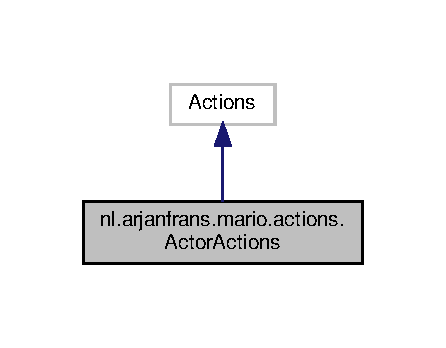
\includegraphics[width=214pt]{classnl_1_1arjanfrans_1_1mario_1_1actions_1_1ActorActions__inherit__graph}
\end{center}
\end{figure}


Collaboration diagram for nl.\+arjanfrans.\+mario.\+actions.\+Actor\+Actions\+:\nopagebreak
\begin{figure}[H]
\begin{center}
\leavevmode
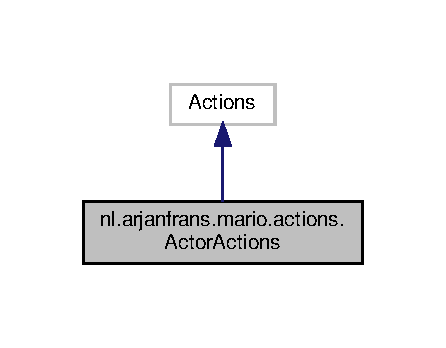
\includegraphics[width=214pt]{classnl_1_1arjanfrans_1_1mario_1_1actions_1_1ActorActions__coll__graph}
\end{center}
\end{figure}
\subsection*{Classes}
\begin{DoxyCompactItemize}
\item 
class {\bfseries remove\+Actor}
\begin{DoxyCompactList}\small\item\em Inherited class Action. \end{DoxyCompactList}\end{DoxyCompactItemize}


\subsection{Detailed Description}
Inherited class Actions. 

The documentation for this class was generated from the following file\+:\begin{DoxyCompactItemize}
\item 
core/src/nl/arjanfrans/mario/actions/\hyperlink{ActorActions_8java}{Actor\+Actions.\+java}\end{DoxyCompactItemize}

\hypertarget{classnl_1_1arjanfrans_1_1mario_1_1audio_1_1Audio}{}\section{nl.\+arjanfrans.\+mario.\+audio.\+Audio Class Reference}
\label{classnl_1_1arjanfrans_1_1mario_1_1audio_1_1Audio}\index{nl.\+arjanfrans.\+mario.\+audio.\+Audio@{nl.\+arjanfrans.\+mario.\+audio.\+Audio}}


This is a class that implements the audio in the game.  




Collaboration diagram for nl.\+arjanfrans.\+mario.\+audio.\+Audio\+:\nopagebreak
\begin{figure}[H]
\begin{center}
\leavevmode
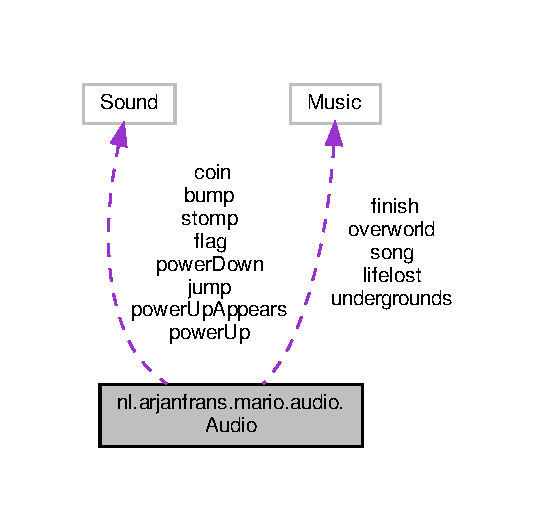
\includegraphics[width=258pt]{classnl_1_1arjanfrans_1_1mario_1_1audio_1_1Audio__coll__graph}
\end{center}
\end{figure}
\subsection*{Static Public Member Functions}
\begin{DoxyCompactItemize}
\item 
static void \hyperlink{classnl_1_1arjanfrans_1_1mario_1_1audio_1_1Audio_aaadf4a3f91b5908a1e73c7dab8f15c00}{play\+Song} (String name, boolean looping)
\begin{DoxyCompactList}\small\item\em A method meant to play a song on loop depending on the state of the game. \end{DoxyCompactList}\item 
static Music \hyperlink{classnl_1_1arjanfrans_1_1mario_1_1audio_1_1Audio_adb8068907967606c1f2cf680e04afaa3}{get\+Song} ()
\begin{DoxyCompactList}\small\item\em A method meant to play a song on loop depending on the state of the game. \end{DoxyCompactList}\item 
\mbox{\Hypertarget{classnl_1_1arjanfrans_1_1mario_1_1audio_1_1Audio_a47a221faf6b2c56402c95720bf46ad70}\label{classnl_1_1arjanfrans_1_1mario_1_1audio_1_1Audio_a47a221faf6b2c56402c95720bf46ad70}} 
static void \hyperlink{classnl_1_1arjanfrans_1_1mario_1_1audio_1_1Audio_a47a221faf6b2c56402c95720bf46ad70}{stop\+Song} ()
\begin{DoxyCompactList}\small\item\em A method meant to stop the current song instance variable from playing. \end{DoxyCompactList}\item 
\mbox{\Hypertarget{classnl_1_1arjanfrans_1_1mario_1_1audio_1_1Audio_ae9e32f01c3273c8d0e30a109602af1d4}\label{classnl_1_1arjanfrans_1_1mario_1_1audio_1_1Audio_ae9e32f01c3273c8d0e30a109602af1d4}} 
static void \hyperlink{classnl_1_1arjanfrans_1_1mario_1_1audio_1_1Audio_ae9e32f01c3273c8d0e30a109602af1d4}{dispose} ()
\begin{DoxyCompactList}\small\item\em A method meant to dispose of all the music files. \end{DoxyCompactList}\end{DoxyCompactItemize}
\subsection*{Static Public Attributes}
\begin{DoxyCompactItemize}
\item 
\mbox{\Hypertarget{classnl_1_1arjanfrans_1_1mario_1_1audio_1_1Audio_ac745382e99ecaa230981b95922a343b0}\label{classnl_1_1arjanfrans_1_1mario_1_1audio_1_1Audio_ac745382e99ecaa230981b95922a343b0}} 
static Sound {\bfseries jump} = Gdx.\+audio.\+new\+Sound(Gdx.\+files.\+internal(\char`\"{}data/audio/sfx/sounds/jump-\/small.\+wav\char`\"{}))
\item 
\mbox{\Hypertarget{classnl_1_1arjanfrans_1_1mario_1_1audio_1_1Audio_ad1c5e4b12abbe4a7ac54e604a66ca938}\label{classnl_1_1arjanfrans_1_1mario_1_1audio_1_1Audio_ad1c5e4b12abbe4a7ac54e604a66ca938}} 
static Sound {\bfseries stomp} = Gdx.\+audio.\+new\+Sound(Gdx.\+files.\+internal(\char`\"{}data/audio/sfx/sounds/stomp.\+wav\char`\"{}))
\item 
\mbox{\Hypertarget{classnl_1_1arjanfrans_1_1mario_1_1audio_1_1Audio_aaad87b915c08807251c2499acfee7aea}\label{classnl_1_1arjanfrans_1_1mario_1_1audio_1_1Audio_aaad87b915c08807251c2499acfee7aea}} 
static Sound {\bfseries bump} = Gdx.\+audio.\+new\+Sound(Gdx.\+files.\+internal(\char`\"{}data/audio/sfx/sounds/bump.\+wav\char`\"{}))
\item 
\mbox{\Hypertarget{classnl_1_1arjanfrans_1_1mario_1_1audio_1_1Audio_a9e01185b0b590c94ee5a7f688a4089ee}\label{classnl_1_1arjanfrans_1_1mario_1_1audio_1_1Audio_a9e01185b0b590c94ee5a7f688a4089ee}} 
static Sound {\bfseries flag} = Gdx.\+audio.\+new\+Sound(Gdx.\+files.\+internal(\char`\"{}data/audio/sfx/sounds/flagpole.\+wav\char`\"{}))
\item 
\mbox{\Hypertarget{classnl_1_1arjanfrans_1_1mario_1_1audio_1_1Audio_a018223f086974df36bd1cb093311bf24}\label{classnl_1_1arjanfrans_1_1mario_1_1audio_1_1Audio_a018223f086974df36bd1cb093311bf24}} 
static Sound {\bfseries power\+Down} = Gdx.\+audio.\+new\+Sound(Gdx.\+files.\+internal(\char`\"{}data/audio/sfx/sounds/pipeandpowerdown.\+wav\char`\"{}))
\item 
\mbox{\Hypertarget{classnl_1_1arjanfrans_1_1mario_1_1audio_1_1Audio_adfd739566cd06b276841f91012724dc6}\label{classnl_1_1arjanfrans_1_1mario_1_1audio_1_1Audio_adfd739566cd06b276841f91012724dc6}} 
static Sound {\bfseries power\+Up} = Gdx.\+audio.\+new\+Sound(Gdx.\+files.\+internal(\char`\"{}data/audio/sfx/sounds/powerup.\+wav\char`\"{}))
\item 
\mbox{\Hypertarget{classnl_1_1arjanfrans_1_1mario_1_1audio_1_1Audio_a862fdb3e8e6904c3f2bc62692bffa95b}\label{classnl_1_1arjanfrans_1_1mario_1_1audio_1_1Audio_a862fdb3e8e6904c3f2bc62692bffa95b}} 
static Sound {\bfseries power\+Up\+Appears} = Gdx.\+audio.\+new\+Sound(Gdx.\+files.\+internal(\char`\"{}data/audio/sfx/sounds/powerup\+\_\+appears.\+wav\char`\"{}))
\item 
\mbox{\Hypertarget{classnl_1_1arjanfrans_1_1mario_1_1audio_1_1Audio_a25432d77021bb323bd2230a57b4859ef}\label{classnl_1_1arjanfrans_1_1mario_1_1audio_1_1Audio_a25432d77021bb323bd2230a57b4859ef}} 
static Sound {\bfseries coin} = Gdx.\+audio.\+new\+Sound(Gdx.\+files.\+internal(\char`\"{}data/audio/sfx/sounds/coin.\+wav\char`\"{}))
\item 
\mbox{\Hypertarget{classnl_1_1arjanfrans_1_1mario_1_1audio_1_1Audio_a898dcecd8d3a7dc83e3674b5f0f7d555}\label{classnl_1_1arjanfrans_1_1mario_1_1audio_1_1Audio_a898dcecd8d3a7dc83e3674b5f0f7d555}} 
static String {\bfseries current\+Song} = \char`\"{}\char`\"{}
\end{DoxyCompactItemize}
\subsection*{Static Private Attributes}
\begin{DoxyCompactItemize}
\item 
\mbox{\Hypertarget{classnl_1_1arjanfrans_1_1mario_1_1audio_1_1Audio_a972d82e5a10d253ba0e5193c0bd154c4}\label{classnl_1_1arjanfrans_1_1mario_1_1audio_1_1Audio_a972d82e5a10d253ba0e5193c0bd154c4}} 
static Music {\bfseries overworld} = Gdx.\+audio.\+new\+Music(Gdx.\+files.\+internal(\char`\"{}data/audio/soundtracks/Overworld.\+ogg\char`\"{}))
\item 
\mbox{\Hypertarget{classnl_1_1arjanfrans_1_1mario_1_1audio_1_1Audio_a6a7589e0741964c5e4bbf9513d999c87}\label{classnl_1_1arjanfrans_1_1mario_1_1audio_1_1Audio_a6a7589e0741964c5e4bbf9513d999c87}} 
static Music {\bfseries undergrounds} = Gdx.\+audio.\+new\+Music(Gdx.\+files.\+internal(\char`\"{}data/audio/soundtracks/Undergrounds.\+ogg\char`\"{}))
\item 
\mbox{\Hypertarget{classnl_1_1arjanfrans_1_1mario_1_1audio_1_1Audio_afd25ef719ffb4c864c2042ff664f0c57}\label{classnl_1_1arjanfrans_1_1mario_1_1audio_1_1Audio_afd25ef719ffb4c864c2042ff664f0c57}} 
static Music {\bfseries lifelost} = Gdx.\+audio.\+new\+Music(Gdx.\+files.\+internal(\char`\"{}data/audio/soundtracks/Life Lost.\+ogg\char`\"{}))
\item 
\mbox{\Hypertarget{classnl_1_1arjanfrans_1_1mario_1_1audio_1_1Audio_a8fc0b3722de97cc32b3ae3e906df399c}\label{classnl_1_1arjanfrans_1_1mario_1_1audio_1_1Audio_a8fc0b3722de97cc32b3ae3e906df399c}} 
static Music {\bfseries finish} = Gdx.\+audio.\+new\+Music(Gdx.\+files.\+internal(\char`\"{}data/audio/soundtracks/Course Clear.\+ogg\char`\"{}))
\item 
\mbox{\Hypertarget{classnl_1_1arjanfrans_1_1mario_1_1audio_1_1Audio_a93c280ab77245f3d66d3d8b90fc189c7}\label{classnl_1_1arjanfrans_1_1mario_1_1audio_1_1Audio_a93c280ab77245f3d66d3d8b90fc189c7}} 
static Music {\bfseries song}
\end{DoxyCompactItemize}


\subsection{Detailed Description}
This is a class that implements the audio in the game. 

\subsection{Member Function Documentation}
\mbox{\Hypertarget{classnl_1_1arjanfrans_1_1mario_1_1audio_1_1Audio_adb8068907967606c1f2cf680e04afaa3}\label{classnl_1_1arjanfrans_1_1mario_1_1audio_1_1Audio_adb8068907967606c1f2cf680e04afaa3}} 
\index{nl\+::arjanfrans\+::mario\+::audio\+::\+Audio@{nl\+::arjanfrans\+::mario\+::audio\+::\+Audio}!get\+Song@{get\+Song}}
\index{get\+Song@{get\+Song}!nl\+::arjanfrans\+::mario\+::audio\+::\+Audio@{nl\+::arjanfrans\+::mario\+::audio\+::\+Audio}}
\subsubsection{\texorpdfstring{get\+Song()}{getSong()}}
{\footnotesize\ttfamily static Music nl.\+arjanfrans.\+mario.\+audio.\+Audio.\+get\+Song (\begin{DoxyParamCaption}{ }\end{DoxyParamCaption})\hspace{0.3cm}{\ttfamily [static]}}



A method meant to play a song on loop depending on the state of the game. 

\begin{DoxyReturn}{Returns}
a Music object, the current value of the global song variable. 
\end{DoxyReturn}
\mbox{\Hypertarget{classnl_1_1arjanfrans_1_1mario_1_1audio_1_1Audio_aaadf4a3f91b5908a1e73c7dab8f15c00}\label{classnl_1_1arjanfrans_1_1mario_1_1audio_1_1Audio_aaadf4a3f91b5908a1e73c7dab8f15c00}} 
\index{nl\+::arjanfrans\+::mario\+::audio\+::\+Audio@{nl\+::arjanfrans\+::mario\+::audio\+::\+Audio}!play\+Song@{play\+Song}}
\index{play\+Song@{play\+Song}!nl\+::arjanfrans\+::mario\+::audio\+::\+Audio@{nl\+::arjanfrans\+::mario\+::audio\+::\+Audio}}
\subsubsection{\texorpdfstring{play\+Song()}{playSong()}}
{\footnotesize\ttfamily static void nl.\+arjanfrans.\+mario.\+audio.\+Audio.\+play\+Song (\begin{DoxyParamCaption}\item[{String}]{name,  }\item[{boolean}]{looping }\end{DoxyParamCaption})\hspace{0.3cm}{\ttfamily [static]}}



A method meant to play a song on loop depending on the state of the game. 


\begin{DoxyParams}{Parameters}
{\em name} & -\/ the name of the song (based on the state of the game). \\
\hline
{\em looping} & -\/ a boolean meant to indicate whether the song is looping or not. \\
\hline
\end{DoxyParams}


The documentation for this class was generated from the following file\+:\begin{DoxyCompactItemize}
\item 
core/src/nl/arjanfrans/mario/audio/Audio.\+java\end{DoxyCompactItemize}

\hypertarget{classnl_1_1arjanfrans_1_1mario_1_1model_1_1Brick}{}\section{nl.\+arjanfrans.\+mario.\+model.\+Brick Class Reference}
\label{classnl_1_1arjanfrans_1_1mario_1_1model_1_1Brick}\index{nl.\+arjanfrans.\+mario.\+model.\+Brick@{nl.\+arjanfrans.\+mario.\+model.\+Brick}}


This class is the class meant to model the bricks in the game.  




Inheritance diagram for nl.\+arjanfrans.\+mario.\+model.\+Brick\+:\nopagebreak
\begin{figure}[H]
\begin{center}
\leavevmode
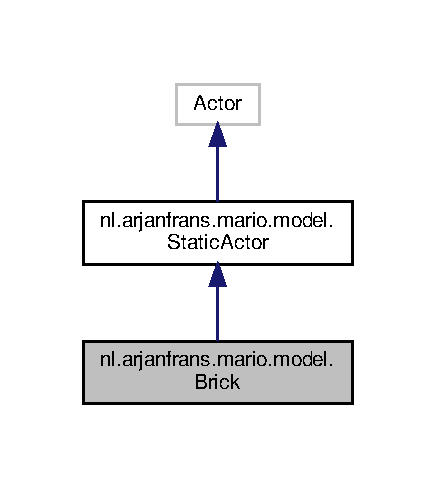
\includegraphics[width=209pt]{classnl_1_1arjanfrans_1_1mario_1_1model_1_1Brick__inherit__graph}
\end{center}
\end{figure}


Collaboration diagram for nl.\+arjanfrans.\+mario.\+model.\+Brick\+:
\nopagebreak
\begin{figure}[H]
\begin{center}
\leavevmode
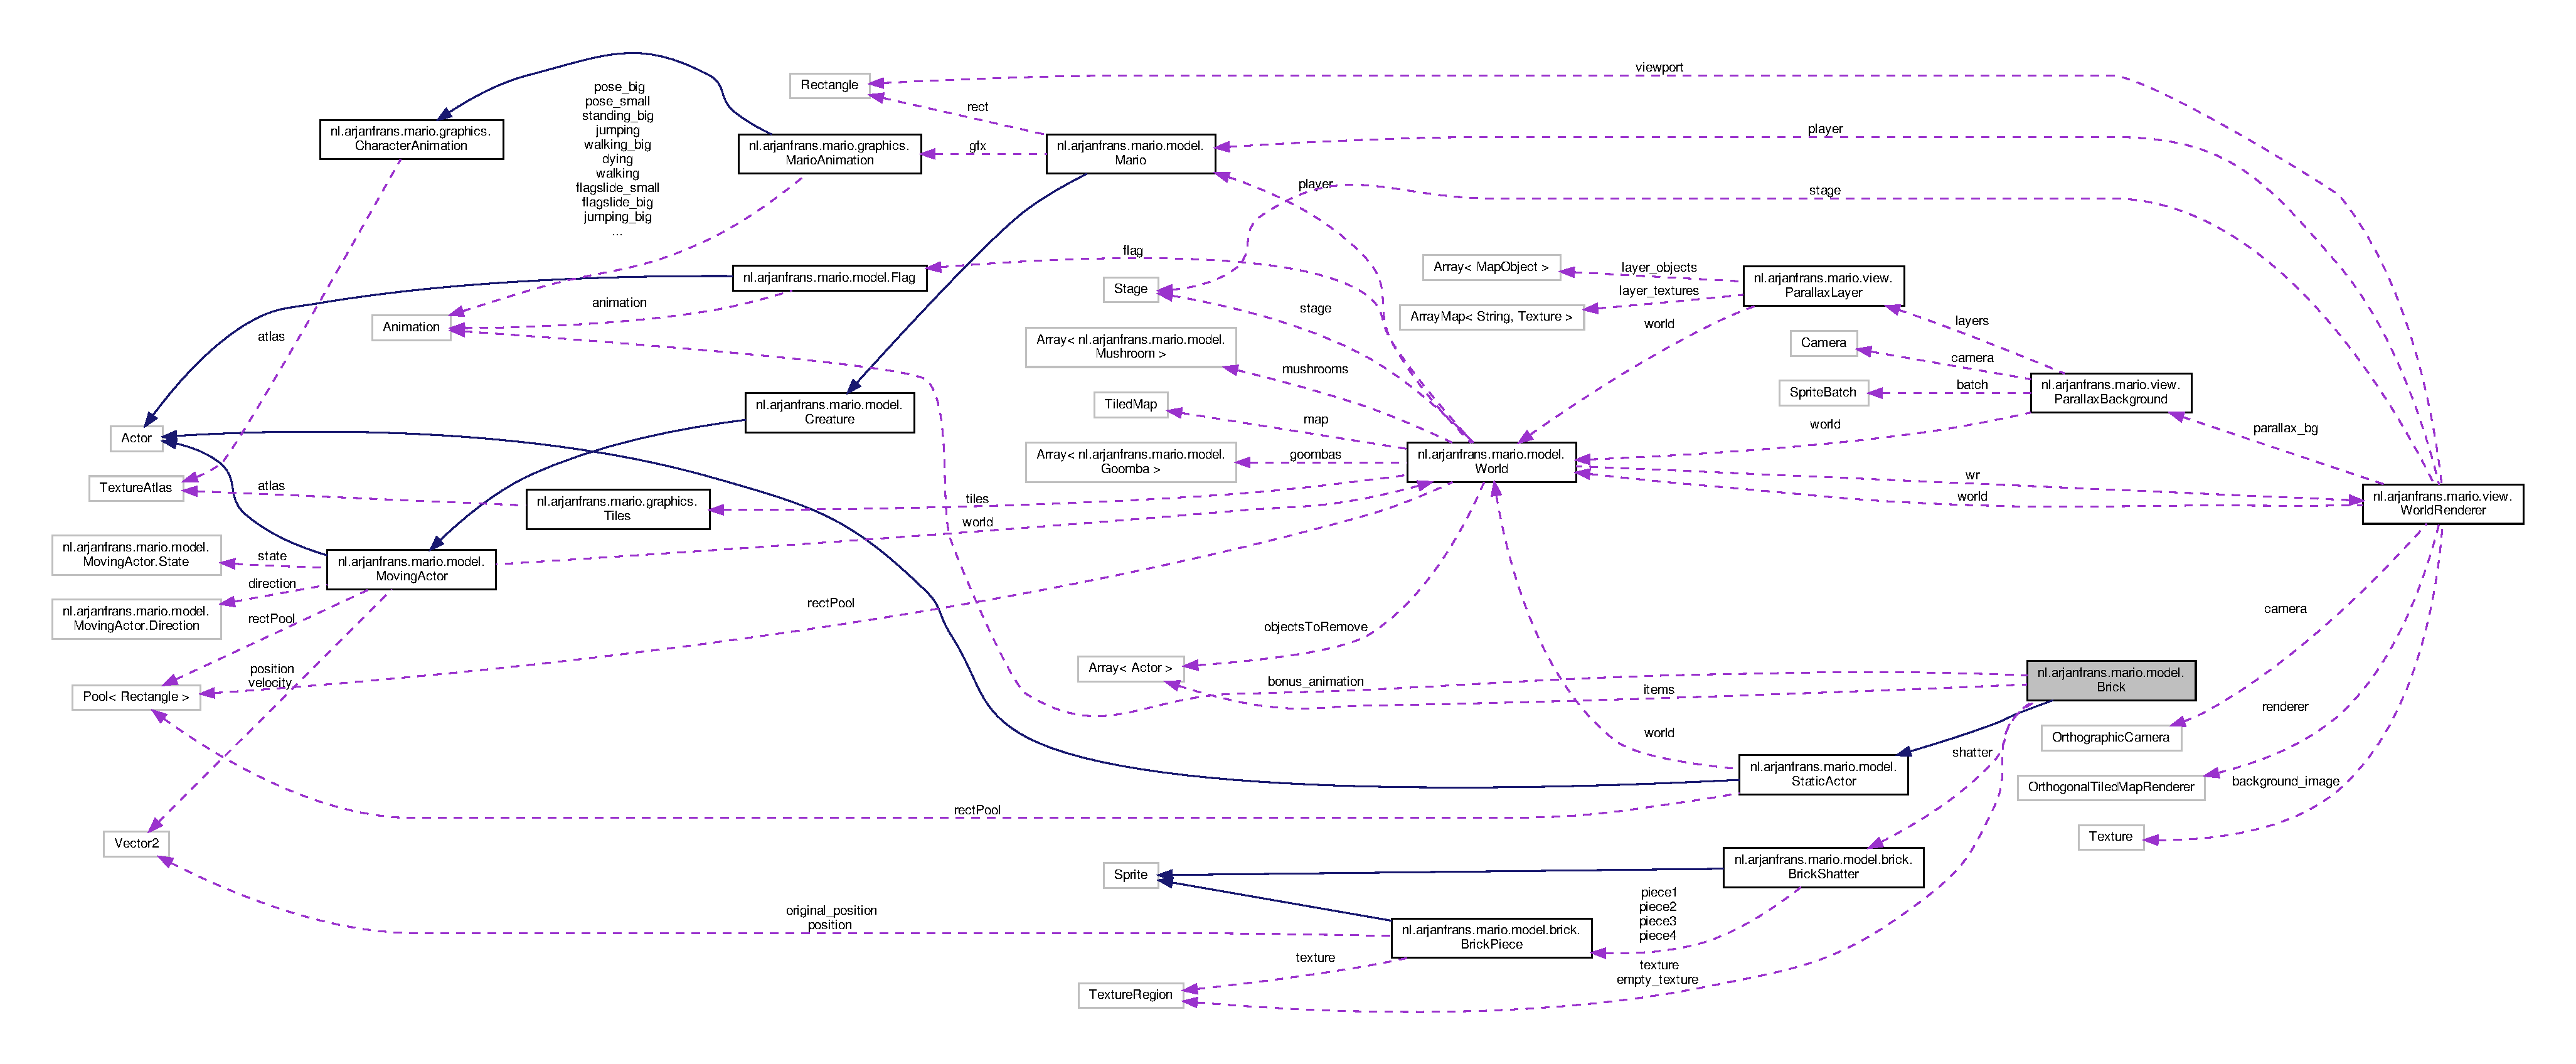
\includegraphics[width=350pt]{classnl_1_1arjanfrans_1_1mario_1_1model_1_1Brick__coll__graph}
\end{center}
\end{figure}
\subsection*{Public Member Functions}
\begin{DoxyCompactItemize}
\item 
\hyperlink{classnl_1_1arjanfrans_1_1mario_1_1model_1_1Brick_addfb506d6f243693b69d579b2cedb3ec}{Brick} (\hyperlink{classnl_1_1arjanfrans_1_1mario_1_1model_1_1World}{World} world, float x, float y, String color, boolean bonus, boolean destructable)
\begin{DoxyCompactList}\small\item\em Constructor method. \end{DoxyCompactList}\item 
void \hyperlink{classnl_1_1arjanfrans_1_1mario_1_1model_1_1Brick_a04b6eece7156ca21f139a20809220f17}{act} (float delta)
\begin{DoxyCompactList}\small\item\em This method updates the actor based on time. \end{DoxyCompactList}\item 
void \hyperlink{classnl_1_1arjanfrans_1_1mario_1_1model_1_1Brick_a92e1021bfa260049d650dc962874b19a}{draw} (Batch batch, float parent\+Alpha)
\begin{DoxyCompactList}\small\item\em This method updates the actor based on time. \end{DoxyCompactList}\item 
void \hyperlink{classnl_1_1arjanfrans_1_1mario_1_1model_1_1Brick_aeca0f5bee7ddc1377fd85e60e8341590}{hit} (int mario\+\_\+level)
\begin{DoxyCompactList}\small\item\em This method models the behaviour when the brick has been hit. \end{DoxyCompactList}\item 
float \hyperlink{classnl_1_1arjanfrans_1_1mario_1_1model_1_1Brick_a423a5d8853e99442315e102408f3e0ec}{getX} ()
\begin{DoxyCompactList}\small\item\em This method gets the x coordinate of the brick. \end{DoxyCompactList}\item 
float \hyperlink{classnl_1_1arjanfrans_1_1mario_1_1model_1_1Brick_afc049458a63d92b001328afe8714c2f8}{getY} ()
\begin{DoxyCompactList}\small\item\em This method gets the y coordinate of the brick. \end{DoxyCompactList}\item 
Array$<$ Actor $>$ \hyperlink{classnl_1_1arjanfrans_1_1mario_1_1model_1_1Brick_ab7c75746c482b7e43dc22937cf100624}{get\+Items} ()
\begin{DoxyCompactList}\small\item\em This method gets items located inside the brick. \end{DoxyCompactList}\item 
Actor \hyperlink{classnl_1_1arjanfrans_1_1mario_1_1model_1_1Brick_aae68460b9c629b1bc3b81bbcdc168554}{pop\+Item} ()
\begin{DoxyCompactList}\small\item\em This method pops the top item located inside the brick. \end{DoxyCompactList}\item 
void \hyperlink{classnl_1_1arjanfrans_1_1mario_1_1model_1_1Brick_adb38a0e3d30ff07d38ad8d4549642afd}{add\+Item} (Actor item)
\begin{DoxyCompactList}\small\item\em This method adds an item to the arrat of items located inside the brick. \end{DoxyCompactList}\end{DoxyCompactItemize}
\subsection*{Private Member Functions}
\begin{DoxyCompactItemize}
\item 
\mbox{\Hypertarget{classnl_1_1arjanfrans_1_1mario_1_1model_1_1Brick_a29d45291a530d66038ac80b41d3b7da7}\label{classnl_1_1arjanfrans_1_1mario_1_1model_1_1Brick_a29d45291a530d66038ac80b41d3b7da7}} 
void \hyperlink{classnl_1_1arjanfrans_1_1mario_1_1model_1_1Brick_a29d45291a530d66038ac80b41d3b7da7}{shatter} ()
\begin{DoxyCompactList}\small\item\em Shatters the brick into pieces. \end{DoxyCompactList}\end{DoxyCompactItemize}
\subsection*{Private Attributes}
\begin{DoxyCompactItemize}
\item 
\mbox{\Hypertarget{classnl_1_1arjanfrans_1_1mario_1_1model_1_1Brick_a0e80b3217db810a3562ad29e719c569b}\label{classnl_1_1arjanfrans_1_1mario_1_1model_1_1Brick_a0e80b3217db810a3562ad29e719c569b}} 
Texture\+Region {\bfseries texture}
\item 
\mbox{\Hypertarget{classnl_1_1arjanfrans_1_1mario_1_1model_1_1Brick_a2a317d6a79b1e5d769b3615a8ae9901c}\label{classnl_1_1arjanfrans_1_1mario_1_1model_1_1Brick_a2a317d6a79b1e5d769b3615a8ae9901c}} 
Texture\+Region {\bfseries empty\+\_\+texture}
\item 
\mbox{\Hypertarget{classnl_1_1arjanfrans_1_1mario_1_1model_1_1Brick_ade3c2d8745901c5f36760c22d29ed504}\label{classnl_1_1arjanfrans_1_1mario_1_1model_1_1Brick_ade3c2d8745901c5f36760c22d29ed504}} 
float {\bfseries state\+Time}
\item 
\mbox{\Hypertarget{classnl_1_1arjanfrans_1_1mario_1_1model_1_1Brick_a4be7c1748a61eef89a9c3fa250bd086d}\label{classnl_1_1arjanfrans_1_1mario_1_1model_1_1Brick_a4be7c1748a61eef89a9c3fa250bd086d}} 
int {\bfseries hitcount} = 0
\item 
\mbox{\Hypertarget{classnl_1_1arjanfrans_1_1mario_1_1model_1_1Brick_a97ffa6b04b51f21b5c1f49c0f4553cf0}\label{classnl_1_1arjanfrans_1_1mario_1_1model_1_1Brick_a97ffa6b04b51f21b5c1f49c0f4553cf0}} 
int {\bfseries maxhits} = 1
\item 
\mbox{\Hypertarget{classnl_1_1arjanfrans_1_1mario_1_1model_1_1Brick_a1db87783d4ee6d14be257d6f1f274fe9}\label{classnl_1_1arjanfrans_1_1mario_1_1model_1_1Brick_a1db87783d4ee6d14be257d6f1f274fe9}} 
boolean {\bfseries destructable}
\item 
\mbox{\Hypertarget{classnl_1_1arjanfrans_1_1mario_1_1model_1_1Brick_ab41704c5f4769eea1a572deb6cc23e50}\label{classnl_1_1arjanfrans_1_1mario_1_1model_1_1Brick_ab41704c5f4769eea1a572deb6cc23e50}} 
Array$<$ Actor $>$ {\bfseries items}
\item 
\mbox{\Hypertarget{classnl_1_1arjanfrans_1_1mario_1_1model_1_1Brick_a41b6318887cb6ea970c78fa90a6d951b}\label{classnl_1_1arjanfrans_1_1mario_1_1model_1_1Brick_a41b6318887cb6ea970c78fa90a6d951b}} 
boolean {\bfseries bonus}
\item 
\mbox{\Hypertarget{classnl_1_1arjanfrans_1_1mario_1_1model_1_1Brick_ada311ec6c5707737328010f839fc5f8a}\label{classnl_1_1arjanfrans_1_1mario_1_1model_1_1Brick_ada311ec6c5707737328010f839fc5f8a}} 
\hyperlink{classnl_1_1arjanfrans_1_1mario_1_1model_1_1brick_1_1BrickShatter}{Brick\+Shatter} {\bfseries shatter}
\end{DoxyCompactItemize}
\subsection*{Static Private Attributes}
\begin{DoxyCompactItemize}
\item 
\mbox{\Hypertarget{classnl_1_1arjanfrans_1_1mario_1_1model_1_1Brick_a3ccb1a16df0627a2a15ef1972f950f51}\label{classnl_1_1arjanfrans_1_1mario_1_1model_1_1Brick_a3ccb1a16df0627a2a15ef1972f950f51}} 
static Animation {\bfseries bonus\+\_\+animation}
\end{DoxyCompactItemize}
\subsection*{Additional Inherited Members}


\subsection{Detailed Description}
This class is the class meant to model the bricks in the game. 

\subsection{Constructor \& Destructor Documentation}
\mbox{\Hypertarget{classnl_1_1arjanfrans_1_1mario_1_1model_1_1Brick_addfb506d6f243693b69d579b2cedb3ec}\label{classnl_1_1arjanfrans_1_1mario_1_1model_1_1Brick_addfb506d6f243693b69d579b2cedb3ec}} 
\index{nl\+::arjanfrans\+::mario\+::model\+::\+Brick@{nl\+::arjanfrans\+::mario\+::model\+::\+Brick}!Brick@{Brick}}
\index{Brick@{Brick}!nl\+::arjanfrans\+::mario\+::model\+::\+Brick@{nl\+::arjanfrans\+::mario\+::model\+::\+Brick}}
\subsubsection{\texorpdfstring{Brick()}{Brick()}}
{\footnotesize\ttfamily nl.\+arjanfrans.\+mario.\+model.\+Brick.\+Brick (\begin{DoxyParamCaption}\item[{\hyperlink{classnl_1_1arjanfrans_1_1mario_1_1model_1_1World}{World}}]{world,  }\item[{float}]{x,  }\item[{float}]{y,  }\item[{String}]{color,  }\item[{boolean}]{bonus,  }\item[{boolean}]{destructable }\end{DoxyParamCaption})}



Constructor method. 

Method which initializes an instance of \hyperlink{classnl_1_1arjanfrans_1_1mario_1_1model_1_1Brick}{Brick}. 
\begin{DoxyParams}{Parameters}
{\em world} & -\/ \hyperlink{classnl_1_1arjanfrans_1_1mario_1_1model_1_1World}{World} object which defines which game instance the brick exists in. \\
\hline
{\em x} & -\/ The initial x coordinate for the brick. \\
\hline
{\em y} & -\/ The initial y coordinate for the creature. \\
\hline
{\em color} & -\/ a string representing the brick\textquotesingle{}s color. \\
\hline
{\em bonus} & -\/ a boolean indicating the existence of a bonus \\
\hline
{\em destructable} & -\/ a boolean indicating the ability to destroy a brick \\
\hline
\end{DoxyParams}
\begin{DoxyReturn}{Returns}
An instance of \hyperlink{classnl_1_1arjanfrans_1_1mario_1_1model_1_1Brick}{Brick} 
\end{DoxyReturn}


\subsection{Member Function Documentation}
\mbox{\Hypertarget{classnl_1_1arjanfrans_1_1mario_1_1model_1_1Brick_a04b6eece7156ca21f139a20809220f17}\label{classnl_1_1arjanfrans_1_1mario_1_1model_1_1Brick_a04b6eece7156ca21f139a20809220f17}} 
\index{nl\+::arjanfrans\+::mario\+::model\+::\+Brick@{nl\+::arjanfrans\+::mario\+::model\+::\+Brick}!act@{act}}
\index{act@{act}!nl\+::arjanfrans\+::mario\+::model\+::\+Brick@{nl\+::arjanfrans\+::mario\+::model\+::\+Brick}}
\subsubsection{\texorpdfstring{act()}{act()}}
{\footnotesize\ttfamily void nl.\+arjanfrans.\+mario.\+model.\+Brick.\+act (\begin{DoxyParamCaption}\item[{float}]{delta }\end{DoxyParamCaption})}



This method updates the actor based on time. 


\begin{DoxyParams}{Parameters}
{\em delta} & -\/ Time in seconds since the last frame. \\
\hline
\end{DoxyParams}
\mbox{\Hypertarget{classnl_1_1arjanfrans_1_1mario_1_1model_1_1Brick_adb38a0e3d30ff07d38ad8d4549642afd}\label{classnl_1_1arjanfrans_1_1mario_1_1model_1_1Brick_adb38a0e3d30ff07d38ad8d4549642afd}} 
\index{nl\+::arjanfrans\+::mario\+::model\+::\+Brick@{nl\+::arjanfrans\+::mario\+::model\+::\+Brick}!add\+Item@{add\+Item}}
\index{add\+Item@{add\+Item}!nl\+::arjanfrans\+::mario\+::model\+::\+Brick@{nl\+::arjanfrans\+::mario\+::model\+::\+Brick}}
\subsubsection{\texorpdfstring{add\+Item()}{addItem()}}
{\footnotesize\ttfamily void nl.\+arjanfrans.\+mario.\+model.\+Brick.\+add\+Item (\begin{DoxyParamCaption}\item[{Actor}]{item }\end{DoxyParamCaption})}



This method adds an item to the arrat of items located inside the brick. 


\begin{DoxyParams}{Parameters}
{\em item} & -\/ an Actor object. \\
\hline
\end{DoxyParams}
\mbox{\Hypertarget{classnl_1_1arjanfrans_1_1mario_1_1model_1_1Brick_a92e1021bfa260049d650dc962874b19a}\label{classnl_1_1arjanfrans_1_1mario_1_1model_1_1Brick_a92e1021bfa260049d650dc962874b19a}} 
\index{nl\+::arjanfrans\+::mario\+::model\+::\+Brick@{nl\+::arjanfrans\+::mario\+::model\+::\+Brick}!draw@{draw}}
\index{draw@{draw}!nl\+::arjanfrans\+::mario\+::model\+::\+Brick@{nl\+::arjanfrans\+::mario\+::model\+::\+Brick}}
\subsubsection{\texorpdfstring{draw()}{draw()}}
{\footnotesize\ttfamily void nl.\+arjanfrans.\+mario.\+model.\+Brick.\+draw (\begin{DoxyParamCaption}\item[{Batch}]{batch,  }\item[{float}]{parent\+Alpha }\end{DoxyParamCaption})}



This method updates the actor based on time. 


\begin{DoxyParams}{Parameters}
{\em parent\+Alpha} & -\/ The parent alpha, to be multiplied with this actor\textquotesingle{}s alpha, allowing the parent\textquotesingle{}s alpha to affect all children. \\
\hline
{\em batch} & -\/ an object used to draw 2D rectangles that reference a texture (region). \\
\hline
\end{DoxyParams}
\mbox{\Hypertarget{classnl_1_1arjanfrans_1_1mario_1_1model_1_1Brick_ab7c75746c482b7e43dc22937cf100624}\label{classnl_1_1arjanfrans_1_1mario_1_1model_1_1Brick_ab7c75746c482b7e43dc22937cf100624}} 
\index{nl\+::arjanfrans\+::mario\+::model\+::\+Brick@{nl\+::arjanfrans\+::mario\+::model\+::\+Brick}!get\+Items@{get\+Items}}
\index{get\+Items@{get\+Items}!nl\+::arjanfrans\+::mario\+::model\+::\+Brick@{nl\+::arjanfrans\+::mario\+::model\+::\+Brick}}
\subsubsection{\texorpdfstring{get\+Items()}{getItems()}}
{\footnotesize\ttfamily Array$<$Actor$>$ nl.\+arjanfrans.\+mario.\+model.\+Brick.\+get\+Items (\begin{DoxyParamCaption}{ }\end{DoxyParamCaption})}



This method gets items located inside the brick. 

\begin{DoxyReturn}{Returns}
an array of Actor objects. 
\end{DoxyReturn}
\mbox{\Hypertarget{classnl_1_1arjanfrans_1_1mario_1_1model_1_1Brick_a423a5d8853e99442315e102408f3e0ec}\label{classnl_1_1arjanfrans_1_1mario_1_1model_1_1Brick_a423a5d8853e99442315e102408f3e0ec}} 
\index{nl\+::arjanfrans\+::mario\+::model\+::\+Brick@{nl\+::arjanfrans\+::mario\+::model\+::\+Brick}!getX@{getX}}
\index{getX@{getX}!nl\+::arjanfrans\+::mario\+::model\+::\+Brick@{nl\+::arjanfrans\+::mario\+::model\+::\+Brick}}
\subsubsection{\texorpdfstring{get\+X()}{getX()}}
{\footnotesize\ttfamily float nl.\+arjanfrans.\+mario.\+model.\+Brick.\+getX (\begin{DoxyParamCaption}{ }\end{DoxyParamCaption})}



This method gets the x coordinate of the brick. 

\begin{DoxyReturn}{Returns}
a float representing the y coordinate. 
\end{DoxyReturn}
\mbox{\Hypertarget{classnl_1_1arjanfrans_1_1mario_1_1model_1_1Brick_afc049458a63d92b001328afe8714c2f8}\label{classnl_1_1arjanfrans_1_1mario_1_1model_1_1Brick_afc049458a63d92b001328afe8714c2f8}} 
\index{nl\+::arjanfrans\+::mario\+::model\+::\+Brick@{nl\+::arjanfrans\+::mario\+::model\+::\+Brick}!getY@{getY}}
\index{getY@{getY}!nl\+::arjanfrans\+::mario\+::model\+::\+Brick@{nl\+::arjanfrans\+::mario\+::model\+::\+Brick}}
\subsubsection{\texorpdfstring{get\+Y()}{getY()}}
{\footnotesize\ttfamily float nl.\+arjanfrans.\+mario.\+model.\+Brick.\+getY (\begin{DoxyParamCaption}{ }\end{DoxyParamCaption})}



This method gets the y coordinate of the brick. 

\begin{DoxyReturn}{Returns}
a float representing the y coordinate. 
\end{DoxyReturn}
\mbox{\Hypertarget{classnl_1_1arjanfrans_1_1mario_1_1model_1_1Brick_aeca0f5bee7ddc1377fd85e60e8341590}\label{classnl_1_1arjanfrans_1_1mario_1_1model_1_1Brick_aeca0f5bee7ddc1377fd85e60e8341590}} 
\index{nl\+::arjanfrans\+::mario\+::model\+::\+Brick@{nl\+::arjanfrans\+::mario\+::model\+::\+Brick}!hit@{hit}}
\index{hit@{hit}!nl\+::arjanfrans\+::mario\+::model\+::\+Brick@{nl\+::arjanfrans\+::mario\+::model\+::\+Brick}}
\subsubsection{\texorpdfstring{hit()}{hit()}}
{\footnotesize\ttfamily void nl.\+arjanfrans.\+mario.\+model.\+Brick.\+hit (\begin{DoxyParamCaption}\item[{int}]{mario\+\_\+level }\end{DoxyParamCaption})}



This method models the behaviour when the brick has been hit. 


\begin{DoxyParams}{Parameters}
{\em mario\+\_\+level} & -\/ an integer indicating the size of \hyperlink{classnl_1_1arjanfrans_1_1mario_1_1model_1_1Mario}{Mario}. \\
\hline
\end{DoxyParams}
\mbox{\Hypertarget{classnl_1_1arjanfrans_1_1mario_1_1model_1_1Brick_aae68460b9c629b1bc3b81bbcdc168554}\label{classnl_1_1arjanfrans_1_1mario_1_1model_1_1Brick_aae68460b9c629b1bc3b81bbcdc168554}} 
\index{nl\+::arjanfrans\+::mario\+::model\+::\+Brick@{nl\+::arjanfrans\+::mario\+::model\+::\+Brick}!pop\+Item@{pop\+Item}}
\index{pop\+Item@{pop\+Item}!nl\+::arjanfrans\+::mario\+::model\+::\+Brick@{nl\+::arjanfrans\+::mario\+::model\+::\+Brick}}
\subsubsection{\texorpdfstring{pop\+Item()}{popItem()}}
{\footnotesize\ttfamily Actor nl.\+arjanfrans.\+mario.\+model.\+Brick.\+pop\+Item (\begin{DoxyParamCaption}{ }\end{DoxyParamCaption})}



This method pops the top item located inside the brick. 

\begin{DoxyReturn}{Returns}
an Actor object. 
\end{DoxyReturn}


The documentation for this class was generated from the following file\+:\begin{DoxyCompactItemize}
\item 
core/src/nl/arjanfrans/mario/model/Brick.\+java\end{DoxyCompactItemize}

\hypertarget{classnl_1_1arjanfrans_1_1mario_1_1model_1_1brick_1_1BrickPiece}{}\section{nl.\+arjanfrans.\+mario.\+model.\+brick.\+Brick\+Piece Class Reference}
\label{classnl_1_1arjanfrans_1_1mario_1_1model_1_1brick_1_1BrickPiece}\index{nl.\+arjanfrans.\+mario.\+model.\+brick.\+Brick\+Piece@{nl.\+arjanfrans.\+mario.\+model.\+brick.\+Brick\+Piece}}


This class is the class meant to model the pieces of the bricks in the game.  




Inheritance diagram for nl.\+arjanfrans.\+mario.\+model.\+brick.\+Brick\+Piece\+:\nopagebreak
\begin{figure}[H]
\begin{center}
\leavevmode
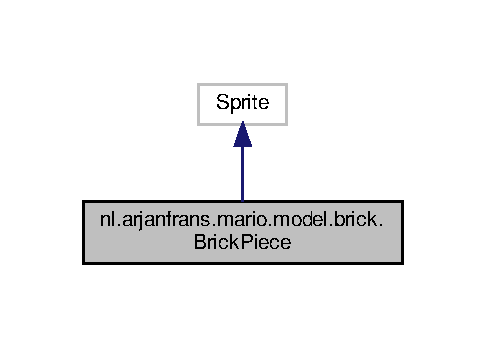
\includegraphics[width=233pt]{classnl_1_1arjanfrans_1_1mario_1_1model_1_1brick_1_1BrickPiece__inherit__graph}
\end{center}
\end{figure}


Collaboration diagram for nl.\+arjanfrans.\+mario.\+model.\+brick.\+Brick\+Piece\+:\nopagebreak
\begin{figure}[H]
\begin{center}
\leavevmode
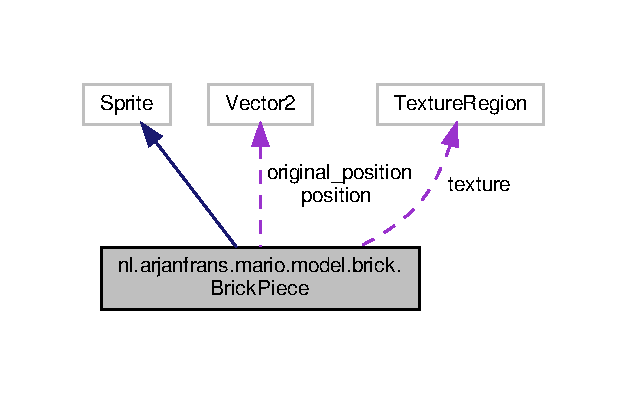
\includegraphics[width=301pt]{classnl_1_1arjanfrans_1_1mario_1_1model_1_1brick_1_1BrickPiece__coll__graph}
\end{center}
\end{figure}
\subsection*{Public Member Functions}
\begin{DoxyCompactItemize}
\item 
\hyperlink{classnl_1_1arjanfrans_1_1mario_1_1model_1_1brick_1_1BrickPiece_adb0ed3d619092f6f60661039261e6c2d}{Brick\+Piece} (float x, float y, int direction)
\begin{DoxyCompactList}\small\item\em Constructor method for \hyperlink{classnl_1_1arjanfrans_1_1mario_1_1model_1_1brick_1_1BrickPiece}{Brick\+Piece}. \end{DoxyCompactList}\item 
void \hyperlink{classnl_1_1arjanfrans_1_1mario_1_1model_1_1brick_1_1BrickPiece_ae299436fa0ff756fb83e3322afd545c6}{draw} (Batch batch)
\begin{DoxyCompactList}\small\item\em This is the method meant to draw a \hyperlink{classnl_1_1arjanfrans_1_1mario_1_1model_1_1brick_1_1BrickPiece}{Brick\+Piece}. \end{DoxyCompactList}\end{DoxyCompactItemize}
\subsection*{Private Attributes}
\begin{DoxyCompactItemize}
\item 
\mbox{\Hypertarget{classnl_1_1arjanfrans_1_1mario_1_1model_1_1brick_1_1BrickPiece_ad6528fab2d13e4f6158cd3a067ee3c49}\label{classnl_1_1arjanfrans_1_1mario_1_1model_1_1brick_1_1BrickPiece_ad6528fab2d13e4f6158cd3a067ee3c49}} 
Texture\+Region {\bfseries texture} = \hyperlink{classnl_1_1arjanfrans_1_1mario_1_1graphics_1_1Tiles_aec062c35528937ca08a65a3e5b120d91}{Tiles.\+get\+Tile8}(\char`\"{}brick\+\_\+piece\char`\"{})
\item 
\mbox{\Hypertarget{classnl_1_1arjanfrans_1_1mario_1_1model_1_1brick_1_1BrickPiece_ab3dbfcfa214e704bec8d2cdd3c74cc2a}\label{classnl_1_1arjanfrans_1_1mario_1_1model_1_1brick_1_1BrickPiece_ab3dbfcfa214e704bec8d2cdd3c74cc2a}} 
Vector2 {\bfseries position}
\item 
\mbox{\Hypertarget{classnl_1_1arjanfrans_1_1mario_1_1model_1_1brick_1_1BrickPiece_ac748ea115163f7627e601e1544776b18}\label{classnl_1_1arjanfrans_1_1mario_1_1model_1_1brick_1_1BrickPiece_ac748ea115163f7627e601e1544776b18}} 
Vector2 {\bfseries original\+\_\+position}
\item 
\mbox{\Hypertarget{classnl_1_1arjanfrans_1_1mario_1_1model_1_1brick_1_1BrickPiece_a264479cfcd3623e4545049c82625bde8}\label{classnl_1_1arjanfrans_1_1mario_1_1model_1_1brick_1_1BrickPiece_a264479cfcd3623e4545049c82625bde8}} 
float {\bfseries angle} = 0
\item 
\mbox{\Hypertarget{classnl_1_1arjanfrans_1_1mario_1_1model_1_1brick_1_1BrickPiece_ae3d817cb6e36a06116c927b802e98583}\label{classnl_1_1arjanfrans_1_1mario_1_1model_1_1brick_1_1BrickPiece_ae3d817cb6e36a06116c927b802e98583}} 
float {\bfseries speed} = 0.\+25f
\item 
\mbox{\Hypertarget{classnl_1_1arjanfrans_1_1mario_1_1model_1_1brick_1_1BrickPiece_a6456955fa88217d63cd0a3db0fefb6e1}\label{classnl_1_1arjanfrans_1_1mario_1_1model_1_1brick_1_1BrickPiece_a6456955fa88217d63cd0a3db0fefb6e1}} 
float {\bfseries length} = 0.\+4f
\item 
\mbox{\Hypertarget{classnl_1_1arjanfrans_1_1mario_1_1model_1_1brick_1_1BrickPiece_a5fa19fd8596f6536ebafe85ef290901f}\label{classnl_1_1arjanfrans_1_1mario_1_1model_1_1brick_1_1BrickPiece_a5fa19fd8596f6536ebafe85ef290901f}} 
int {\bfseries direction}
\item 
\mbox{\Hypertarget{classnl_1_1arjanfrans_1_1mario_1_1model_1_1brick_1_1BrickPiece_aa061a90a67e5a907b34cb978c72d1b98}\label{classnl_1_1arjanfrans_1_1mario_1_1model_1_1brick_1_1BrickPiece_aa061a90a67e5a907b34cb978c72d1b98}} 
int {\bfseries rotation} = 0
\end{DoxyCompactItemize}
\subsection*{Static Private Attributes}
\begin{DoxyCompactItemize}
\item 
\mbox{\Hypertarget{classnl_1_1arjanfrans_1_1mario_1_1model_1_1brick_1_1BrickPiece_a44b4e84228313d00cda8943ddf8cc04b}\label{classnl_1_1arjanfrans_1_1mario_1_1model_1_1brick_1_1BrickPiece_a44b4e84228313d00cda8943ddf8cc04b}} 
static final float {\bfseries S\+I\+ZE} = 0.\+5f
\end{DoxyCompactItemize}


\subsection{Detailed Description}
This class is the class meant to model the pieces of the bricks in the game. 

\subsection{Constructor \& Destructor Documentation}
\mbox{\Hypertarget{classnl_1_1arjanfrans_1_1mario_1_1model_1_1brick_1_1BrickPiece_adb0ed3d619092f6f60661039261e6c2d}\label{classnl_1_1arjanfrans_1_1mario_1_1model_1_1brick_1_1BrickPiece_adb0ed3d619092f6f60661039261e6c2d}} 
\index{nl\+::arjanfrans\+::mario\+::model\+::brick\+::\+Brick\+Piece@{nl\+::arjanfrans\+::mario\+::model\+::brick\+::\+Brick\+Piece}!Brick\+Piece@{Brick\+Piece}}
\index{Brick\+Piece@{Brick\+Piece}!nl\+::arjanfrans\+::mario\+::model\+::brick\+::\+Brick\+Piece@{nl\+::arjanfrans\+::mario\+::model\+::brick\+::\+Brick\+Piece}}
\subsubsection{\texorpdfstring{Brick\+Piece()}{BrickPiece()}}
{\footnotesize\ttfamily nl.\+arjanfrans.\+mario.\+model.\+brick.\+Brick\+Piece.\+Brick\+Piece (\begin{DoxyParamCaption}\item[{float}]{x,  }\item[{float}]{y,  }\item[{int}]{direction }\end{DoxyParamCaption})}



Constructor method for \hyperlink{classnl_1_1arjanfrans_1_1mario_1_1model_1_1brick_1_1BrickPiece}{Brick\+Piece}. 


\begin{DoxyParams}{Parameters}
{\em x} & -\/ x coordinate of the brick piece \\
\hline
{\em y} & -\/ y coordinate of the brick piece \\
\hline
{\em direction} & -\/ The direction/position the brick piece \\
\hline
\end{DoxyParams}
\begin{DoxyReturn}{Returns}
an instance of \hyperlink{classnl_1_1arjanfrans_1_1mario_1_1model_1_1brick_1_1BrickPiece}{Brick\+Piece} 
\end{DoxyReturn}


\subsection{Member Function Documentation}
\mbox{\Hypertarget{classnl_1_1arjanfrans_1_1mario_1_1model_1_1brick_1_1BrickPiece_ae299436fa0ff756fb83e3322afd545c6}\label{classnl_1_1arjanfrans_1_1mario_1_1model_1_1brick_1_1BrickPiece_ae299436fa0ff756fb83e3322afd545c6}} 
\index{nl\+::arjanfrans\+::mario\+::model\+::brick\+::\+Brick\+Piece@{nl\+::arjanfrans\+::mario\+::model\+::brick\+::\+Brick\+Piece}!draw@{draw}}
\index{draw@{draw}!nl\+::arjanfrans\+::mario\+::model\+::brick\+::\+Brick\+Piece@{nl\+::arjanfrans\+::mario\+::model\+::brick\+::\+Brick\+Piece}}
\subsubsection{\texorpdfstring{draw()}{draw()}}
{\footnotesize\ttfamily void nl.\+arjanfrans.\+mario.\+model.\+brick.\+Brick\+Piece.\+draw (\begin{DoxyParamCaption}\item[{Batch}]{batch }\end{DoxyParamCaption})}



This is the method meant to draw a \hyperlink{classnl_1_1arjanfrans_1_1mario_1_1model_1_1brick_1_1BrickPiece}{Brick\+Piece}. 


\begin{DoxyParams}{Parameters}
{\em batch} & -\/ an object used to draw 2D rectangles that reference a texture (region). \\
\hline
\end{DoxyParams}


The documentation for this class was generated from the following file\+:\begin{DoxyCompactItemize}
\item 
core/src/nl/arjanfrans/mario/model/brick/Brick\+Piece.\+java\end{DoxyCompactItemize}

\hypertarget{classnl_1_1arjanfrans_1_1mario_1_1model_1_1brick_1_1BrickShatter}{}\section{nl.\+arjanfrans.\+mario.\+model.\+brick.\+Brick\+Shatter Class Reference}
\label{classnl_1_1arjanfrans_1_1mario_1_1model_1_1brick_1_1BrickShatter}\index{nl.\+arjanfrans.\+mario.\+model.\+brick.\+Brick\+Shatter@{nl.\+arjanfrans.\+mario.\+model.\+brick.\+Brick\+Shatter}}


This class is the class meant to model the shattering of the bricks in the game.  




Inheritance diagram for nl.\+arjanfrans.\+mario.\+model.\+brick.\+Brick\+Shatter\+:\nopagebreak
\begin{figure}[H]
\begin{center}
\leavevmode
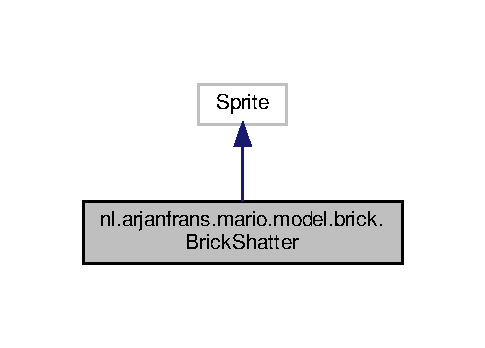
\includegraphics[width=233pt]{classnl_1_1arjanfrans_1_1mario_1_1model_1_1brick_1_1BrickShatter__inherit__graph}
\end{center}
\end{figure}


Collaboration diagram for nl.\+arjanfrans.\+mario.\+model.\+brick.\+Brick\+Shatter\+:
\nopagebreak
\begin{figure}[H]
\begin{center}
\leavevmode
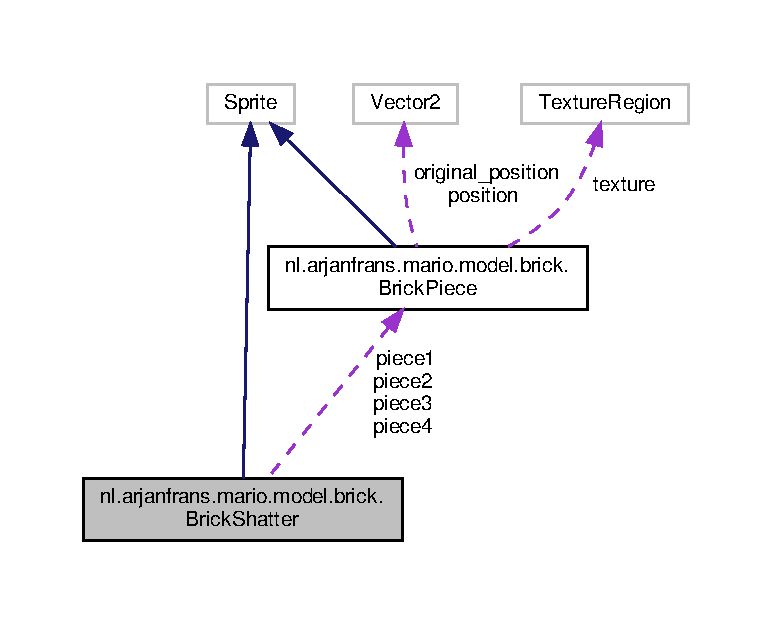
\includegraphics[width=350pt]{classnl_1_1arjanfrans_1_1mario_1_1model_1_1brick_1_1BrickShatter__coll__graph}
\end{center}
\end{figure}
\subsection*{Public Member Functions}
\begin{DoxyCompactItemize}
\item 
\hyperlink{classnl_1_1arjanfrans_1_1mario_1_1model_1_1brick_1_1BrickShatter_a5ea2c39e2ee5b639935f1a3102f2e4a9}{Brick\+Shatter} (float x, float y)
\begin{DoxyCompactList}\small\item\em Constructor method for \hyperlink{classnl_1_1arjanfrans_1_1mario_1_1model_1_1brick_1_1BrickShatter}{Brick\+Shatter}. \end{DoxyCompactList}\item 
void \hyperlink{classnl_1_1arjanfrans_1_1mario_1_1model_1_1brick_1_1BrickShatter_a905743105e75d0c38df647508d51ffa8}{draw} (Batch batch)
\begin{DoxyCompactList}\small\item\em This is the method meant to draw a \hyperlink{classnl_1_1arjanfrans_1_1mario_1_1model_1_1brick_1_1BrickShatter}{Brick\+Shatter}. \end{DoxyCompactList}\end{DoxyCompactItemize}
\subsection*{Private Attributes}
\begin{DoxyCompactItemize}
\item 
\mbox{\Hypertarget{classnl_1_1arjanfrans_1_1mario_1_1model_1_1brick_1_1BrickShatter_ad2e96eaadb09408cda11ad7fd99dd1bb}\label{classnl_1_1arjanfrans_1_1mario_1_1model_1_1brick_1_1BrickShatter_ad2e96eaadb09408cda11ad7fd99dd1bb}} 
\hyperlink{classnl_1_1arjanfrans_1_1mario_1_1model_1_1brick_1_1BrickPiece}{Brick\+Piece} {\bfseries piece1}
\item 
\mbox{\Hypertarget{classnl_1_1arjanfrans_1_1mario_1_1model_1_1brick_1_1BrickShatter_aade6a079b36b6d0891b7ad80a248551c}\label{classnl_1_1arjanfrans_1_1mario_1_1model_1_1brick_1_1BrickShatter_aade6a079b36b6d0891b7ad80a248551c}} 
\hyperlink{classnl_1_1arjanfrans_1_1mario_1_1model_1_1brick_1_1BrickPiece}{Brick\+Piece} {\bfseries piece2}
\item 
\mbox{\Hypertarget{classnl_1_1arjanfrans_1_1mario_1_1model_1_1brick_1_1BrickShatter_a554359af225e73feb086b62a4daf1a00}\label{classnl_1_1arjanfrans_1_1mario_1_1model_1_1brick_1_1BrickShatter_a554359af225e73feb086b62a4daf1a00}} 
\hyperlink{classnl_1_1arjanfrans_1_1mario_1_1model_1_1brick_1_1BrickPiece}{Brick\+Piece} {\bfseries piece3}
\item 
\mbox{\Hypertarget{classnl_1_1arjanfrans_1_1mario_1_1model_1_1brick_1_1BrickShatter_a9fc97e4bf031b32e1a941336e0bcd50e}\label{classnl_1_1arjanfrans_1_1mario_1_1model_1_1brick_1_1BrickShatter_a9fc97e4bf031b32e1a941336e0bcd50e}} 
\hyperlink{classnl_1_1arjanfrans_1_1mario_1_1model_1_1brick_1_1BrickPiece}{Brick\+Piece} {\bfseries piece4}
\end{DoxyCompactItemize}


\subsection{Detailed Description}
This class is the class meant to model the shattering of the bricks in the game. 

\subsection{Constructor \& Destructor Documentation}
\mbox{\Hypertarget{classnl_1_1arjanfrans_1_1mario_1_1model_1_1brick_1_1BrickShatter_a5ea2c39e2ee5b639935f1a3102f2e4a9}\label{classnl_1_1arjanfrans_1_1mario_1_1model_1_1brick_1_1BrickShatter_a5ea2c39e2ee5b639935f1a3102f2e4a9}} 
\index{nl\+::arjanfrans\+::mario\+::model\+::brick\+::\+Brick\+Shatter@{nl\+::arjanfrans\+::mario\+::model\+::brick\+::\+Brick\+Shatter}!Brick\+Shatter@{Brick\+Shatter}}
\index{Brick\+Shatter@{Brick\+Shatter}!nl\+::arjanfrans\+::mario\+::model\+::brick\+::\+Brick\+Shatter@{nl\+::arjanfrans\+::mario\+::model\+::brick\+::\+Brick\+Shatter}}
\subsubsection{\texorpdfstring{Brick\+Shatter()}{BrickShatter()}}
{\footnotesize\ttfamily nl.\+arjanfrans.\+mario.\+model.\+brick.\+Brick\+Shatter.\+Brick\+Shatter (\begin{DoxyParamCaption}\item[{float}]{x,  }\item[{float}]{y }\end{DoxyParamCaption})}



Constructor method for \hyperlink{classnl_1_1arjanfrans_1_1mario_1_1model_1_1brick_1_1BrickShatter}{Brick\+Shatter}. 


\begin{DoxyParams}{Parameters}
{\em x} & -\/ base x coordinate of the brick pieces \\
\hline
{\em y} & -\/ base y coordinate of the brick pieces \\
\hline
\end{DoxyParams}
\begin{DoxyReturn}{Returns}
an instance of \hyperlink{classnl_1_1arjanfrans_1_1mario_1_1model_1_1brick_1_1BrickShatter}{Brick\+Shatter} 
\end{DoxyReturn}


\subsection{Member Function Documentation}
\mbox{\Hypertarget{classnl_1_1arjanfrans_1_1mario_1_1model_1_1brick_1_1BrickShatter_a905743105e75d0c38df647508d51ffa8}\label{classnl_1_1arjanfrans_1_1mario_1_1model_1_1brick_1_1BrickShatter_a905743105e75d0c38df647508d51ffa8}} 
\index{nl\+::arjanfrans\+::mario\+::model\+::brick\+::\+Brick\+Shatter@{nl\+::arjanfrans\+::mario\+::model\+::brick\+::\+Brick\+Shatter}!draw@{draw}}
\index{draw@{draw}!nl\+::arjanfrans\+::mario\+::model\+::brick\+::\+Brick\+Shatter@{nl\+::arjanfrans\+::mario\+::model\+::brick\+::\+Brick\+Shatter}}
\subsubsection{\texorpdfstring{draw()}{draw()}}
{\footnotesize\ttfamily void nl.\+arjanfrans.\+mario.\+model.\+brick.\+Brick\+Shatter.\+draw (\begin{DoxyParamCaption}\item[{Batch}]{batch }\end{DoxyParamCaption})}



This is the method meant to draw a \hyperlink{classnl_1_1arjanfrans_1_1mario_1_1model_1_1brick_1_1BrickShatter}{Brick\+Shatter}. 


\begin{DoxyParams}{Parameters}
{\em batch} & -\/ an object used to draw 2D rectangles that reference a texture (region). \\
\hline
\end{DoxyParams}


The documentation for this class was generated from the following file\+:\begin{DoxyCompactItemize}
\item 
core/src/nl/arjanfrans/mario/model/brick/Brick\+Shatter.\+java\end{DoxyCompactItemize}

\hypertarget{classnl_1_1arjanfrans_1_1mario_1_1graphics_1_1CharacterAnimation}{}\section{nl.\+arjanfrans.\+mario.\+graphics.\+Character\+Animation Class Reference}
\label{classnl_1_1arjanfrans_1_1mario_1_1graphics_1_1CharacterAnimation}\index{nl.\+arjanfrans.\+mario.\+graphics.\+Character\+Animation@{nl.\+arjanfrans.\+mario.\+graphics.\+Character\+Animation}}


This is an abstract class that will be implemented to handle the animations of various characters in the game.  




Inheritance diagram for nl.\+arjanfrans.\+mario.\+graphics.\+Character\+Animation\+:
\nopagebreak
\begin{figure}[H]
\begin{center}
\leavevmode
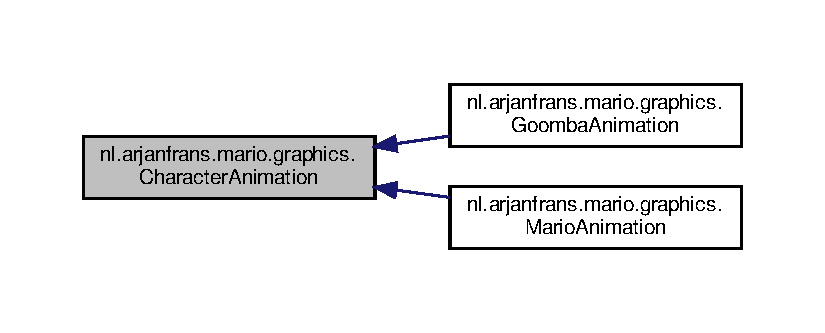
\includegraphics[width=350pt]{classnl_1_1arjanfrans_1_1mario_1_1graphics_1_1CharacterAnimation__inherit__graph}
\end{center}
\end{figure}


Collaboration diagram for nl.\+arjanfrans.\+mario.\+graphics.\+Character\+Animation\+:\nopagebreak
\begin{figure}[H]
\begin{center}
\leavevmode
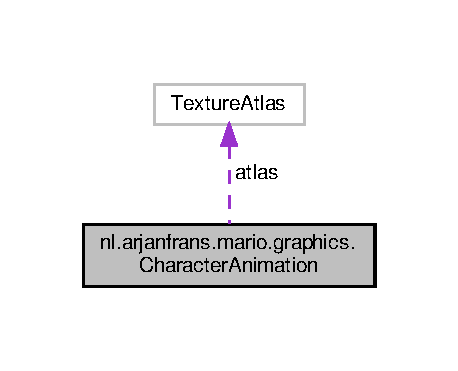
\includegraphics[width=220pt]{classnl_1_1arjanfrans_1_1mario_1_1graphics_1_1CharacterAnimation__coll__graph}
\end{center}
\end{figure}
\subsection*{Public Member Functions}
\begin{DoxyCompactItemize}
\item 
\mbox{\Hypertarget{classnl_1_1arjanfrans_1_1mario_1_1graphics_1_1CharacterAnimation_a880fedd9a315fa5f2ad2aa1e51b9f05e}\label{classnl_1_1arjanfrans_1_1mario_1_1graphics_1_1CharacterAnimation_a880fedd9a315fa5f2ad2aa1e51b9f05e}} 
void \hyperlink{classnl_1_1arjanfrans_1_1mario_1_1graphics_1_1CharacterAnimation_a880fedd9a315fa5f2ad2aa1e51b9f05e}{dispose} ()
\begin{DoxyCompactList}\small\item\em This method disposes of the animation. \end{DoxyCompactList}\end{DoxyCompactItemize}
\subsection*{Static Public Attributes}
\begin{DoxyCompactItemize}
\item 
\mbox{\Hypertarget{classnl_1_1arjanfrans_1_1mario_1_1graphics_1_1CharacterAnimation_a940a01ff1fb29a7a4814e2be10d78122}\label{classnl_1_1arjanfrans_1_1mario_1_1graphics_1_1CharacterAnimation_a940a01ff1fb29a7a4814e2be10d78122}} 
static final float {\bfseries scale} = 1/16f
\end{DoxyCompactItemize}
\subsection*{Protected Attributes}
\begin{DoxyCompactItemize}
\item 
\mbox{\Hypertarget{classnl_1_1arjanfrans_1_1mario_1_1graphics_1_1CharacterAnimation_a164e4424f77ef8d425d21e3f3553e5ca}\label{classnl_1_1arjanfrans_1_1mario_1_1graphics_1_1CharacterAnimation_a164e4424f77ef8d425d21e3f3553e5ca}} 
Texture\+Atlas {\bfseries atlas} = new Texture\+Atlas(\char`\"{}data/characters/characters.\+atlas\char`\"{})
\end{DoxyCompactItemize}


\subsection{Detailed Description}
This is an abstract class that will be implemented to handle the animations of various characters in the game. 

The documentation for this class was generated from the following file\+:\begin{DoxyCompactItemize}
\item 
core/src/nl/arjanfrans/mario/graphics/Character\+Animation.\+java\end{DoxyCompactItemize}

\hypertarget{classnl_1_1arjanfrans_1_1mario_1_1model_1_1Creature}{}\section{nl.\+arjanfrans.\+mario.\+model.\+Creature Class Reference}
\label{classnl_1_1arjanfrans_1_1mario_1_1model_1_1Creature}\index{nl.\+arjanfrans.\+mario.\+model.\+Creature@{nl.\+arjanfrans.\+mario.\+model.\+Creature}}


This class is the class model to represent any moving actor that is interactive, and not \hyperlink{classnl_1_1arjanfrans_1_1mario_1_1model_1_1Mario}{Mario}.  




Inheritance diagram for nl.\+arjanfrans.\+mario.\+model.\+Creature\+:
\nopagebreak
\begin{figure}[H]
\begin{center}
\leavevmode
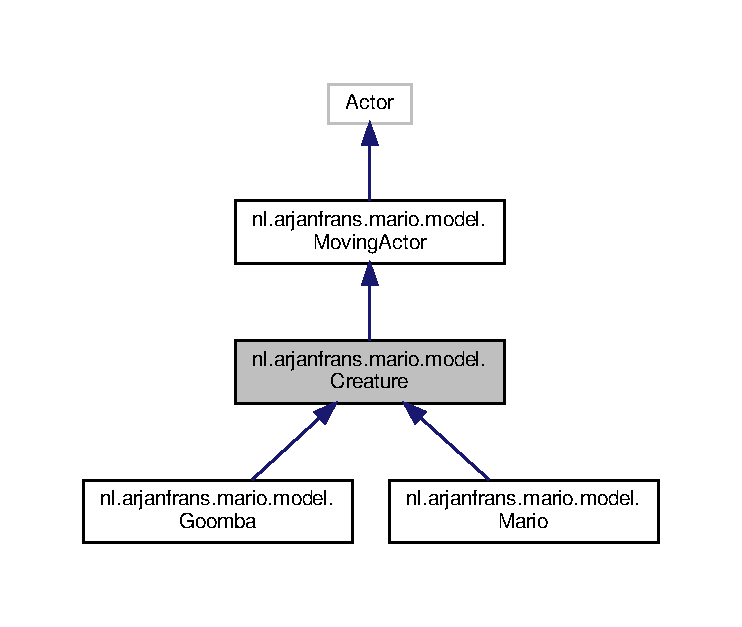
\includegraphics[width=350pt]{classnl_1_1arjanfrans_1_1mario_1_1model_1_1Creature__inherit__graph}
\end{center}
\end{figure}


Collaboration diagram for nl.\+arjanfrans.\+mario.\+model.\+Creature\+:
\nopagebreak
\begin{figure}[H]
\begin{center}
\leavevmode
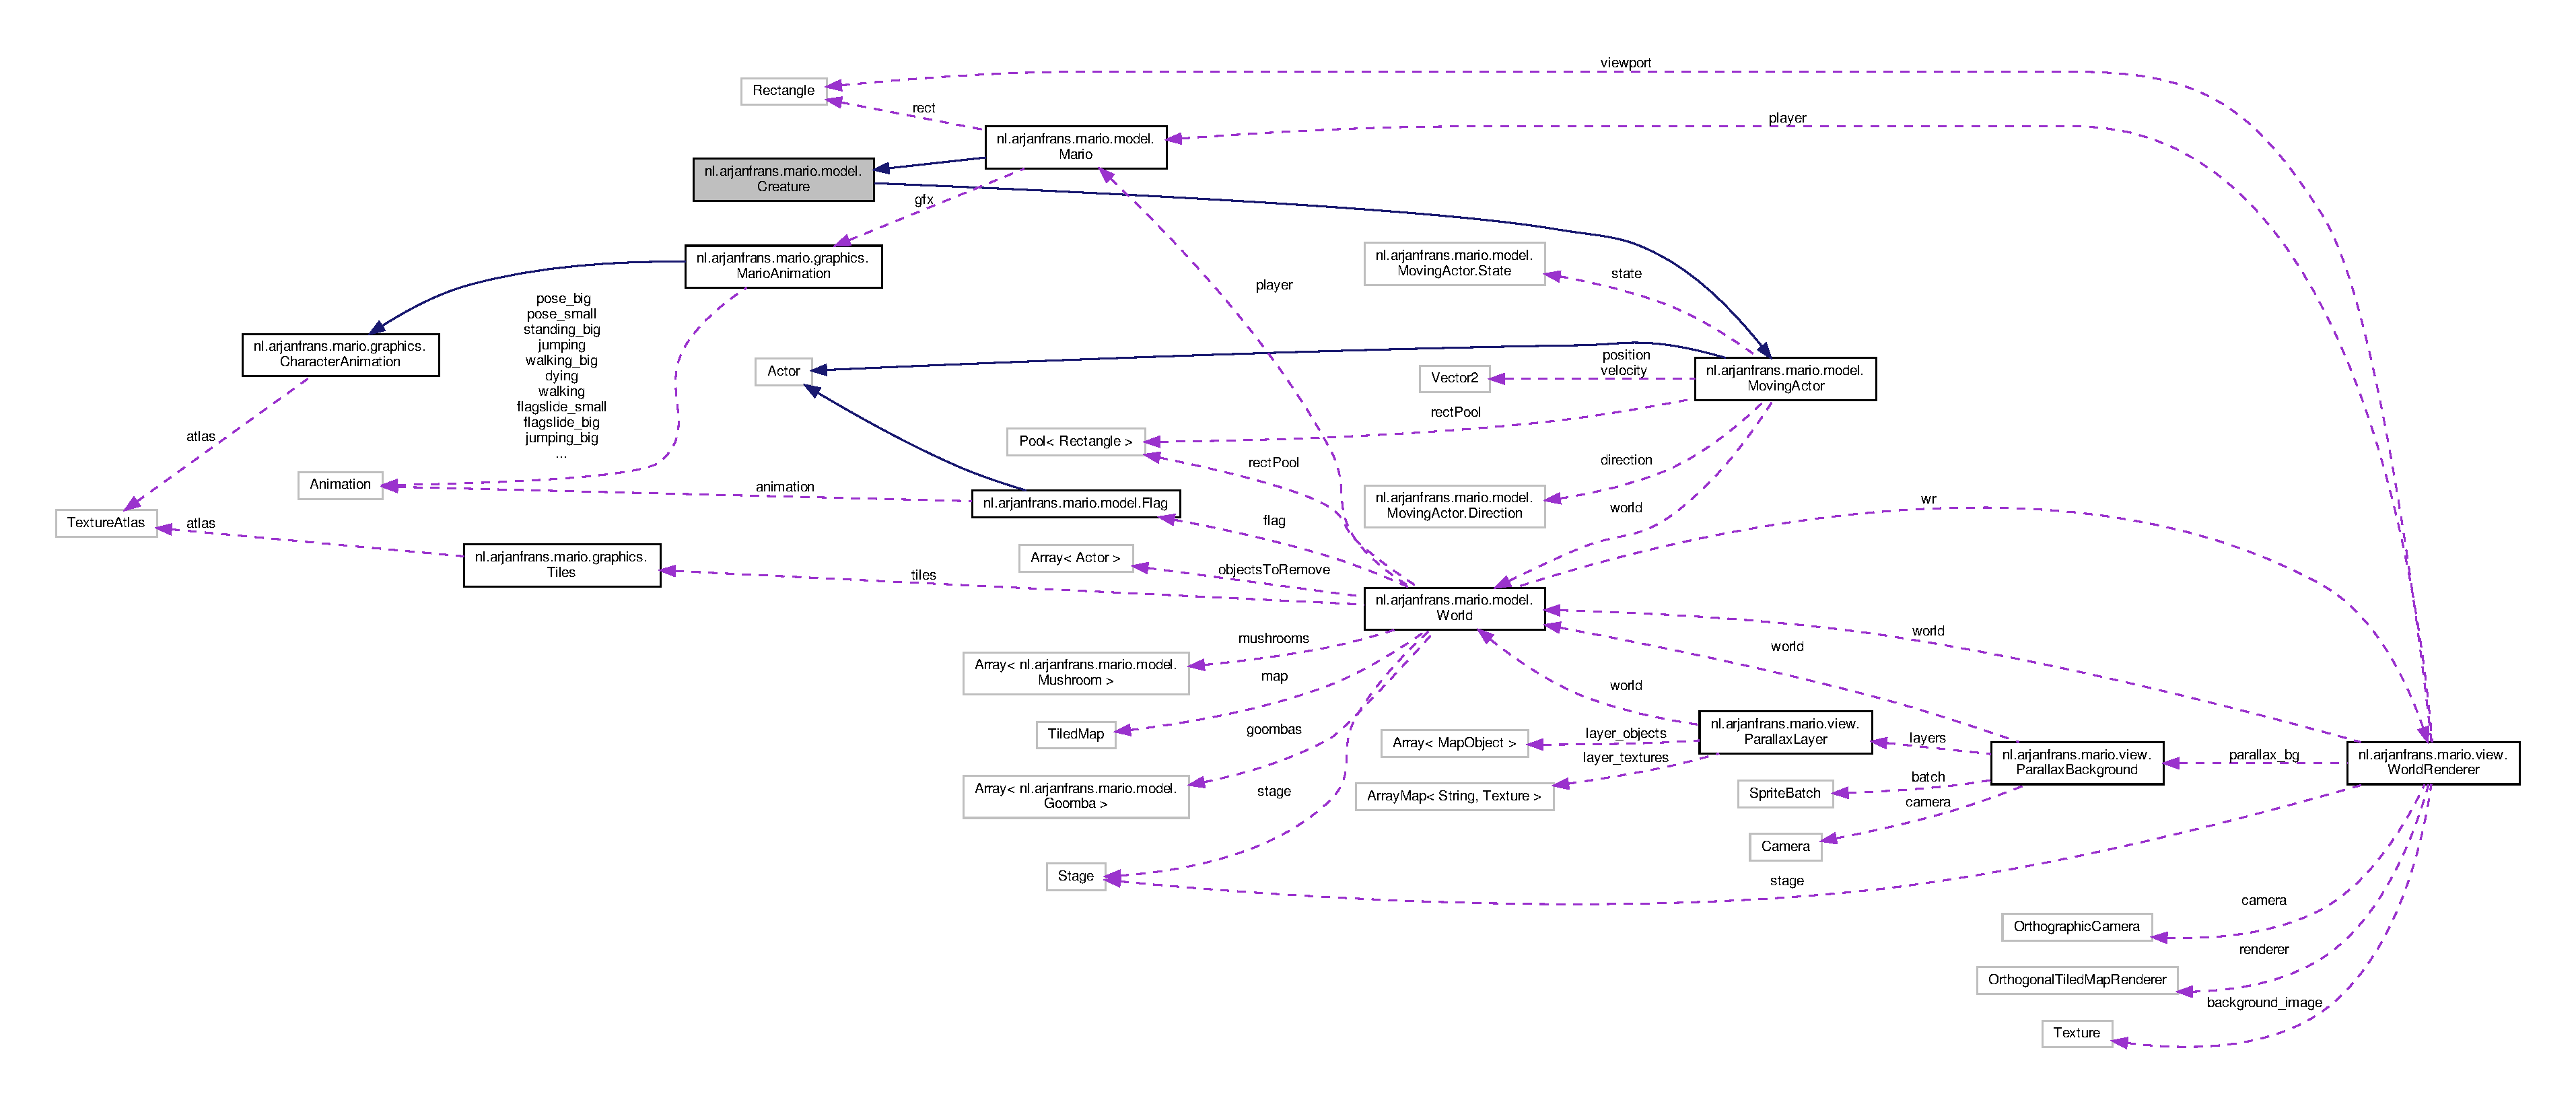
\includegraphics[width=350pt]{classnl_1_1arjanfrans_1_1mario_1_1model_1_1Creature__coll__graph}
\end{center}
\end{figure}
\subsection*{Public Member Functions}
\begin{DoxyCompactItemize}
\item 
\hyperlink{classnl_1_1arjanfrans_1_1mario_1_1model_1_1Creature_ab8c69d6a20f23355757ee4275a607086}{Creature} (\hyperlink{classnl_1_1arjanfrans_1_1mario_1_1model_1_1World}{World} world, float positionX, float positionY, float f)
\begin{DoxyCompactList}\small\item\em Constructor method. \end{DoxyCompactList}\item 
\mbox{\Hypertarget{classnl_1_1arjanfrans_1_1mario_1_1model_1_1Creature_af90d849667c2f64b1b578f27e575f444}\label{classnl_1_1arjanfrans_1_1mario_1_1model_1_1Creature_af90d849667c2f64b1b578f27e575f444}} 
abstract Animation \hyperlink{classnl_1_1arjanfrans_1_1mario_1_1model_1_1Creature_af90d849667c2f64b1b578f27e575f444}{get\+Animation} ()
\begin{DoxyCompactList}\small\item\em Gets the animation of the creature. \end{DoxyCompactList}\end{DoxyCompactItemize}
\subsection*{Protected Member Functions}
\begin{DoxyCompactItemize}
\item 
\mbox{\Hypertarget{classnl_1_1arjanfrans_1_1mario_1_1model_1_1Creature_acde9170546655c54aa46b98f35845845}\label{classnl_1_1arjanfrans_1_1mario_1_1model_1_1Creature_acde9170546655c54aa46b98f35845845}} 
abstract void \hyperlink{classnl_1_1arjanfrans_1_1mario_1_1model_1_1Creature_acde9170546655c54aa46b98f35845845}{die\+By\+Falling} ()
\begin{DoxyCompactList}\small\item\em Eliminates the creature when it dies by falling. \end{DoxyCompactList}\item 
\mbox{\Hypertarget{classnl_1_1arjanfrans_1_1mario_1_1model_1_1Creature_ac8a2e1db675c8efb0723e5750de80c41}\label{classnl_1_1arjanfrans_1_1mario_1_1model_1_1Creature_ac8a2e1db675c8efb0723e5750de80c41}} 
abstract void \hyperlink{classnl_1_1arjanfrans_1_1mario_1_1model_1_1Creature_ac8a2e1db675c8efb0723e5750de80c41}{collision\+X\+Action} ()
\begin{DoxyCompactList}\small\item\em Describes behaviour when creature interacts with object in the X direction. \end{DoxyCompactList}\end{DoxyCompactItemize}
\subsection*{Additional Inherited Members}


\subsection{Detailed Description}
This class is the class model to represent any moving actor that is interactive, and not \hyperlink{classnl_1_1arjanfrans_1_1mario_1_1model_1_1Mario}{Mario}. 

\subsection{Constructor \& Destructor Documentation}
\mbox{\Hypertarget{classnl_1_1arjanfrans_1_1mario_1_1model_1_1Creature_ab8c69d6a20f23355757ee4275a607086}\label{classnl_1_1arjanfrans_1_1mario_1_1model_1_1Creature_ab8c69d6a20f23355757ee4275a607086}} 
\index{nl\+::arjanfrans\+::mario\+::model\+::\+Creature@{nl\+::arjanfrans\+::mario\+::model\+::\+Creature}!Creature@{Creature}}
\index{Creature@{Creature}!nl\+::arjanfrans\+::mario\+::model\+::\+Creature@{nl\+::arjanfrans\+::mario\+::model\+::\+Creature}}
\subsubsection{\texorpdfstring{Creature()}{Creature()}}
{\footnotesize\ttfamily nl.\+arjanfrans.\+mario.\+model.\+Creature.\+Creature (\begin{DoxyParamCaption}\item[{\hyperlink{classnl_1_1arjanfrans_1_1mario_1_1model_1_1World}{World}}]{world,  }\item[{float}]{positionX,  }\item[{float}]{positionY,  }\item[{float}]{f }\end{DoxyParamCaption})}



Constructor method. 

Method which initializes and instance of \hyperlink{classnl_1_1arjanfrans_1_1mario_1_1model_1_1Creature}{Creature} 
\begin{DoxyParams}{Parameters}
{\em world} & \hyperlink{classnl_1_1arjanfrans_1_1mario_1_1model_1_1World}{World} object which defines which game instance the creature exists in \\
\hline
{\em positionX} & The initial x coordinate for the creature \\
\hline
{\em positionY} & The initial y coordinate for the creature \\
\hline
{\em f} & Height of the creature \\
\hline
\end{DoxyParams}
\begin{DoxyReturn}{Returns}
An instance of \hyperlink{classnl_1_1arjanfrans_1_1mario_1_1model_1_1Creature}{Creature} 
\end{DoxyReturn}


The documentation for this class was generated from the following file\+:\begin{DoxyCompactItemize}
\item 
core/src/nl/arjanfrans/mario/model/\hyperlink{Creature_8java}{Creature.\+java}\end{DoxyCompactItemize}

\hypertarget{classnl_1_1arjanfrans_1_1mario_1_1debug_1_1D}{}\section{nl.\+arjanfrans.\+mario.\+debug.\+D Class Reference}
\label{classnl_1_1arjanfrans_1_1mario_1_1debug_1_1D}\index{nl.\+arjanfrans.\+mario.\+debug.\+D@{nl.\+arjanfrans.\+mario.\+debug.\+D}}


Debug class.  


\subsection*{Static Public Member Functions}
\begin{DoxyCompactItemize}
\item 
static void \hyperlink{classnl_1_1arjanfrans_1_1mario_1_1debug_1_1D_a5b0a7c7830cdd12a95818ad5c114ed3c}{o} (String msg)
\begin{DoxyCompactList}\small\item\em Print debug message. \end{DoxyCompactList}\item 
static void \hyperlink{classnl_1_1arjanfrans_1_1mario_1_1debug_1_1D_aa2b3bc37c1340bc9978ab30a3970e26e}{o} (float msg)
\begin{DoxyCompactList}\small\item\em Print debug message. \end{DoxyCompactList}\end{DoxyCompactItemize}


\subsection{Detailed Description}
Debug class. 

\subsection{Member Function Documentation}
\mbox{\Hypertarget{classnl_1_1arjanfrans_1_1mario_1_1debug_1_1D_a5b0a7c7830cdd12a95818ad5c114ed3c}\label{classnl_1_1arjanfrans_1_1mario_1_1debug_1_1D_a5b0a7c7830cdd12a95818ad5c114ed3c}} 
\index{nl\+::arjanfrans\+::mario\+::debug\+::D@{nl\+::arjanfrans\+::mario\+::debug\+::D}!o@{o}}
\index{o@{o}!nl\+::arjanfrans\+::mario\+::debug\+::D@{nl\+::arjanfrans\+::mario\+::debug\+::D}}
\subsubsection{\texorpdfstring{o()}{o()}\hspace{0.1cm}{\footnotesize\ttfamily [1/2]}}
{\footnotesize\ttfamily static void nl.\+arjanfrans.\+mario.\+debug.\+D.\+o (\begin{DoxyParamCaption}\item[{String}]{msg }\end{DoxyParamCaption})\hspace{0.3cm}{\ttfamily [static]}}



Print debug message. 


\begin{DoxyParams}{Parameters}
{\em msg} & String value \\
\hline
\end{DoxyParams}
\mbox{\Hypertarget{classnl_1_1arjanfrans_1_1mario_1_1debug_1_1D_aa2b3bc37c1340bc9978ab30a3970e26e}\label{classnl_1_1arjanfrans_1_1mario_1_1debug_1_1D_aa2b3bc37c1340bc9978ab30a3970e26e}} 
\index{nl\+::arjanfrans\+::mario\+::debug\+::D@{nl\+::arjanfrans\+::mario\+::debug\+::D}!o@{o}}
\index{o@{o}!nl\+::arjanfrans\+::mario\+::debug\+::D@{nl\+::arjanfrans\+::mario\+::debug\+::D}}
\subsubsection{\texorpdfstring{o()}{o()}\hspace{0.1cm}{\footnotesize\ttfamily [2/2]}}
{\footnotesize\ttfamily static void nl.\+arjanfrans.\+mario.\+debug.\+D.\+o (\begin{DoxyParamCaption}\item[{float}]{msg }\end{DoxyParamCaption})\hspace{0.3cm}{\ttfamily [static]}}



Print debug message. 


\begin{DoxyParams}{Parameters}
{\em msg} & float value \\
\hline
\end{DoxyParams}


The documentation for this class was generated from the following file\+:\begin{DoxyCompactItemize}
\item 
core/src/nl/arjanfrans/mario/debug/\hyperlink{D_8java}{D.\+java}\end{DoxyCompactItemize}

\hypertarget{classnl_1_1arjanfrans_1_1mario_1_1desktop_1_1DesktopLauncher}{}\section{nl.\+arjanfrans.\+mario.\+desktop.\+Desktop\+Launcher Class Reference}
\label{classnl_1_1arjanfrans_1_1mario_1_1desktop_1_1DesktopLauncher}\index{nl.\+arjanfrans.\+mario.\+desktop.\+Desktop\+Launcher@{nl.\+arjanfrans.\+mario.\+desktop.\+Desktop\+Launcher}}


This class is the main method allowing the game to initialize and launch.  


\subsection*{Static Public Member Functions}
\begin{DoxyCompactItemize}
\item 
static void \hyperlink{classnl_1_1arjanfrans_1_1mario_1_1desktop_1_1DesktopLauncher_a428f564507af2ce16685de5532f8ad0b}{main} (String\mbox{[}$\,$\mbox{]} arg)
\begin{DoxyCompactList}\small\item\em Main method. \end{DoxyCompactList}\end{DoxyCompactItemize}


\subsection{Detailed Description}
This class is the main method allowing the game to initialize and launch. 

\subsection{Member Function Documentation}
\mbox{\Hypertarget{classnl_1_1arjanfrans_1_1mario_1_1desktop_1_1DesktopLauncher_a428f564507af2ce16685de5532f8ad0b}\label{classnl_1_1arjanfrans_1_1mario_1_1desktop_1_1DesktopLauncher_a428f564507af2ce16685de5532f8ad0b}} 
\index{nl\+::arjanfrans\+::mario\+::desktop\+::\+Desktop\+Launcher@{nl\+::arjanfrans\+::mario\+::desktop\+::\+Desktop\+Launcher}!main@{main}}
\index{main@{main}!nl\+::arjanfrans\+::mario\+::desktop\+::\+Desktop\+Launcher@{nl\+::arjanfrans\+::mario\+::desktop\+::\+Desktop\+Launcher}}
\subsubsection{\texorpdfstring{main()}{main()}}
{\footnotesize\ttfamily static void nl.\+arjanfrans.\+mario.\+desktop.\+Desktop\+Launcher.\+main (\begin{DoxyParamCaption}\item[{String \mbox{[}$\,$\mbox{]}}]{arg }\end{DoxyParamCaption})\hspace{0.3cm}{\ttfamily [static]}}



Main method. 

Method which is launched to trigger the initialization of the game through lib\+G\+DX 
\begin{DoxyParams}{Parameters}
{\em arg} & -\/ an array of string arguments from the command line \\
\hline
\end{DoxyParams}


The documentation for this class was generated from the following file\+:\begin{DoxyCompactItemize}
\item 
desktop/src/nl/arjanfrans/mario/desktop/\hyperlink{DesktopLauncher_8java}{Desktop\+Launcher.\+java}\end{DoxyCompactItemize}

\hypertarget{classnl_1_1arjanfrans_1_1mario_1_1model_1_1Flag}{}\section{nl.\+arjanfrans.\+mario.\+model.\+Flag Class Reference}
\label{classnl_1_1arjanfrans_1_1mario_1_1model_1_1Flag}\index{nl.\+arjanfrans.\+mario.\+model.\+Flag@{nl.\+arjanfrans.\+mario.\+model.\+Flag}}


This flag represents the flag pole at the end of the stage that completes if \hyperlink{classnl_1_1arjanfrans_1_1mario_1_1model_1_1Mario}{Mario} interacts with it.  




Inheritance diagram for nl.\+arjanfrans.\+mario.\+model.\+Flag\+:\nopagebreak
\begin{figure}[H]
\begin{center}
\leavevmode
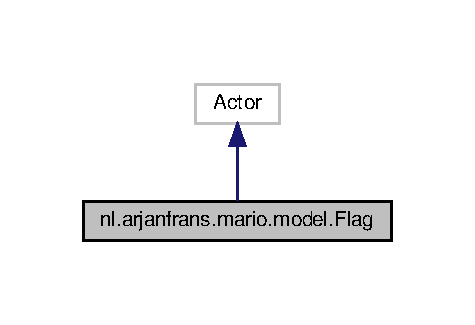
\includegraphics[width=228pt]{classnl_1_1arjanfrans_1_1mario_1_1model_1_1Flag__inherit__graph}
\end{center}
\end{figure}


Collaboration diagram for nl.\+arjanfrans.\+mario.\+model.\+Flag\+:\nopagebreak
\begin{figure}[H]
\begin{center}
\leavevmode
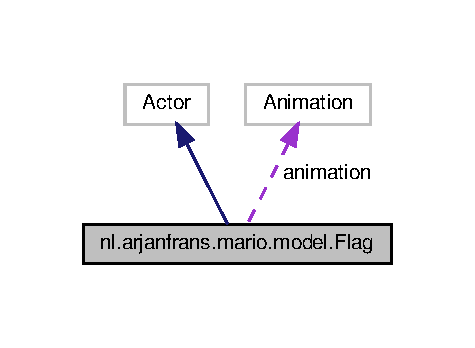
\includegraphics[width=228pt]{classnl_1_1arjanfrans_1_1mario_1_1model_1_1Flag__coll__graph}
\end{center}
\end{figure}
\subsection*{Public Member Functions}
\begin{DoxyCompactItemize}
\item 
\hyperlink{classnl_1_1arjanfrans_1_1mario_1_1model_1_1Flag_a69dcd8fbda6358ef4d2f0afbc273ef19}{Flag} (float x, float y, float width, float height, float \hyperlink{classnl_1_1arjanfrans_1_1mario_1_1model_1_1Flag_a3bbb2687c3bac27f6cee8ae891eddc16}{endX}, float \hyperlink{classnl_1_1arjanfrans_1_1mario_1_1model_1_1Flag_af5798cd4d07551f52e4b06e1b42efc19}{endY})
\begin{DoxyCompactList}\small\item\em Constructor method. \end{DoxyCompactList}\item 
void \hyperlink{classnl_1_1arjanfrans_1_1mario_1_1model_1_1Flag_a92c1d0b95a46934e2f9b286ca233452a}{act} (float delta)
\begin{DoxyCompactList}\small\item\em How the \hyperlink{classnl_1_1arjanfrans_1_1mario_1_1model_1_1Flag}{Flag} acts each time instance. \end{DoxyCompactList}\item 
void \hyperlink{classnl_1_1arjanfrans_1_1mario_1_1model_1_1Flag_accca18a710db846a8479e60be7fcc847}{take\+Down} ()
\begin{DoxyCompactList}\small\item\em \hyperlink{classnl_1_1arjanfrans_1_1mario_1_1model_1_1Mario}{Mario} captures flag. \end{DoxyCompactList}\item 
void \hyperlink{classnl_1_1arjanfrans_1_1mario_1_1model_1_1Flag_a37b444b2cce56fc741f29b12cfb9ebd0}{draw} (Batch batch, float parent\+Alpha)
\begin{DoxyCompactList}\small\item\em Draws the flag. \end{DoxyCompactList}\item 
Rectangle \hyperlink{classnl_1_1arjanfrans_1_1mario_1_1model_1_1Flag_a1602244ce7c750bd95ac7265e50ad557}{rect} ()
\begin{DoxyCompactList}\small\item\em Rectangle object in which the \hyperlink{classnl_1_1arjanfrans_1_1mario_1_1model_1_1Flag}{Flag} exists in. \end{DoxyCompactList}\item 
float \hyperlink{classnl_1_1arjanfrans_1_1mario_1_1model_1_1Flag_ae6e50aebb2bedd7b306ee99685212b2c}{get\+EndX} ()
\begin{DoxyCompactList}\small\item\em Gets end X coordinate. \end{DoxyCompactList}\item 
float \hyperlink{classnl_1_1arjanfrans_1_1mario_1_1model_1_1Flag_a0dee35b76827d958f8054e2fb5854a7b}{get\+EndY} ()
\begin{DoxyCompactList}\small\item\em Gets end Y coordinate. \end{DoxyCompactList}\item 
boolean \hyperlink{classnl_1_1arjanfrans_1_1mario_1_1model_1_1Flag_aee023da973eca87f5ba2c809d81d4379}{is\+Down} ()
\begin{DoxyCompactList}\small\item\em Gets whether the flag is down or not. \end{DoxyCompactList}\item 
void \hyperlink{classnl_1_1arjanfrans_1_1mario_1_1model_1_1Flag_a782bc6aff5cbac7ae16c17e31f2d8887}{set\+Down} (boolean \hyperlink{classnl_1_1arjanfrans_1_1mario_1_1model_1_1Flag_a60f19c488013d7598681a199cd60f109}{down})
\begin{DoxyCompactList}\small\item\em Sets the flag to the down state. \end{DoxyCompactList}\end{DoxyCompactItemize}
\subsection*{Private Attributes}
\begin{DoxyCompactItemize}
\item 
Animation \hyperlink{classnl_1_1arjanfrans_1_1mario_1_1model_1_1Flag_a0ae6225f7cd85bb4258325be58a92a5b}{animation}
\item 
float \hyperlink{classnl_1_1arjanfrans_1_1mario_1_1model_1_1Flag_adef15ac263403cee29a647f402a49167}{state\+Time}
\item 
float \hyperlink{classnl_1_1arjanfrans_1_1mario_1_1model_1_1Flag_a3bbb2687c3bac27f6cee8ae891eddc16}{endX}
\item 
float \hyperlink{classnl_1_1arjanfrans_1_1mario_1_1model_1_1Flag_af5798cd4d07551f52e4b06e1b42efc19}{endY}
\item 
boolean \hyperlink{classnl_1_1arjanfrans_1_1mario_1_1model_1_1Flag_a60f19c488013d7598681a199cd60f109}{down} = false
\item 
float \hyperlink{classnl_1_1arjanfrans_1_1mario_1_1model_1_1Flag_a9bd441f257959ac2fc23e18675a80db2}{bottomY}
\item 
float \hyperlink{classnl_1_1arjanfrans_1_1mario_1_1model_1_1Flag_ac3544e1ccdb436d5b980426f7a7a0f4c}{slide\+Offset} = 2
\end{DoxyCompactItemize}


\subsection{Detailed Description}
This flag represents the flag pole at the end of the stage that completes if \hyperlink{classnl_1_1arjanfrans_1_1mario_1_1model_1_1Mario}{Mario} interacts with it. 

\subsection{Constructor \& Destructor Documentation}
\mbox{\Hypertarget{classnl_1_1arjanfrans_1_1mario_1_1model_1_1Flag_a69dcd8fbda6358ef4d2f0afbc273ef19}\label{classnl_1_1arjanfrans_1_1mario_1_1model_1_1Flag_a69dcd8fbda6358ef4d2f0afbc273ef19}} 
\index{nl\+::arjanfrans\+::mario\+::model\+::\+Flag@{nl\+::arjanfrans\+::mario\+::model\+::\+Flag}!Flag@{Flag}}
\index{Flag@{Flag}!nl\+::arjanfrans\+::mario\+::model\+::\+Flag@{nl\+::arjanfrans\+::mario\+::model\+::\+Flag}}
\subsubsection{\texorpdfstring{Flag()}{Flag()}}
{\footnotesize\ttfamily nl.\+arjanfrans.\+mario.\+model.\+Flag.\+Flag (\begin{DoxyParamCaption}\item[{float}]{x,  }\item[{float}]{y,  }\item[{float}]{width,  }\item[{float}]{height,  }\item[{float}]{endX,  }\item[{float}]{endY }\end{DoxyParamCaption})}



Constructor method. 

Method which initializes an instance of \hyperlink{classnl_1_1arjanfrans_1_1mario_1_1model_1_1Flag}{Flag} 
\begin{DoxyParams}{Parameters}
{\em x} & x coordinate of the position of the \hyperlink{classnl_1_1arjanfrans_1_1mario_1_1model_1_1Flag}{Flag} \\
\hline
{\em y} & y coordinate of the position of the \hyperlink{classnl_1_1arjanfrans_1_1mario_1_1model_1_1Flag}{Flag} \\
\hline
{\em width} & The width of the \hyperlink{classnl_1_1arjanfrans_1_1mario_1_1model_1_1Flag}{Flag} \\
\hline
{\em height} & The height of the \hyperlink{classnl_1_1arjanfrans_1_1mario_1_1model_1_1Flag}{Flag} \\
\hline
{\em endX} & x coordinate to describe where the \hyperlink{classnl_1_1arjanfrans_1_1mario_1_1model_1_1Flag}{Flag} ends \\
\hline
{\em endY} & y coordinate to describe where the \hyperlink{classnl_1_1arjanfrans_1_1mario_1_1model_1_1Flag}{Flag} ends \\
\hline
\end{DoxyParams}
\begin{DoxyReturn}{Returns}
An instance of \hyperlink{classnl_1_1arjanfrans_1_1mario_1_1model_1_1Flag}{Flag} 
\end{DoxyReturn}


\subsection{Member Function Documentation}
\mbox{\Hypertarget{classnl_1_1arjanfrans_1_1mario_1_1model_1_1Flag_a92c1d0b95a46934e2f9b286ca233452a}\label{classnl_1_1arjanfrans_1_1mario_1_1model_1_1Flag_a92c1d0b95a46934e2f9b286ca233452a}} 
\index{nl\+::arjanfrans\+::mario\+::model\+::\+Flag@{nl\+::arjanfrans\+::mario\+::model\+::\+Flag}!act@{act}}
\index{act@{act}!nl\+::arjanfrans\+::mario\+::model\+::\+Flag@{nl\+::arjanfrans\+::mario\+::model\+::\+Flag}}
\subsubsection{\texorpdfstring{act()}{act()}}
{\footnotesize\ttfamily void nl.\+arjanfrans.\+mario.\+model.\+Flag.\+act (\begin{DoxyParamCaption}\item[{float}]{delta }\end{DoxyParamCaption})}



How the \hyperlink{classnl_1_1arjanfrans_1_1mario_1_1model_1_1Flag}{Flag} acts each time instance. 

After each discrete time step, this method is called and the state time is updated 
\begin{DoxyParams}{Parameters}
{\em delta} & The change in time for the actor \\
\hline
\end{DoxyParams}
\mbox{\Hypertarget{classnl_1_1arjanfrans_1_1mario_1_1model_1_1Flag_a37b444b2cce56fc741f29b12cfb9ebd0}\label{classnl_1_1arjanfrans_1_1mario_1_1model_1_1Flag_a37b444b2cce56fc741f29b12cfb9ebd0}} 
\index{nl\+::arjanfrans\+::mario\+::model\+::\+Flag@{nl\+::arjanfrans\+::mario\+::model\+::\+Flag}!draw@{draw}}
\index{draw@{draw}!nl\+::arjanfrans\+::mario\+::model\+::\+Flag@{nl\+::arjanfrans\+::mario\+::model\+::\+Flag}}
\subsubsection{\texorpdfstring{draw()}{draw()}}
{\footnotesize\ttfamily void nl.\+arjanfrans.\+mario.\+model.\+Flag.\+draw (\begin{DoxyParamCaption}\item[{Batch}]{batch,  }\item[{float}]{parent\+Alpha }\end{DoxyParamCaption})}



Draws the flag. 

Assists lib\+G\+DX in drawing the \hyperlink{classnl_1_1arjanfrans_1_1mario_1_1model_1_1Flag}{Flag} into the world, defines position and animation 
\begin{DoxyParams}{Parameters}
{\em batch} & Texture region where the \hyperlink{classnl_1_1arjanfrans_1_1mario_1_1model_1_1Flag}{Flag} is being drawn \\
\hline
{\em parent\+Alpha} & Not used \\
\hline
\end{DoxyParams}
\mbox{\Hypertarget{classnl_1_1arjanfrans_1_1mario_1_1model_1_1Flag_ae6e50aebb2bedd7b306ee99685212b2c}\label{classnl_1_1arjanfrans_1_1mario_1_1model_1_1Flag_ae6e50aebb2bedd7b306ee99685212b2c}} 
\index{nl\+::arjanfrans\+::mario\+::model\+::\+Flag@{nl\+::arjanfrans\+::mario\+::model\+::\+Flag}!get\+EndX@{get\+EndX}}
\index{get\+EndX@{get\+EndX}!nl\+::arjanfrans\+::mario\+::model\+::\+Flag@{nl\+::arjanfrans\+::mario\+::model\+::\+Flag}}
\subsubsection{\texorpdfstring{get\+End\+X()}{getEndX()}}
{\footnotesize\ttfamily float nl.\+arjanfrans.\+mario.\+model.\+Flag.\+get\+EndX (\begin{DoxyParamCaption}{ }\end{DoxyParamCaption})}



Gets end X coordinate. 

\begin{DoxyReturn}{Returns}
Returns float representing the x coordinate where the rectangle surrounding the \hyperlink{classnl_1_1arjanfrans_1_1mario_1_1model_1_1Flag}{Flag} ends 
\end{DoxyReturn}
\mbox{\Hypertarget{classnl_1_1arjanfrans_1_1mario_1_1model_1_1Flag_a0dee35b76827d958f8054e2fb5854a7b}\label{classnl_1_1arjanfrans_1_1mario_1_1model_1_1Flag_a0dee35b76827d958f8054e2fb5854a7b}} 
\index{nl\+::arjanfrans\+::mario\+::model\+::\+Flag@{nl\+::arjanfrans\+::mario\+::model\+::\+Flag}!get\+EndY@{get\+EndY}}
\index{get\+EndY@{get\+EndY}!nl\+::arjanfrans\+::mario\+::model\+::\+Flag@{nl\+::arjanfrans\+::mario\+::model\+::\+Flag}}
\subsubsection{\texorpdfstring{get\+End\+Y()}{getEndY()}}
{\footnotesize\ttfamily float nl.\+arjanfrans.\+mario.\+model.\+Flag.\+get\+EndY (\begin{DoxyParamCaption}{ }\end{DoxyParamCaption})}



Gets end Y coordinate. 

\begin{DoxyReturn}{Returns}
Returns float representing the y coordinate where the rectangle surrounding the \hyperlink{classnl_1_1arjanfrans_1_1mario_1_1model_1_1Flag}{Flag} ends 
\end{DoxyReturn}
\mbox{\Hypertarget{classnl_1_1arjanfrans_1_1mario_1_1model_1_1Flag_aee023da973eca87f5ba2c809d81d4379}\label{classnl_1_1arjanfrans_1_1mario_1_1model_1_1Flag_aee023da973eca87f5ba2c809d81d4379}} 
\index{nl\+::arjanfrans\+::mario\+::model\+::\+Flag@{nl\+::arjanfrans\+::mario\+::model\+::\+Flag}!is\+Down@{is\+Down}}
\index{is\+Down@{is\+Down}!nl\+::arjanfrans\+::mario\+::model\+::\+Flag@{nl\+::arjanfrans\+::mario\+::model\+::\+Flag}}
\subsubsection{\texorpdfstring{is\+Down()}{isDown()}}
{\footnotesize\ttfamily boolean nl.\+arjanfrans.\+mario.\+model.\+Flag.\+is\+Down (\begin{DoxyParamCaption}{ }\end{DoxyParamCaption})}



Gets whether the flag is down or not. 

\begin{DoxyReturn}{Returns}
Returns boolean of whether the flag has been captured or not 
\end{DoxyReturn}
\mbox{\Hypertarget{classnl_1_1arjanfrans_1_1mario_1_1model_1_1Flag_a1602244ce7c750bd95ac7265e50ad557}\label{classnl_1_1arjanfrans_1_1mario_1_1model_1_1Flag_a1602244ce7c750bd95ac7265e50ad557}} 
\index{nl\+::arjanfrans\+::mario\+::model\+::\+Flag@{nl\+::arjanfrans\+::mario\+::model\+::\+Flag}!rect@{rect}}
\index{rect@{rect}!nl\+::arjanfrans\+::mario\+::model\+::\+Flag@{nl\+::arjanfrans\+::mario\+::model\+::\+Flag}}
\subsubsection{\texorpdfstring{rect()}{rect()}}
{\footnotesize\ttfamily Rectangle nl.\+arjanfrans.\+mario.\+model.\+Flag.\+rect (\begin{DoxyParamCaption}{ }\end{DoxyParamCaption})}



Rectangle object in which the \hyperlink{classnl_1_1arjanfrans_1_1mario_1_1model_1_1Flag}{Flag} exists in. 

\begin{DoxyReturn}{Returns}
Returns lib\+G\+DX rectangle object with this objects coordinates 
\end{DoxyReturn}
\mbox{\Hypertarget{classnl_1_1arjanfrans_1_1mario_1_1model_1_1Flag_a782bc6aff5cbac7ae16c17e31f2d8887}\label{classnl_1_1arjanfrans_1_1mario_1_1model_1_1Flag_a782bc6aff5cbac7ae16c17e31f2d8887}} 
\index{nl\+::arjanfrans\+::mario\+::model\+::\+Flag@{nl\+::arjanfrans\+::mario\+::model\+::\+Flag}!set\+Down@{set\+Down}}
\index{set\+Down@{set\+Down}!nl\+::arjanfrans\+::mario\+::model\+::\+Flag@{nl\+::arjanfrans\+::mario\+::model\+::\+Flag}}
\subsubsection{\texorpdfstring{set\+Down()}{setDown()}}
{\footnotesize\ttfamily void nl.\+arjanfrans.\+mario.\+model.\+Flag.\+set\+Down (\begin{DoxyParamCaption}\item[{boolean}]{down }\end{DoxyParamCaption})}



Sets the flag to the down state. 


\begin{DoxyParams}{Parameters}
{\em down} & A boolean representing whether the \hyperlink{classnl_1_1arjanfrans_1_1mario_1_1model_1_1Flag}{Flag} is in the down state or not \\
\hline
\end{DoxyParams}
\mbox{\Hypertarget{classnl_1_1arjanfrans_1_1mario_1_1model_1_1Flag_accca18a710db846a8479e60be7fcc847}\label{classnl_1_1arjanfrans_1_1mario_1_1model_1_1Flag_accca18a710db846a8479e60be7fcc847}} 
\index{nl\+::arjanfrans\+::mario\+::model\+::\+Flag@{nl\+::arjanfrans\+::mario\+::model\+::\+Flag}!take\+Down@{take\+Down}}
\index{take\+Down@{take\+Down}!nl\+::arjanfrans\+::mario\+::model\+::\+Flag@{nl\+::arjanfrans\+::mario\+::model\+::\+Flag}}
\subsubsection{\texorpdfstring{take\+Down()}{takeDown()}}
{\footnotesize\ttfamily void nl.\+arjanfrans.\+mario.\+model.\+Flag.\+take\+Down (\begin{DoxyParamCaption}{ }\end{DoxyParamCaption})}



\hyperlink{classnl_1_1arjanfrans_1_1mario_1_1model_1_1Mario}{Mario} captures flag. 

Triggered when \hyperlink{classnl_1_1arjanfrans_1_1mario_1_1model_1_1Mario}{Mario} interacts with the \hyperlink{classnl_1_1arjanfrans_1_1mario_1_1model_1_1Flag}{Flag} pole 

\subsection{Member Data Documentation}
\mbox{\Hypertarget{classnl_1_1arjanfrans_1_1mario_1_1model_1_1Flag_a0ae6225f7cd85bb4258325be58a92a5b}\label{classnl_1_1arjanfrans_1_1mario_1_1model_1_1Flag_a0ae6225f7cd85bb4258325be58a92a5b}} 
\index{nl\+::arjanfrans\+::mario\+::model\+::\+Flag@{nl\+::arjanfrans\+::mario\+::model\+::\+Flag}!animation@{animation}}
\index{animation@{animation}!nl\+::arjanfrans\+::mario\+::model\+::\+Flag@{nl\+::arjanfrans\+::mario\+::model\+::\+Flag}}
\subsubsection{\texorpdfstring{animation}{animation}}
{\footnotesize\ttfamily Animation nl.\+arjanfrans.\+mario.\+model.\+Flag.\+animation\hspace{0.3cm}{\ttfamily [private]}}

Animation that the flag displays \mbox{\Hypertarget{classnl_1_1arjanfrans_1_1mario_1_1model_1_1Flag_a9bd441f257959ac2fc23e18675a80db2}\label{classnl_1_1arjanfrans_1_1mario_1_1model_1_1Flag_a9bd441f257959ac2fc23e18675a80db2}} 
\index{nl\+::arjanfrans\+::mario\+::model\+::\+Flag@{nl\+::arjanfrans\+::mario\+::model\+::\+Flag}!bottomY@{bottomY}}
\index{bottomY@{bottomY}!nl\+::arjanfrans\+::mario\+::model\+::\+Flag@{nl\+::arjanfrans\+::mario\+::model\+::\+Flag}}
\subsubsection{\texorpdfstring{bottomY}{bottomY}}
{\footnotesize\ttfamily float nl.\+arjanfrans.\+mario.\+model.\+Flag.\+bottomY\hspace{0.3cm}{\ttfamily [private]}}

Y coordinate to describe the bottom of the flag \mbox{\Hypertarget{classnl_1_1arjanfrans_1_1mario_1_1model_1_1Flag_a60f19c488013d7598681a199cd60f109}\label{classnl_1_1arjanfrans_1_1mario_1_1model_1_1Flag_a60f19c488013d7598681a199cd60f109}} 
\index{nl\+::arjanfrans\+::mario\+::model\+::\+Flag@{nl\+::arjanfrans\+::mario\+::model\+::\+Flag}!down@{down}}
\index{down@{down}!nl\+::arjanfrans\+::mario\+::model\+::\+Flag@{nl\+::arjanfrans\+::mario\+::model\+::\+Flag}}
\subsubsection{\texorpdfstring{down}{down}}
{\footnotesize\ttfamily boolean nl.\+arjanfrans.\+mario.\+model.\+Flag.\+down = false\hspace{0.3cm}{\ttfamily [private]}}

If the flag has been captured or not \mbox{\Hypertarget{classnl_1_1arjanfrans_1_1mario_1_1model_1_1Flag_a3bbb2687c3bac27f6cee8ae891eddc16}\label{classnl_1_1arjanfrans_1_1mario_1_1model_1_1Flag_a3bbb2687c3bac27f6cee8ae891eddc16}} 
\index{nl\+::arjanfrans\+::mario\+::model\+::\+Flag@{nl\+::arjanfrans\+::mario\+::model\+::\+Flag}!endX@{endX}}
\index{endX@{endX}!nl\+::arjanfrans\+::mario\+::model\+::\+Flag@{nl\+::arjanfrans\+::mario\+::model\+::\+Flag}}
\subsubsection{\texorpdfstring{endX}{endX}}
{\footnotesize\ttfamily float nl.\+arjanfrans.\+mario.\+model.\+Flag.\+endX\hspace{0.3cm}{\ttfamily [private]}}

X coordinate to describe where the \hyperlink{classnl_1_1arjanfrans_1_1mario_1_1model_1_1Flag}{Flag} ends \mbox{\Hypertarget{classnl_1_1arjanfrans_1_1mario_1_1model_1_1Flag_af5798cd4d07551f52e4b06e1b42efc19}\label{classnl_1_1arjanfrans_1_1mario_1_1model_1_1Flag_af5798cd4d07551f52e4b06e1b42efc19}} 
\index{nl\+::arjanfrans\+::mario\+::model\+::\+Flag@{nl\+::arjanfrans\+::mario\+::model\+::\+Flag}!endY@{endY}}
\index{endY@{endY}!nl\+::arjanfrans\+::mario\+::model\+::\+Flag@{nl\+::arjanfrans\+::mario\+::model\+::\+Flag}}
\subsubsection{\texorpdfstring{endY}{endY}}
{\footnotesize\ttfamily float nl.\+arjanfrans.\+mario.\+model.\+Flag.\+endY\hspace{0.3cm}{\ttfamily [private]}}

Y coordinate to describe where the \hyperlink{classnl_1_1arjanfrans_1_1mario_1_1model_1_1Flag}{Flag} ends \mbox{\Hypertarget{classnl_1_1arjanfrans_1_1mario_1_1model_1_1Flag_ac3544e1ccdb436d5b980426f7a7a0f4c}\label{classnl_1_1arjanfrans_1_1mario_1_1model_1_1Flag_ac3544e1ccdb436d5b980426f7a7a0f4c}} 
\index{nl\+::arjanfrans\+::mario\+::model\+::\+Flag@{nl\+::arjanfrans\+::mario\+::model\+::\+Flag}!slide\+Offset@{slide\+Offset}}
\index{slide\+Offset@{slide\+Offset}!nl\+::arjanfrans\+::mario\+::model\+::\+Flag@{nl\+::arjanfrans\+::mario\+::model\+::\+Flag}}
\subsubsection{\texorpdfstring{slide\+Offset}{slideOffset}}
{\footnotesize\ttfamily float nl.\+arjanfrans.\+mario.\+model.\+Flag.\+slide\+Offset = 2\hspace{0.3cm}{\ttfamily [private]}}

Y value to compensate for the slide height \mbox{\Hypertarget{classnl_1_1arjanfrans_1_1mario_1_1model_1_1Flag_adef15ac263403cee29a647f402a49167}\label{classnl_1_1arjanfrans_1_1mario_1_1model_1_1Flag_adef15ac263403cee29a647f402a49167}} 
\index{nl\+::arjanfrans\+::mario\+::model\+::\+Flag@{nl\+::arjanfrans\+::mario\+::model\+::\+Flag}!state\+Time@{state\+Time}}
\index{state\+Time@{state\+Time}!nl\+::arjanfrans\+::mario\+::model\+::\+Flag@{nl\+::arjanfrans\+::mario\+::model\+::\+Flag}}
\subsubsection{\texorpdfstring{state\+Time}{stateTime}}
{\footnotesize\ttfamily float nl.\+arjanfrans.\+mario.\+model.\+Flag.\+state\+Time\hspace{0.3cm}{\ttfamily [private]}}

Internal time representation of object 

The documentation for this class was generated from the following file\+:\begin{DoxyCompactItemize}
\item 
core/src/nl/arjanfrans/mario/model/\hyperlink{Flag_8java}{Flag.\+java}\end{DoxyCompactItemize}

\hypertarget{classnl_1_1arjanfrans_1_1mario_1_1model_1_1Goomba}{}\section{nl.\+arjanfrans.\+mario.\+model.\+Goomba Class Reference}
\label{classnl_1_1arjanfrans_1_1mario_1_1model_1_1Goomba}\index{nl.\+arjanfrans.\+mario.\+model.\+Goomba@{nl.\+arjanfrans.\+mario.\+model.\+Goomba}}


\hyperlink{classnl_1_1arjanfrans_1_1mario_1_1model_1_1Goomba}{Goomba} represents the \hyperlink{classnl_1_1arjanfrans_1_1mario_1_1model_1_1Goomba}{Goomba} enemies from the original \hyperlink{classnl_1_1arjanfrans_1_1mario_1_1model_1_1Mario}{Mario} game.  




Inheritance diagram for nl.\+arjanfrans.\+mario.\+model.\+Goomba\+:
\nopagebreak
\begin{figure}[H]
\begin{center}
\leavevmode
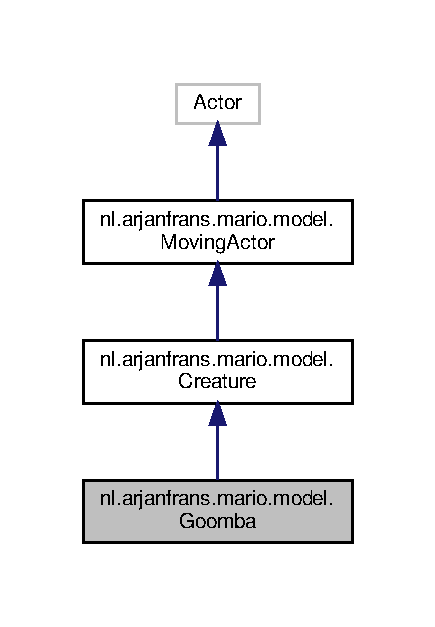
\includegraphics[width=209pt]{classnl_1_1arjanfrans_1_1mario_1_1model_1_1Goomba__inherit__graph}
\end{center}
\end{figure}


Collaboration diagram for nl.\+arjanfrans.\+mario.\+model.\+Goomba\+:
\nopagebreak
\begin{figure}[H]
\begin{center}
\leavevmode
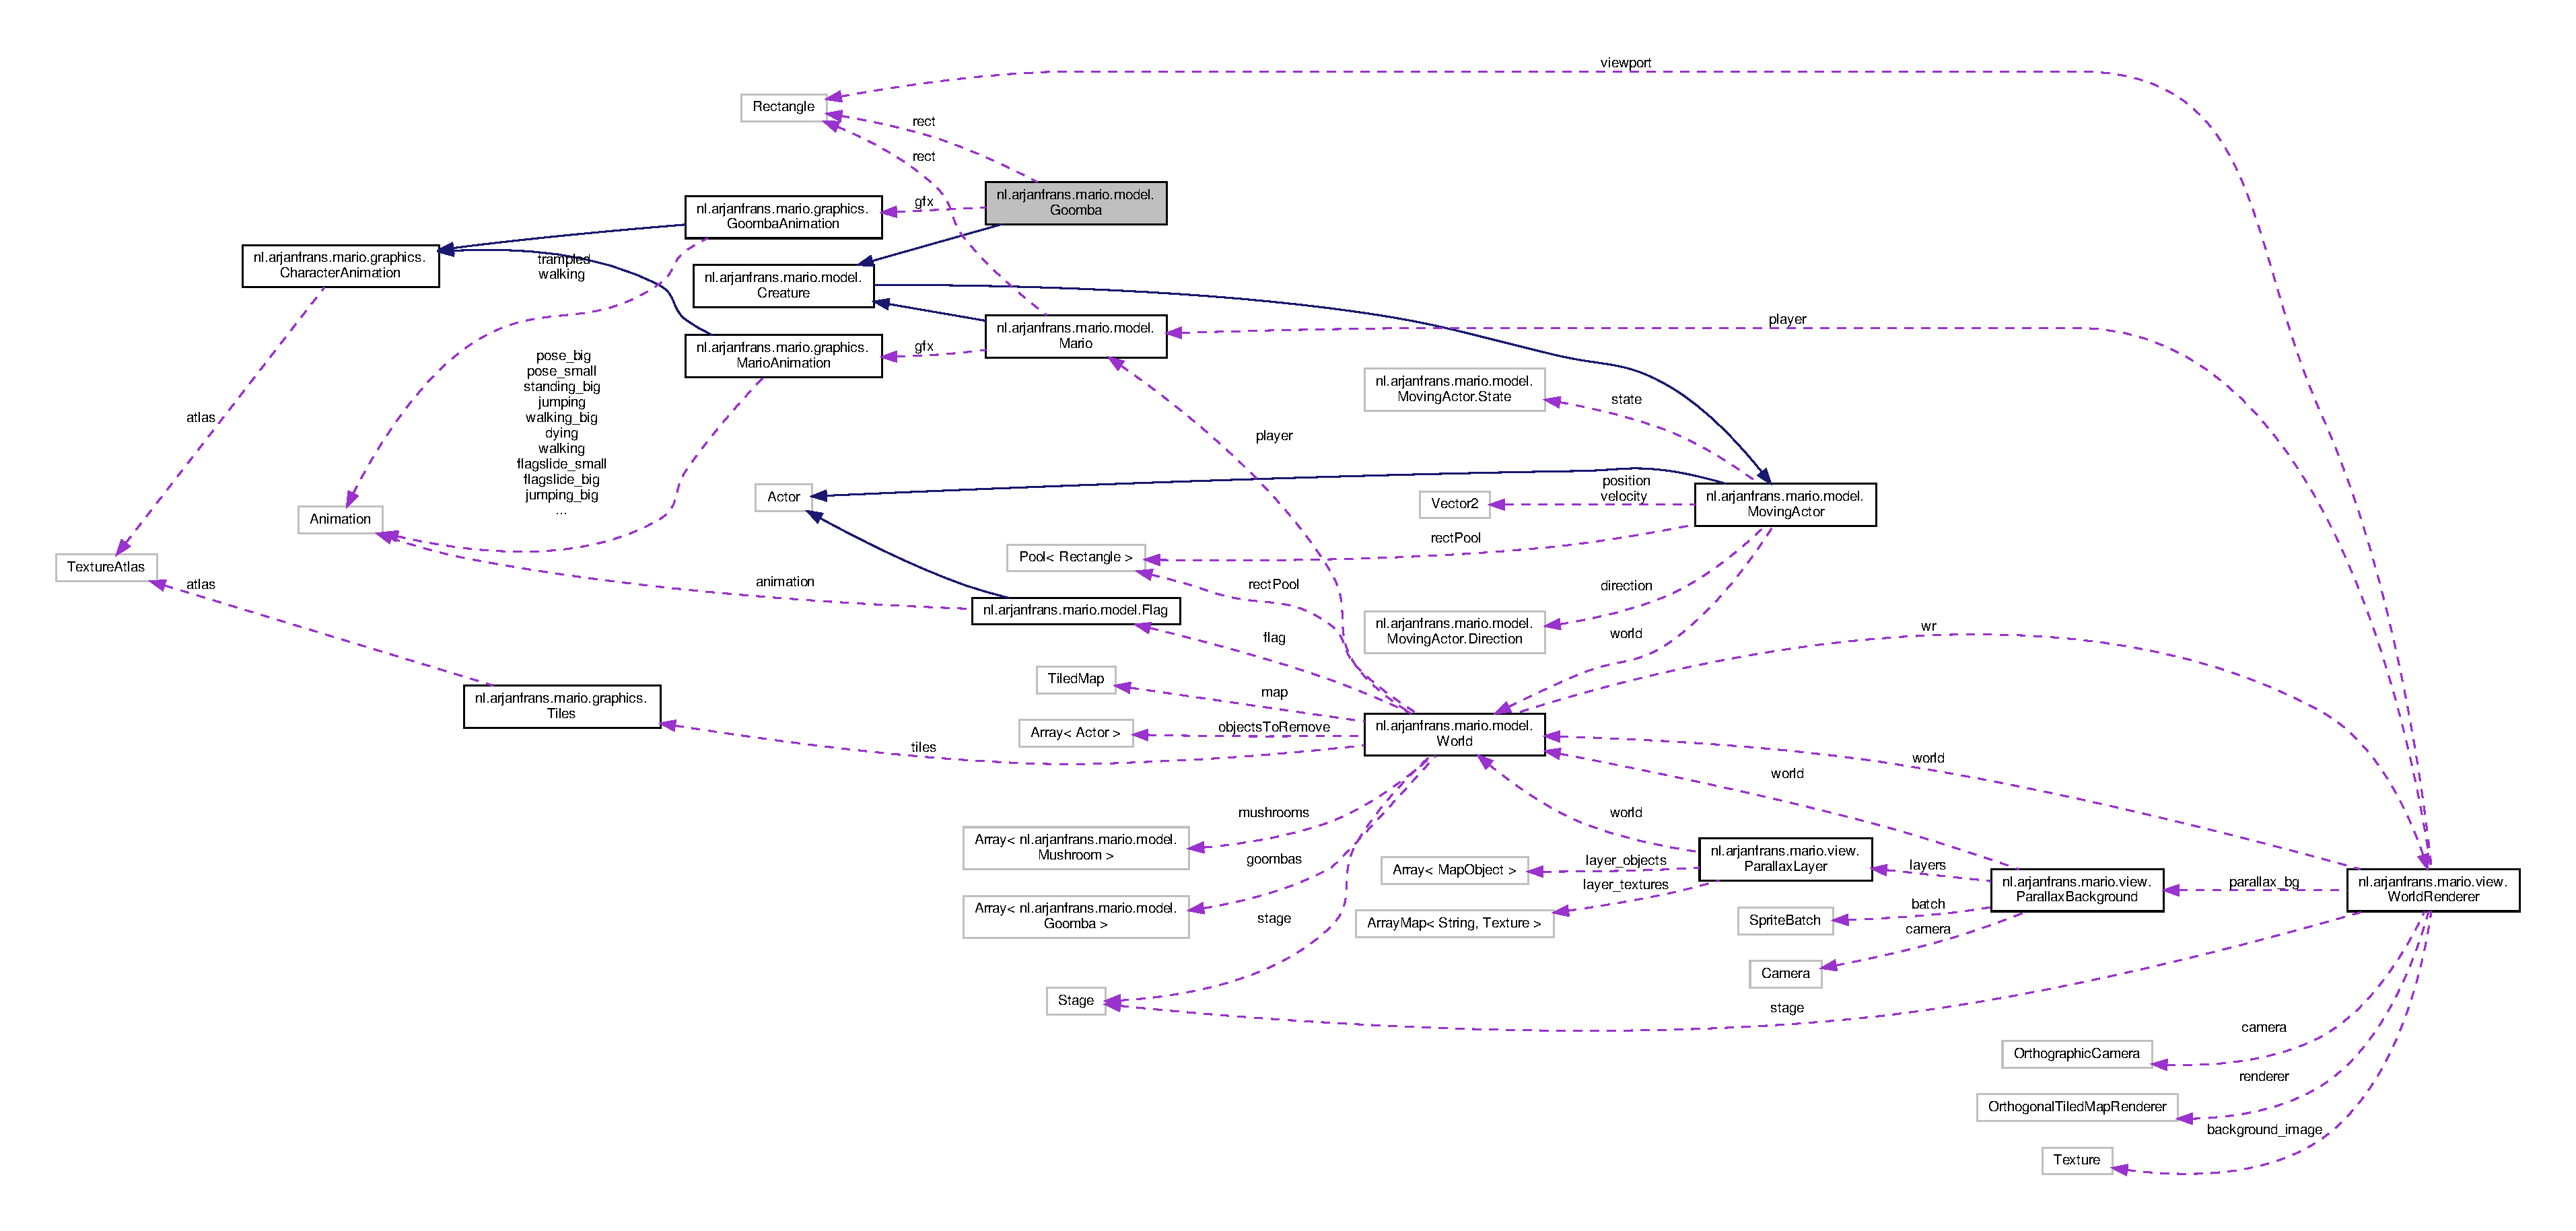
\includegraphics[width=350pt]{classnl_1_1arjanfrans_1_1mario_1_1model_1_1Goomba__coll__graph}
\end{center}
\end{figure}
\subsection*{Public Member Functions}
\begin{DoxyCompactItemize}
\item 
\hyperlink{classnl_1_1arjanfrans_1_1mario_1_1model_1_1Goomba_a71ffe3210dc6f4cfb0ea89ef714d5b2c}{Goomba} (\hyperlink{classnl_1_1arjanfrans_1_1mario_1_1model_1_1World}{World} world, float positionX, float positionY)
\begin{DoxyCompactList}\small\item\em Constructor method. \end{DoxyCompactList}\item 
void \hyperlink{classnl_1_1arjanfrans_1_1mario_1_1model_1_1Goomba_a36a01fff5535bd6629b4dd03ae452e63}{draw} (Batch batch, float parent\+Alpha)
\begin{DoxyCompactList}\small\item\em Draws the \hyperlink{classnl_1_1arjanfrans_1_1mario_1_1model_1_1Goomba}{Goomba} on the G\+UI. \end{DoxyCompactList}\item 
void \hyperlink{classnl_1_1arjanfrans_1_1mario_1_1model_1_1Goomba_ab0215022ef047cd9d82a8fd0447f4a38}{act} (float delta)
\begin{DoxyCompactList}\small\item\em Determines how the \hyperlink{classnl_1_1arjanfrans_1_1mario_1_1model_1_1Goomba}{Goomba} acts after each discrete time step. \end{DoxyCompactList}\item 
Animation \hyperlink{classnl_1_1arjanfrans_1_1mario_1_1model_1_1Goomba_a6d868ec59ecf46f1562a39ffe521e355}{get\+Animation} ()
\begin{DoxyCompactList}\small\item\em Gets the animation of this \hyperlink{classnl_1_1arjanfrans_1_1mario_1_1model_1_1Goomba}{Goomba}. \end{DoxyCompactList}\item 
\mbox{\Hypertarget{classnl_1_1arjanfrans_1_1mario_1_1model_1_1Goomba_a0167198d965a03dd35bbbf711962f02c}\label{classnl_1_1arjanfrans_1_1mario_1_1model_1_1Goomba_a0167198d965a03dd35bbbf711962f02c}} 
void \hyperlink{classnl_1_1arjanfrans_1_1mario_1_1model_1_1Goomba_a0167198d965a03dd35bbbf711962f02c}{dispose} ()
\begin{DoxyCompactList}\small\item\em Removes the \hyperlink{classnl_1_1arjanfrans_1_1mario_1_1model_1_1Goomba}{Goomba} from the world. \end{DoxyCompactList}\end{DoxyCompactItemize}
\subsection*{Protected Member Functions}
\begin{DoxyCompactItemize}
\item 
\mbox{\Hypertarget{classnl_1_1arjanfrans_1_1mario_1_1model_1_1Goomba_a76e5dd07d57bf351793acd2de5a5f901}\label{classnl_1_1arjanfrans_1_1mario_1_1model_1_1Goomba_a76e5dd07d57bf351793acd2de5a5f901}} 
void \hyperlink{classnl_1_1arjanfrans_1_1mario_1_1model_1_1Goomba_a76e5dd07d57bf351793acd2de5a5f901}{dead\+By\+Trample} ()
\begin{DoxyCompactList}\small\item\em \hyperlink{classnl_1_1arjanfrans_1_1mario_1_1model_1_1Goomba}{Goomba} dies by getting trampled. \end{DoxyCompactList}\item 
\mbox{\Hypertarget{classnl_1_1arjanfrans_1_1mario_1_1model_1_1Goomba_a494785b906ae8fcaf9057ecbc12ee55d}\label{classnl_1_1arjanfrans_1_1mario_1_1model_1_1Goomba_a494785b906ae8fcaf9057ecbc12ee55d}} 
void \hyperlink{classnl_1_1arjanfrans_1_1mario_1_1model_1_1Goomba_a494785b906ae8fcaf9057ecbc12ee55d}{die\+By\+Falling} ()
\begin{DoxyCompactList}\small\item\em \hyperlink{classnl_1_1arjanfrans_1_1mario_1_1model_1_1Goomba}{Goomba} dies by falling off the map. \end{DoxyCompactList}\item 
void \hyperlink{classnl_1_1arjanfrans_1_1mario_1_1model_1_1Goomba_a4582ee22090958c89e08267a2393c46c}{collision\+With\+Creature} ()
\begin{DoxyCompactList}\small\item\em Determines behaviour when \hyperlink{classnl_1_1arjanfrans_1_1mario_1_1model_1_1Goomba}{Goomba} collides with another creature. \end{DoxyCompactList}\item 
\mbox{\Hypertarget{classnl_1_1arjanfrans_1_1mario_1_1model_1_1Goomba_a47885ec93ca549c62176a931a46de7e6}\label{classnl_1_1arjanfrans_1_1mario_1_1model_1_1Goomba_a47885ec93ca549c62176a931a46de7e6}} 
void \hyperlink{classnl_1_1arjanfrans_1_1mario_1_1model_1_1Goomba_a47885ec93ca549c62176a931a46de7e6}{collision\+X\+Action} ()
\begin{DoxyCompactList}\small\item\em Determines behaviour of when \hyperlink{classnl_1_1arjanfrans_1_1mario_1_1model_1_1Goomba}{Goomba} collides with an object in the X direction. \end{DoxyCompactList}\end{DoxyCompactItemize}
\subsection*{Protected Attributes}
\begin{DoxyCompactItemize}
\item 
float \hyperlink{classnl_1_1arjanfrans_1_1mario_1_1model_1_1Goomba_a8cc5010ce400234e91ec1c13be0d8421}{max\+\_\+velocity} = 1f
\item 
\hyperlink{classnl_1_1arjanfrans_1_1mario_1_1graphics_1_1GoombaAnimation}{Goomba\+Animation} \hyperlink{classnl_1_1arjanfrans_1_1mario_1_1model_1_1Goomba_a936ff77c12f392ca3bf555f49b850e9e}{gfx} = new \hyperlink{classnl_1_1arjanfrans_1_1mario_1_1graphics_1_1GoombaAnimation}{Goomba\+Animation}()
\item 
Rectangle \hyperlink{classnl_1_1arjanfrans_1_1mario_1_1model_1_1Goomba_af4a69ae09f56588a52ee32b7228c21f6}{rect} = new Rectangle()
\end{DoxyCompactItemize}
\subsection*{Private Member Functions}
\begin{DoxyCompactItemize}
\item 
void \hyperlink{classnl_1_1arjanfrans_1_1mario_1_1model_1_1Goomba_a307cf941d782f3a0c2734eb56c1165da}{die\+By\+Trample} ()
\begin{DoxyCompactList}\small\item\em When \hyperlink{classnl_1_1arjanfrans_1_1mario_1_1model_1_1Goomba}{Goomba} dies by getting trampled. \end{DoxyCompactList}\end{DoxyCompactItemize}


\subsection{Detailed Description}
\hyperlink{classnl_1_1arjanfrans_1_1mario_1_1model_1_1Goomba}{Goomba} represents the \hyperlink{classnl_1_1arjanfrans_1_1mario_1_1model_1_1Goomba}{Goomba} enemies from the original \hyperlink{classnl_1_1arjanfrans_1_1mario_1_1model_1_1Mario}{Mario} game. 

\subsection{Constructor \& Destructor Documentation}
\mbox{\Hypertarget{classnl_1_1arjanfrans_1_1mario_1_1model_1_1Goomba_a71ffe3210dc6f4cfb0ea89ef714d5b2c}\label{classnl_1_1arjanfrans_1_1mario_1_1model_1_1Goomba_a71ffe3210dc6f4cfb0ea89ef714d5b2c}} 
\index{nl\+::arjanfrans\+::mario\+::model\+::\+Goomba@{nl\+::arjanfrans\+::mario\+::model\+::\+Goomba}!Goomba@{Goomba}}
\index{Goomba@{Goomba}!nl\+::arjanfrans\+::mario\+::model\+::\+Goomba@{nl\+::arjanfrans\+::mario\+::model\+::\+Goomba}}
\subsubsection{\texorpdfstring{Goomba()}{Goomba()}}
{\footnotesize\ttfamily nl.\+arjanfrans.\+mario.\+model.\+Goomba.\+Goomba (\begin{DoxyParamCaption}\item[{\hyperlink{classnl_1_1arjanfrans_1_1mario_1_1model_1_1World}{World}}]{world,  }\item[{float}]{positionX,  }\item[{float}]{positionY }\end{DoxyParamCaption})}



Constructor method. 

Method which initializes an instance of \hyperlink{classnl_1_1arjanfrans_1_1mario_1_1model_1_1Goomba}{Goomba} 
\begin{DoxyParams}{Parameters}
{\em world} & The world in which the \hyperlink{classnl_1_1arjanfrans_1_1mario_1_1model_1_1Goomba}{Goomba} will exist in \\
\hline
{\em positionX} & x coordinate of the position of the \hyperlink{classnl_1_1arjanfrans_1_1mario_1_1model_1_1Goomba}{Goomba} \\
\hline
{\em positionY} & y coordinate of the position of the \hyperlink{classnl_1_1arjanfrans_1_1mario_1_1model_1_1Goomba}{Goomba} \\
\hline
\end{DoxyParams}
\begin{DoxyReturn}{Returns}
An instance of \hyperlink{classnl_1_1arjanfrans_1_1mario_1_1model_1_1Goomba}{Goomba} 
\end{DoxyReturn}


\subsection{Member Function Documentation}
\mbox{\Hypertarget{classnl_1_1arjanfrans_1_1mario_1_1model_1_1Goomba_ab0215022ef047cd9d82a8fd0447f4a38}\label{classnl_1_1arjanfrans_1_1mario_1_1model_1_1Goomba_ab0215022ef047cd9d82a8fd0447f4a38}} 
\index{nl\+::arjanfrans\+::mario\+::model\+::\+Goomba@{nl\+::arjanfrans\+::mario\+::model\+::\+Goomba}!act@{act}}
\index{act@{act}!nl\+::arjanfrans\+::mario\+::model\+::\+Goomba@{nl\+::arjanfrans\+::mario\+::model\+::\+Goomba}}
\subsubsection{\texorpdfstring{act()}{act()}}
{\footnotesize\ttfamily void nl.\+arjanfrans.\+mario.\+model.\+Goomba.\+act (\begin{DoxyParamCaption}\item[{float}]{delta }\end{DoxyParamCaption})}



Determines how the \hyperlink{classnl_1_1arjanfrans_1_1mario_1_1model_1_1Goomba}{Goomba} acts after each discrete time step. 


\begin{DoxyParams}{Parameters}
{\em delta} & Float representing the change in time \\
\hline
\end{DoxyParams}
\mbox{\Hypertarget{classnl_1_1arjanfrans_1_1mario_1_1model_1_1Goomba_a4582ee22090958c89e08267a2393c46c}\label{classnl_1_1arjanfrans_1_1mario_1_1model_1_1Goomba_a4582ee22090958c89e08267a2393c46c}} 
\index{nl\+::arjanfrans\+::mario\+::model\+::\+Goomba@{nl\+::arjanfrans\+::mario\+::model\+::\+Goomba}!collision\+With\+Creature@{collision\+With\+Creature}}
\index{collision\+With\+Creature@{collision\+With\+Creature}!nl\+::arjanfrans\+::mario\+::model\+::\+Goomba@{nl\+::arjanfrans\+::mario\+::model\+::\+Goomba}}
\subsubsection{\texorpdfstring{collision\+With\+Creature()}{collisionWithCreature()}}
{\footnotesize\ttfamily void nl.\+arjanfrans.\+mario.\+model.\+Goomba.\+collision\+With\+Creature (\begin{DoxyParamCaption}{ }\end{DoxyParamCaption})\hspace{0.3cm}{\ttfamily [protected]}}



Determines behaviour when \hyperlink{classnl_1_1arjanfrans_1_1mario_1_1model_1_1Goomba}{Goomba} collides with another creature. 

Checks if this \hyperlink{classnl_1_1arjanfrans_1_1mario_1_1model_1_1Goomba}{Goomba} is colliding with any other \hyperlink{classnl_1_1arjanfrans_1_1mario_1_1model_1_1Goomba}{Goomba} in the world \mbox{\Hypertarget{classnl_1_1arjanfrans_1_1mario_1_1model_1_1Goomba_a307cf941d782f3a0c2734eb56c1165da}\label{classnl_1_1arjanfrans_1_1mario_1_1model_1_1Goomba_a307cf941d782f3a0c2734eb56c1165da}} 
\index{nl\+::arjanfrans\+::mario\+::model\+::\+Goomba@{nl\+::arjanfrans\+::mario\+::model\+::\+Goomba}!die\+By\+Trample@{die\+By\+Trample}}
\index{die\+By\+Trample@{die\+By\+Trample}!nl\+::arjanfrans\+::mario\+::model\+::\+Goomba@{nl\+::arjanfrans\+::mario\+::model\+::\+Goomba}}
\subsubsection{\texorpdfstring{die\+By\+Trample()}{dieByTrample()}}
{\footnotesize\ttfamily void nl.\+arjanfrans.\+mario.\+model.\+Goomba.\+die\+By\+Trample (\begin{DoxyParamCaption}{ }\end{DoxyParamCaption})\hspace{0.3cm}{\ttfamily [private]}}



When \hyperlink{classnl_1_1arjanfrans_1_1mario_1_1model_1_1Goomba}{Goomba} dies by getting trampled. 

A \hyperlink{classnl_1_1arjanfrans_1_1mario_1_1model_1_1Goomba}{Goomba} will die when getting trampled (\hyperlink{classnl_1_1arjanfrans_1_1mario_1_1model_1_1Mario}{Mario} steps on \hyperlink{classnl_1_1arjanfrans_1_1mario_1_1model_1_1Goomba}{Goomba}\textquotesingle{}s head). This results in the \hyperlink{classnl_1_1arjanfrans_1_1mario_1_1model_1_1Goomba}{Goomba} dying and being removed from the world \mbox{\Hypertarget{classnl_1_1arjanfrans_1_1mario_1_1model_1_1Goomba_a36a01fff5535bd6629b4dd03ae452e63}\label{classnl_1_1arjanfrans_1_1mario_1_1model_1_1Goomba_a36a01fff5535bd6629b4dd03ae452e63}} 
\index{nl\+::arjanfrans\+::mario\+::model\+::\+Goomba@{nl\+::arjanfrans\+::mario\+::model\+::\+Goomba}!draw@{draw}}
\index{draw@{draw}!nl\+::arjanfrans\+::mario\+::model\+::\+Goomba@{nl\+::arjanfrans\+::mario\+::model\+::\+Goomba}}
\subsubsection{\texorpdfstring{draw()}{draw()}}
{\footnotesize\ttfamily void nl.\+arjanfrans.\+mario.\+model.\+Goomba.\+draw (\begin{DoxyParamCaption}\item[{Batch}]{batch,  }\item[{float}]{parent\+Alpha }\end{DoxyParamCaption})}



Draws the \hyperlink{classnl_1_1arjanfrans_1_1mario_1_1model_1_1Goomba}{Goomba} on the G\+UI. 

Assists lib\+G\+DX in drawing the \hyperlink{classnl_1_1arjanfrans_1_1mario_1_1model_1_1Goomba}{Goomba} to a specified batch 
\begin{DoxyParams}{Parameters}
{\em batch} & The texture region where the \hyperlink{classnl_1_1arjanfrans_1_1mario_1_1model_1_1Goomba}{Goomba} is being drawn \\
\hline
{\em parent\+Alpha} & Not used \\
\hline
\end{DoxyParams}
\mbox{\Hypertarget{classnl_1_1arjanfrans_1_1mario_1_1model_1_1Goomba_a6d868ec59ecf46f1562a39ffe521e355}\label{classnl_1_1arjanfrans_1_1mario_1_1model_1_1Goomba_a6d868ec59ecf46f1562a39ffe521e355}} 
\index{nl\+::arjanfrans\+::mario\+::model\+::\+Goomba@{nl\+::arjanfrans\+::mario\+::model\+::\+Goomba}!get\+Animation@{get\+Animation}}
\index{get\+Animation@{get\+Animation}!nl\+::arjanfrans\+::mario\+::model\+::\+Goomba@{nl\+::arjanfrans\+::mario\+::model\+::\+Goomba}}
\subsubsection{\texorpdfstring{get\+Animation()}{getAnimation()}}
{\footnotesize\ttfamily Animation nl.\+arjanfrans.\+mario.\+model.\+Goomba.\+get\+Animation (\begin{DoxyParamCaption}{ }\end{DoxyParamCaption})}



Gets the animation of this \hyperlink{classnl_1_1arjanfrans_1_1mario_1_1model_1_1Goomba}{Goomba}. 

\begin{DoxyReturn}{Returns}
Animation object representing which animations the \hyperlink{classnl_1_1arjanfrans_1_1mario_1_1model_1_1Goomba}{Goomba} will play 
\end{DoxyReturn}


\subsection{Member Data Documentation}
\mbox{\Hypertarget{classnl_1_1arjanfrans_1_1mario_1_1model_1_1Goomba_a936ff77c12f392ca3bf555f49b850e9e}\label{classnl_1_1arjanfrans_1_1mario_1_1model_1_1Goomba_a936ff77c12f392ca3bf555f49b850e9e}} 
\index{nl\+::arjanfrans\+::mario\+::model\+::\+Goomba@{nl\+::arjanfrans\+::mario\+::model\+::\+Goomba}!gfx@{gfx}}
\index{gfx@{gfx}!nl\+::arjanfrans\+::mario\+::model\+::\+Goomba@{nl\+::arjanfrans\+::mario\+::model\+::\+Goomba}}
\subsubsection{\texorpdfstring{gfx}{gfx}}
{\footnotesize\ttfamily \hyperlink{classnl_1_1arjanfrans_1_1mario_1_1graphics_1_1GoombaAnimation}{Goomba\+Animation} nl.\+arjanfrans.\+mario.\+model.\+Goomba.\+gfx = new \hyperlink{classnl_1_1arjanfrans_1_1mario_1_1graphics_1_1GoombaAnimation}{Goomba\+Animation}()\hspace{0.3cm}{\ttfamily [protected]}}

Animations of \hyperlink{classnl_1_1arjanfrans_1_1mario_1_1model_1_1Goomba}{Goomba} \mbox{\Hypertarget{classnl_1_1arjanfrans_1_1mario_1_1model_1_1Goomba_a8cc5010ce400234e91ec1c13be0d8421}\label{classnl_1_1arjanfrans_1_1mario_1_1model_1_1Goomba_a8cc5010ce400234e91ec1c13be0d8421}} 
\index{nl\+::arjanfrans\+::mario\+::model\+::\+Goomba@{nl\+::arjanfrans\+::mario\+::model\+::\+Goomba}!max\+\_\+velocity@{max\+\_\+velocity}}
\index{max\+\_\+velocity@{max\+\_\+velocity}!nl\+::arjanfrans\+::mario\+::model\+::\+Goomba@{nl\+::arjanfrans\+::mario\+::model\+::\+Goomba}}
\subsubsection{\texorpdfstring{max\+\_\+velocity}{max\_velocity}}
{\footnotesize\ttfamily float nl.\+arjanfrans.\+mario.\+model.\+Goomba.\+max\+\_\+velocity = 1f\hspace{0.3cm}{\ttfamily [protected]}}

Maximum velocity of \hyperlink{classnl_1_1arjanfrans_1_1mario_1_1model_1_1Goomba}{Goomba} \mbox{\Hypertarget{classnl_1_1arjanfrans_1_1mario_1_1model_1_1Goomba_af4a69ae09f56588a52ee32b7228c21f6}\label{classnl_1_1arjanfrans_1_1mario_1_1model_1_1Goomba_af4a69ae09f56588a52ee32b7228c21f6}} 
\index{nl\+::arjanfrans\+::mario\+::model\+::\+Goomba@{nl\+::arjanfrans\+::mario\+::model\+::\+Goomba}!rect@{rect}}
\index{rect@{rect}!nl\+::arjanfrans\+::mario\+::model\+::\+Goomba@{nl\+::arjanfrans\+::mario\+::model\+::\+Goomba}}
\subsubsection{\texorpdfstring{rect}{rect}}
{\footnotesize\ttfamily Rectangle nl.\+arjanfrans.\+mario.\+model.\+Goomba.\+rect = new Rectangle()\hspace{0.3cm}{\ttfamily [protected]}}

Rectangle object surrounding the \hyperlink{classnl_1_1arjanfrans_1_1mario_1_1model_1_1Goomba}{Goomba} 

The documentation for this class was generated from the following file\+:\begin{DoxyCompactItemize}
\item 
core/src/nl/arjanfrans/mario/model/\hyperlink{Goomba_8java}{Goomba.\+java}\end{DoxyCompactItemize}

\hypertarget{classnl_1_1arjanfrans_1_1mario_1_1graphics_1_1GoombaAnimation}{}\section{nl.\+arjanfrans.\+mario.\+graphics.\+Goomba\+Animation Class Reference}
\label{classnl_1_1arjanfrans_1_1mario_1_1graphics_1_1GoombaAnimation}\index{nl.\+arjanfrans.\+mario.\+graphics.\+Goomba\+Animation@{nl.\+arjanfrans.\+mario.\+graphics.\+Goomba\+Animation}}


This is a class that implements the abstract class, \hyperlink{classnl_1_1arjanfrans_1_1mario_1_1graphics_1_1CharacterAnimation}{Character\+Animation}, specifically for the animation of the Goomba character.  




Inheritance diagram for nl.\+arjanfrans.\+mario.\+graphics.\+Goomba\+Animation\+:
\nopagebreak
\begin{figure}[H]
\begin{center}
\leavevmode
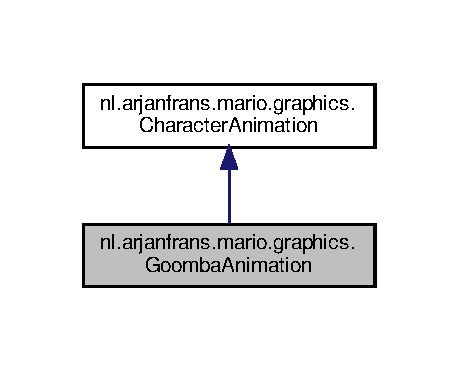
\includegraphics[width=220pt]{classnl_1_1arjanfrans_1_1mario_1_1graphics_1_1GoombaAnimation__inherit__graph}
\end{center}
\end{figure}


Collaboration diagram for nl.\+arjanfrans.\+mario.\+graphics.\+Goomba\+Animation\+:
\nopagebreak
\begin{figure}[H]
\begin{center}
\leavevmode
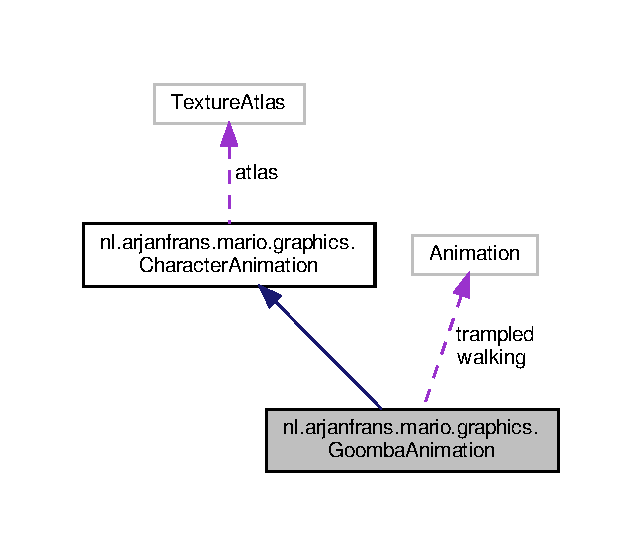
\includegraphics[width=308pt]{classnl_1_1arjanfrans_1_1mario_1_1graphics_1_1GoombaAnimation__coll__graph}
\end{center}
\end{figure}
\subsection*{Public Member Functions}
\begin{DoxyCompactItemize}
\item 
\hyperlink{classnl_1_1arjanfrans_1_1mario_1_1graphics_1_1GoombaAnimation_a992fa17bfdfa40dea72f5f4453c821a6}{Goomba\+Animation} ()
\begin{DoxyCompactList}\small\item\em Constructor method for \hyperlink{classnl_1_1arjanfrans_1_1mario_1_1graphics_1_1GoombaAnimation}{Goomba\+Animation}. \end{DoxyCompactList}\item 
Animation \hyperlink{classnl_1_1arjanfrans_1_1mario_1_1graphics_1_1GoombaAnimation_a10532017e2baab74a43750e906a8bcdc}{get\+Animation} (State state)
\begin{DoxyCompactList}\small\item\em A method meant to retrieve a Goomba animation based on the Goomba\textquotesingle{}s state. \end{DoxyCompactList}\item 
Vector2 \hyperlink{classnl_1_1arjanfrans_1_1mario_1_1graphics_1_1GoombaAnimation_a49e10158e12095415ed637bc2092f546}{get\+Dimensions} (State state)
\begin{DoxyCompactList}\small\item\em A method meant to retrieve the dimensions of a Goomba animation based on the Goomba\textquotesingle{}s state. \end{DoxyCompactList}\end{DoxyCompactItemize}
\subsection*{Private Attributes}
\begin{DoxyCompactItemize}
\item 
\mbox{\Hypertarget{classnl_1_1arjanfrans_1_1mario_1_1graphics_1_1GoombaAnimation_a292bc268550534422c4ea255a257f586}\label{classnl_1_1arjanfrans_1_1mario_1_1graphics_1_1GoombaAnimation_a292bc268550534422c4ea255a257f586}} 
Animation {\bfseries walking}
\item 
\mbox{\Hypertarget{classnl_1_1arjanfrans_1_1mario_1_1graphics_1_1GoombaAnimation_a54a746c4e2d84985e07cc749077144f1}\label{classnl_1_1arjanfrans_1_1mario_1_1graphics_1_1GoombaAnimation_a54a746c4e2d84985e07cc749077144f1}} 
Animation {\bfseries trampled}
\end{DoxyCompactItemize}
\subsection*{Additional Inherited Members}


\subsection{Detailed Description}
This is a class that implements the abstract class, \hyperlink{classnl_1_1arjanfrans_1_1mario_1_1graphics_1_1CharacterAnimation}{Character\+Animation}, specifically for the animation of the Goomba character. 

\subsection{Constructor \& Destructor Documentation}
\mbox{\Hypertarget{classnl_1_1arjanfrans_1_1mario_1_1graphics_1_1GoombaAnimation_a992fa17bfdfa40dea72f5f4453c821a6}\label{classnl_1_1arjanfrans_1_1mario_1_1graphics_1_1GoombaAnimation_a992fa17bfdfa40dea72f5f4453c821a6}} 
\index{nl\+::arjanfrans\+::mario\+::graphics\+::\+Goomba\+Animation@{nl\+::arjanfrans\+::mario\+::graphics\+::\+Goomba\+Animation}!Goomba\+Animation@{Goomba\+Animation}}
\index{Goomba\+Animation@{Goomba\+Animation}!nl\+::arjanfrans\+::mario\+::graphics\+::\+Goomba\+Animation@{nl\+::arjanfrans\+::mario\+::graphics\+::\+Goomba\+Animation}}
\subsubsection{\texorpdfstring{Goomba\+Animation()}{GoombaAnimation()}}
{\footnotesize\ttfamily nl.\+arjanfrans.\+mario.\+graphics.\+Goomba\+Animation.\+Goomba\+Animation (\begin{DoxyParamCaption}{ }\end{DoxyParamCaption})}



Constructor method for \hyperlink{classnl_1_1arjanfrans_1_1mario_1_1graphics_1_1GoombaAnimation}{Goomba\+Animation}. 

Method which initializes an instance of \hyperlink{classnl_1_1arjanfrans_1_1mario_1_1graphics_1_1GoombaAnimation}{Goomba\+Animation}. \begin{DoxyReturn}{Returns}
An instance of \hyperlink{classnl_1_1arjanfrans_1_1mario_1_1graphics_1_1GoombaAnimation}{Goomba\+Animation} 
\end{DoxyReturn}


\subsection{Member Function Documentation}
\mbox{\Hypertarget{classnl_1_1arjanfrans_1_1mario_1_1graphics_1_1GoombaAnimation_a10532017e2baab74a43750e906a8bcdc}\label{classnl_1_1arjanfrans_1_1mario_1_1graphics_1_1GoombaAnimation_a10532017e2baab74a43750e906a8bcdc}} 
\index{nl\+::arjanfrans\+::mario\+::graphics\+::\+Goomba\+Animation@{nl\+::arjanfrans\+::mario\+::graphics\+::\+Goomba\+Animation}!get\+Animation@{get\+Animation}}
\index{get\+Animation@{get\+Animation}!nl\+::arjanfrans\+::mario\+::graphics\+::\+Goomba\+Animation@{nl\+::arjanfrans\+::mario\+::graphics\+::\+Goomba\+Animation}}
\subsubsection{\texorpdfstring{get\+Animation()}{getAnimation()}}
{\footnotesize\ttfamily Animation nl.\+arjanfrans.\+mario.\+graphics.\+Goomba\+Animation.\+get\+Animation (\begin{DoxyParamCaption}\item[{State}]{state }\end{DoxyParamCaption})}



A method meant to retrieve a Goomba animation based on the Goomba\textquotesingle{}s state. 


\begin{DoxyParams}{Parameters}
{\em state} & -\/ the state of the Goomba, refers to the State enum class \\
\hline
\end{DoxyParams}
\begin{DoxyReturn}{Returns}
An instance of Animation 
\end{DoxyReturn}
\mbox{\Hypertarget{classnl_1_1arjanfrans_1_1mario_1_1graphics_1_1GoombaAnimation_a49e10158e12095415ed637bc2092f546}\label{classnl_1_1arjanfrans_1_1mario_1_1graphics_1_1GoombaAnimation_a49e10158e12095415ed637bc2092f546}} 
\index{nl\+::arjanfrans\+::mario\+::graphics\+::\+Goomba\+Animation@{nl\+::arjanfrans\+::mario\+::graphics\+::\+Goomba\+Animation}!get\+Dimensions@{get\+Dimensions}}
\index{get\+Dimensions@{get\+Dimensions}!nl\+::arjanfrans\+::mario\+::graphics\+::\+Goomba\+Animation@{nl\+::arjanfrans\+::mario\+::graphics\+::\+Goomba\+Animation}}
\subsubsection{\texorpdfstring{get\+Dimensions()}{getDimensions()}}
{\footnotesize\ttfamily Vector2 nl.\+arjanfrans.\+mario.\+graphics.\+Goomba\+Animation.\+get\+Dimensions (\begin{DoxyParamCaption}\item[{State}]{state }\end{DoxyParamCaption})}



A method meant to retrieve the dimensions of a Goomba animation based on the Goomba\textquotesingle{}s state. 


\begin{DoxyParams}{Parameters}
{\em state} & -\/ the state of the Goomba, refers to the State enum class. \\
\hline
\end{DoxyParams}
\begin{DoxyReturn}{Returns}
An instance of Vector2. 
\end{DoxyReturn}


The documentation for this class was generated from the following file\+:\begin{DoxyCompactItemize}
\item 
core/src/nl/arjanfrans/mario/graphics/Goomba\+Animation.\+java\end{DoxyCompactItemize}

\hypertarget{classnl_1_1arjanfrans_1_1mario_1_1model_1_1Item}{}\section{nl.\+arjanfrans.\+mario.\+model.\+Item Class Reference}
\label{classnl_1_1arjanfrans_1_1mario_1_1model_1_1Item}\index{nl.\+arjanfrans.\+mario.\+model.\+Item@{nl.\+arjanfrans.\+mario.\+model.\+Item}}


Represents any item in game.  




Inheritance diagram for nl.\+arjanfrans.\+mario.\+model.\+Item\+:\nopagebreak
\begin{figure}[H]
\begin{center}
\leavevmode
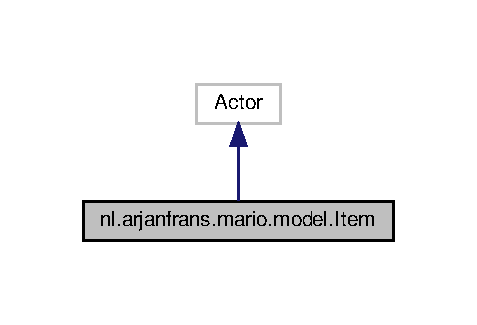
\includegraphics[width=229pt]{classnl_1_1arjanfrans_1_1mario_1_1model_1_1Item__inherit__graph}
\end{center}
\end{figure}


Collaboration diagram for nl.\+arjanfrans.\+mario.\+model.\+Item\+:
\nopagebreak
\begin{figure}[H]
\begin{center}
\leavevmode
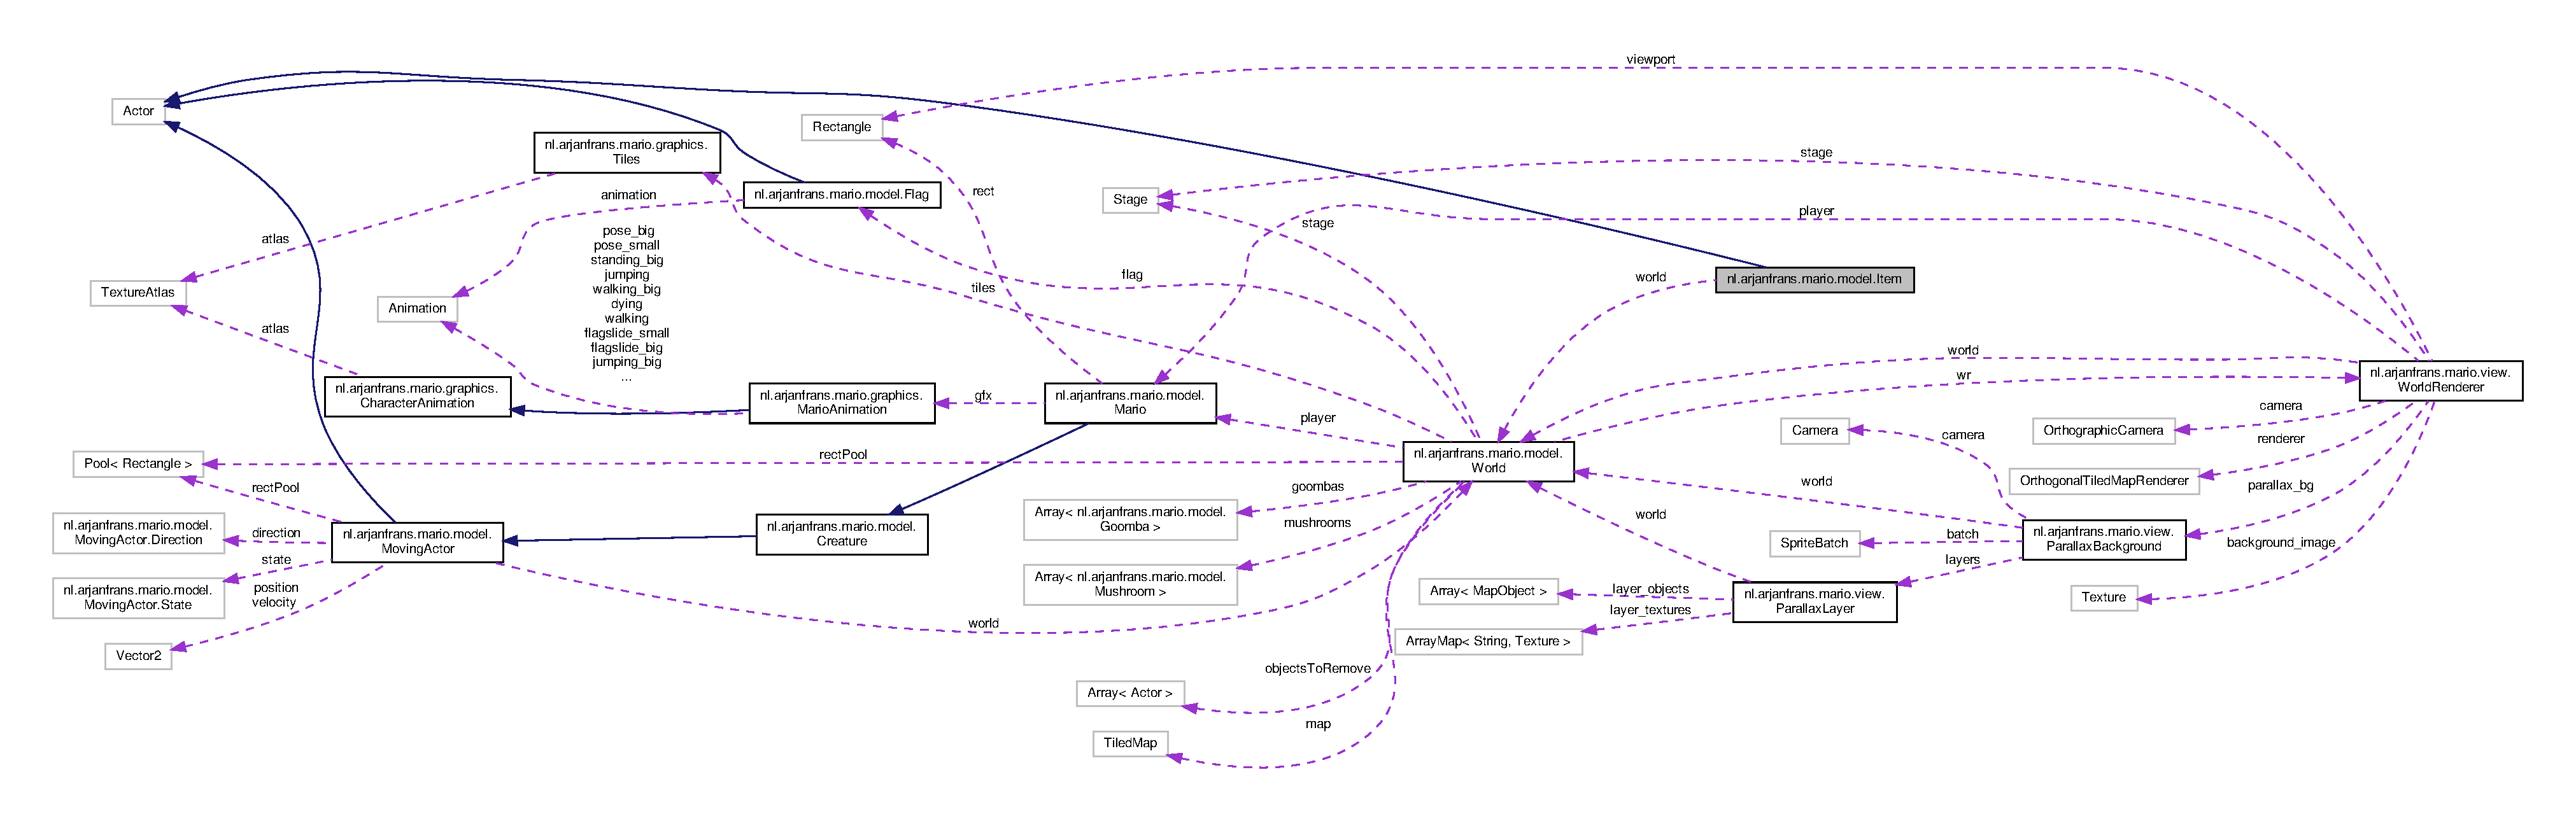
\includegraphics[width=350pt]{classnl_1_1arjanfrans_1_1mario_1_1model_1_1Item__coll__graph}
\end{center}
\end{figure}
\subsection*{Public Member Functions}
\begin{DoxyCompactItemize}
\item 
\hyperlink{classnl_1_1arjanfrans_1_1mario_1_1model_1_1Item_ae2c1344d50ddfa3e22fca0f1afa7f31f}{Item} (\hyperlink{classnl_1_1arjanfrans_1_1mario_1_1model_1_1World}{World} \hyperlink{classnl_1_1arjanfrans_1_1mario_1_1model_1_1Item_ae5d6d1a768987daac29679cf194ee95d}{world}, boolean visible)
\begin{DoxyCompactList}\small\item\em Constructor method. \end{DoxyCompactList}\end{DoxyCompactItemize}
\subsection*{Protected Attributes}
\begin{DoxyCompactItemize}
\item 
\hyperlink{classnl_1_1arjanfrans_1_1mario_1_1model_1_1World}{World} \hyperlink{classnl_1_1arjanfrans_1_1mario_1_1model_1_1Item_ae5d6d1a768987daac29679cf194ee95d}{world}
\end{DoxyCompactItemize}


\subsection{Detailed Description}
Represents any item in game. 

\subsection{Constructor \& Destructor Documentation}
\mbox{\Hypertarget{classnl_1_1arjanfrans_1_1mario_1_1model_1_1Item_ae2c1344d50ddfa3e22fca0f1afa7f31f}\label{classnl_1_1arjanfrans_1_1mario_1_1model_1_1Item_ae2c1344d50ddfa3e22fca0f1afa7f31f}} 
\index{nl\+::arjanfrans\+::mario\+::model\+::\+Item@{nl\+::arjanfrans\+::mario\+::model\+::\+Item}!Item@{Item}}
\index{Item@{Item}!nl\+::arjanfrans\+::mario\+::model\+::\+Item@{nl\+::arjanfrans\+::mario\+::model\+::\+Item}}
\subsubsection{\texorpdfstring{Item()}{Item()}}
{\footnotesize\ttfamily nl.\+arjanfrans.\+mario.\+model.\+Item.\+Item (\begin{DoxyParamCaption}\item[{\hyperlink{classnl_1_1arjanfrans_1_1mario_1_1model_1_1World}{World}}]{world,  }\item[{boolean}]{visible }\end{DoxyParamCaption})}



Constructor method. 

Method which initializes an instance of \hyperlink{classnl_1_1arjanfrans_1_1mario_1_1model_1_1Item}{Item} 
\begin{DoxyParams}{Parameters}
{\em world} & The world in which the \hyperlink{classnl_1_1arjanfrans_1_1mario_1_1model_1_1Goomba}{Goomba} will exist in \\
\hline
{\em visible} & If the item is visible or not \\
\hline
\end{DoxyParams}
\begin{DoxyReturn}{Returns}
An instance of \hyperlink{classnl_1_1arjanfrans_1_1mario_1_1model_1_1Item}{Item} 
\end{DoxyReturn}


\subsection{Member Data Documentation}
\mbox{\Hypertarget{classnl_1_1arjanfrans_1_1mario_1_1model_1_1Item_ae5d6d1a768987daac29679cf194ee95d}\label{classnl_1_1arjanfrans_1_1mario_1_1model_1_1Item_ae5d6d1a768987daac29679cf194ee95d}} 
\index{nl\+::arjanfrans\+::mario\+::model\+::\+Item@{nl\+::arjanfrans\+::mario\+::model\+::\+Item}!world@{world}}
\index{world@{world}!nl\+::arjanfrans\+::mario\+::model\+::\+Item@{nl\+::arjanfrans\+::mario\+::model\+::\+Item}}
\subsubsection{\texorpdfstring{world}{world}}
{\footnotesize\ttfamily \hyperlink{classnl_1_1arjanfrans_1_1mario_1_1model_1_1World}{World} nl.\+arjanfrans.\+mario.\+model.\+Item.\+world\hspace{0.3cm}{\ttfamily [protected]}}

The world in which the item exists 

The documentation for this class was generated from the following file\+:\begin{DoxyCompactItemize}
\item 
core/src/nl/arjanfrans/mario/model/\hyperlink{Item_8java}{Item.\+java}\end{DoxyCompactItemize}

\hypertarget{classnl_1_1arjanfrans_1_1mario_1_1model_1_1Mario}{}\section{nl.\+arjanfrans.\+mario.\+model.\+Mario Class Reference}
\label{classnl_1_1arjanfrans_1_1mario_1_1model_1_1Mario}\index{nl.\+arjanfrans.\+mario.\+model.\+Mario@{nl.\+arjanfrans.\+mario.\+model.\+Mario}}


Represents the playable character in the game.  




Inheritance diagram for nl.\+arjanfrans.\+mario.\+model.\+Mario\+:
\nopagebreak
\begin{figure}[H]
\begin{center}
\leavevmode
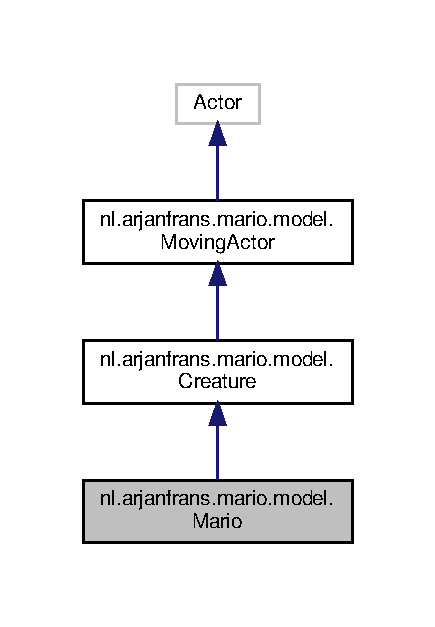
\includegraphics[width=209pt]{classnl_1_1arjanfrans_1_1mario_1_1model_1_1Mario__inherit__graph}
\end{center}
\end{figure}


Collaboration diagram for nl.\+arjanfrans.\+mario.\+model.\+Mario\+:
\nopagebreak
\begin{figure}[H]
\begin{center}
\leavevmode
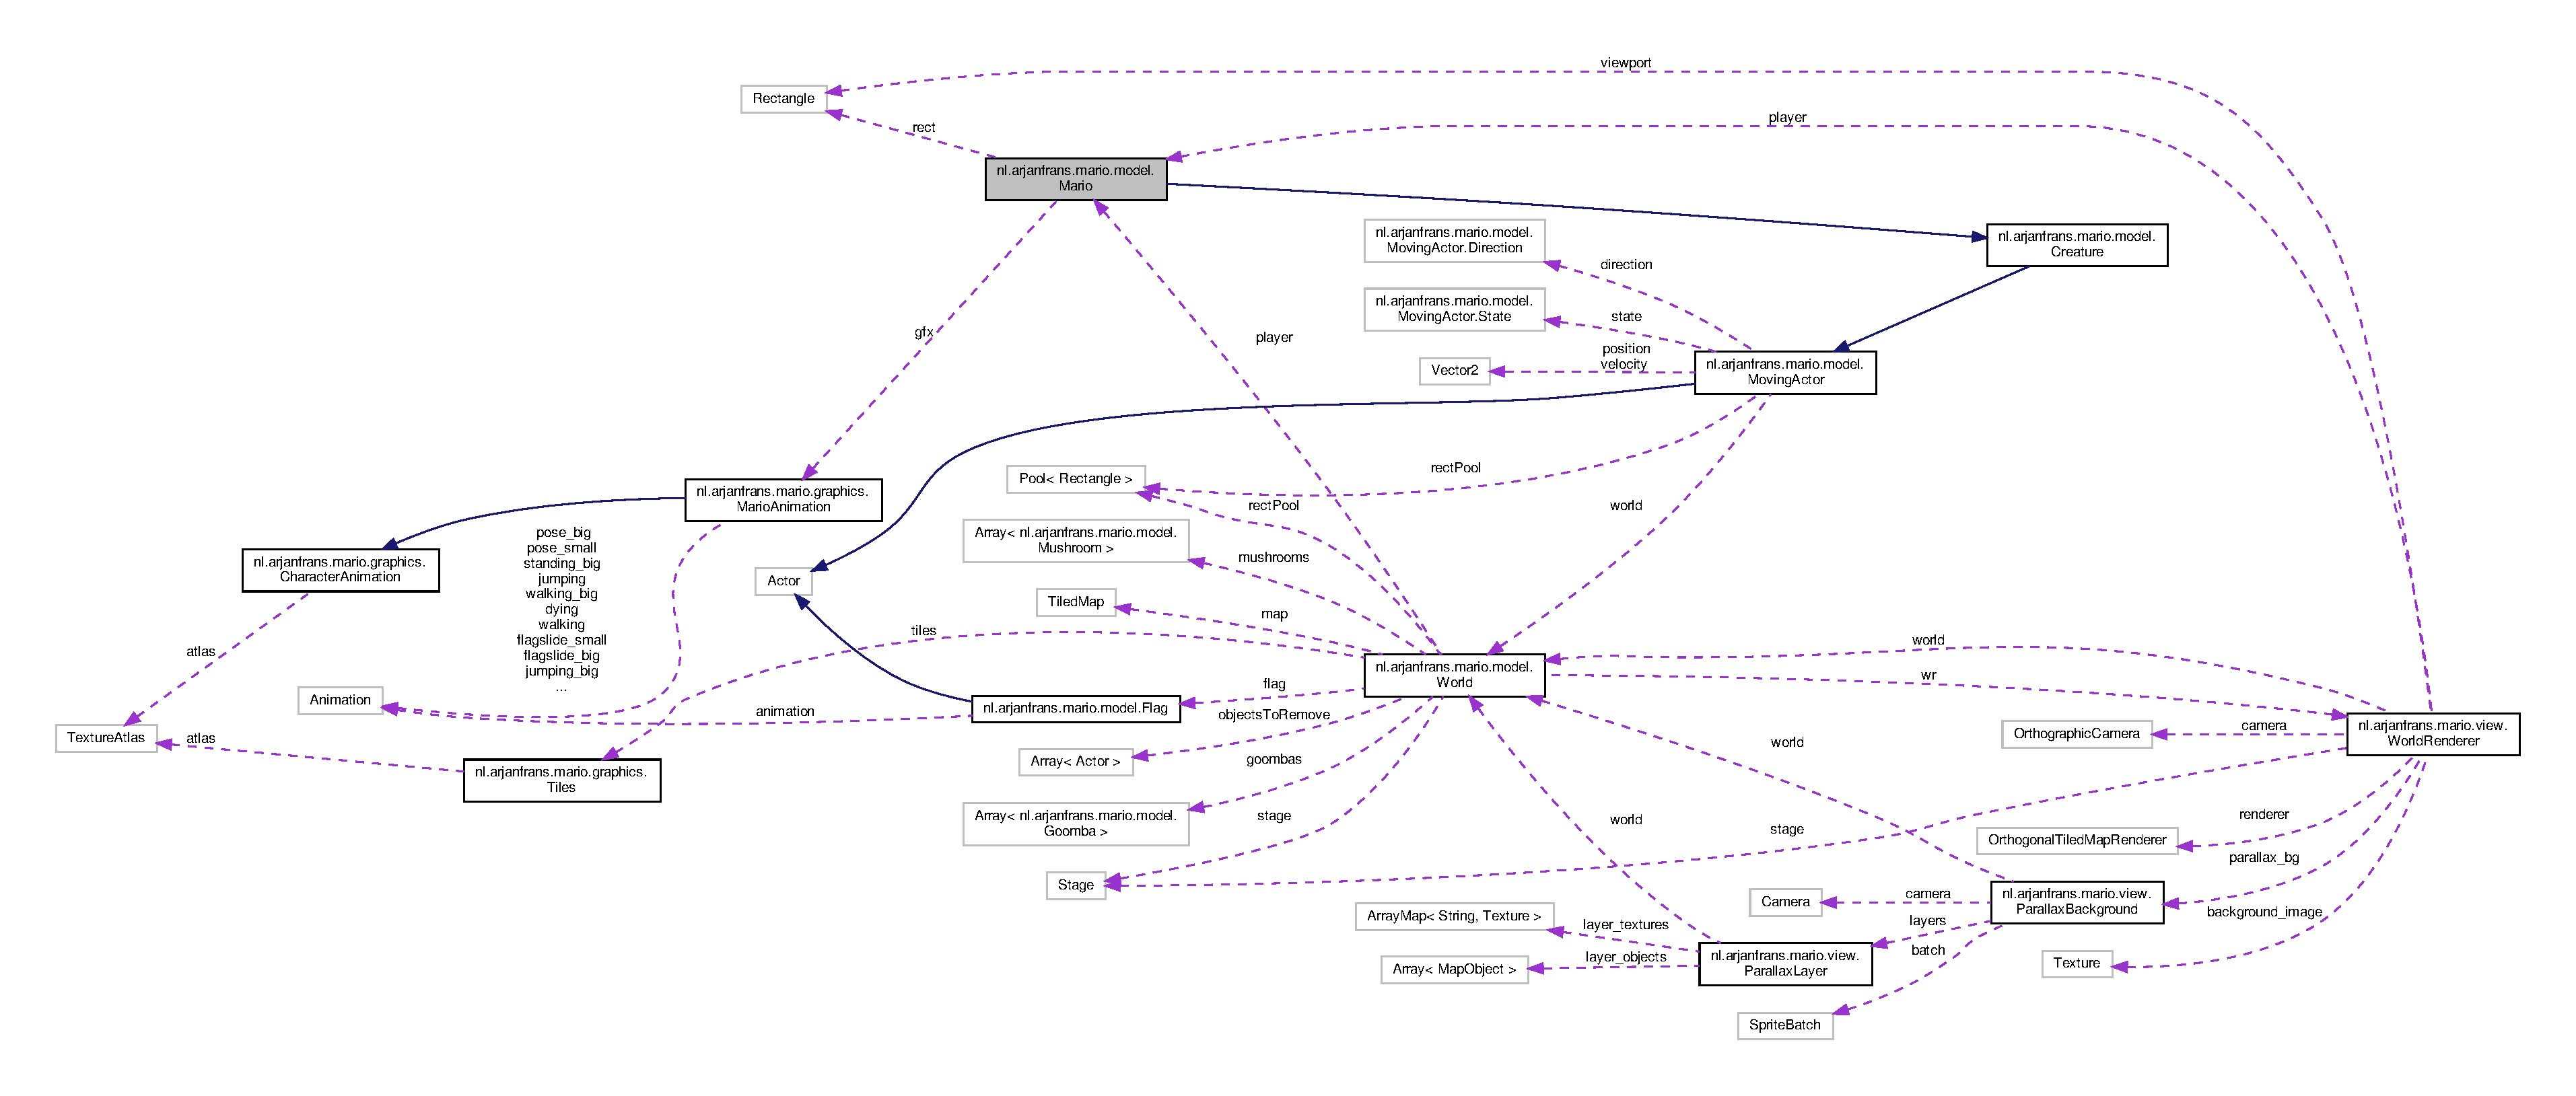
\includegraphics[width=350pt]{classnl_1_1arjanfrans_1_1mario_1_1model_1_1Mario__coll__graph}
\end{center}
\end{figure}
\subsection*{Public Member Functions}
\begin{DoxyCompactItemize}
\item 
\hyperlink{classnl_1_1arjanfrans_1_1mario_1_1model_1_1Mario_a3e3683dae8285b1bb0608d493b9b532a}{Mario} (\hyperlink{classnl_1_1arjanfrans_1_1mario_1_1model_1_1World}{World} world, float positionX, float positionY)
\begin{DoxyCompactList}\small\item\em Constructor method. \end{DoxyCompactList}\item 
void \hyperlink{classnl_1_1arjanfrans_1_1mario_1_1model_1_1Mario_a8e22f381330317da3aca016f4713f88a}{capture\+Flag} (\hyperlink{classnl_1_1arjanfrans_1_1mario_1_1model_1_1Flag}{Flag} flag, float endX, float endY)
\begin{DoxyCompactList}\small\item\em Behaviour when \hyperlink{classnl_1_1arjanfrans_1_1mario_1_1model_1_1Mario}{Mario} interacts with the flag pole (finishes the game) \end{DoxyCompactList}\item 
void \hyperlink{classnl_1_1arjanfrans_1_1mario_1_1model_1_1Mario_a231319aab3b67229e23c0ff4510c5239}{act} (float delta)
\begin{DoxyCompactList}\small\item\em Controls \hyperlink{classnl_1_1arjanfrans_1_1mario_1_1model_1_1Mario}{Mario}\textquotesingle{}s movement after each discrete time step. \end{DoxyCompactList}\item 
void \hyperlink{classnl_1_1arjanfrans_1_1mario_1_1model_1_1Mario_a50937f347ddf9eb8f114ad78e57e559c}{draw} (Batch batch, float parent\+Alpha)
\begin{DoxyCompactList}\small\item\em Draws \hyperlink{classnl_1_1arjanfrans_1_1mario_1_1model_1_1Mario}{Mario} on the G\+UI. \end{DoxyCompactList}\item 
Animation \hyperlink{classnl_1_1arjanfrans_1_1mario_1_1model_1_1Mario_a73c861a72b4a0ec8c7e87da0da5dac47}{get\+Animation} ()
\begin{DoxyCompactList}\small\item\em Returns \hyperlink{classnl_1_1arjanfrans_1_1mario_1_1model_1_1Mario}{Mario}\textquotesingle{}s animations. \end{DoxyCompactList}\item 
\mbox{\Hypertarget{classnl_1_1arjanfrans_1_1mario_1_1model_1_1Mario_a0a0c01da34e063939f6d50c43c8edda7}\label{classnl_1_1arjanfrans_1_1mario_1_1model_1_1Mario_a0a0c01da34e063939f6d50c43c8edda7}} 
void \hyperlink{classnl_1_1arjanfrans_1_1mario_1_1model_1_1Mario_a0a0c01da34e063939f6d50c43c8edda7}{dispose} ()
\begin{DoxyCompactList}\small\item\em Removes \hyperlink{classnl_1_1arjanfrans_1_1mario_1_1model_1_1Mario}{Mario} from the G\+UI. \end{DoxyCompactList}\item 
void \hyperlink{classnl_1_1arjanfrans_1_1mario_1_1model_1_1Mario_a4ff385372dd5b42110839b1c3a92e0c4}{set\+Immume} (boolean \hyperlink{classnl_1_1arjanfrans_1_1mario_1_1model_1_1Mario_a09b83e0286895f31f33418883c06ce01}{immume})
\begin{DoxyCompactList}\small\item\em Sets \hyperlink{classnl_1_1arjanfrans_1_1mario_1_1model_1_1Mario}{Mario}\textquotesingle{}s immune status. \end{DoxyCompactList}\item 
void \hyperlink{classnl_1_1arjanfrans_1_1mario_1_1model_1_1Mario_a4d82e5956168d3222d122854a17300dd}{move} (Direction dir)
\begin{DoxyCompactList}\small\item\em Sets \hyperlink{classnl_1_1arjanfrans_1_1mario_1_1model_1_1Mario}{Mario}\textquotesingle{}s velocity and direction to be in the direction of the specified movement. \end{DoxyCompactList}\item 
boolean \hyperlink{classnl_1_1arjanfrans_1_1mario_1_1model_1_1Mario_a3c4265e4764640c191e8177975feaf53}{is\+Controls\+Enabled} ()
\begin{DoxyCompactList}\small\item\em Returns whether the user has control of \hyperlink{classnl_1_1arjanfrans_1_1mario_1_1model_1_1Mario}{Mario}. \end{DoxyCompactList}\item 
void \hyperlink{classnl_1_1arjanfrans_1_1mario_1_1model_1_1Mario_aa396b035c909e03417db5f201d894e2f}{set\+Controls\+Enabled} (boolean \hyperlink{classnl_1_1arjanfrans_1_1mario_1_1model_1_1Mario_a5274108ef60b357abdca2e64b6378d58}{controls\+Enabled})
\begin{DoxyCompactList}\small\item\em Sets whether the user has control of \hyperlink{classnl_1_1arjanfrans_1_1mario_1_1model_1_1Mario}{Mario} or not. \end{DoxyCompactList}\end{DoxyCompactItemize}
\subsection*{Protected Member Functions}
\begin{DoxyCompactItemize}
\item 
\mbox{\Hypertarget{classnl_1_1arjanfrans_1_1mario_1_1model_1_1Mario_abc7f009333139289959b2f3f6d9519e0}\label{classnl_1_1arjanfrans_1_1mario_1_1model_1_1Mario_abc7f009333139289959b2f3f6d9519e0}} 
void \hyperlink{classnl_1_1arjanfrans_1_1mario_1_1model_1_1Mario_abc7f009333139289959b2f3f6d9519e0}{update\+Size} ()
\begin{DoxyCompactList}\small\item\em Updates \hyperlink{classnl_1_1arjanfrans_1_1mario_1_1model_1_1Mario}{Mario}\textquotesingle{}s size on G\+UI based on the dimensions of the state and level. \end{DoxyCompactList}\item 
\mbox{\Hypertarget{classnl_1_1arjanfrans_1_1mario_1_1model_1_1Mario_a02fb31ac344f015e0793f637d421e50d}\label{classnl_1_1arjanfrans_1_1mario_1_1model_1_1Mario_a02fb31ac344f015e0793f637d421e50d}} 
void \hyperlink{classnl_1_1arjanfrans_1_1mario_1_1model_1_1Mario_a02fb31ac344f015e0793f637d421e50d}{die\+By\+Falling} ()
\begin{DoxyCompactList}\small\item\em Eliminates \hyperlink{classnl_1_1arjanfrans_1_1mario_1_1model_1_1Mario}{Mario} when he is below the bounds of the stage. \end{DoxyCompactList}\item 
void \hyperlink{classnl_1_1arjanfrans_1_1mario_1_1model_1_1Mario_a8ec810c8c16e6f4151c1259fb96d1790}{collision\+X\+Action} ()
\begin{DoxyCompactList}\small\item\em Triggered when \hyperlink{classnl_1_1arjanfrans_1_1mario_1_1model_1_1Mario}{Mario} collides with an object in the X direction. \end{DoxyCompactList}\item 
void \hyperlink{classnl_1_1arjanfrans_1_1mario_1_1model_1_1Mario_a43d01eeb1d6b41506b86a806e7ec0f95}{collision\+With\+Enemy} ()
\begin{DoxyCompactList}\small\item\em Determines if \hyperlink{classnl_1_1arjanfrans_1_1mario_1_1model_1_1Mario}{Mario} is colliding with any enemy. \end{DoxyCompactList}\item 
void \hyperlink{classnl_1_1arjanfrans_1_1mario_1_1model_1_1Mario_a9b056f3922cbd9f3b7a1e12c71a921d6}{apply\+Physics} (Rectangle \hyperlink{classnl_1_1arjanfrans_1_1mario_1_1model_1_1Mario_a305117c37af2618742feafceffd893be}{rect})
\begin{DoxyCompactList}\small\item\em Applies gravity and physics to \hyperlink{classnl_1_1arjanfrans_1_1mario_1_1model_1_1Mario}{Mario}. \end{DoxyCompactList}\item 
void \hyperlink{classnl_1_1arjanfrans_1_1mario_1_1model_1_1Mario_a19d885fce354f45ae4419abd36cd795e}{collision\+With\+Mushroom} ()
\begin{DoxyCompactList}\small\item\em Determines if \hyperlink{classnl_1_1arjanfrans_1_1mario_1_1model_1_1Mario}{Mario} is consuming a mushroom. \end{DoxyCompactList}\end{DoxyCompactItemize}
\subsection*{Protected Attributes}
\begin{DoxyCompactItemize}
\item 
\hyperlink{classnl_1_1arjanfrans_1_1mario_1_1graphics_1_1MarioAnimation}{Mario\+Animation} \hyperlink{classnl_1_1arjanfrans_1_1mario_1_1model_1_1Mario_a62bcb1022af69fedb1191fba75da65b2}{gfx} = new \hyperlink{classnl_1_1arjanfrans_1_1mario_1_1graphics_1_1MarioAnimation}{Mario\+Animation}()
\item 
Rectangle \hyperlink{classnl_1_1arjanfrans_1_1mario_1_1model_1_1Mario_a305117c37af2618742feafceffd893be}{rect} = new Rectangle()
\end{DoxyCompactItemize}
\subsection*{Private Member Functions}
\begin{DoxyCompactItemize}
\item 
void \hyperlink{classnl_1_1arjanfrans_1_1mario_1_1model_1_1Mario_a5f5b797929d57a1f55a39e1312c98c64}{hit\+By\+Enemy} ()
\begin{DoxyCompactList}\small\item\em Behaviour when \hyperlink{classnl_1_1arjanfrans_1_1mario_1_1model_1_1Mario}{Mario} is hit by an enemy. \end{DoxyCompactList}\item 
boolean \hyperlink{classnl_1_1arjanfrans_1_1mario_1_1model_1_1Mario_ab9f4a29d9ada92deaf71cc9bf7f09ebe}{is\+Touched} (float startX, float endX)
\begin{DoxyCompactList}\small\item\em Returns whether \hyperlink{classnl_1_1arjanfrans_1_1mario_1_1model_1_1Mario}{Mario} is touching an object. \end{DoxyCompactList}\item 
void \hyperlink{classnl_1_1arjanfrans_1_1mario_1_1model_1_1Mario_aa31ff544aeab7ea01d0cdb54ba31a86b}{jump} ()
\begin{DoxyCompactList}\small\item\em Behaviour for when \hyperlink{classnl_1_1arjanfrans_1_1mario_1_1model_1_1Mario}{Mario} jumps. \end{DoxyCompactList}\item 
void \hyperlink{classnl_1_1arjanfrans_1_1mario_1_1model_1_1Mario_a002115bd2f3f057d21ec38f4f5cfa833}{big\+\_\+mario} (\hyperlink{classnl_1_1arjanfrans_1_1mario_1_1model_1_1Mushroom}{Mushroom} mushroom)
\begin{DoxyCompactList}\small\item\em Causes \hyperlink{classnl_1_1arjanfrans_1_1mario_1_1model_1_1Mario}{Mario} to transform into Big \hyperlink{classnl_1_1arjanfrans_1_1mario_1_1model_1_1Mario}{Mario} (power-\/up) \end{DoxyCompactList}\end{DoxyCompactItemize}
\subsection*{Private Attributes}
\begin{DoxyCompactItemize}
\item 
\mbox{\Hypertarget{classnl_1_1arjanfrans_1_1mario_1_1model_1_1Mario_ac2312d3439230c4f7451af3ea5c7fc90}\label{classnl_1_1arjanfrans_1_1mario_1_1model_1_1Mario_ac2312d3439230c4f7451af3ea5c7fc90}} 
float {\bfseries jump\+\_\+boost} = 40f
\item 
boolean \hyperlink{classnl_1_1arjanfrans_1_1mario_1_1model_1_1Mario_a09b83e0286895f31f33418883c06ce01}{immume}
\item 
boolean \hyperlink{classnl_1_1arjanfrans_1_1mario_1_1model_1_1Mario_a5274108ef60b357abdca2e64b6378d58}{controls\+Enabled} = true
\end{DoxyCompactItemize}


\subsection{Detailed Description}
Represents the playable character in the game. 

\subsection{Constructor \& Destructor Documentation}
\mbox{\Hypertarget{classnl_1_1arjanfrans_1_1mario_1_1model_1_1Mario_a3e3683dae8285b1bb0608d493b9b532a}\label{classnl_1_1arjanfrans_1_1mario_1_1model_1_1Mario_a3e3683dae8285b1bb0608d493b9b532a}} 
\index{nl\+::arjanfrans\+::mario\+::model\+::\+Mario@{nl\+::arjanfrans\+::mario\+::model\+::\+Mario}!Mario@{Mario}}
\index{Mario@{Mario}!nl\+::arjanfrans\+::mario\+::model\+::\+Mario@{nl\+::arjanfrans\+::mario\+::model\+::\+Mario}}
\subsubsection{\texorpdfstring{Mario()}{Mario()}}
{\footnotesize\ttfamily nl.\+arjanfrans.\+mario.\+model.\+Mario.\+Mario (\begin{DoxyParamCaption}\item[{\hyperlink{classnl_1_1arjanfrans_1_1mario_1_1model_1_1World}{World}}]{world,  }\item[{float}]{positionX,  }\item[{float}]{positionY }\end{DoxyParamCaption})}



Constructor method. 

Method which initializes an instance of \hyperlink{classnl_1_1arjanfrans_1_1mario_1_1model_1_1Mario}{Mario} 
\begin{DoxyParams}{Parameters}
{\em world} & The world in which \hyperlink{classnl_1_1arjanfrans_1_1mario_1_1model_1_1Mario}{Mario} will exist in \\
\hline
{\em positionX} & x coordinate of the position of \hyperlink{classnl_1_1arjanfrans_1_1mario_1_1model_1_1Mario}{Mario} \\
\hline
{\em positionY} & y coordinate of the position of \hyperlink{classnl_1_1arjanfrans_1_1mario_1_1model_1_1Mario}{Mario} \\
\hline
\end{DoxyParams}
\begin{DoxyReturn}{Returns}
An instance of \hyperlink{classnl_1_1arjanfrans_1_1mario_1_1model_1_1Mario}{Mario} 
\end{DoxyReturn}


\subsection{Member Function Documentation}
\mbox{\Hypertarget{classnl_1_1arjanfrans_1_1mario_1_1model_1_1Mario_a231319aab3b67229e23c0ff4510c5239}\label{classnl_1_1arjanfrans_1_1mario_1_1model_1_1Mario_a231319aab3b67229e23c0ff4510c5239}} 
\index{nl\+::arjanfrans\+::mario\+::model\+::\+Mario@{nl\+::arjanfrans\+::mario\+::model\+::\+Mario}!act@{act}}
\index{act@{act}!nl\+::arjanfrans\+::mario\+::model\+::\+Mario@{nl\+::arjanfrans\+::mario\+::model\+::\+Mario}}
\subsubsection{\texorpdfstring{act()}{act()}}
{\footnotesize\ttfamily void nl.\+arjanfrans.\+mario.\+model.\+Mario.\+act (\begin{DoxyParamCaption}\item[{float}]{delta }\end{DoxyParamCaption})}



Controls \hyperlink{classnl_1_1arjanfrans_1_1mario_1_1model_1_1Mario}{Mario}\textquotesingle{}s movement after each discrete time step. 


\begin{DoxyParams}{Parameters}
{\em delta} & Change in time \\
\hline
\end{DoxyParams}
\mbox{\Hypertarget{classnl_1_1arjanfrans_1_1mario_1_1model_1_1Mario_a9b056f3922cbd9f3b7a1e12c71a921d6}\label{classnl_1_1arjanfrans_1_1mario_1_1model_1_1Mario_a9b056f3922cbd9f3b7a1e12c71a921d6}} 
\index{nl\+::arjanfrans\+::mario\+::model\+::\+Mario@{nl\+::arjanfrans\+::mario\+::model\+::\+Mario}!apply\+Physics@{apply\+Physics}}
\index{apply\+Physics@{apply\+Physics}!nl\+::arjanfrans\+::mario\+::model\+::\+Mario@{nl\+::arjanfrans\+::mario\+::model\+::\+Mario}}
\subsubsection{\texorpdfstring{apply\+Physics()}{applyPhysics()}}
{\footnotesize\ttfamily void nl.\+arjanfrans.\+mario.\+model.\+Mario.\+apply\+Physics (\begin{DoxyParamCaption}\item[{Rectangle}]{rect }\end{DoxyParamCaption})\hspace{0.3cm}{\ttfamily [protected]}}



Applies gravity and physics to \hyperlink{classnl_1_1arjanfrans_1_1mario_1_1model_1_1Mario}{Mario}. 

Applies gravity if \hyperlink{classnl_1_1arjanfrans_1_1mario_1_1model_1_1Mario}{Mario} is falling. Determines if \hyperlink{classnl_1_1arjanfrans_1_1mario_1_1model_1_1Mario}{Mario} is colliding with an actor or object within the stage 
\begin{DoxyParams}{Parameters}
{\em rect} & A rectangle object that is being checked for collision against \hyperlink{classnl_1_1arjanfrans_1_1mario_1_1model_1_1Mario}{Mario} \\
\hline
\end{DoxyParams}
\mbox{\Hypertarget{classnl_1_1arjanfrans_1_1mario_1_1model_1_1Mario_a002115bd2f3f057d21ec38f4f5cfa833}\label{classnl_1_1arjanfrans_1_1mario_1_1model_1_1Mario_a002115bd2f3f057d21ec38f4f5cfa833}} 
\index{nl\+::arjanfrans\+::mario\+::model\+::\+Mario@{nl\+::arjanfrans\+::mario\+::model\+::\+Mario}!big\+\_\+mario@{big\+\_\+mario}}
\index{big\+\_\+mario@{big\+\_\+mario}!nl\+::arjanfrans\+::mario\+::model\+::\+Mario@{nl\+::arjanfrans\+::mario\+::model\+::\+Mario}}
\subsubsection{\texorpdfstring{big\+\_\+mario()}{big\_mario()}}
{\footnotesize\ttfamily void nl.\+arjanfrans.\+mario.\+model.\+Mario.\+big\+\_\+mario (\begin{DoxyParamCaption}\item[{\hyperlink{classnl_1_1arjanfrans_1_1mario_1_1model_1_1Mushroom}{Mushroom}}]{mushroom }\end{DoxyParamCaption})\hspace{0.3cm}{\ttfamily [private]}}



Causes \hyperlink{classnl_1_1arjanfrans_1_1mario_1_1model_1_1Mario}{Mario} to transform into Big \hyperlink{classnl_1_1arjanfrans_1_1mario_1_1model_1_1Mario}{Mario} (power-\/up) 

Changes \hyperlink{classnl_1_1arjanfrans_1_1mario_1_1model_1_1Mario}{Mario}\textquotesingle{}s model to be large, have an extra health point, and plays an audio cue 
\begin{DoxyParams}{Parameters}
{\em mushroom} & The mushroom \hyperlink{classnl_1_1arjanfrans_1_1mario_1_1model_1_1Mario}{Mario} has consumed \\
\hline
\end{DoxyParams}
\mbox{\Hypertarget{classnl_1_1arjanfrans_1_1mario_1_1model_1_1Mario_a8e22f381330317da3aca016f4713f88a}\label{classnl_1_1arjanfrans_1_1mario_1_1model_1_1Mario_a8e22f381330317da3aca016f4713f88a}} 
\index{nl\+::arjanfrans\+::mario\+::model\+::\+Mario@{nl\+::arjanfrans\+::mario\+::model\+::\+Mario}!capture\+Flag@{capture\+Flag}}
\index{capture\+Flag@{capture\+Flag}!nl\+::arjanfrans\+::mario\+::model\+::\+Mario@{nl\+::arjanfrans\+::mario\+::model\+::\+Mario}}
\subsubsection{\texorpdfstring{capture\+Flag()}{captureFlag()}}
{\footnotesize\ttfamily void nl.\+arjanfrans.\+mario.\+model.\+Mario.\+capture\+Flag (\begin{DoxyParamCaption}\item[{\hyperlink{classnl_1_1arjanfrans_1_1mario_1_1model_1_1Flag}{Flag}}]{flag,  }\item[{float}]{endX,  }\item[{float}]{endY }\end{DoxyParamCaption})}



Behaviour when \hyperlink{classnl_1_1arjanfrans_1_1mario_1_1model_1_1Mario}{Mario} interacts with the flag pole (finishes the game) 

Plays slide animation, win sound, and completes the game 
\begin{DoxyParams}{Parameters}
{\em flag} & The flag object in which \hyperlink{classnl_1_1arjanfrans_1_1mario_1_1model_1_1Mario}{Mario} has interacted with \\
\hline
{\em endX} & x coordinate where \hyperlink{classnl_1_1arjanfrans_1_1mario_1_1model_1_1Mario}{Mario} will walk to after sliding down the pole \\
\hline
{\em endY} & y coordinate where \hyperlink{classnl_1_1arjanfrans_1_1mario_1_1model_1_1Mario}{Mario} will walk to after sliding down the pole \\
\hline
\end{DoxyParams}
\mbox{\Hypertarget{classnl_1_1arjanfrans_1_1mario_1_1model_1_1Mario_a43d01eeb1d6b41506b86a806e7ec0f95}\label{classnl_1_1arjanfrans_1_1mario_1_1model_1_1Mario_a43d01eeb1d6b41506b86a806e7ec0f95}} 
\index{nl\+::arjanfrans\+::mario\+::model\+::\+Mario@{nl\+::arjanfrans\+::mario\+::model\+::\+Mario}!collision\+With\+Enemy@{collision\+With\+Enemy}}
\index{collision\+With\+Enemy@{collision\+With\+Enemy}!nl\+::arjanfrans\+::mario\+::model\+::\+Mario@{nl\+::arjanfrans\+::mario\+::model\+::\+Mario}}
\subsubsection{\texorpdfstring{collision\+With\+Enemy()}{collisionWithEnemy()}}
{\footnotesize\ttfamily void nl.\+arjanfrans.\+mario.\+model.\+Mario.\+collision\+With\+Enemy (\begin{DoxyParamCaption}{ }\end{DoxyParamCaption})\hspace{0.3cm}{\ttfamily [protected]}}



Determines if \hyperlink{classnl_1_1arjanfrans_1_1mario_1_1model_1_1Mario}{Mario} is colliding with any enemy. 

Checks all \hyperlink{classnl_1_1arjanfrans_1_1mario_1_1model_1_1Goomba}{Goomba}\textquotesingle{}s in the stage for collision with \hyperlink{classnl_1_1arjanfrans_1_1mario_1_1model_1_1Mario}{Mario}. If \hyperlink{classnl_1_1arjanfrans_1_1mario_1_1model_1_1Mario}{Mario} is colliding then \hyperlink{classnl_1_1arjanfrans_1_1mario_1_1model_1_1Mario}{Mario} will take damage or be eliminated. If \hyperlink{classnl_1_1arjanfrans_1_1mario_1_1model_1_1Mario}{Mario} is trampling a \hyperlink{classnl_1_1arjanfrans_1_1mario_1_1model_1_1Goomba}{Goomba} then the \hyperlink{classnl_1_1arjanfrans_1_1mario_1_1model_1_1Goomba}{Goomba} will be eliminated \mbox{\Hypertarget{classnl_1_1arjanfrans_1_1mario_1_1model_1_1Mario_a19d885fce354f45ae4419abd36cd795e}\label{classnl_1_1arjanfrans_1_1mario_1_1model_1_1Mario_a19d885fce354f45ae4419abd36cd795e}} 
\index{nl\+::arjanfrans\+::mario\+::model\+::\+Mario@{nl\+::arjanfrans\+::mario\+::model\+::\+Mario}!collision\+With\+Mushroom@{collision\+With\+Mushroom}}
\index{collision\+With\+Mushroom@{collision\+With\+Mushroom}!nl\+::arjanfrans\+::mario\+::model\+::\+Mario@{nl\+::arjanfrans\+::mario\+::model\+::\+Mario}}
\subsubsection{\texorpdfstring{collision\+With\+Mushroom()}{collisionWithMushroom()}}
{\footnotesize\ttfamily void nl.\+arjanfrans.\+mario.\+model.\+Mario.\+collision\+With\+Mushroom (\begin{DoxyParamCaption}{ }\end{DoxyParamCaption})\hspace{0.3cm}{\ttfamily [protected]}}



Determines if \hyperlink{classnl_1_1arjanfrans_1_1mario_1_1model_1_1Mario}{Mario} is consuming a mushroom. 

Checks all mushrooms in the stage and deteremines if \hyperlink{classnl_1_1arjanfrans_1_1mario_1_1model_1_1Mario}{Mario} is consuming (colliding) with any of them \mbox{\Hypertarget{classnl_1_1arjanfrans_1_1mario_1_1model_1_1Mario_a8ec810c8c16e6f4151c1259fb96d1790}\label{classnl_1_1arjanfrans_1_1mario_1_1model_1_1Mario_a8ec810c8c16e6f4151c1259fb96d1790}} 
\index{nl\+::arjanfrans\+::mario\+::model\+::\+Mario@{nl\+::arjanfrans\+::mario\+::model\+::\+Mario}!collision\+X\+Action@{collision\+X\+Action}}
\index{collision\+X\+Action@{collision\+X\+Action}!nl\+::arjanfrans\+::mario\+::model\+::\+Mario@{nl\+::arjanfrans\+::mario\+::model\+::\+Mario}}
\subsubsection{\texorpdfstring{collision\+X\+Action()}{collisionXAction()}}
{\footnotesize\ttfamily void nl.\+arjanfrans.\+mario.\+model.\+Mario.\+collision\+X\+Action (\begin{DoxyParamCaption}{ }\end{DoxyParamCaption})\hspace{0.3cm}{\ttfamily [protected]}}



Triggered when \hyperlink{classnl_1_1arjanfrans_1_1mario_1_1model_1_1Mario}{Mario} collides with an object in the X direction. 

Stops \hyperlink{classnl_1_1arjanfrans_1_1mario_1_1model_1_1Mario}{Mario} since \hyperlink{classnl_1_1arjanfrans_1_1mario_1_1model_1_1Mario}{Mario} cannot move through object \mbox{\Hypertarget{classnl_1_1arjanfrans_1_1mario_1_1model_1_1Mario_a50937f347ddf9eb8f114ad78e57e559c}\label{classnl_1_1arjanfrans_1_1mario_1_1model_1_1Mario_a50937f347ddf9eb8f114ad78e57e559c}} 
\index{nl\+::arjanfrans\+::mario\+::model\+::\+Mario@{nl\+::arjanfrans\+::mario\+::model\+::\+Mario}!draw@{draw}}
\index{draw@{draw}!nl\+::arjanfrans\+::mario\+::model\+::\+Mario@{nl\+::arjanfrans\+::mario\+::model\+::\+Mario}}
\subsubsection{\texorpdfstring{draw()}{draw()}}
{\footnotesize\ttfamily void nl.\+arjanfrans.\+mario.\+model.\+Mario.\+draw (\begin{DoxyParamCaption}\item[{Batch}]{batch,  }\item[{float}]{parent\+Alpha }\end{DoxyParamCaption})}



Draws \hyperlink{classnl_1_1arjanfrans_1_1mario_1_1model_1_1Mario}{Mario} on the G\+UI. 

Assists lib\+G\+DX in drawing \hyperlink{classnl_1_1arjanfrans_1_1mario_1_1model_1_1Mario}{Mario} in a specific batch 
\begin{DoxyParams}{Parameters}
{\em batch} & The texture region where \hyperlink{classnl_1_1arjanfrans_1_1mario_1_1model_1_1Mario}{Mario} is to be drawn \\
\hline
{\em parent\+Alpha} & Not used \\
\hline
\end{DoxyParams}
\mbox{\Hypertarget{classnl_1_1arjanfrans_1_1mario_1_1model_1_1Mario_a73c861a72b4a0ec8c7e87da0da5dac47}\label{classnl_1_1arjanfrans_1_1mario_1_1model_1_1Mario_a73c861a72b4a0ec8c7e87da0da5dac47}} 
\index{nl\+::arjanfrans\+::mario\+::model\+::\+Mario@{nl\+::arjanfrans\+::mario\+::model\+::\+Mario}!get\+Animation@{get\+Animation}}
\index{get\+Animation@{get\+Animation}!nl\+::arjanfrans\+::mario\+::model\+::\+Mario@{nl\+::arjanfrans\+::mario\+::model\+::\+Mario}}
\subsubsection{\texorpdfstring{get\+Animation()}{getAnimation()}}
{\footnotesize\ttfamily Animation nl.\+arjanfrans.\+mario.\+model.\+Mario.\+get\+Animation (\begin{DoxyParamCaption}{ }\end{DoxyParamCaption})}



Returns \hyperlink{classnl_1_1arjanfrans_1_1mario_1_1model_1_1Mario}{Mario}\textquotesingle{}s animations. 

\begin{DoxyReturn}{Returns}
An animation object representing \hyperlink{classnl_1_1arjanfrans_1_1mario_1_1model_1_1Mario}{Mario}\textquotesingle{}s animations 
\end{DoxyReturn}
\mbox{\Hypertarget{classnl_1_1arjanfrans_1_1mario_1_1model_1_1Mario_a5f5b797929d57a1f55a39e1312c98c64}\label{classnl_1_1arjanfrans_1_1mario_1_1model_1_1Mario_a5f5b797929d57a1f55a39e1312c98c64}} 
\index{nl\+::arjanfrans\+::mario\+::model\+::\+Mario@{nl\+::arjanfrans\+::mario\+::model\+::\+Mario}!hit\+By\+Enemy@{hit\+By\+Enemy}}
\index{hit\+By\+Enemy@{hit\+By\+Enemy}!nl\+::arjanfrans\+::mario\+::model\+::\+Mario@{nl\+::arjanfrans\+::mario\+::model\+::\+Mario}}
\subsubsection{\texorpdfstring{hit\+By\+Enemy()}{hitByEnemy()}}
{\footnotesize\ttfamily void nl.\+arjanfrans.\+mario.\+model.\+Mario.\+hit\+By\+Enemy (\begin{DoxyParamCaption}{ }\end{DoxyParamCaption})\hspace{0.3cm}{\ttfamily [private]}}



Behaviour when \hyperlink{classnl_1_1arjanfrans_1_1mario_1_1model_1_1Mario}{Mario} is hit by an enemy. 

When \hyperlink{classnl_1_1arjanfrans_1_1mario_1_1model_1_1Mario}{Mario} is hit by an enemy he will take damage, or be eliminated from the stage \mbox{\Hypertarget{classnl_1_1arjanfrans_1_1mario_1_1model_1_1Mario_a3c4265e4764640c191e8177975feaf53}\label{classnl_1_1arjanfrans_1_1mario_1_1model_1_1Mario_a3c4265e4764640c191e8177975feaf53}} 
\index{nl\+::arjanfrans\+::mario\+::model\+::\+Mario@{nl\+::arjanfrans\+::mario\+::model\+::\+Mario}!is\+Controls\+Enabled@{is\+Controls\+Enabled}}
\index{is\+Controls\+Enabled@{is\+Controls\+Enabled}!nl\+::arjanfrans\+::mario\+::model\+::\+Mario@{nl\+::arjanfrans\+::mario\+::model\+::\+Mario}}
\subsubsection{\texorpdfstring{is\+Controls\+Enabled()}{isControlsEnabled()}}
{\footnotesize\ttfamily boolean nl.\+arjanfrans.\+mario.\+model.\+Mario.\+is\+Controls\+Enabled (\begin{DoxyParamCaption}{ }\end{DoxyParamCaption})}



Returns whether the user has control of \hyperlink{classnl_1_1arjanfrans_1_1mario_1_1model_1_1Mario}{Mario}. 

\begin{DoxyReturn}{Returns}
A boolean whether the user has control of \hyperlink{classnl_1_1arjanfrans_1_1mario_1_1model_1_1Mario}{Mario} or not 
\end{DoxyReturn}
\mbox{\Hypertarget{classnl_1_1arjanfrans_1_1mario_1_1model_1_1Mario_ab9f4a29d9ada92deaf71cc9bf7f09ebe}\label{classnl_1_1arjanfrans_1_1mario_1_1model_1_1Mario_ab9f4a29d9ada92deaf71cc9bf7f09ebe}} 
\index{nl\+::arjanfrans\+::mario\+::model\+::\+Mario@{nl\+::arjanfrans\+::mario\+::model\+::\+Mario}!is\+Touched@{is\+Touched}}
\index{is\+Touched@{is\+Touched}!nl\+::arjanfrans\+::mario\+::model\+::\+Mario@{nl\+::arjanfrans\+::mario\+::model\+::\+Mario}}
\subsubsection{\texorpdfstring{is\+Touched()}{isTouched()}}
{\footnotesize\ttfamily boolean nl.\+arjanfrans.\+mario.\+model.\+Mario.\+is\+Touched (\begin{DoxyParamCaption}\item[{float}]{startX,  }\item[{float}]{endX }\end{DoxyParamCaption})\hspace{0.3cm}{\ttfamily [private]}}



Returns whether \hyperlink{classnl_1_1arjanfrans_1_1mario_1_1model_1_1Mario}{Mario} is touching an object. 


\begin{DoxyParams}{Parameters}
{\em startX} & x coordinate of the position of the object \hyperlink{classnl_1_1arjanfrans_1_1mario_1_1model_1_1Mario}{Mario} may be colliding with \\
\hline
{\em endY} & y coordinate of the position of the object \hyperlink{classnl_1_1arjanfrans_1_1mario_1_1model_1_1Mario}{Mario} may be colliding with \\
\hline
\end{DoxyParams}
\begin{DoxyReturn}{Returns}
A boolean whether \hyperlink{classnl_1_1arjanfrans_1_1mario_1_1model_1_1Mario}{Mario} is colliding with the object 
\end{DoxyReturn}
\mbox{\Hypertarget{classnl_1_1arjanfrans_1_1mario_1_1model_1_1Mario_aa31ff544aeab7ea01d0cdb54ba31a86b}\label{classnl_1_1arjanfrans_1_1mario_1_1model_1_1Mario_aa31ff544aeab7ea01d0cdb54ba31a86b}} 
\index{nl\+::arjanfrans\+::mario\+::model\+::\+Mario@{nl\+::arjanfrans\+::mario\+::model\+::\+Mario}!jump@{jump}}
\index{jump@{jump}!nl\+::arjanfrans\+::mario\+::model\+::\+Mario@{nl\+::arjanfrans\+::mario\+::model\+::\+Mario}}
\subsubsection{\texorpdfstring{jump()}{jump()}}
{\footnotesize\ttfamily void nl.\+arjanfrans.\+mario.\+model.\+Mario.\+jump (\begin{DoxyParamCaption}{ }\end{DoxyParamCaption})\hspace{0.3cm}{\ttfamily [private]}}



Behaviour for when \hyperlink{classnl_1_1arjanfrans_1_1mario_1_1model_1_1Mario}{Mario} jumps. 

Causes \hyperlink{classnl_1_1arjanfrans_1_1mario_1_1model_1_1Mario}{Mario}\textquotesingle{}s y velocity to increase by his jump velocity. Plays jump sound effect \mbox{\Hypertarget{classnl_1_1arjanfrans_1_1mario_1_1model_1_1Mario_a4d82e5956168d3222d122854a17300dd}\label{classnl_1_1arjanfrans_1_1mario_1_1model_1_1Mario_a4d82e5956168d3222d122854a17300dd}} 
\index{nl\+::arjanfrans\+::mario\+::model\+::\+Mario@{nl\+::arjanfrans\+::mario\+::model\+::\+Mario}!move@{move}}
\index{move@{move}!nl\+::arjanfrans\+::mario\+::model\+::\+Mario@{nl\+::arjanfrans\+::mario\+::model\+::\+Mario}}
\subsubsection{\texorpdfstring{move()}{move()}}
{\footnotesize\ttfamily void nl.\+arjanfrans.\+mario.\+model.\+Mario.\+move (\begin{DoxyParamCaption}\item[{Direction}]{dir }\end{DoxyParamCaption})}



Sets \hyperlink{classnl_1_1arjanfrans_1_1mario_1_1model_1_1Mario}{Mario}\textquotesingle{}s velocity and direction to be in the direction of the specified movement. 


\begin{DoxyParams}{Parameters}
{\em dir} & The direction in which \hyperlink{classnl_1_1arjanfrans_1_1mario_1_1model_1_1Mario}{Mario} is desired to move in \\
\hline
\end{DoxyParams}
\mbox{\Hypertarget{classnl_1_1arjanfrans_1_1mario_1_1model_1_1Mario_aa396b035c909e03417db5f201d894e2f}\label{classnl_1_1arjanfrans_1_1mario_1_1model_1_1Mario_aa396b035c909e03417db5f201d894e2f}} 
\index{nl\+::arjanfrans\+::mario\+::model\+::\+Mario@{nl\+::arjanfrans\+::mario\+::model\+::\+Mario}!set\+Controls\+Enabled@{set\+Controls\+Enabled}}
\index{set\+Controls\+Enabled@{set\+Controls\+Enabled}!nl\+::arjanfrans\+::mario\+::model\+::\+Mario@{nl\+::arjanfrans\+::mario\+::model\+::\+Mario}}
\subsubsection{\texorpdfstring{set\+Controls\+Enabled()}{setControlsEnabled()}}
{\footnotesize\ttfamily void nl.\+arjanfrans.\+mario.\+model.\+Mario.\+set\+Controls\+Enabled (\begin{DoxyParamCaption}\item[{boolean}]{controls\+Enabled }\end{DoxyParamCaption})}



Sets whether the user has control of \hyperlink{classnl_1_1arjanfrans_1_1mario_1_1model_1_1Mario}{Mario} or not. 


\begin{DoxyParams}{Parameters}
{\em controls\+Enabled} & A boolean representing whether the user has control of \hyperlink{classnl_1_1arjanfrans_1_1mario_1_1model_1_1Mario}{Mario} or not \\
\hline
\end{DoxyParams}
\mbox{\Hypertarget{classnl_1_1arjanfrans_1_1mario_1_1model_1_1Mario_a4ff385372dd5b42110839b1c3a92e0c4}\label{classnl_1_1arjanfrans_1_1mario_1_1model_1_1Mario_a4ff385372dd5b42110839b1c3a92e0c4}} 
\index{nl\+::arjanfrans\+::mario\+::model\+::\+Mario@{nl\+::arjanfrans\+::mario\+::model\+::\+Mario}!set\+Immume@{set\+Immume}}
\index{set\+Immume@{set\+Immume}!nl\+::arjanfrans\+::mario\+::model\+::\+Mario@{nl\+::arjanfrans\+::mario\+::model\+::\+Mario}}
\subsubsection{\texorpdfstring{set\+Immume()}{setImmume()}}
{\footnotesize\ttfamily void nl.\+arjanfrans.\+mario.\+model.\+Mario.\+set\+Immume (\begin{DoxyParamCaption}\item[{boolean}]{immume }\end{DoxyParamCaption})}



Sets \hyperlink{classnl_1_1arjanfrans_1_1mario_1_1model_1_1Mario}{Mario}\textquotesingle{}s immune status. 


\begin{DoxyParams}{Parameters}
{\em immume} & A boolean representing if \hyperlink{classnl_1_1arjanfrans_1_1mario_1_1model_1_1Mario}{Mario} is immune or not \\
\hline
\end{DoxyParams}


\subsection{Member Data Documentation}
\mbox{\Hypertarget{classnl_1_1arjanfrans_1_1mario_1_1model_1_1Mario_a5274108ef60b357abdca2e64b6378d58}\label{classnl_1_1arjanfrans_1_1mario_1_1model_1_1Mario_a5274108ef60b357abdca2e64b6378d58}} 
\index{nl\+::arjanfrans\+::mario\+::model\+::\+Mario@{nl\+::arjanfrans\+::mario\+::model\+::\+Mario}!controls\+Enabled@{controls\+Enabled}}
\index{controls\+Enabled@{controls\+Enabled}!nl\+::arjanfrans\+::mario\+::model\+::\+Mario@{nl\+::arjanfrans\+::mario\+::model\+::\+Mario}}
\subsubsection{\texorpdfstring{controls\+Enabled}{controlsEnabled}}
{\footnotesize\ttfamily boolean nl.\+arjanfrans.\+mario.\+model.\+Mario.\+controls\+Enabled = true\hspace{0.3cm}{\ttfamily [private]}}

If the user can control \hyperlink{classnl_1_1arjanfrans_1_1mario_1_1model_1_1Mario}{Mario} or not \mbox{\Hypertarget{classnl_1_1arjanfrans_1_1mario_1_1model_1_1Mario_a62bcb1022af69fedb1191fba75da65b2}\label{classnl_1_1arjanfrans_1_1mario_1_1model_1_1Mario_a62bcb1022af69fedb1191fba75da65b2}} 
\index{nl\+::arjanfrans\+::mario\+::model\+::\+Mario@{nl\+::arjanfrans\+::mario\+::model\+::\+Mario}!gfx@{gfx}}
\index{gfx@{gfx}!nl\+::arjanfrans\+::mario\+::model\+::\+Mario@{nl\+::arjanfrans\+::mario\+::model\+::\+Mario}}
\subsubsection{\texorpdfstring{gfx}{gfx}}
{\footnotesize\ttfamily \hyperlink{classnl_1_1arjanfrans_1_1mario_1_1graphics_1_1MarioAnimation}{Mario\+Animation} nl.\+arjanfrans.\+mario.\+model.\+Mario.\+gfx = new \hyperlink{classnl_1_1arjanfrans_1_1mario_1_1graphics_1_1MarioAnimation}{Mario\+Animation}()\hspace{0.3cm}{\ttfamily [protected]}}

\hyperlink{classnl_1_1arjanfrans_1_1mario_1_1model_1_1Mario}{Mario}\textquotesingle{}s animations \mbox{\Hypertarget{classnl_1_1arjanfrans_1_1mario_1_1model_1_1Mario_a09b83e0286895f31f33418883c06ce01}\label{classnl_1_1arjanfrans_1_1mario_1_1model_1_1Mario_a09b83e0286895f31f33418883c06ce01}} 
\index{nl\+::arjanfrans\+::mario\+::model\+::\+Mario@{nl\+::arjanfrans\+::mario\+::model\+::\+Mario}!immume@{immume}}
\index{immume@{immume}!nl\+::arjanfrans\+::mario\+::model\+::\+Mario@{nl\+::arjanfrans\+::mario\+::model\+::\+Mario}}
\subsubsection{\texorpdfstring{immume}{immume}}
{\footnotesize\ttfamily boolean nl.\+arjanfrans.\+mario.\+model.\+Mario.\+immume\hspace{0.3cm}{\ttfamily [private]}}

If \hyperlink{classnl_1_1arjanfrans_1_1mario_1_1model_1_1Mario}{Mario} can take damage or not \mbox{\Hypertarget{classnl_1_1arjanfrans_1_1mario_1_1model_1_1Mario_a305117c37af2618742feafceffd893be}\label{classnl_1_1arjanfrans_1_1mario_1_1model_1_1Mario_a305117c37af2618742feafceffd893be}} 
\index{nl\+::arjanfrans\+::mario\+::model\+::\+Mario@{nl\+::arjanfrans\+::mario\+::model\+::\+Mario}!rect@{rect}}
\index{rect@{rect}!nl\+::arjanfrans\+::mario\+::model\+::\+Mario@{nl\+::arjanfrans\+::mario\+::model\+::\+Mario}}
\subsubsection{\texorpdfstring{rect}{rect}}
{\footnotesize\ttfamily Rectangle nl.\+arjanfrans.\+mario.\+model.\+Mario.\+rect = new Rectangle()\hspace{0.3cm}{\ttfamily [protected]}}

Rectanlge surrounding \hyperlink{classnl_1_1arjanfrans_1_1mario_1_1model_1_1Mario}{Mario} 

The documentation for this class was generated from the following file\+:\begin{DoxyCompactItemize}
\item 
core/src/nl/arjanfrans/mario/model/\hyperlink{Mario_8java}{Mario.\+java}\end{DoxyCompactItemize}

\hypertarget{classnl_1_1arjanfrans_1_1mario_1_1actions_1_1MarioActions}{}\section{nl.\+arjanfrans.\+mario.\+actions.\+Mario\+Actions Class Reference}
\label{classnl_1_1arjanfrans_1_1mario_1_1actions_1_1MarioActions}\index{nl.\+arjanfrans.\+mario.\+actions.\+Mario\+Actions@{nl.\+arjanfrans.\+mario.\+actions.\+Mario\+Actions}}


Inherited class Actions.  




Inheritance diagram for nl.\+arjanfrans.\+mario.\+actions.\+Mario\+Actions\+:\nopagebreak
\begin{figure}[H]
\begin{center}
\leavevmode
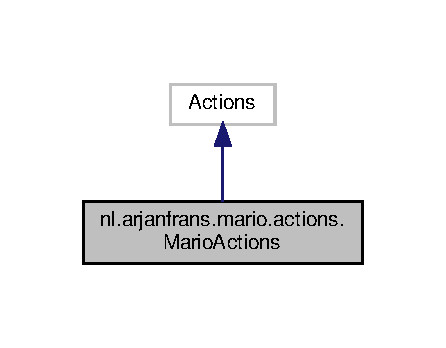
\includegraphics[width=214pt]{classnl_1_1arjanfrans_1_1mario_1_1actions_1_1MarioActions__inherit__graph}
\end{center}
\end{figure}


Collaboration diagram for nl.\+arjanfrans.\+mario.\+actions.\+Mario\+Actions\+:\nopagebreak
\begin{figure}[H]
\begin{center}
\leavevmode
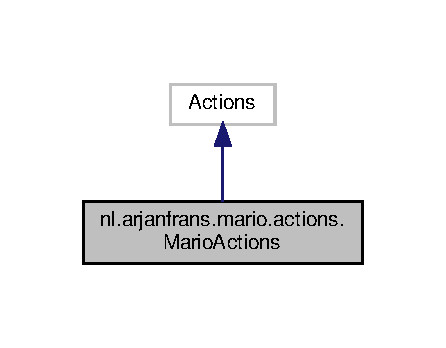
\includegraphics[width=214pt]{classnl_1_1arjanfrans_1_1mario_1_1actions_1_1MarioActions__coll__graph}
\end{center}
\end{figure}
\subsection*{Classes}
\begin{DoxyCompactItemize}
\item 
class {\bfseries big\+Mario}
\begin{DoxyCompactList}\small\item\em Inherited class Action. \end{DoxyCompactList}\item 
class {\bfseries finish\+Level}
\begin{DoxyCompactList}\small\item\em Inherited class Action. \end{DoxyCompactList}\item 
class {\bfseries flag\+Take\+Down}
\begin{DoxyCompactList}\small\item\em Inherited class Action. \end{DoxyCompactList}\item 
class {\bfseries set\+State}
\begin{DoxyCompactList}\small\item\em Inherited class Action. \end{DoxyCompactList}\item 
class {\bfseries stop\+Immume}
\begin{DoxyCompactList}\small\item\em Inherited class Action. \end{DoxyCompactList}\item 
class {\bfseries walk\+To}
\begin{DoxyCompactList}\small\item\em Inherited class Action. \end{DoxyCompactList}\end{DoxyCompactItemize}
\subsection*{Static Public Member Functions}
\begin{DoxyCompactItemize}
\item 
static Action \hyperlink{classnl_1_1arjanfrans_1_1mario_1_1actions_1_1MarioActions_ad04abb15058ffa3c3baf3a2301f4cf8c}{stop\+Immume\+Action} (\hyperlink{classnl_1_1arjanfrans_1_1mario_1_1model_1_1Mario}{Mario} actor)
\begin{DoxyCompactList}\small\item\em Stopping immune actions. \end{DoxyCompactList}\item 
static Action \hyperlink{classnl_1_1arjanfrans_1_1mario_1_1actions_1_1MarioActions_a0972a48677ce5de654513b88f8df56f1}{big\+Mario\+Action} (\hyperlink{classnl_1_1arjanfrans_1_1mario_1_1model_1_1Mario}{Mario} actor)
\begin{DoxyCompactList}\small\item\em Actions for big mario. \end{DoxyCompactList}\item 
static Action \hyperlink{classnl_1_1arjanfrans_1_1mario_1_1actions_1_1MarioActions_a4bfff41cf72d50a375c8546e05a0dfe9}{flag\+Take\+Down\+Action} (\hyperlink{classnl_1_1arjanfrans_1_1mario_1_1model_1_1Flag}{Flag} flag)
\begin{DoxyCompactList}\small\item\em Taking down the flag action. \end{DoxyCompactList}\item 
static Action \hyperlink{classnl_1_1arjanfrans_1_1mario_1_1actions_1_1MarioActions_a13ae9ce9afa4beb76cf7a74ec7167099}{finish\+Level\+Action} ()
\item 
static Action \hyperlink{classnl_1_1arjanfrans_1_1mario_1_1actions_1_1MarioActions_a908d016fe41950d737a578f8bb5e8122}{set\+State\+Action} (\hyperlink{classnl_1_1arjanfrans_1_1mario_1_1model_1_1Mario}{Mario} actor, State state)
\begin{DoxyCompactList}\small\item\em Set action state. \end{DoxyCompactList}\item 
static Action \hyperlink{classnl_1_1arjanfrans_1_1mario_1_1actions_1_1MarioActions_a68e2909268b910bb8568c9ca0730382f}{walk\+To\+Action} (\hyperlink{classnl_1_1arjanfrans_1_1mario_1_1model_1_1Mario}{Mario} actor, float x, float y)
\begin{DoxyCompactList}\small\item\em Action for walking to. \end{DoxyCompactList}\end{DoxyCompactItemize}


\subsection{Detailed Description}
Inherited class Actions. 

\subsection{Member Function Documentation}
\mbox{\Hypertarget{classnl_1_1arjanfrans_1_1mario_1_1actions_1_1MarioActions_a0972a48677ce5de654513b88f8df56f1}\label{classnl_1_1arjanfrans_1_1mario_1_1actions_1_1MarioActions_a0972a48677ce5de654513b88f8df56f1}} 
\index{nl\+::arjanfrans\+::mario\+::actions\+::\+Mario\+Actions@{nl\+::arjanfrans\+::mario\+::actions\+::\+Mario\+Actions}!big\+Mario\+Action@{big\+Mario\+Action}}
\index{big\+Mario\+Action@{big\+Mario\+Action}!nl\+::arjanfrans\+::mario\+::actions\+::\+Mario\+Actions@{nl\+::arjanfrans\+::mario\+::actions\+::\+Mario\+Actions}}
\subsubsection{\texorpdfstring{big\+Mario\+Action()}{bigMarioAction()}}
{\footnotesize\ttfamily static Action nl.\+arjanfrans.\+mario.\+actions.\+Mario\+Actions.\+big\+Mario\+Action (\begin{DoxyParamCaption}\item[{\hyperlink{classnl_1_1arjanfrans_1_1mario_1_1model_1_1Mario}{Mario}}]{actor }\end{DoxyParamCaption})\hspace{0.3cm}{\ttfamily [static]}}



Actions for big mario. 


\begin{DoxyParams}{Parameters}
{\em actor} & Mario object \\
\hline
\end{DoxyParams}
\begin{DoxyReturn}{Returns}
big\+Mario(actor) Action object 
\end{DoxyReturn}
\mbox{\Hypertarget{classnl_1_1arjanfrans_1_1mario_1_1actions_1_1MarioActions_a13ae9ce9afa4beb76cf7a74ec7167099}\label{classnl_1_1arjanfrans_1_1mario_1_1actions_1_1MarioActions_a13ae9ce9afa4beb76cf7a74ec7167099}} 
\index{nl\+::arjanfrans\+::mario\+::actions\+::\+Mario\+Actions@{nl\+::arjanfrans\+::mario\+::actions\+::\+Mario\+Actions}!finish\+Level\+Action@{finish\+Level\+Action}}
\index{finish\+Level\+Action@{finish\+Level\+Action}!nl\+::arjanfrans\+::mario\+::actions\+::\+Mario\+Actions@{nl\+::arjanfrans\+::mario\+::actions\+::\+Mario\+Actions}}
\subsubsection{\texorpdfstring{finish\+Level\+Action()}{finishLevelAction()}}
{\footnotesize\ttfamily static Action nl.\+arjanfrans.\+mario.\+actions.\+Mario\+Actions.\+finish\+Level\+Action (\begin{DoxyParamCaption}{ }\end{DoxyParamCaption})\hspace{0.3cm}{\ttfamily [static]}}

Set the World reset\+\_\+flag to true \begin{DoxyReturn}{Returns}
finish\+Level() Action object 
\end{DoxyReturn}
\mbox{\Hypertarget{classnl_1_1arjanfrans_1_1mario_1_1actions_1_1MarioActions_a4bfff41cf72d50a375c8546e05a0dfe9}\label{classnl_1_1arjanfrans_1_1mario_1_1actions_1_1MarioActions_a4bfff41cf72d50a375c8546e05a0dfe9}} 
\index{nl\+::arjanfrans\+::mario\+::actions\+::\+Mario\+Actions@{nl\+::arjanfrans\+::mario\+::actions\+::\+Mario\+Actions}!flag\+Take\+Down\+Action@{flag\+Take\+Down\+Action}}
\index{flag\+Take\+Down\+Action@{flag\+Take\+Down\+Action}!nl\+::arjanfrans\+::mario\+::actions\+::\+Mario\+Actions@{nl\+::arjanfrans\+::mario\+::actions\+::\+Mario\+Actions}}
\subsubsection{\texorpdfstring{flag\+Take\+Down\+Action()}{flagTakeDownAction()}}
{\footnotesize\ttfamily static Action nl.\+arjanfrans.\+mario.\+actions.\+Mario\+Actions.\+flag\+Take\+Down\+Action (\begin{DoxyParamCaption}\item[{\hyperlink{classnl_1_1arjanfrans_1_1mario_1_1model_1_1Flag}{Flag}}]{flag }\end{DoxyParamCaption})\hspace{0.3cm}{\ttfamily [static]}}



Taking down the flag action. 


\begin{DoxyParams}{Parameters}
{\em flag} & Flag object \\
\hline
\end{DoxyParams}
\begin{DoxyReturn}{Returns}
flag\+Take\+Down(flag) 
\end{DoxyReturn}
\mbox{\Hypertarget{classnl_1_1arjanfrans_1_1mario_1_1actions_1_1MarioActions_a908d016fe41950d737a578f8bb5e8122}\label{classnl_1_1arjanfrans_1_1mario_1_1actions_1_1MarioActions_a908d016fe41950d737a578f8bb5e8122}} 
\index{nl\+::arjanfrans\+::mario\+::actions\+::\+Mario\+Actions@{nl\+::arjanfrans\+::mario\+::actions\+::\+Mario\+Actions}!set\+State\+Action@{set\+State\+Action}}
\index{set\+State\+Action@{set\+State\+Action}!nl\+::arjanfrans\+::mario\+::actions\+::\+Mario\+Actions@{nl\+::arjanfrans\+::mario\+::actions\+::\+Mario\+Actions}}
\subsubsection{\texorpdfstring{set\+State\+Action()}{setStateAction()}}
{\footnotesize\ttfamily static Action nl.\+arjanfrans.\+mario.\+actions.\+Mario\+Actions.\+set\+State\+Action (\begin{DoxyParamCaption}\item[{\hyperlink{classnl_1_1arjanfrans_1_1mario_1_1model_1_1Mario}{Mario}}]{actor,  }\item[{State}]{state }\end{DoxyParamCaption})\hspace{0.3cm}{\ttfamily [static]}}



Set action state. 


\begin{DoxyParams}{Parameters}
{\em actor} & Mario object \\
\hline
{\em state} & State object \\
\hline
\end{DoxyParams}
\begin{DoxyReturn}{Returns}
set\+State(actor, state) Action object 
\end{DoxyReturn}
\mbox{\Hypertarget{classnl_1_1arjanfrans_1_1mario_1_1actions_1_1MarioActions_ad04abb15058ffa3c3baf3a2301f4cf8c}\label{classnl_1_1arjanfrans_1_1mario_1_1actions_1_1MarioActions_ad04abb15058ffa3c3baf3a2301f4cf8c}} 
\index{nl\+::arjanfrans\+::mario\+::actions\+::\+Mario\+Actions@{nl\+::arjanfrans\+::mario\+::actions\+::\+Mario\+Actions}!stop\+Immume\+Action@{stop\+Immume\+Action}}
\index{stop\+Immume\+Action@{stop\+Immume\+Action}!nl\+::arjanfrans\+::mario\+::actions\+::\+Mario\+Actions@{nl\+::arjanfrans\+::mario\+::actions\+::\+Mario\+Actions}}
\subsubsection{\texorpdfstring{stop\+Immume\+Action()}{stopImmumeAction()}}
{\footnotesize\ttfamily static Action nl.\+arjanfrans.\+mario.\+actions.\+Mario\+Actions.\+stop\+Immume\+Action (\begin{DoxyParamCaption}\item[{\hyperlink{classnl_1_1arjanfrans_1_1mario_1_1model_1_1Mario}{Mario}}]{actor }\end{DoxyParamCaption})\hspace{0.3cm}{\ttfamily [static]}}



Stopping immune actions. 


\begin{DoxyParams}{Parameters}
{\em actor} & Mario object \\
\hline
\end{DoxyParams}
\begin{DoxyReturn}{Returns}
true boolean value 
\end{DoxyReturn}
\mbox{\Hypertarget{classnl_1_1arjanfrans_1_1mario_1_1actions_1_1MarioActions_a68e2909268b910bb8568c9ca0730382f}\label{classnl_1_1arjanfrans_1_1mario_1_1actions_1_1MarioActions_a68e2909268b910bb8568c9ca0730382f}} 
\index{nl\+::arjanfrans\+::mario\+::actions\+::\+Mario\+Actions@{nl\+::arjanfrans\+::mario\+::actions\+::\+Mario\+Actions}!walk\+To\+Action@{walk\+To\+Action}}
\index{walk\+To\+Action@{walk\+To\+Action}!nl\+::arjanfrans\+::mario\+::actions\+::\+Mario\+Actions@{nl\+::arjanfrans\+::mario\+::actions\+::\+Mario\+Actions}}
\subsubsection{\texorpdfstring{walk\+To\+Action()}{walkToAction()}}
{\footnotesize\ttfamily static Action nl.\+arjanfrans.\+mario.\+actions.\+Mario\+Actions.\+walk\+To\+Action (\begin{DoxyParamCaption}\item[{\hyperlink{classnl_1_1arjanfrans_1_1mario_1_1model_1_1Mario}{Mario}}]{actor,  }\item[{float}]{x,  }\item[{float}]{y }\end{DoxyParamCaption})\hspace{0.3cm}{\ttfamily [static]}}



Action for walking to. 


\begin{DoxyParams}{Parameters}
{\em actor} & Mario object \\
\hline
{\em x} & coordinate \\
\hline
{\em y} & coordinate \\
\hline
\end{DoxyParams}


The documentation for this class was generated from the following file\+:\begin{DoxyCompactItemize}
\item 
core/src/nl/arjanfrans/mario/actions/\hyperlink{MarioActions_8java}{Mario\+Actions.\+java}\end{DoxyCompactItemize}

\hypertarget{classnl_1_1arjanfrans_1_1mario_1_1graphics_1_1MarioAnimation}{}\section{nl.\+arjanfrans.\+mario.\+graphics.\+Mario\+Animation Class Reference}
\label{classnl_1_1arjanfrans_1_1mario_1_1graphics_1_1MarioAnimation}\index{nl.\+arjanfrans.\+mario.\+graphics.\+Mario\+Animation@{nl.\+arjanfrans.\+mario.\+graphics.\+Mario\+Animation}}


This is a class that implements the abstract class, \hyperlink{classnl_1_1arjanfrans_1_1mario_1_1graphics_1_1CharacterAnimation}{Character\+Animation}, specifically for the animation of Mario.  




Inheritance diagram for nl.\+arjanfrans.\+mario.\+graphics.\+Mario\+Animation\+:
\nopagebreak
\begin{figure}[H]
\begin{center}
\leavevmode
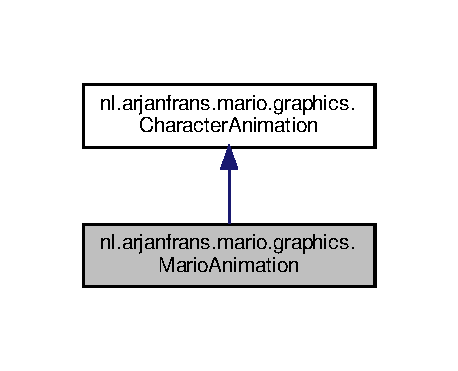
\includegraphics[width=220pt]{classnl_1_1arjanfrans_1_1mario_1_1graphics_1_1MarioAnimation__inherit__graph}
\end{center}
\end{figure}


Collaboration diagram for nl.\+arjanfrans.\+mario.\+graphics.\+Mario\+Animation\+:
\nopagebreak
\begin{figure}[H]
\begin{center}
\leavevmode
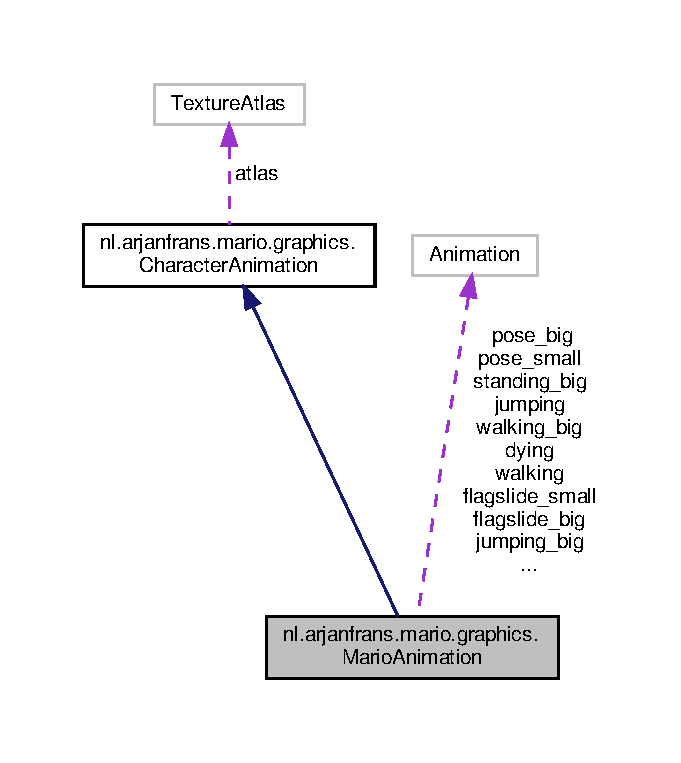
\includegraphics[width=327pt]{classnl_1_1arjanfrans_1_1mario_1_1graphics_1_1MarioAnimation__coll__graph}
\end{center}
\end{figure}
\subsection*{Public Member Functions}
\begin{DoxyCompactItemize}
\item 
\hyperlink{classnl_1_1arjanfrans_1_1mario_1_1graphics_1_1MarioAnimation_a15feb12f385241d47dfc71e2c90a8d06}{Mario\+Animation} ()
\begin{DoxyCompactList}\small\item\em Constructor method for \hyperlink{classnl_1_1arjanfrans_1_1mario_1_1graphics_1_1MarioAnimation}{Mario\+Animation}. \end{DoxyCompactList}\item 
Animation \hyperlink{classnl_1_1arjanfrans_1_1mario_1_1graphics_1_1MarioAnimation_a74455148020682d19d02372d17abd08f}{get\+Animation} (State state, int level)
\begin{DoxyCompactList}\small\item\em A method meant to retrieve a Mario animation based on the Mario\textquotesingle{}s state and size. \end{DoxyCompactList}\item 
Vector2 \hyperlink{classnl_1_1arjanfrans_1_1mario_1_1graphics_1_1MarioAnimation_aa4b74896a7eea77ece64354a3426b7c7}{get\+Dimensions} (State state, int level)
\begin{DoxyCompactList}\small\item\em A method meant to retrieve the dimensions of a Mario animation based on Mario\textquotesingle{}s state, and size. \end{DoxyCompactList}\item 
float \hyperlink{classnl_1_1arjanfrans_1_1mario_1_1graphics_1_1MarioAnimation_a8f05347b79edd167309067ed7d3c2794}{get\+Frame\+Width} (int level, float width)
\begin{DoxyCompactList}\small\item\em A method meant to retrieve the frame width of a Mario animation based on Mario\textquotesingle{}s size and width. \end{DoxyCompactList}\item 
float \hyperlink{classnl_1_1arjanfrans_1_1mario_1_1graphics_1_1MarioAnimation_ab0abed641099c07a993255f63b2f59b9}{get\+Frame\+Height} (int level, float height)
\begin{DoxyCompactList}\small\item\em A method meant to retrieve the frame height of a Mario animation based on Mario\textquotesingle{}s size and width. \end{DoxyCompactList}\end{DoxyCompactItemize}
\subsection*{Static Private Attributes}
\begin{DoxyCompactItemize}
\item 
\mbox{\Hypertarget{classnl_1_1arjanfrans_1_1mario_1_1graphics_1_1MarioAnimation_ab2d8a34ec8aa0c8c6c810e7f9f6b4ddf}\label{classnl_1_1arjanfrans_1_1mario_1_1graphics_1_1MarioAnimation_ab2d8a34ec8aa0c8c6c810e7f9f6b4ddf}} 
static Animation {\bfseries walking}
\item 
\mbox{\Hypertarget{classnl_1_1arjanfrans_1_1mario_1_1graphics_1_1MarioAnimation_a8e4e8383313a55a7c315a4a36c5593ef}\label{classnl_1_1arjanfrans_1_1mario_1_1graphics_1_1MarioAnimation_a8e4e8383313a55a7c315a4a36c5593ef}} 
static Animation {\bfseries standing}
\item 
\mbox{\Hypertarget{classnl_1_1arjanfrans_1_1mario_1_1graphics_1_1MarioAnimation_afb97c1ac80c5b193f5746ca0ba6652ac}\label{classnl_1_1arjanfrans_1_1mario_1_1graphics_1_1MarioAnimation_afb97c1ac80c5b193f5746ca0ba6652ac}} 
static Animation {\bfseries jumping}
\item 
\mbox{\Hypertarget{classnl_1_1arjanfrans_1_1mario_1_1graphics_1_1MarioAnimation_a84cdceb1d47fc66545593a28a95eb9b5}\label{classnl_1_1arjanfrans_1_1mario_1_1graphics_1_1MarioAnimation_a84cdceb1d47fc66545593a28a95eb9b5}} 
static Animation {\bfseries dying}
\item 
\mbox{\Hypertarget{classnl_1_1arjanfrans_1_1mario_1_1graphics_1_1MarioAnimation_aa22378aa25f438d40b22ee75514feb83}\label{classnl_1_1arjanfrans_1_1mario_1_1graphics_1_1MarioAnimation_aa22378aa25f438d40b22ee75514feb83}} 
static Animation {\bfseries walking\+\_\+big}
\item 
\mbox{\Hypertarget{classnl_1_1arjanfrans_1_1mario_1_1graphics_1_1MarioAnimation_ac2254395ad715b136a7313968da53333}\label{classnl_1_1arjanfrans_1_1mario_1_1graphics_1_1MarioAnimation_ac2254395ad715b136a7313968da53333}} 
static Animation {\bfseries standing\+\_\+big}
\item 
\mbox{\Hypertarget{classnl_1_1arjanfrans_1_1mario_1_1graphics_1_1MarioAnimation_aaacf6455b26bf4f362e31b903c3f0e37}\label{classnl_1_1arjanfrans_1_1mario_1_1graphics_1_1MarioAnimation_aaacf6455b26bf4f362e31b903c3f0e37}} 
static Animation {\bfseries jumping\+\_\+big}
\item 
\mbox{\Hypertarget{classnl_1_1arjanfrans_1_1mario_1_1graphics_1_1MarioAnimation_af1a95c0234d63b8775d9924d875ca988}\label{classnl_1_1arjanfrans_1_1mario_1_1graphics_1_1MarioAnimation_af1a95c0234d63b8775d9924d875ca988}} 
static Animation {\bfseries crouch\+\_\+big}
\item 
\mbox{\Hypertarget{classnl_1_1arjanfrans_1_1mario_1_1graphics_1_1MarioAnimation_aa06a8c57d4612d85fb944cedca8c9298}\label{classnl_1_1arjanfrans_1_1mario_1_1graphics_1_1MarioAnimation_aa06a8c57d4612d85fb944cedca8c9298}} 
static Animation {\bfseries flagslide\+\_\+small}
\item 
\mbox{\Hypertarget{classnl_1_1arjanfrans_1_1mario_1_1graphics_1_1MarioAnimation_a155d95a2c30ff796fda2a9e418d7c19b}\label{classnl_1_1arjanfrans_1_1mario_1_1graphics_1_1MarioAnimation_a155d95a2c30ff796fda2a9e418d7c19b}} 
static Animation {\bfseries flagslide\+\_\+big}
\item 
\mbox{\Hypertarget{classnl_1_1arjanfrans_1_1mario_1_1graphics_1_1MarioAnimation_a03ad11c621a17cfffaad8f0973bece7e}\label{classnl_1_1arjanfrans_1_1mario_1_1graphics_1_1MarioAnimation_a03ad11c621a17cfffaad8f0973bece7e}} 
static Animation {\bfseries pose\+\_\+small}
\item 
\mbox{\Hypertarget{classnl_1_1arjanfrans_1_1mario_1_1graphics_1_1MarioAnimation_a2add793b8c9cae8344f6f63b63a02724}\label{classnl_1_1arjanfrans_1_1mario_1_1graphics_1_1MarioAnimation_a2add793b8c9cae8344f6f63b63a02724}} 
static Animation {\bfseries pose\+\_\+big}
\end{DoxyCompactItemize}
\subsection*{Additional Inherited Members}


\subsection{Detailed Description}
This is a class that implements the abstract class, \hyperlink{classnl_1_1arjanfrans_1_1mario_1_1graphics_1_1CharacterAnimation}{Character\+Animation}, specifically for the animation of Mario. 

\subsection{Constructor \& Destructor Documentation}
\mbox{\Hypertarget{classnl_1_1arjanfrans_1_1mario_1_1graphics_1_1MarioAnimation_a15feb12f385241d47dfc71e2c90a8d06}\label{classnl_1_1arjanfrans_1_1mario_1_1graphics_1_1MarioAnimation_a15feb12f385241d47dfc71e2c90a8d06}} 
\index{nl\+::arjanfrans\+::mario\+::graphics\+::\+Mario\+Animation@{nl\+::arjanfrans\+::mario\+::graphics\+::\+Mario\+Animation}!Mario\+Animation@{Mario\+Animation}}
\index{Mario\+Animation@{Mario\+Animation}!nl\+::arjanfrans\+::mario\+::graphics\+::\+Mario\+Animation@{nl\+::arjanfrans\+::mario\+::graphics\+::\+Mario\+Animation}}
\subsubsection{\texorpdfstring{Mario\+Animation()}{MarioAnimation()}}
{\footnotesize\ttfamily nl.\+arjanfrans.\+mario.\+graphics.\+Mario\+Animation.\+Mario\+Animation (\begin{DoxyParamCaption}{ }\end{DoxyParamCaption})}



Constructor method for \hyperlink{classnl_1_1arjanfrans_1_1mario_1_1graphics_1_1MarioAnimation}{Mario\+Animation}. 

Method which initializes an instance of \hyperlink{classnl_1_1arjanfrans_1_1mario_1_1graphics_1_1MarioAnimation}{Mario\+Animation}. \begin{DoxyReturn}{Returns}
An instance of \hyperlink{classnl_1_1arjanfrans_1_1mario_1_1graphics_1_1MarioAnimation}{Mario\+Animation} 
\end{DoxyReturn}


\subsection{Member Function Documentation}
\mbox{\Hypertarget{classnl_1_1arjanfrans_1_1mario_1_1graphics_1_1MarioAnimation_a74455148020682d19d02372d17abd08f}\label{classnl_1_1arjanfrans_1_1mario_1_1graphics_1_1MarioAnimation_a74455148020682d19d02372d17abd08f}} 
\index{nl\+::arjanfrans\+::mario\+::graphics\+::\+Mario\+Animation@{nl\+::arjanfrans\+::mario\+::graphics\+::\+Mario\+Animation}!get\+Animation@{get\+Animation}}
\index{get\+Animation@{get\+Animation}!nl\+::arjanfrans\+::mario\+::graphics\+::\+Mario\+Animation@{nl\+::arjanfrans\+::mario\+::graphics\+::\+Mario\+Animation}}
\subsubsection{\texorpdfstring{get\+Animation()}{getAnimation()}}
{\footnotesize\ttfamily Animation nl.\+arjanfrans.\+mario.\+graphics.\+Mario\+Animation.\+get\+Animation (\begin{DoxyParamCaption}\item[{State}]{state,  }\item[{int}]{level }\end{DoxyParamCaption})}



A method meant to retrieve a Mario animation based on the Mario\textquotesingle{}s state and size. 


\begin{DoxyParams}{Parameters}
{\em state} & -\/ the state of the Goomba, refers to the State enum class. \\
\hline
{\em level} & -\/ an integer indicating Mario\textquotesingle{}s current size. \\
\hline
\end{DoxyParams}
\begin{DoxyReturn}{Returns}
An instance of Animation 
\end{DoxyReturn}
\mbox{\Hypertarget{classnl_1_1arjanfrans_1_1mario_1_1graphics_1_1MarioAnimation_aa4b74896a7eea77ece64354a3426b7c7}\label{classnl_1_1arjanfrans_1_1mario_1_1graphics_1_1MarioAnimation_aa4b74896a7eea77ece64354a3426b7c7}} 
\index{nl\+::arjanfrans\+::mario\+::graphics\+::\+Mario\+Animation@{nl\+::arjanfrans\+::mario\+::graphics\+::\+Mario\+Animation}!get\+Dimensions@{get\+Dimensions}}
\index{get\+Dimensions@{get\+Dimensions}!nl\+::arjanfrans\+::mario\+::graphics\+::\+Mario\+Animation@{nl\+::arjanfrans\+::mario\+::graphics\+::\+Mario\+Animation}}
\subsubsection{\texorpdfstring{get\+Dimensions()}{getDimensions()}}
{\footnotesize\ttfamily Vector2 nl.\+arjanfrans.\+mario.\+graphics.\+Mario\+Animation.\+get\+Dimensions (\begin{DoxyParamCaption}\item[{State}]{state,  }\item[{int}]{level }\end{DoxyParamCaption})}



A method meant to retrieve the dimensions of a Mario animation based on Mario\textquotesingle{}s state, and size. 


\begin{DoxyParams}{Parameters}
{\em state} & -\/ the state of the Goomba, refers to the State enum class. \\
\hline
{\em level} & -\/ an integer indicating Mario\textquotesingle{}s current size. \\
\hline
\end{DoxyParams}
\begin{DoxyReturn}{Returns}
An instance of Vector2. 
\end{DoxyReturn}
\mbox{\Hypertarget{classnl_1_1arjanfrans_1_1mario_1_1graphics_1_1MarioAnimation_ab0abed641099c07a993255f63b2f59b9}\label{classnl_1_1arjanfrans_1_1mario_1_1graphics_1_1MarioAnimation_ab0abed641099c07a993255f63b2f59b9}} 
\index{nl\+::arjanfrans\+::mario\+::graphics\+::\+Mario\+Animation@{nl\+::arjanfrans\+::mario\+::graphics\+::\+Mario\+Animation}!get\+Frame\+Height@{get\+Frame\+Height}}
\index{get\+Frame\+Height@{get\+Frame\+Height}!nl\+::arjanfrans\+::mario\+::graphics\+::\+Mario\+Animation@{nl\+::arjanfrans\+::mario\+::graphics\+::\+Mario\+Animation}}
\subsubsection{\texorpdfstring{get\+Frame\+Height()}{getFrameHeight()}}
{\footnotesize\ttfamily float nl.\+arjanfrans.\+mario.\+graphics.\+Mario\+Animation.\+get\+Frame\+Height (\begin{DoxyParamCaption}\item[{int}]{level,  }\item[{float}]{height }\end{DoxyParamCaption})}



A method meant to retrieve the frame height of a Mario animation based on Mario\textquotesingle{}s size and width. 


\begin{DoxyParams}{Parameters}
{\em height} & -\/ a float representing the height of the frame. \\
\hline
{\em level} & -\/ an integer indicating Mario\textquotesingle{}s current size. \\
\hline
\end{DoxyParams}
\begin{DoxyReturn}{Returns}
a float representing the frame height. 
\end{DoxyReturn}
\mbox{\Hypertarget{classnl_1_1arjanfrans_1_1mario_1_1graphics_1_1MarioAnimation_a8f05347b79edd167309067ed7d3c2794}\label{classnl_1_1arjanfrans_1_1mario_1_1graphics_1_1MarioAnimation_a8f05347b79edd167309067ed7d3c2794}} 
\index{nl\+::arjanfrans\+::mario\+::graphics\+::\+Mario\+Animation@{nl\+::arjanfrans\+::mario\+::graphics\+::\+Mario\+Animation}!get\+Frame\+Width@{get\+Frame\+Width}}
\index{get\+Frame\+Width@{get\+Frame\+Width}!nl\+::arjanfrans\+::mario\+::graphics\+::\+Mario\+Animation@{nl\+::arjanfrans\+::mario\+::graphics\+::\+Mario\+Animation}}
\subsubsection{\texorpdfstring{get\+Frame\+Width()}{getFrameWidth()}}
{\footnotesize\ttfamily float nl.\+arjanfrans.\+mario.\+graphics.\+Mario\+Animation.\+get\+Frame\+Width (\begin{DoxyParamCaption}\item[{int}]{level,  }\item[{float}]{width }\end{DoxyParamCaption})}



A method meant to retrieve the frame width of a Mario animation based on Mario\textquotesingle{}s size and width. 


\begin{DoxyParams}{Parameters}
{\em width} & -\/ a float representing the width of the frame. \\
\hline
{\em level} & -\/ an integer indicating Mario\textquotesingle{}s current size. \\
\hline
\end{DoxyParams}
\begin{DoxyReturn}{Returns}
a float representing the frame witdh. 
\end{DoxyReturn}


The documentation for this class was generated from the following file\+:\begin{DoxyCompactItemize}
\item 
core/src/nl/arjanfrans/mario/graphics/Mario\+Animation.\+java\end{DoxyCompactItemize}

\hypertarget{classnl_1_1arjanfrans_1_1mario_1_1MarioGame}{}\section{nl.\+arjanfrans.\+mario.\+Mario\+Game Class Reference}
\label{classnl_1_1arjanfrans_1_1mario_1_1MarioGame}\index{nl.\+arjanfrans.\+mario.\+Mario\+Game@{nl.\+arjanfrans.\+mario.\+Mario\+Game}}


The class meant to render the game.  




Inheritance diagram for nl.\+arjanfrans.\+mario.\+Mario\+Game\+:\nopagebreak
\begin{figure}[H]
\begin{center}
\leavevmode
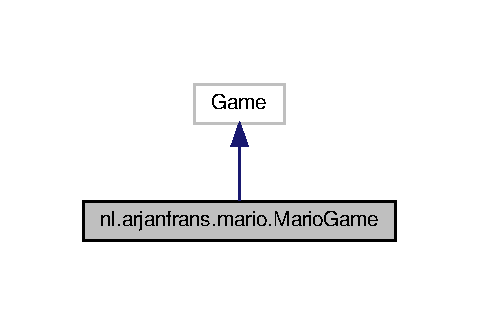
\includegraphics[width=230pt]{classnl_1_1arjanfrans_1_1mario_1_1MarioGame__inherit__graph}
\end{center}
\end{figure}


Collaboration diagram for nl.\+arjanfrans.\+mario.\+Mario\+Game\+:
\nopagebreak
\begin{figure}[H]
\begin{center}
\leavevmode
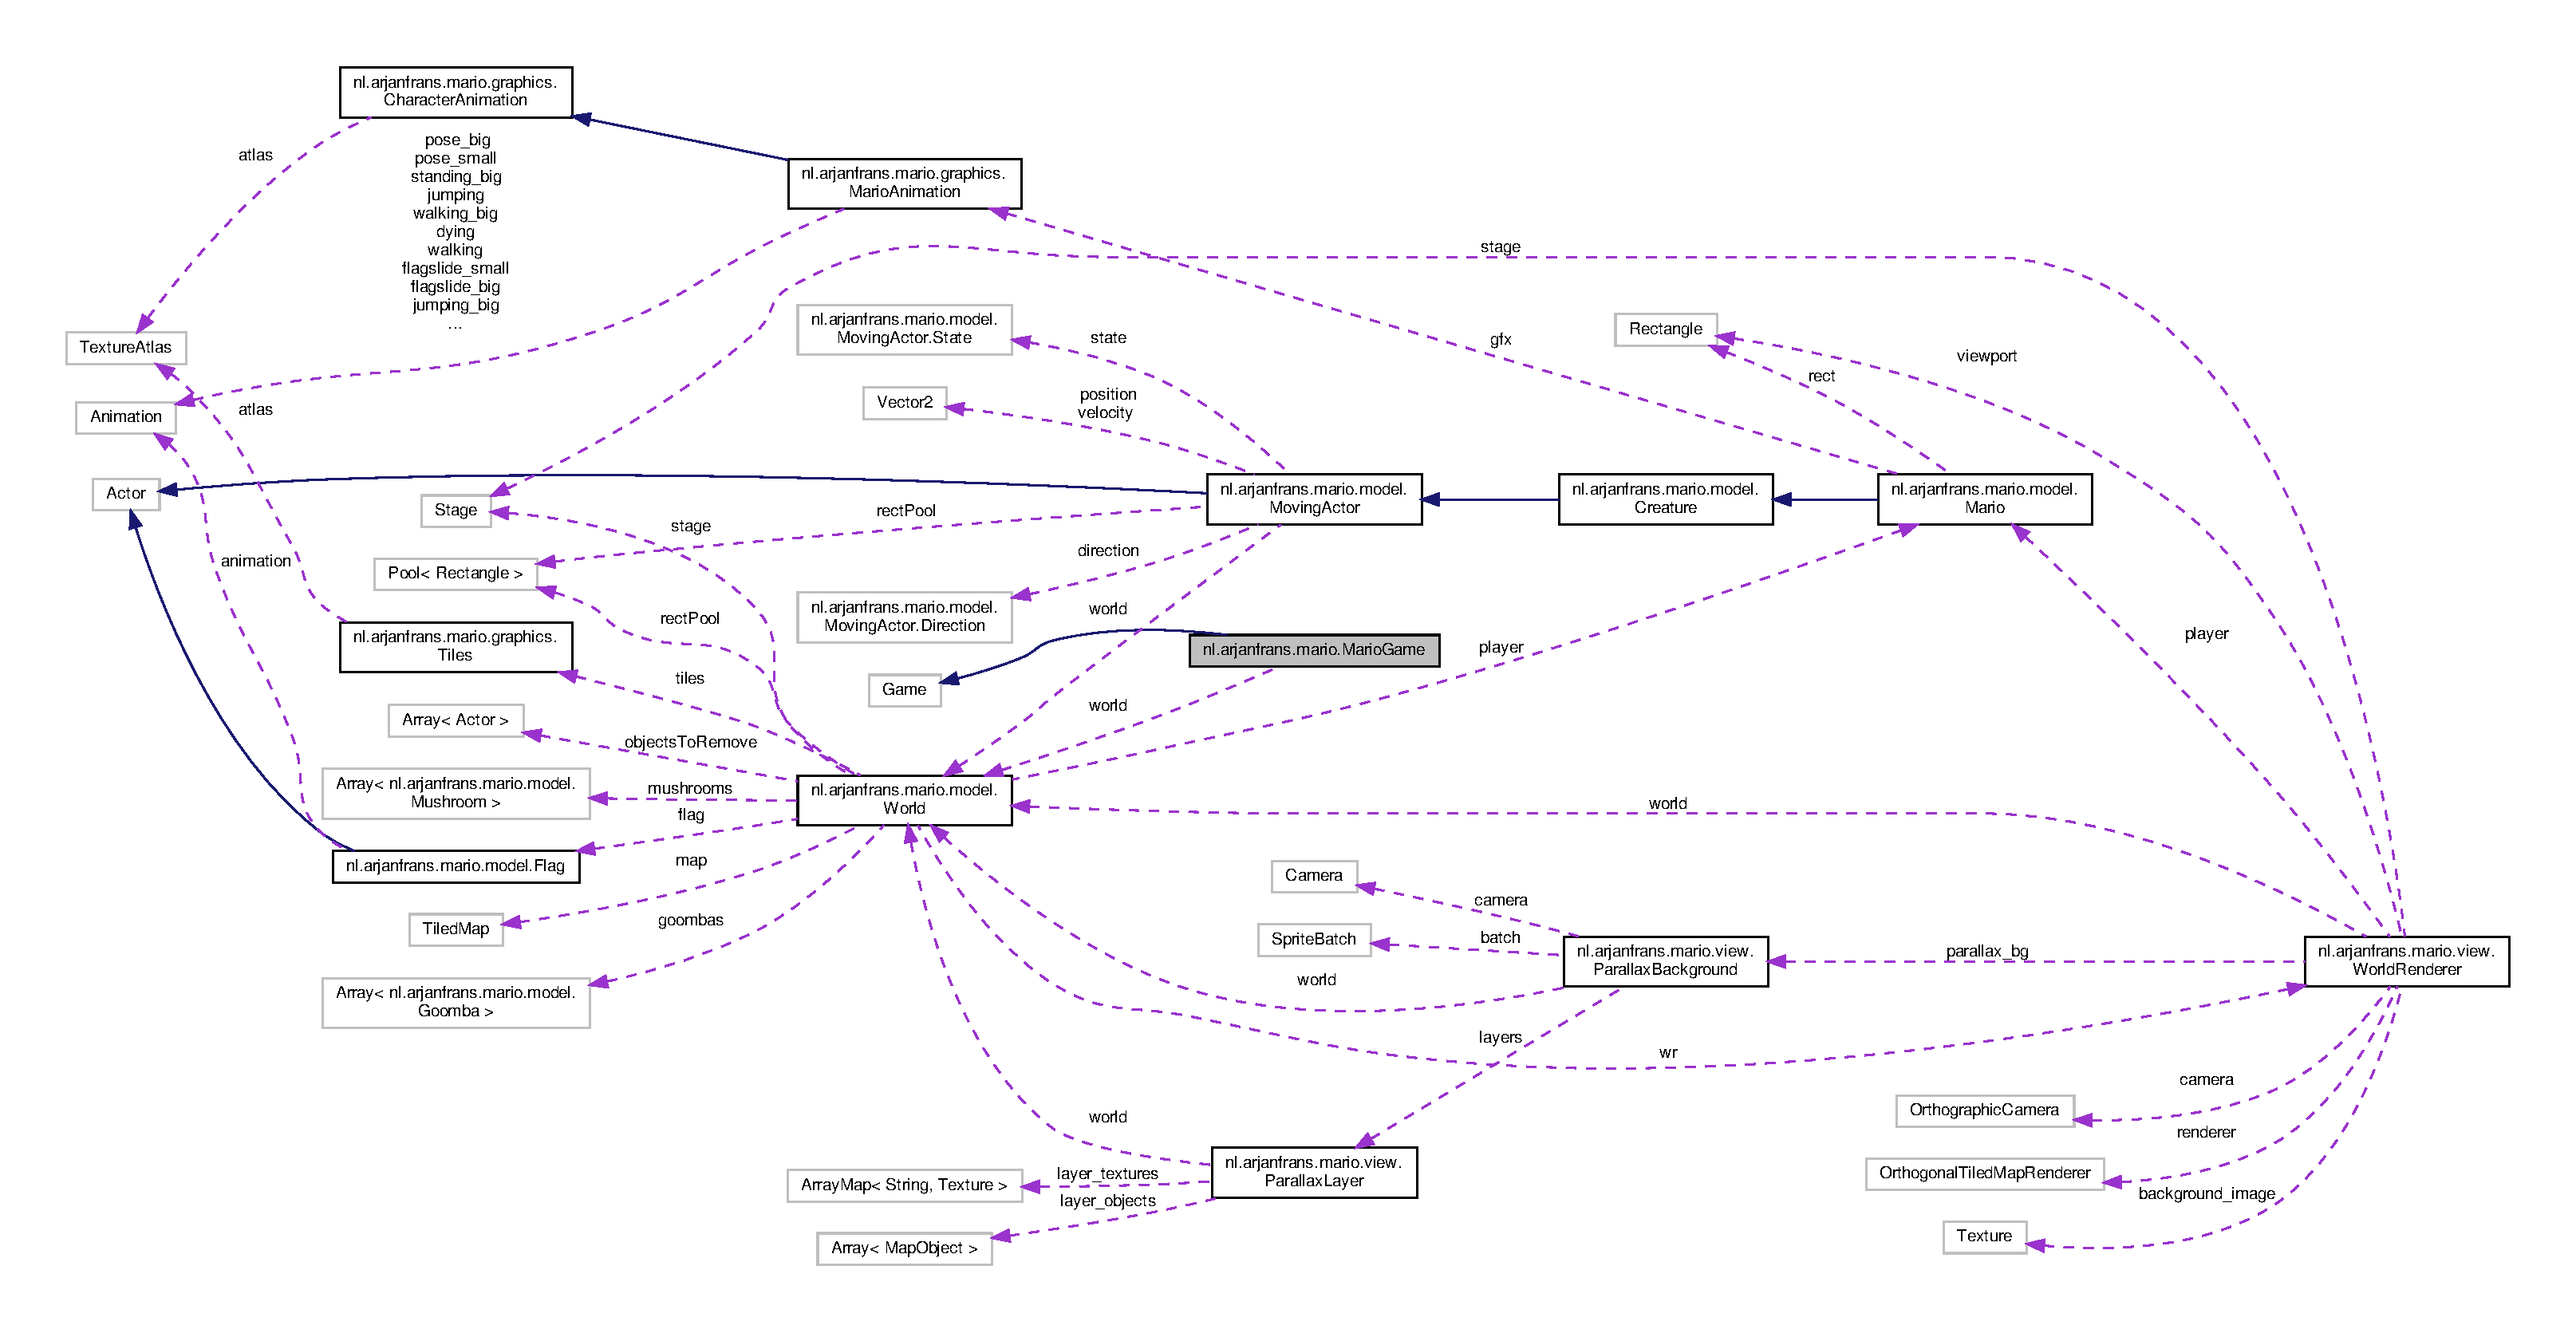
\includegraphics[width=350pt]{classnl_1_1arjanfrans_1_1mario_1_1MarioGame__coll__graph}
\end{center}
\end{figure}
\subsection*{Public Member Functions}
\begin{DoxyCompactItemize}
\item 
\mbox{\Hypertarget{classnl_1_1arjanfrans_1_1mario_1_1MarioGame_aef8d04f801a81a7948105c486e5e6b1b}\label{classnl_1_1arjanfrans_1_1mario_1_1MarioGame_aef8d04f801a81a7948105c486e5e6b1b}} 
void \hyperlink{classnl_1_1arjanfrans_1_1mario_1_1MarioGame_aef8d04f801a81a7948105c486e5e6b1b}{create} ()
\begin{DoxyCompactList}\small\item\em The method creates a new World object. \end{DoxyCompactList}\item 
\mbox{\Hypertarget{classnl_1_1arjanfrans_1_1mario_1_1MarioGame_a6aa0140a701c4f9cb620204cf319e826}\label{classnl_1_1arjanfrans_1_1mario_1_1MarioGame_a6aa0140a701c4f9cb620204cf319e826}} 
void \hyperlink{classnl_1_1arjanfrans_1_1mario_1_1MarioGame_a6aa0140a701c4f9cb620204cf319e826}{dispose} ()
\begin{DoxyCompactList}\small\item\em The method disposes of a World object. \end{DoxyCompactList}\item 
\mbox{\Hypertarget{classnl_1_1arjanfrans_1_1mario_1_1MarioGame_aa398b3da01339cdb1981b32c4bbed52b}\label{classnl_1_1arjanfrans_1_1mario_1_1MarioGame_aa398b3da01339cdb1981b32c4bbed52b}} 
void \hyperlink{classnl_1_1arjanfrans_1_1mario_1_1MarioGame_aa398b3da01339cdb1981b32c4bbed52b}{resize} (int width, int height)
\begin{DoxyCompactList}\small\item\em The method resizes the game, as the window is resized. \end{DoxyCompactList}\item 
\mbox{\Hypertarget{classnl_1_1arjanfrans_1_1mario_1_1MarioGame_af3a9dd63e2fba4bedc74e25cd4fec05c}\label{classnl_1_1arjanfrans_1_1mario_1_1MarioGame_af3a9dd63e2fba4bedc74e25cd4fec05c}} 
void {\bfseries pause} ()
\item 
\mbox{\Hypertarget{classnl_1_1arjanfrans_1_1mario_1_1MarioGame_a31b58f0d118a0f087c8a616157354480}\label{classnl_1_1arjanfrans_1_1mario_1_1MarioGame_a31b58f0d118a0f087c8a616157354480}} 
void {\bfseries resume} ()
\item 
\mbox{\Hypertarget{classnl_1_1arjanfrans_1_1mario_1_1MarioGame_a169a3a638096d8929297d095051cbc6c}\label{classnl_1_1arjanfrans_1_1mario_1_1MarioGame_a169a3a638096d8929297d095051cbc6c}} 
void \hyperlink{classnl_1_1arjanfrans_1_1mario_1_1MarioGame_a169a3a638096d8929297d095051cbc6c}{render} ()
\begin{DoxyCompactList}\small\item\em The method makes any necessary updates to the game, and calls when the application should render itself. \end{DoxyCompactList}\end{DoxyCompactItemize}
\subsection*{Static Public Attributes}
\begin{DoxyCompactItemize}
\item 
\mbox{\Hypertarget{classnl_1_1arjanfrans_1_1mario_1_1MarioGame_a0b84320779d5ffb3cea028477669a27a}\label{classnl_1_1arjanfrans_1_1mario_1_1MarioGame_a0b84320779d5ffb3cea028477669a27a}} 
static final String {\bfseries V\+E\+R\+S\+I\+ON} = \char`\"{}0.\+01\char`\"{}
\item 
\mbox{\Hypertarget{classnl_1_1arjanfrans_1_1mario_1_1MarioGame_a8384a6d9e3db1e7aef33e9ffe3b3fd29}\label{classnl_1_1arjanfrans_1_1mario_1_1MarioGame_a8384a6d9e3db1e7aef33e9ffe3b3fd29}} 
static final boolean {\bfseries D\+E\+B\+UG} = true
\item 
\mbox{\Hypertarget{classnl_1_1arjanfrans_1_1mario_1_1MarioGame_ac475b747d4a93178a0ddccd757ab5099}\label{classnl_1_1arjanfrans_1_1mario_1_1MarioGame_ac475b747d4a93178a0ddccd757ab5099}} 
static final int {\bfseries F\+PS} = 60
\end{DoxyCompactItemize}
\subsection*{Private Attributes}
\begin{DoxyCompactItemize}
\item 
\mbox{\Hypertarget{classnl_1_1arjanfrans_1_1mario_1_1MarioGame_ac9b0b84fd35672fdc4b6c3fdfb7ac65c}\label{classnl_1_1arjanfrans_1_1mario_1_1MarioGame_ac9b0b84fd35672fdc4b6c3fdfb7ac65c}} 
\hyperlink{classnl_1_1arjanfrans_1_1mario_1_1model_1_1World}{World} {\bfseries world}
\end{DoxyCompactItemize}


\subsection{Detailed Description}
The class meant to render the game. 

The documentation for this class was generated from the following file\+:\begin{DoxyCompactItemize}
\item 
core/src/nl/arjanfrans/mario/Mario\+Game.\+java\end{DoxyCompactItemize}

\hypertarget{classnl_1_1arjanfrans_1_1mario_1_1input_1_1MarioInput}{}\section{nl.\+arjanfrans.\+mario.\+input.\+Mario\+Input Class Reference}
\label{classnl_1_1arjanfrans_1_1mario_1_1input_1_1MarioInput}\index{nl.\+arjanfrans.\+mario.\+input.\+Mario\+Input@{nl.\+arjanfrans.\+mario.\+input.\+Mario\+Input}}


Inherited class that overrides mario input methods.  




Inheritance diagram for nl.\+arjanfrans.\+mario.\+input.\+Mario\+Input\+:\nopagebreak
\begin{figure}[H]
\begin{center}
\leavevmode
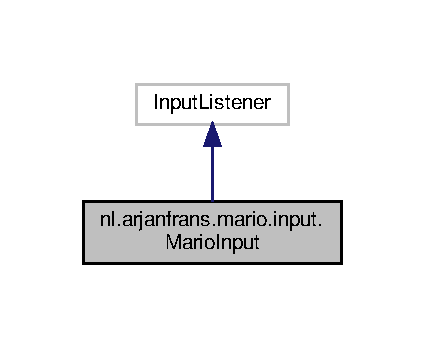
\includegraphics[width=204pt]{classnl_1_1arjanfrans_1_1mario_1_1input_1_1MarioInput__inherit__graph}
\end{center}
\end{figure}


Collaboration diagram for nl.\+arjanfrans.\+mario.\+input.\+Mario\+Input\+:\nopagebreak
\begin{figure}[H]
\begin{center}
\leavevmode
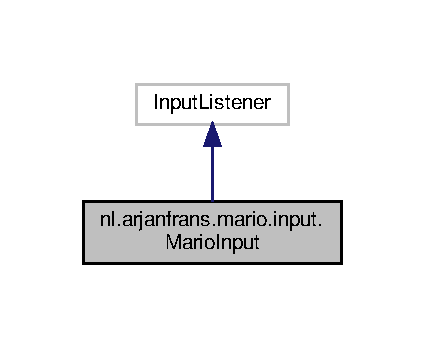
\includegraphics[width=204pt]{classnl_1_1arjanfrans_1_1mario_1_1input_1_1MarioInput__coll__graph}
\end{center}
\end{figure}
\subsection*{Public Member Functions}
\begin{DoxyCompactItemize}
\item 
boolean \hyperlink{classnl_1_1arjanfrans_1_1mario_1_1input_1_1MarioInput_ab9bcfe25e4249c77c623a9491a6f4e9e}{touch\+Down} (Input\+Event event, float x, float y, int pointer, int button)
\item 
void \hyperlink{classnl_1_1arjanfrans_1_1mario_1_1input_1_1MarioInput_a24f8afd60f2973ca334f1291fca84f35}{touch\+Up} (Input\+Event event, float x, float y, int pointer, int button)
\item 
boolean \hyperlink{classnl_1_1arjanfrans_1_1mario_1_1input_1_1MarioInput_a83589758280a9bd9ed25f6265052843c}{key\+Down} (Input\+Event event, int keycode)
\item 
boolean \hyperlink{classnl_1_1arjanfrans_1_1mario_1_1input_1_1MarioInput_aafe388c2a8940c27a508ca2c7b1599cb}{key\+Up} (Input\+Event event, int keycode)
\end{DoxyCompactItemize}


\subsection{Detailed Description}
Inherited class that overrides mario input methods. 

\subsection{Member Function Documentation}
\mbox{\Hypertarget{classnl_1_1arjanfrans_1_1mario_1_1input_1_1MarioInput_a83589758280a9bd9ed25f6265052843c}\label{classnl_1_1arjanfrans_1_1mario_1_1input_1_1MarioInput_a83589758280a9bd9ed25f6265052843c}} 
\index{nl\+::arjanfrans\+::mario\+::input\+::\+Mario\+Input@{nl\+::arjanfrans\+::mario\+::input\+::\+Mario\+Input}!key\+Down@{key\+Down}}
\index{key\+Down@{key\+Down}!nl\+::arjanfrans\+::mario\+::input\+::\+Mario\+Input@{nl\+::arjanfrans\+::mario\+::input\+::\+Mario\+Input}}
\subsubsection{\texorpdfstring{key\+Down()}{keyDown()}}
{\footnotesize\ttfamily boolean nl.\+arjanfrans.\+mario.\+input.\+Mario\+Input.\+key\+Down (\begin{DoxyParamCaption}\item[{Input\+Event}]{event,  }\item[{int}]{keycode }\end{DoxyParamCaption})}





\mbox{\Hypertarget{classnl_1_1arjanfrans_1_1mario_1_1input_1_1MarioInput_aafe388c2a8940c27a508ca2c7b1599cb}\label{classnl_1_1arjanfrans_1_1mario_1_1input_1_1MarioInput_aafe388c2a8940c27a508ca2c7b1599cb}} 
\index{nl\+::arjanfrans\+::mario\+::input\+::\+Mario\+Input@{nl\+::arjanfrans\+::mario\+::input\+::\+Mario\+Input}!key\+Up@{key\+Up}}
\index{key\+Up@{key\+Up}!nl\+::arjanfrans\+::mario\+::input\+::\+Mario\+Input@{nl\+::arjanfrans\+::mario\+::input\+::\+Mario\+Input}}
\subsubsection{\texorpdfstring{key\+Up()}{keyUp()}}
{\footnotesize\ttfamily boolean nl.\+arjanfrans.\+mario.\+input.\+Mario\+Input.\+key\+Up (\begin{DoxyParamCaption}\item[{Input\+Event}]{event,  }\item[{int}]{keycode }\end{DoxyParamCaption})}





\mbox{\Hypertarget{classnl_1_1arjanfrans_1_1mario_1_1input_1_1MarioInput_ab9bcfe25e4249c77c623a9491a6f4e9e}\label{classnl_1_1arjanfrans_1_1mario_1_1input_1_1MarioInput_ab9bcfe25e4249c77c623a9491a6f4e9e}} 
\index{nl\+::arjanfrans\+::mario\+::input\+::\+Mario\+Input@{nl\+::arjanfrans\+::mario\+::input\+::\+Mario\+Input}!touch\+Down@{touch\+Down}}
\index{touch\+Down@{touch\+Down}!nl\+::arjanfrans\+::mario\+::input\+::\+Mario\+Input@{nl\+::arjanfrans\+::mario\+::input\+::\+Mario\+Input}}
\subsubsection{\texorpdfstring{touch\+Down()}{touchDown()}}
{\footnotesize\ttfamily boolean nl.\+arjanfrans.\+mario.\+input.\+Mario\+Input.\+touch\+Down (\begin{DoxyParamCaption}\item[{Input\+Event}]{event,  }\item[{float}]{x,  }\item[{float}]{y,  }\item[{int}]{pointer,  }\item[{int}]{button }\end{DoxyParamCaption})}





\mbox{\Hypertarget{classnl_1_1arjanfrans_1_1mario_1_1input_1_1MarioInput_a24f8afd60f2973ca334f1291fca84f35}\label{classnl_1_1arjanfrans_1_1mario_1_1input_1_1MarioInput_a24f8afd60f2973ca334f1291fca84f35}} 
\index{nl\+::arjanfrans\+::mario\+::input\+::\+Mario\+Input@{nl\+::arjanfrans\+::mario\+::input\+::\+Mario\+Input}!touch\+Up@{touch\+Up}}
\index{touch\+Up@{touch\+Up}!nl\+::arjanfrans\+::mario\+::input\+::\+Mario\+Input@{nl\+::arjanfrans\+::mario\+::input\+::\+Mario\+Input}}
\subsubsection{\texorpdfstring{touch\+Up()}{touchUp()}}
{\footnotesize\ttfamily void nl.\+arjanfrans.\+mario.\+input.\+Mario\+Input.\+touch\+Up (\begin{DoxyParamCaption}\item[{Input\+Event}]{event,  }\item[{float}]{x,  }\item[{float}]{y,  }\item[{int}]{pointer,  }\item[{int}]{button }\end{DoxyParamCaption})}







The documentation for this class was generated from the following file\+:\begin{DoxyCompactItemize}
\item 
core/src/nl/arjanfrans/mario/input/\hyperlink{MarioInput_8java}{Mario\+Input.\+java}\end{DoxyCompactItemize}

\hypertarget{classnl_1_1arjanfrans_1_1mario_1_1actions_1_1MoveableActions}{}\section{nl.\+arjanfrans.\+mario.\+actions.\+Moveable\+Actions Class Reference}
\label{classnl_1_1arjanfrans_1_1mario_1_1actions_1_1MoveableActions}\index{nl.\+arjanfrans.\+mario.\+actions.\+Moveable\+Actions@{nl.\+arjanfrans.\+mario.\+actions.\+Moveable\+Actions}}


Inherited class Actions.  




Inheritance diagram for nl.\+arjanfrans.\+mario.\+actions.\+Moveable\+Actions\+:\nopagebreak
\begin{figure}[H]
\begin{center}
\leavevmode
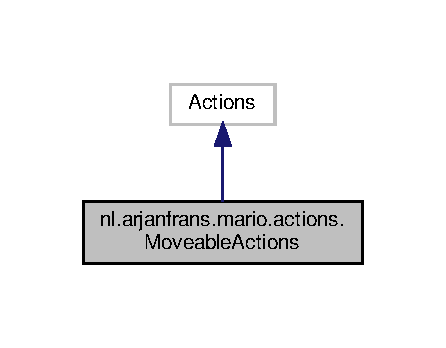
\includegraphics[width=214pt]{classnl_1_1arjanfrans_1_1mario_1_1actions_1_1MoveableActions__inherit__graph}
\end{center}
\end{figure}


Collaboration diagram for nl.\+arjanfrans.\+mario.\+actions.\+Moveable\+Actions\+:\nopagebreak
\begin{figure}[H]
\begin{center}
\leavevmode
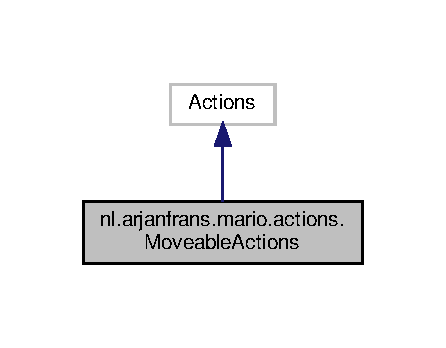
\includegraphics[width=214pt]{classnl_1_1arjanfrans_1_1mario_1_1actions_1_1MoveableActions__coll__graph}
\end{center}
\end{figure}
\subsection*{Classes}
\begin{DoxyCompactItemize}
\item 
class {\bfseries Die}
\begin{DoxyCompactList}\small\item\em Inherited class Action. \end{DoxyCompactList}\item 
class {\bfseries start\+Moving}
\begin{DoxyCompactList}\small\item\em Inherited class Action. \end{DoxyCompactList}\end{DoxyCompactItemize}
\subsection*{Static Public Member Functions}
\begin{DoxyCompactItemize}
\item 
static Action \hyperlink{classnl_1_1arjanfrans_1_1mario_1_1actions_1_1MoveableActions_a470d03df0851eeaea55886b46dc82c90}{Die\+Action} (Actor actor)
\begin{DoxyCompactList}\small\item\em Action for Mario\textquotesingle{}s death. \end{DoxyCompactList}\item 
static Action \hyperlink{classnl_1_1arjanfrans_1_1mario_1_1actions_1_1MoveableActions_a0e2c6b25d672aec6c1f30a93b55bd0f9}{start\+Moving\+Action} (Actor actor)
\begin{DoxyCompactList}\small\item\em Action for Mario to start moving. \end{DoxyCompactList}\end{DoxyCompactItemize}


\subsection{Detailed Description}
Inherited class Actions. 

\subsection{Member Function Documentation}
\mbox{\Hypertarget{classnl_1_1arjanfrans_1_1mario_1_1actions_1_1MoveableActions_a470d03df0851eeaea55886b46dc82c90}\label{classnl_1_1arjanfrans_1_1mario_1_1actions_1_1MoveableActions_a470d03df0851eeaea55886b46dc82c90}} 
\index{nl\+::arjanfrans\+::mario\+::actions\+::\+Moveable\+Actions@{nl\+::arjanfrans\+::mario\+::actions\+::\+Moveable\+Actions}!Die\+Action@{Die\+Action}}
\index{Die\+Action@{Die\+Action}!nl\+::arjanfrans\+::mario\+::actions\+::\+Moveable\+Actions@{nl\+::arjanfrans\+::mario\+::actions\+::\+Moveable\+Actions}}
\subsubsection{\texorpdfstring{Die\+Action()}{DieAction()}}
{\footnotesize\ttfamily static Action nl.\+arjanfrans.\+mario.\+actions.\+Moveable\+Actions.\+Die\+Action (\begin{DoxyParamCaption}\item[{Actor}]{actor }\end{DoxyParamCaption})\hspace{0.3cm}{\ttfamily [static]}}



Action for Mario\textquotesingle{}s death. 


\begin{DoxyParams}{Parameters}
{\em actor} & Actor object \\
\hline
\end{DoxyParams}
\begin{DoxyReturn}{Returns}
Die(actor) Action object 
\end{DoxyReturn}
\mbox{\Hypertarget{classnl_1_1arjanfrans_1_1mario_1_1actions_1_1MoveableActions_a0e2c6b25d672aec6c1f30a93b55bd0f9}\label{classnl_1_1arjanfrans_1_1mario_1_1actions_1_1MoveableActions_a0e2c6b25d672aec6c1f30a93b55bd0f9}} 
\index{nl\+::arjanfrans\+::mario\+::actions\+::\+Moveable\+Actions@{nl\+::arjanfrans\+::mario\+::actions\+::\+Moveable\+Actions}!start\+Moving\+Action@{start\+Moving\+Action}}
\index{start\+Moving\+Action@{start\+Moving\+Action}!nl\+::arjanfrans\+::mario\+::actions\+::\+Moveable\+Actions@{nl\+::arjanfrans\+::mario\+::actions\+::\+Moveable\+Actions}}
\subsubsection{\texorpdfstring{start\+Moving\+Action()}{startMovingAction()}}
{\footnotesize\ttfamily static Action nl.\+arjanfrans.\+mario.\+actions.\+Moveable\+Actions.\+start\+Moving\+Action (\begin{DoxyParamCaption}\item[{Actor}]{actor }\end{DoxyParamCaption})\hspace{0.3cm}{\ttfamily [static]}}



Action for Mario to start moving. 


\begin{DoxyParams}{Parameters}
{\em actor} & Actor object \\
\hline
\end{DoxyParams}


The documentation for this class was generated from the following file\+:\begin{DoxyCompactItemize}
\item 
core/src/nl/arjanfrans/mario/actions/\hyperlink{MoveableActions_8java}{Moveable\+Actions.\+java}\end{DoxyCompactItemize}

\hypertarget{classnl_1_1arjanfrans_1_1mario_1_1model_1_1MovingActor}{}\section{nl.\+arjanfrans.\+mario.\+model.\+Moving\+Actor Class Reference}
\label{classnl_1_1arjanfrans_1_1mario_1_1model_1_1MovingActor}\index{nl.\+arjanfrans.\+mario.\+model.\+Moving\+Actor@{nl.\+arjanfrans.\+mario.\+model.\+Moving\+Actor}}


Represents a moving actor in the game.  




Inheritance diagram for nl.\+arjanfrans.\+mario.\+model.\+Moving\+Actor\+:\nopagebreak
\begin{figure}[H]
\begin{center}
\leavevmode
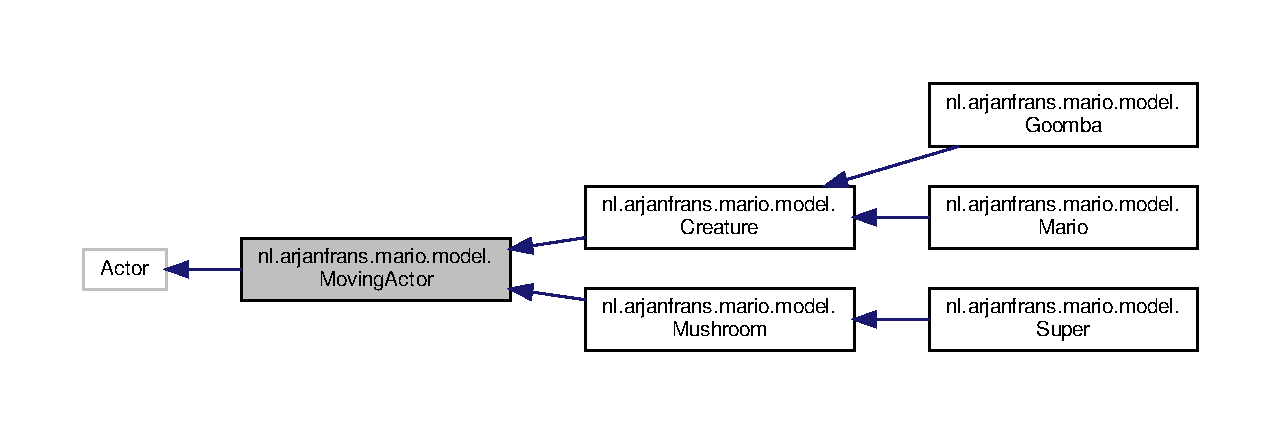
\includegraphics[width=350pt]{classnl_1_1arjanfrans_1_1mario_1_1model_1_1MovingActor__inherit__graph}
\end{center}
\end{figure}


Collaboration diagram for nl.\+arjanfrans.\+mario.\+model.\+Moving\+Actor\+:
\nopagebreak
\begin{figure}[H]
\begin{center}
\leavevmode
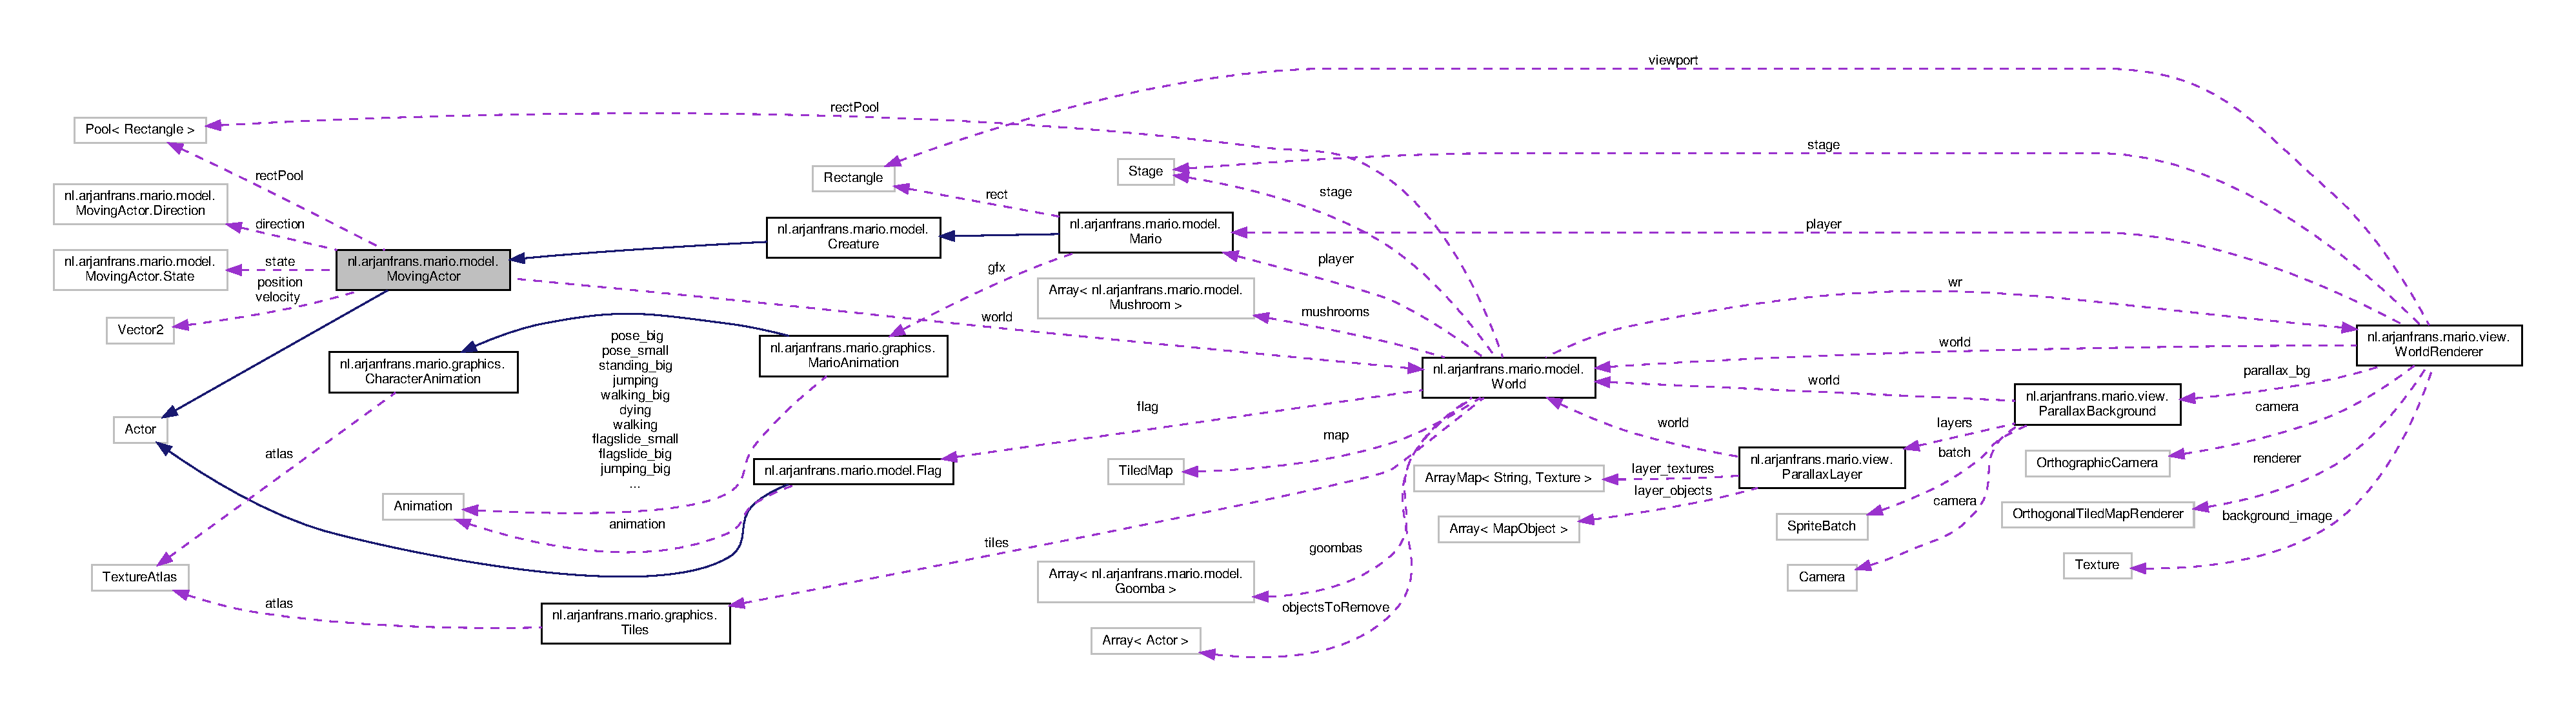
\includegraphics[width=350pt]{classnl_1_1arjanfrans_1_1mario_1_1model_1_1MovingActor__coll__graph}
\end{center}
\end{figure}
\subsection*{Classes}
\begin{DoxyCompactItemize}
\item 
enum {\bfseries Direction}
\item 
enum {\bfseries State}
\end{DoxyCompactItemize}
\subsection*{Public Member Functions}
\begin{DoxyCompactItemize}
\item 
\hyperlink{classnl_1_1arjanfrans_1_1mario_1_1model_1_1MovingActor_a56800b4b8e8457bb2e0f1a4ad38b6576}{Moving\+Actor} (\hyperlink{classnl_1_1arjanfrans_1_1mario_1_1model_1_1World}{World} world, float x, float y, float max\+\_\+velocity)
\begin{DoxyCompactList}\small\item\em Constructor method. \end{DoxyCompactList}\item 
void \hyperlink{classnl_1_1arjanfrans_1_1mario_1_1model_1_1MovingActor_a0abaf6ff6ce1a5237a268f29e433a5ed}{move} (Direction dir)
\begin{DoxyCompactList}\small\item\em This method moves the \hyperlink{classnl_1_1arjanfrans_1_1mario_1_1model_1_1MovingActor}{Moving\+Actor} in specific directions. \end{DoxyCompactList}\item 
float \hyperlink{classnl_1_1arjanfrans_1_1mario_1_1model_1_1MovingActor_a4afede59283c8dec6fcbf8ee31244320}{get\+Max\+\_\+velocity} ()
\begin{DoxyCompactList}\small\item\em This method gets the value of the max\+\_\+velocity instance variable. \end{DoxyCompactList}\item 
float \hyperlink{classnl_1_1arjanfrans_1_1mario_1_1model_1_1MovingActor_aad83e64b051035aeec7b60f32a44ea6f}{get\+Jump\+\_\+velocity} ()
\begin{DoxyCompactList}\small\item\em This method gets the value of the jump\+\_\+velocity instance variable. \end{DoxyCompactList}\item 
float \hyperlink{classnl_1_1arjanfrans_1_1mario_1_1model_1_1MovingActor_afad55ab6f56af85122985d51001e12fd}{get\+Damping} ()
\begin{DoxyCompactList}\small\item\em This method gets the daming constant in the damping instance variable. \end{DoxyCompactList}\item 
float \hyperlink{classnl_1_1arjanfrans_1_1mario_1_1model_1_1MovingActor_a2f5be4a9802efe50a98368729ab46472}{get\+State\+Time} ()
\begin{DoxyCompactList}\small\item\em This method gets the state\+Time constant in the state\+Time instance variable. \end{DoxyCompactList}\item 
boolean \hyperlink{classnl_1_1arjanfrans_1_1mario_1_1model_1_1MovingActor_a4fb6d4e3924b419bf9fb360cf2598672}{is\+Faces\+Right} ()
\begin{DoxyCompactList}\small\item\em This method gets the boolean value of the faces\+Right instance variable. \end{DoxyCompactList}\item 
Vector2 \hyperlink{classnl_1_1arjanfrans_1_1mario_1_1model_1_1MovingActor_a0ab43947ad415abb6be30ede3695b712}{get\+Velocity} ()
\begin{DoxyCompactList}\small\item\em This method gets the Vector2 object in the velocity instance variable. \end{DoxyCompactList}\item 
boolean \hyperlink{classnl_1_1arjanfrans_1_1mario_1_1model_1_1MovingActor_a43e403fe46a10dbac42c1f7800146a9c}{is\+Moving} ()
\begin{DoxyCompactList}\small\item\em This method gets the boolean value of the moving instance variable. \end{DoxyCompactList}\item 
void \hyperlink{classnl_1_1arjanfrans_1_1mario_1_1model_1_1MovingActor_af9e155f3ced19b73b253ce8f2d8f044d}{set\+Moving} (boolean moving)
\begin{DoxyCompactList}\small\item\em This method sets the boolean value of the moving instance variable. \end{DoxyCompactList}\item 
State \hyperlink{classnl_1_1arjanfrans_1_1mario_1_1model_1_1MovingActor_a40606a6b3bdc2afe43cfba764b00af4c}{get\+State} ()
\begin{DoxyCompactList}\small\item\em This method gets the state of the \hyperlink{classnl_1_1arjanfrans_1_1mario_1_1model_1_1MovingActor}{Moving\+Actor}. \end{DoxyCompactList}\item 
void \hyperlink{classnl_1_1arjanfrans_1_1mario_1_1model_1_1MovingActor_a64188e7edb074bbf9e193a8ec5fa2ec2}{set\+State} (State state)
\begin{DoxyCompactList}\small\item\em This method sets the state of the \hyperlink{classnl_1_1arjanfrans_1_1mario_1_1model_1_1MovingActor}{Moving\+Actor}. \end{DoxyCompactList}\item 
void \hyperlink{classnl_1_1arjanfrans_1_1mario_1_1model_1_1MovingActor_a331dd9271c5023d07f1840b029e703d9}{set\+Dead} (boolean dead)
\begin{DoxyCompactList}\small\item\em This method sets the boolean value of the dead instance variable. \end{DoxyCompactList}\item 
boolean \hyperlink{classnl_1_1arjanfrans_1_1mario_1_1model_1_1MovingActor_a5a5575f015d9ba97fcf344ae203f893c}{is\+Dead} ()
\begin{DoxyCompactList}\small\item\em This method gets the boolean value of the dead instance variable. \end{DoxyCompactList}\end{DoxyCompactItemize}
\subsection*{Protected Member Functions}
\begin{DoxyCompactItemize}
\item 
\mbox{\Hypertarget{classnl_1_1arjanfrans_1_1mario_1_1model_1_1MovingActor_a87133b03c2a4fd28db5d0b59f939a592}\label{classnl_1_1arjanfrans_1_1mario_1_1model_1_1MovingActor_a87133b03c2a4fd28db5d0b59f939a592}} 
Rectangle {\bfseries rectangle} ()
\item 
void \hyperlink{classnl_1_1arjanfrans_1_1mario_1_1model_1_1MovingActor_ab728cb879f42b81b171fda3ecb85260b}{apply\+Physics} (Rectangle rect)
\begin{DoxyCompactList}\small\item\em This method applies the laws of motion to a rectangle. \end{DoxyCompactList}\item 
boolean \hyperlink{classnl_1_1arjanfrans_1_1mario_1_1model_1_1MovingActor_a58d1642a39909c7f838dd84b2fb6c506}{collisionX} (Rectangle rect)
\begin{DoxyCompactList}\small\item\em This method checks if the rectangle collides with anything in the x direction. \end{DoxyCompactList}\item 
int \mbox{[}$\,$\mbox{]} \hyperlink{classnl_1_1arjanfrans_1_1mario_1_1model_1_1MovingActor_a782d932e0ff4b3b99de0542892d671c2}{check\+Tiles} (boolean checkX)
\begin{DoxyCompactList}\small\item\em This method checks for tiles in the x and y directions. \end{DoxyCompactList}\item 
void \hyperlink{classnl_1_1arjanfrans_1_1mario_1_1model_1_1MovingActor_acd9c3910d87bd94574b28599b7bc89db}{collisionY} (Rectangle rect)
\begin{DoxyCompactList}\small\item\em This method checks if the rectangle collides with anything in the y direction. \end{DoxyCompactList}\item 
Array$<$ Rectangle $>$ \hyperlink{classnl_1_1arjanfrans_1_1mario_1_1model_1_1MovingActor_a1aaf050e3c58bc9c523ccc6cefeabaf4}{get\+Tiles} (boolean isX)
\begin{DoxyCompactList}\small\item\em This method gets the tiles in the x and y directions. \end{DoxyCompactList}\item 
\mbox{\Hypertarget{classnl_1_1arjanfrans_1_1mario_1_1model_1_1MovingActor_a90b5fa37f912521b7f05f23765c5edbc}\label{classnl_1_1arjanfrans_1_1mario_1_1model_1_1MovingActor_a90b5fa37f912521b7f05f23765c5edbc}} 
void \hyperlink{classnl_1_1arjanfrans_1_1mario_1_1model_1_1MovingActor_a90b5fa37f912521b7f05f23765c5edbc}{hit\+Ground} ()
\begin{DoxyCompactList}\small\item\em This method sets the grounded boolean instance variable to true. \end{DoxyCompactList}\item 
\mbox{\Hypertarget{classnl_1_1arjanfrans_1_1mario_1_1model_1_1MovingActor_ab7c880f8d5c44d9818ee0830357a06e5}\label{classnl_1_1arjanfrans_1_1mario_1_1model_1_1MovingActor_ab7c880f8d5c44d9818ee0830357a06e5}} 
abstract void \hyperlink{classnl_1_1arjanfrans_1_1mario_1_1model_1_1MovingActor_ab7c880f8d5c44d9818ee0830357a06e5}{die\+By\+Falling} ()
\begin{DoxyCompactList}\small\item\em This method is an abstract method handled by the inherited class. \end{DoxyCompactList}\item 
\mbox{\Hypertarget{classnl_1_1arjanfrans_1_1mario_1_1model_1_1MovingActor_ac227d16626526c50745efbe666594797}\label{classnl_1_1arjanfrans_1_1mario_1_1model_1_1MovingActor_ac227d16626526c50745efbe666594797}} 
abstract void \hyperlink{classnl_1_1arjanfrans_1_1mario_1_1model_1_1MovingActor_ac227d16626526c50745efbe666594797}{collision\+X\+Action} ()
\begin{DoxyCompactList}\small\item\em This method is an abstract method handled by the inherited class. \end{DoxyCompactList}\end{DoxyCompactItemize}
\subsection*{Protected Attributes}
\begin{DoxyCompactItemize}
\item 
\mbox{\Hypertarget{classnl_1_1arjanfrans_1_1mario_1_1model_1_1MovingActor_aaecf03f3a0032c8572936fcc3da9fe70}\label{classnl_1_1arjanfrans_1_1mario_1_1model_1_1MovingActor_aaecf03f3a0032c8572936fcc3da9fe70}} 
float {\bfseries max\+\_\+velocity}
\item 
\mbox{\Hypertarget{classnl_1_1arjanfrans_1_1mario_1_1model_1_1MovingActor_a5c5b86ce3a1d5e16719c902c1dc1b1eb}\label{classnl_1_1arjanfrans_1_1mario_1_1model_1_1MovingActor_a5c5b86ce3a1d5e16719c902c1dc1b1eb}} 
float {\bfseries jump\+\_\+velocity} = 40f
\item 
\mbox{\Hypertarget{classnl_1_1arjanfrans_1_1mario_1_1model_1_1MovingActor_ae05d084bb2ae4a272bf4c6de629c606a}\label{classnl_1_1arjanfrans_1_1mario_1_1model_1_1MovingActor_ae05d084bb2ae4a272bf4c6de629c606a}} 
float {\bfseries damping} = 0.\+87f
\item 
\mbox{\Hypertarget{classnl_1_1arjanfrans_1_1mario_1_1model_1_1MovingActor_a70c7de439eef419becf4388aed28fc3b}\label{classnl_1_1arjanfrans_1_1mario_1_1model_1_1MovingActor_a70c7de439eef419becf4388aed28fc3b}} 
Vector2 {\bfseries position}
\item 
\mbox{\Hypertarget{classnl_1_1arjanfrans_1_1mario_1_1model_1_1MovingActor_a7173e8dac5804840f740fe9d357305ae}\label{classnl_1_1arjanfrans_1_1mario_1_1model_1_1MovingActor_a7173e8dac5804840f740fe9d357305ae}} 
Vector2 {\bfseries velocity}
\item 
\mbox{\Hypertarget{classnl_1_1arjanfrans_1_1mario_1_1model_1_1MovingActor_a698927fb2dd6ff4afe43561909052535}\label{classnl_1_1arjanfrans_1_1mario_1_1model_1_1MovingActor_a698927fb2dd6ff4afe43561909052535}} 
\hyperlink{classnl_1_1arjanfrans_1_1mario_1_1model_1_1World}{World} {\bfseries world}
\item 
\mbox{\Hypertarget{classnl_1_1arjanfrans_1_1mario_1_1model_1_1MovingActor_a31ad4b98d2c174817d6756e84a7fb09d}\label{classnl_1_1arjanfrans_1_1mario_1_1model_1_1MovingActor_a31ad4b98d2c174817d6756e84a7fb09d}} 
boolean {\bfseries dead}
\item 
\mbox{\Hypertarget{classnl_1_1arjanfrans_1_1mario_1_1model_1_1MovingActor_a0b6eb26ca7abec4bdc971bc842470ea0}\label{classnl_1_1arjanfrans_1_1mario_1_1model_1_1MovingActor_a0b6eb26ca7abec4bdc971bc842470ea0}} 
boolean {\bfseries moving}
\item 
\mbox{\Hypertarget{classnl_1_1arjanfrans_1_1mario_1_1model_1_1MovingActor_a21abe2ecfca8b85ae022eee104a8ab22}\label{classnl_1_1arjanfrans_1_1mario_1_1model_1_1MovingActor_a21abe2ecfca8b85ae022eee104a8ab22}} 
State {\bfseries state} = State.\+Standing
\item 
\mbox{\Hypertarget{classnl_1_1arjanfrans_1_1mario_1_1model_1_1MovingActor_a33055aba77dd7e121bcf69a2f320a531}\label{classnl_1_1arjanfrans_1_1mario_1_1model_1_1MovingActor_a33055aba77dd7e121bcf69a2f320a531}} 
float {\bfseries state\+Time} = 0
\item 
\mbox{\Hypertarget{classnl_1_1arjanfrans_1_1mario_1_1model_1_1MovingActor_afad448059900c30a0ad2ec4cfe59c097}\label{classnl_1_1arjanfrans_1_1mario_1_1model_1_1MovingActor_afad448059900c30a0ad2ec4cfe59c097}} 
int {\bfseries level}
\item 
\mbox{\Hypertarget{classnl_1_1arjanfrans_1_1mario_1_1model_1_1MovingActor_a44a86824a451864ebb36565ddde0baaa}\label{classnl_1_1arjanfrans_1_1mario_1_1model_1_1MovingActor_a44a86824a451864ebb36565ddde0baaa}} 
boolean {\bfseries faces\+Right} = true
\item 
\mbox{\Hypertarget{classnl_1_1arjanfrans_1_1mario_1_1model_1_1MovingActor_a274b212ed9a2c36f600ebb3a747582a4}\label{classnl_1_1arjanfrans_1_1mario_1_1model_1_1MovingActor_a274b212ed9a2c36f600ebb3a747582a4}} 
Direction {\bfseries direction}
\item 
\mbox{\Hypertarget{classnl_1_1arjanfrans_1_1mario_1_1model_1_1MovingActor_a152afcb89273fa62925ea2a6c1c10515}\label{classnl_1_1arjanfrans_1_1mario_1_1model_1_1MovingActor_a152afcb89273fa62925ea2a6c1c10515}} 
boolean {\bfseries grounded} = false
\item 
Pool$<$ Rectangle $>$ {\bfseries rect\+Pool}
\end{DoxyCompactItemize}


\subsection{Detailed Description}
Represents a moving actor in the game. 

\subsection{Constructor \& Destructor Documentation}
\mbox{\Hypertarget{classnl_1_1arjanfrans_1_1mario_1_1model_1_1MovingActor_a56800b4b8e8457bb2e0f1a4ad38b6576}\label{classnl_1_1arjanfrans_1_1mario_1_1model_1_1MovingActor_a56800b4b8e8457bb2e0f1a4ad38b6576}} 
\index{nl\+::arjanfrans\+::mario\+::model\+::\+Moving\+Actor@{nl\+::arjanfrans\+::mario\+::model\+::\+Moving\+Actor}!Moving\+Actor@{Moving\+Actor}}
\index{Moving\+Actor@{Moving\+Actor}!nl\+::arjanfrans\+::mario\+::model\+::\+Moving\+Actor@{nl\+::arjanfrans\+::mario\+::model\+::\+Moving\+Actor}}
\subsubsection{\texorpdfstring{Moving\+Actor()}{MovingActor()}}
{\footnotesize\ttfamily nl.\+arjanfrans.\+mario.\+model.\+Moving\+Actor.\+Moving\+Actor (\begin{DoxyParamCaption}\item[{\hyperlink{classnl_1_1arjanfrans_1_1mario_1_1model_1_1World}{World}}]{world,  }\item[{float}]{x,  }\item[{float}]{y,  }\item[{float}]{max\+\_\+velocity }\end{DoxyParamCaption})}



Constructor method. 

Method which initializes an instance of a \hyperlink{classnl_1_1arjanfrans_1_1mario_1_1model_1_1MovingActor}{Moving\+Actor} 
\begin{DoxyParams}{Parameters}
{\em world} & The world in which \hyperlink{classnl_1_1arjanfrans_1_1mario_1_1model_1_1MovingActor}{Moving\+Actor} will exist in \\
\hline
{\em x} & is the x coordinate of the position of the \hyperlink{classnl_1_1arjanfrans_1_1mario_1_1model_1_1MovingActor}{Moving\+Actor} \\
\hline
{\em y} & is the y coordinate of the position of the \hyperlink{classnl_1_1arjanfrans_1_1mario_1_1model_1_1MovingActor}{Moving\+Actor} \\
\hline
\end{DoxyParams}
\begin{DoxyReturn}{Returns}
An instance of \hyperlink{classnl_1_1arjanfrans_1_1mario_1_1model_1_1MovingActor}{Moving\+Actor} 
\end{DoxyReturn}


\subsection{Member Function Documentation}
\mbox{\Hypertarget{classnl_1_1arjanfrans_1_1mario_1_1model_1_1MovingActor_ab728cb879f42b81b171fda3ecb85260b}\label{classnl_1_1arjanfrans_1_1mario_1_1model_1_1MovingActor_ab728cb879f42b81b171fda3ecb85260b}} 
\index{nl\+::arjanfrans\+::mario\+::model\+::\+Moving\+Actor@{nl\+::arjanfrans\+::mario\+::model\+::\+Moving\+Actor}!apply\+Physics@{apply\+Physics}}
\index{apply\+Physics@{apply\+Physics}!nl\+::arjanfrans\+::mario\+::model\+::\+Moving\+Actor@{nl\+::arjanfrans\+::mario\+::model\+::\+Moving\+Actor}}
\subsubsection{\texorpdfstring{apply\+Physics()}{applyPhysics()}}
{\footnotesize\ttfamily void nl.\+arjanfrans.\+mario.\+model.\+Moving\+Actor.\+apply\+Physics (\begin{DoxyParamCaption}\item[{Rectangle}]{rect }\end{DoxyParamCaption})\hspace{0.3cm}{\ttfamily [protected]}}



This method applies the laws of motion to a rectangle. 

In the game a \hyperlink{classnl_1_1arjanfrans_1_1mario_1_1model_1_1MovingActor}{Moving\+Actor}, can be physically represented by a rectangle, so when a \hyperlink{classnl_1_1arjanfrans_1_1mario_1_1model_1_1MovingActor}{Moving\+Actor} moves the laws of physics should apply. 
\begin{DoxyParams}{Parameters}
{\em rect} & -\/ The rectangle that the \hyperlink{classnl_1_1arjanfrans_1_1mario_1_1model_1_1MovingActor}{Moving\+Actor} represents. \\
\hline
\end{DoxyParams}
\mbox{\Hypertarget{classnl_1_1arjanfrans_1_1mario_1_1model_1_1MovingActor_a782d932e0ff4b3b99de0542892d671c2}\label{classnl_1_1arjanfrans_1_1mario_1_1model_1_1MovingActor_a782d932e0ff4b3b99de0542892d671c2}} 
\index{nl\+::arjanfrans\+::mario\+::model\+::\+Moving\+Actor@{nl\+::arjanfrans\+::mario\+::model\+::\+Moving\+Actor}!check\+Tiles@{check\+Tiles}}
\index{check\+Tiles@{check\+Tiles}!nl\+::arjanfrans\+::mario\+::model\+::\+Moving\+Actor@{nl\+::arjanfrans\+::mario\+::model\+::\+Moving\+Actor}}
\subsubsection{\texorpdfstring{check\+Tiles()}{checkTiles()}}
{\footnotesize\ttfamily int \mbox{[}$\,$\mbox{]} nl.\+arjanfrans.\+mario.\+model.\+Moving\+Actor.\+check\+Tiles (\begin{DoxyParamCaption}\item[{boolean}]{checkX }\end{DoxyParamCaption})\hspace{0.3cm}{\ttfamily [protected]}}



This method checks for tiles in the x and y directions. 


\begin{DoxyParams}{Parameters}
{\em checkX} & -\/ A boolean value indicating in which direction we ar checking for tiles. \\
\hline
\end{DoxyParams}
\begin{DoxyReturn}{Returns}
an array of integers 
\end{DoxyReturn}
\mbox{\Hypertarget{classnl_1_1arjanfrans_1_1mario_1_1model_1_1MovingActor_a58d1642a39909c7f838dd84b2fb6c506}\label{classnl_1_1arjanfrans_1_1mario_1_1model_1_1MovingActor_a58d1642a39909c7f838dd84b2fb6c506}} 
\index{nl\+::arjanfrans\+::mario\+::model\+::\+Moving\+Actor@{nl\+::arjanfrans\+::mario\+::model\+::\+Moving\+Actor}!collisionX@{collisionX}}
\index{collisionX@{collisionX}!nl\+::arjanfrans\+::mario\+::model\+::\+Moving\+Actor@{nl\+::arjanfrans\+::mario\+::model\+::\+Moving\+Actor}}
\subsubsection{\texorpdfstring{collision\+X()}{collisionX()}}
{\footnotesize\ttfamily boolean nl.\+arjanfrans.\+mario.\+model.\+Moving\+Actor.\+collisionX (\begin{DoxyParamCaption}\item[{Rectangle}]{rect }\end{DoxyParamCaption})\hspace{0.3cm}{\ttfamily [protected]}}



This method checks if the rectangle collides with anything in the x direction. 

In the game a \hyperlink{classnl_1_1arjanfrans_1_1mario_1_1model_1_1MovingActor}{Moving\+Actor}, can be physically represented by a rectangle, so when a \hyperlink{classnl_1_1arjanfrans_1_1mario_1_1model_1_1MovingActor}{Moving\+Actor} meets an immovable object in x direction, the method should return true. 
\begin{DoxyParams}{Parameters}
{\em rect} & -\/ The rectangle that the \hyperlink{classnl_1_1arjanfrans_1_1mario_1_1model_1_1MovingActor}{Moving\+Actor} represents. \\
\hline
\end{DoxyParams}
\begin{DoxyReturn}{Returns}
a boolean 
\end{DoxyReturn}
\mbox{\Hypertarget{classnl_1_1arjanfrans_1_1mario_1_1model_1_1MovingActor_acd9c3910d87bd94574b28599b7bc89db}\label{classnl_1_1arjanfrans_1_1mario_1_1model_1_1MovingActor_acd9c3910d87bd94574b28599b7bc89db}} 
\index{nl\+::arjanfrans\+::mario\+::model\+::\+Moving\+Actor@{nl\+::arjanfrans\+::mario\+::model\+::\+Moving\+Actor}!collisionY@{collisionY}}
\index{collisionY@{collisionY}!nl\+::arjanfrans\+::mario\+::model\+::\+Moving\+Actor@{nl\+::arjanfrans\+::mario\+::model\+::\+Moving\+Actor}}
\subsubsection{\texorpdfstring{collision\+Y()}{collisionY()}}
{\footnotesize\ttfamily void nl.\+arjanfrans.\+mario.\+model.\+Moving\+Actor.\+collisionY (\begin{DoxyParamCaption}\item[{Rectangle}]{rect }\end{DoxyParamCaption})\hspace{0.3cm}{\ttfamily [protected]}}



This method checks if the rectangle collides with anything in the y direction. 

In the game a \hyperlink{classnl_1_1arjanfrans_1_1mario_1_1model_1_1MovingActor}{Moving\+Actor}, can be physically represented by a rectangle, so when a \hyperlink{classnl_1_1arjanfrans_1_1mario_1_1model_1_1MovingActor}{Moving\+Actor} meets an immovable object in y direction, the method should return true. 
\begin{DoxyParams}{Parameters}
{\em rect} & -\/ The rectangle that the \hyperlink{classnl_1_1arjanfrans_1_1mario_1_1model_1_1MovingActor}{Moving\+Actor} represents. \\
\hline
\end{DoxyParams}
\begin{DoxyReturn}{Returns}
a boolean 
\end{DoxyReturn}
\mbox{\Hypertarget{classnl_1_1arjanfrans_1_1mario_1_1model_1_1MovingActor_afad55ab6f56af85122985d51001e12fd}\label{classnl_1_1arjanfrans_1_1mario_1_1model_1_1MovingActor_afad55ab6f56af85122985d51001e12fd}} 
\index{nl\+::arjanfrans\+::mario\+::model\+::\+Moving\+Actor@{nl\+::arjanfrans\+::mario\+::model\+::\+Moving\+Actor}!get\+Damping@{get\+Damping}}
\index{get\+Damping@{get\+Damping}!nl\+::arjanfrans\+::mario\+::model\+::\+Moving\+Actor@{nl\+::arjanfrans\+::mario\+::model\+::\+Moving\+Actor}}
\subsubsection{\texorpdfstring{get\+Damping()}{getDamping()}}
{\footnotesize\ttfamily float nl.\+arjanfrans.\+mario.\+model.\+Moving\+Actor.\+get\+Damping (\begin{DoxyParamCaption}{ }\end{DoxyParamCaption})}



This method gets the daming constant in the damping instance variable. 

\begin{DoxyReturn}{Returns}
a float representing the damping constant. 
\end{DoxyReturn}
\mbox{\Hypertarget{classnl_1_1arjanfrans_1_1mario_1_1model_1_1MovingActor_aad83e64b051035aeec7b60f32a44ea6f}\label{classnl_1_1arjanfrans_1_1mario_1_1model_1_1MovingActor_aad83e64b051035aeec7b60f32a44ea6f}} 
\index{nl\+::arjanfrans\+::mario\+::model\+::\+Moving\+Actor@{nl\+::arjanfrans\+::mario\+::model\+::\+Moving\+Actor}!get\+Jump\+\_\+velocity@{get\+Jump\+\_\+velocity}}
\index{get\+Jump\+\_\+velocity@{get\+Jump\+\_\+velocity}!nl\+::arjanfrans\+::mario\+::model\+::\+Moving\+Actor@{nl\+::arjanfrans\+::mario\+::model\+::\+Moving\+Actor}}
\subsubsection{\texorpdfstring{get\+Jump\+\_\+velocity()}{getJump\_velocity()}}
{\footnotesize\ttfamily float nl.\+arjanfrans.\+mario.\+model.\+Moving\+Actor.\+get\+Jump\+\_\+velocity (\begin{DoxyParamCaption}{ }\end{DoxyParamCaption})}



This method gets the value of the jump\+\_\+velocity instance variable. 

\begin{DoxyReturn}{Returns}
a float representing the jump velocity. 
\end{DoxyReturn}
\mbox{\Hypertarget{classnl_1_1arjanfrans_1_1mario_1_1model_1_1MovingActor_a4afede59283c8dec6fcbf8ee31244320}\label{classnl_1_1arjanfrans_1_1mario_1_1model_1_1MovingActor_a4afede59283c8dec6fcbf8ee31244320}} 
\index{nl\+::arjanfrans\+::mario\+::model\+::\+Moving\+Actor@{nl\+::arjanfrans\+::mario\+::model\+::\+Moving\+Actor}!get\+Max\+\_\+velocity@{get\+Max\+\_\+velocity}}
\index{get\+Max\+\_\+velocity@{get\+Max\+\_\+velocity}!nl\+::arjanfrans\+::mario\+::model\+::\+Moving\+Actor@{nl\+::arjanfrans\+::mario\+::model\+::\+Moving\+Actor}}
\subsubsection{\texorpdfstring{get\+Max\+\_\+velocity()}{getMax\_velocity()}}
{\footnotesize\ttfamily float nl.\+arjanfrans.\+mario.\+model.\+Moving\+Actor.\+get\+Max\+\_\+velocity (\begin{DoxyParamCaption}{ }\end{DoxyParamCaption})}



This method gets the value of the max\+\_\+velocity instance variable. 

\begin{DoxyReturn}{Returns}
a float representing the max velocity. 
\end{DoxyReturn}
\mbox{\Hypertarget{classnl_1_1arjanfrans_1_1mario_1_1model_1_1MovingActor_a40606a6b3bdc2afe43cfba764b00af4c}\label{classnl_1_1arjanfrans_1_1mario_1_1model_1_1MovingActor_a40606a6b3bdc2afe43cfba764b00af4c}} 
\index{nl\+::arjanfrans\+::mario\+::model\+::\+Moving\+Actor@{nl\+::arjanfrans\+::mario\+::model\+::\+Moving\+Actor}!get\+State@{get\+State}}
\index{get\+State@{get\+State}!nl\+::arjanfrans\+::mario\+::model\+::\+Moving\+Actor@{nl\+::arjanfrans\+::mario\+::model\+::\+Moving\+Actor}}
\subsubsection{\texorpdfstring{get\+State()}{getState()}}
{\footnotesize\ttfamily State nl.\+arjanfrans.\+mario.\+model.\+Moving\+Actor.\+get\+State (\begin{DoxyParamCaption}{ }\end{DoxyParamCaption})}



This method gets the state of the \hyperlink{classnl_1_1arjanfrans_1_1mario_1_1model_1_1MovingActor}{Moving\+Actor}. 

\begin{DoxyReturn}{Returns}
a member of the State enumernation class representing what the \hyperlink{classnl_1_1arjanfrans_1_1mario_1_1model_1_1MovingActor}{Moving\+Actor} is doing. 
\end{DoxyReturn}
\mbox{\Hypertarget{classnl_1_1arjanfrans_1_1mario_1_1model_1_1MovingActor_a2f5be4a9802efe50a98368729ab46472}\label{classnl_1_1arjanfrans_1_1mario_1_1model_1_1MovingActor_a2f5be4a9802efe50a98368729ab46472}} 
\index{nl\+::arjanfrans\+::mario\+::model\+::\+Moving\+Actor@{nl\+::arjanfrans\+::mario\+::model\+::\+Moving\+Actor}!get\+State\+Time@{get\+State\+Time}}
\index{get\+State\+Time@{get\+State\+Time}!nl\+::arjanfrans\+::mario\+::model\+::\+Moving\+Actor@{nl\+::arjanfrans\+::mario\+::model\+::\+Moving\+Actor}}
\subsubsection{\texorpdfstring{get\+State\+Time()}{getStateTime()}}
{\footnotesize\ttfamily float nl.\+arjanfrans.\+mario.\+model.\+Moving\+Actor.\+get\+State\+Time (\begin{DoxyParamCaption}{ }\end{DoxyParamCaption})}



This method gets the state\+Time constant in the state\+Time instance variable. 

\begin{DoxyReturn}{Returns}
a float representing the state time. 
\end{DoxyReturn}
\mbox{\Hypertarget{classnl_1_1arjanfrans_1_1mario_1_1model_1_1MovingActor_a1aaf050e3c58bc9c523ccc6cefeabaf4}\label{classnl_1_1arjanfrans_1_1mario_1_1model_1_1MovingActor_a1aaf050e3c58bc9c523ccc6cefeabaf4}} 
\index{nl\+::arjanfrans\+::mario\+::model\+::\+Moving\+Actor@{nl\+::arjanfrans\+::mario\+::model\+::\+Moving\+Actor}!get\+Tiles@{get\+Tiles}}
\index{get\+Tiles@{get\+Tiles}!nl\+::arjanfrans\+::mario\+::model\+::\+Moving\+Actor@{nl\+::arjanfrans\+::mario\+::model\+::\+Moving\+Actor}}
\subsubsection{\texorpdfstring{get\+Tiles()}{getTiles()}}
{\footnotesize\ttfamily Array$<$Rectangle$>$ nl.\+arjanfrans.\+mario.\+model.\+Moving\+Actor.\+get\+Tiles (\begin{DoxyParamCaption}\item[{boolean}]{isX }\end{DoxyParamCaption})\hspace{0.3cm}{\ttfamily [protected]}}



This method gets the tiles in the x and y directions. 


\begin{DoxyParams}{Parameters}
{\em isX} & -\/ A boolean value indicating the direction in which the tile are being retrieved. \\
\hline
\end{DoxyParams}
\begin{DoxyReturn}{Returns}
an array of Rectangle objects 
\end{DoxyReturn}
\mbox{\Hypertarget{classnl_1_1arjanfrans_1_1mario_1_1model_1_1MovingActor_a0ab43947ad415abb6be30ede3695b712}\label{classnl_1_1arjanfrans_1_1mario_1_1model_1_1MovingActor_a0ab43947ad415abb6be30ede3695b712}} 
\index{nl\+::arjanfrans\+::mario\+::model\+::\+Moving\+Actor@{nl\+::arjanfrans\+::mario\+::model\+::\+Moving\+Actor}!get\+Velocity@{get\+Velocity}}
\index{get\+Velocity@{get\+Velocity}!nl\+::arjanfrans\+::mario\+::model\+::\+Moving\+Actor@{nl\+::arjanfrans\+::mario\+::model\+::\+Moving\+Actor}}
\subsubsection{\texorpdfstring{get\+Velocity()}{getVelocity()}}
{\footnotesize\ttfamily Vector2 nl.\+arjanfrans.\+mario.\+model.\+Moving\+Actor.\+get\+Velocity (\begin{DoxyParamCaption}{ }\end{DoxyParamCaption})}



This method gets the Vector2 object in the velocity instance variable. 

\begin{DoxyReturn}{Returns}
a Vector2 object representing the velocity of a \hyperlink{classnl_1_1arjanfrans_1_1mario_1_1model_1_1MovingActor}{Moving\+Actor}. 
\end{DoxyReturn}
\mbox{\Hypertarget{classnl_1_1arjanfrans_1_1mario_1_1model_1_1MovingActor_a5a5575f015d9ba97fcf344ae203f893c}\label{classnl_1_1arjanfrans_1_1mario_1_1model_1_1MovingActor_a5a5575f015d9ba97fcf344ae203f893c}} 
\index{nl\+::arjanfrans\+::mario\+::model\+::\+Moving\+Actor@{nl\+::arjanfrans\+::mario\+::model\+::\+Moving\+Actor}!is\+Dead@{is\+Dead}}
\index{is\+Dead@{is\+Dead}!nl\+::arjanfrans\+::mario\+::model\+::\+Moving\+Actor@{nl\+::arjanfrans\+::mario\+::model\+::\+Moving\+Actor}}
\subsubsection{\texorpdfstring{is\+Dead()}{isDead()}}
{\footnotesize\ttfamily boolean nl.\+arjanfrans.\+mario.\+model.\+Moving\+Actor.\+is\+Dead (\begin{DoxyParamCaption}{ }\end{DoxyParamCaption})}



This method gets the boolean value of the dead instance variable. 

\begin{DoxyReturn}{Returns}
a boolean representing whether the \hyperlink{classnl_1_1arjanfrans_1_1mario_1_1model_1_1MovingActor}{Moving\+Actor} is dead or not. 
\end{DoxyReturn}
\mbox{\Hypertarget{classnl_1_1arjanfrans_1_1mario_1_1model_1_1MovingActor_a4fb6d4e3924b419bf9fb360cf2598672}\label{classnl_1_1arjanfrans_1_1mario_1_1model_1_1MovingActor_a4fb6d4e3924b419bf9fb360cf2598672}} 
\index{nl\+::arjanfrans\+::mario\+::model\+::\+Moving\+Actor@{nl\+::arjanfrans\+::mario\+::model\+::\+Moving\+Actor}!is\+Faces\+Right@{is\+Faces\+Right}}
\index{is\+Faces\+Right@{is\+Faces\+Right}!nl\+::arjanfrans\+::mario\+::model\+::\+Moving\+Actor@{nl\+::arjanfrans\+::mario\+::model\+::\+Moving\+Actor}}
\subsubsection{\texorpdfstring{is\+Faces\+Right()}{isFacesRight()}}
{\footnotesize\ttfamily boolean nl.\+arjanfrans.\+mario.\+model.\+Moving\+Actor.\+is\+Faces\+Right (\begin{DoxyParamCaption}{ }\end{DoxyParamCaption})}



This method gets the boolean value of the faces\+Right instance variable. 

\begin{DoxyReturn}{Returns}
a boolean representing which way the \hyperlink{classnl_1_1arjanfrans_1_1mario_1_1model_1_1MovingActor}{Moving\+Actor} faces. 
\end{DoxyReturn}
\mbox{\Hypertarget{classnl_1_1arjanfrans_1_1mario_1_1model_1_1MovingActor_a43e403fe46a10dbac42c1f7800146a9c}\label{classnl_1_1arjanfrans_1_1mario_1_1model_1_1MovingActor_a43e403fe46a10dbac42c1f7800146a9c}} 
\index{nl\+::arjanfrans\+::mario\+::model\+::\+Moving\+Actor@{nl\+::arjanfrans\+::mario\+::model\+::\+Moving\+Actor}!is\+Moving@{is\+Moving}}
\index{is\+Moving@{is\+Moving}!nl\+::arjanfrans\+::mario\+::model\+::\+Moving\+Actor@{nl\+::arjanfrans\+::mario\+::model\+::\+Moving\+Actor}}
\subsubsection{\texorpdfstring{is\+Moving()}{isMoving()}}
{\footnotesize\ttfamily boolean nl.\+arjanfrans.\+mario.\+model.\+Moving\+Actor.\+is\+Moving (\begin{DoxyParamCaption}{ }\end{DoxyParamCaption})}



This method gets the boolean value of the moving instance variable. 

\begin{DoxyReturn}{Returns}
a boolean representing whether the \hyperlink{classnl_1_1arjanfrans_1_1mario_1_1model_1_1MovingActor}{Moving\+Actor} is in motion. 
\end{DoxyReturn}
\mbox{\Hypertarget{classnl_1_1arjanfrans_1_1mario_1_1model_1_1MovingActor_a0abaf6ff6ce1a5237a268f29e433a5ed}\label{classnl_1_1arjanfrans_1_1mario_1_1model_1_1MovingActor_a0abaf6ff6ce1a5237a268f29e433a5ed}} 
\index{nl\+::arjanfrans\+::mario\+::model\+::\+Moving\+Actor@{nl\+::arjanfrans\+::mario\+::model\+::\+Moving\+Actor}!move@{move}}
\index{move@{move}!nl\+::arjanfrans\+::mario\+::model\+::\+Moving\+Actor@{nl\+::arjanfrans\+::mario\+::model\+::\+Moving\+Actor}}
\subsubsection{\texorpdfstring{move()}{move()}}
{\footnotesize\ttfamily void nl.\+arjanfrans.\+mario.\+model.\+Moving\+Actor.\+move (\begin{DoxyParamCaption}\item[{Direction}]{dir }\end{DoxyParamCaption})}



This method moves the \hyperlink{classnl_1_1arjanfrans_1_1mario_1_1model_1_1MovingActor}{Moving\+Actor} in specific directions. 

When on the ground a \hyperlink{classnl_1_1arjanfrans_1_1mario_1_1model_1_1MovingActor}{Moving\+Actor} can be move in two directions, either left or right 
\begin{DoxyParams}{Parameters}
{\em dir} & -\/ A direction listed in the enumeration class called Direction. \\
\hline
\end{DoxyParams}
\mbox{\Hypertarget{classnl_1_1arjanfrans_1_1mario_1_1model_1_1MovingActor_a331dd9271c5023d07f1840b029e703d9}\label{classnl_1_1arjanfrans_1_1mario_1_1model_1_1MovingActor_a331dd9271c5023d07f1840b029e703d9}} 
\index{nl\+::arjanfrans\+::mario\+::model\+::\+Moving\+Actor@{nl\+::arjanfrans\+::mario\+::model\+::\+Moving\+Actor}!set\+Dead@{set\+Dead}}
\index{set\+Dead@{set\+Dead}!nl\+::arjanfrans\+::mario\+::model\+::\+Moving\+Actor@{nl\+::arjanfrans\+::mario\+::model\+::\+Moving\+Actor}}
\subsubsection{\texorpdfstring{set\+Dead()}{setDead()}}
{\footnotesize\ttfamily void nl.\+arjanfrans.\+mario.\+model.\+Moving\+Actor.\+set\+Dead (\begin{DoxyParamCaption}\item[{boolean}]{dead }\end{DoxyParamCaption})}



This method sets the boolean value of the dead instance variable. 


\begin{DoxyParams}{Parameters}
{\em a} & boolean representing whether the \hyperlink{classnl_1_1arjanfrans_1_1mario_1_1model_1_1MovingActor}{Moving\+Actor} is dead or not. \\
\hline
\end{DoxyParams}
\mbox{\Hypertarget{classnl_1_1arjanfrans_1_1mario_1_1model_1_1MovingActor_af9e155f3ced19b73b253ce8f2d8f044d}\label{classnl_1_1arjanfrans_1_1mario_1_1model_1_1MovingActor_af9e155f3ced19b73b253ce8f2d8f044d}} 
\index{nl\+::arjanfrans\+::mario\+::model\+::\+Moving\+Actor@{nl\+::arjanfrans\+::mario\+::model\+::\+Moving\+Actor}!set\+Moving@{set\+Moving}}
\index{set\+Moving@{set\+Moving}!nl\+::arjanfrans\+::mario\+::model\+::\+Moving\+Actor@{nl\+::arjanfrans\+::mario\+::model\+::\+Moving\+Actor}}
\subsubsection{\texorpdfstring{set\+Moving()}{setMoving()}}
{\footnotesize\ttfamily void nl.\+arjanfrans.\+mario.\+model.\+Moving\+Actor.\+set\+Moving (\begin{DoxyParamCaption}\item[{boolean}]{moving }\end{DoxyParamCaption})}



This method sets the boolean value of the moving instance variable. 


\begin{DoxyParams}{Parameters}
{\em moving} & -\/ a boolean indicating whether the Movign\+Actor is in motion. \\
\hline
\end{DoxyParams}
\mbox{\Hypertarget{classnl_1_1arjanfrans_1_1mario_1_1model_1_1MovingActor_a64188e7edb074bbf9e193a8ec5fa2ec2}\label{classnl_1_1arjanfrans_1_1mario_1_1model_1_1MovingActor_a64188e7edb074bbf9e193a8ec5fa2ec2}} 
\index{nl\+::arjanfrans\+::mario\+::model\+::\+Moving\+Actor@{nl\+::arjanfrans\+::mario\+::model\+::\+Moving\+Actor}!set\+State@{set\+State}}
\index{set\+State@{set\+State}!nl\+::arjanfrans\+::mario\+::model\+::\+Moving\+Actor@{nl\+::arjanfrans\+::mario\+::model\+::\+Moving\+Actor}}
\subsubsection{\texorpdfstring{set\+State()}{setState()}}
{\footnotesize\ttfamily void nl.\+arjanfrans.\+mario.\+model.\+Moving\+Actor.\+set\+State (\begin{DoxyParamCaption}\item[{State}]{state }\end{DoxyParamCaption})}



This method sets the state of the \hyperlink{classnl_1_1arjanfrans_1_1mario_1_1model_1_1MovingActor}{Moving\+Actor}. 


\begin{DoxyParams}{Parameters}
{\em a} & member of the State enumernation class representing what the \hyperlink{classnl_1_1arjanfrans_1_1mario_1_1model_1_1MovingActor}{Moving\+Actor} is doing. \\
\hline
\end{DoxyParams}


\subsection{Member Data Documentation}
\mbox{\Hypertarget{classnl_1_1arjanfrans_1_1mario_1_1model_1_1MovingActor_a4c472abc5e7932e72845bcc0d94a3e45}\label{classnl_1_1arjanfrans_1_1mario_1_1model_1_1MovingActor_a4c472abc5e7932e72845bcc0d94a3e45}} 
\index{nl\+::arjanfrans\+::mario\+::model\+::\+Moving\+Actor@{nl\+::arjanfrans\+::mario\+::model\+::\+Moving\+Actor}!rect\+Pool@{rect\+Pool}}
\index{rect\+Pool@{rect\+Pool}!nl\+::arjanfrans\+::mario\+::model\+::\+Moving\+Actor@{nl\+::arjanfrans\+::mario\+::model\+::\+Moving\+Actor}}
\subsubsection{\texorpdfstring{rect\+Pool}{rectPool}}
{\footnotesize\ttfamily Pool$<$Rectangle$>$ nl.\+arjanfrans.\+mario.\+model.\+Moving\+Actor.\+rect\+Pool\hspace{0.3cm}{\ttfamily [protected]}}

{\bfseries Initial value\+:}
\begin{DoxyCode}
= \textcolor{keyword}{new} Pool<Rectangle>() \{
        @Override
        \textcolor{keyword}{protected} Rectangle newObject() \{
            \textcolor{keywordflow}{return} \textcolor{keyword}{new} Rectangle();
        \}
    \}
\end{DoxyCode}


The documentation for this class was generated from the following file\+:\begin{DoxyCompactItemize}
\item 
core/src/nl/arjanfrans/mario/model/Moving\+Actor.\+java\end{DoxyCompactItemize}

\hypertarget{classnl_1_1arjanfrans_1_1mario_1_1model_1_1Mushroom}{}\section{nl.\+arjanfrans.\+mario.\+model.\+Mushroom Class Reference}
\label{classnl_1_1arjanfrans_1_1mario_1_1model_1_1Mushroom}\index{nl.\+arjanfrans.\+mario.\+model.\+Mushroom@{nl.\+arjanfrans.\+mario.\+model.\+Mushroom}}


Inherited class \hyperlink{classnl_1_1arjanfrans_1_1mario_1_1model_1_1MovingActor}{Moving\+Actor}.  




Inheritance diagram for nl.\+arjanfrans.\+mario.\+model.\+Mushroom\+:
\nopagebreak
\begin{figure}[H]
\begin{center}
\leavevmode
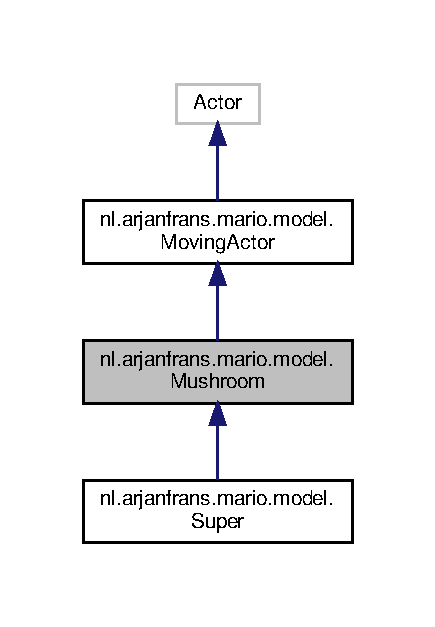
\includegraphics[width=209pt]{classnl_1_1arjanfrans_1_1mario_1_1model_1_1Mushroom__inherit__graph}
\end{center}
\end{figure}


Collaboration diagram for nl.\+arjanfrans.\+mario.\+model.\+Mushroom\+:
\nopagebreak
\begin{figure}[H]
\begin{center}
\leavevmode
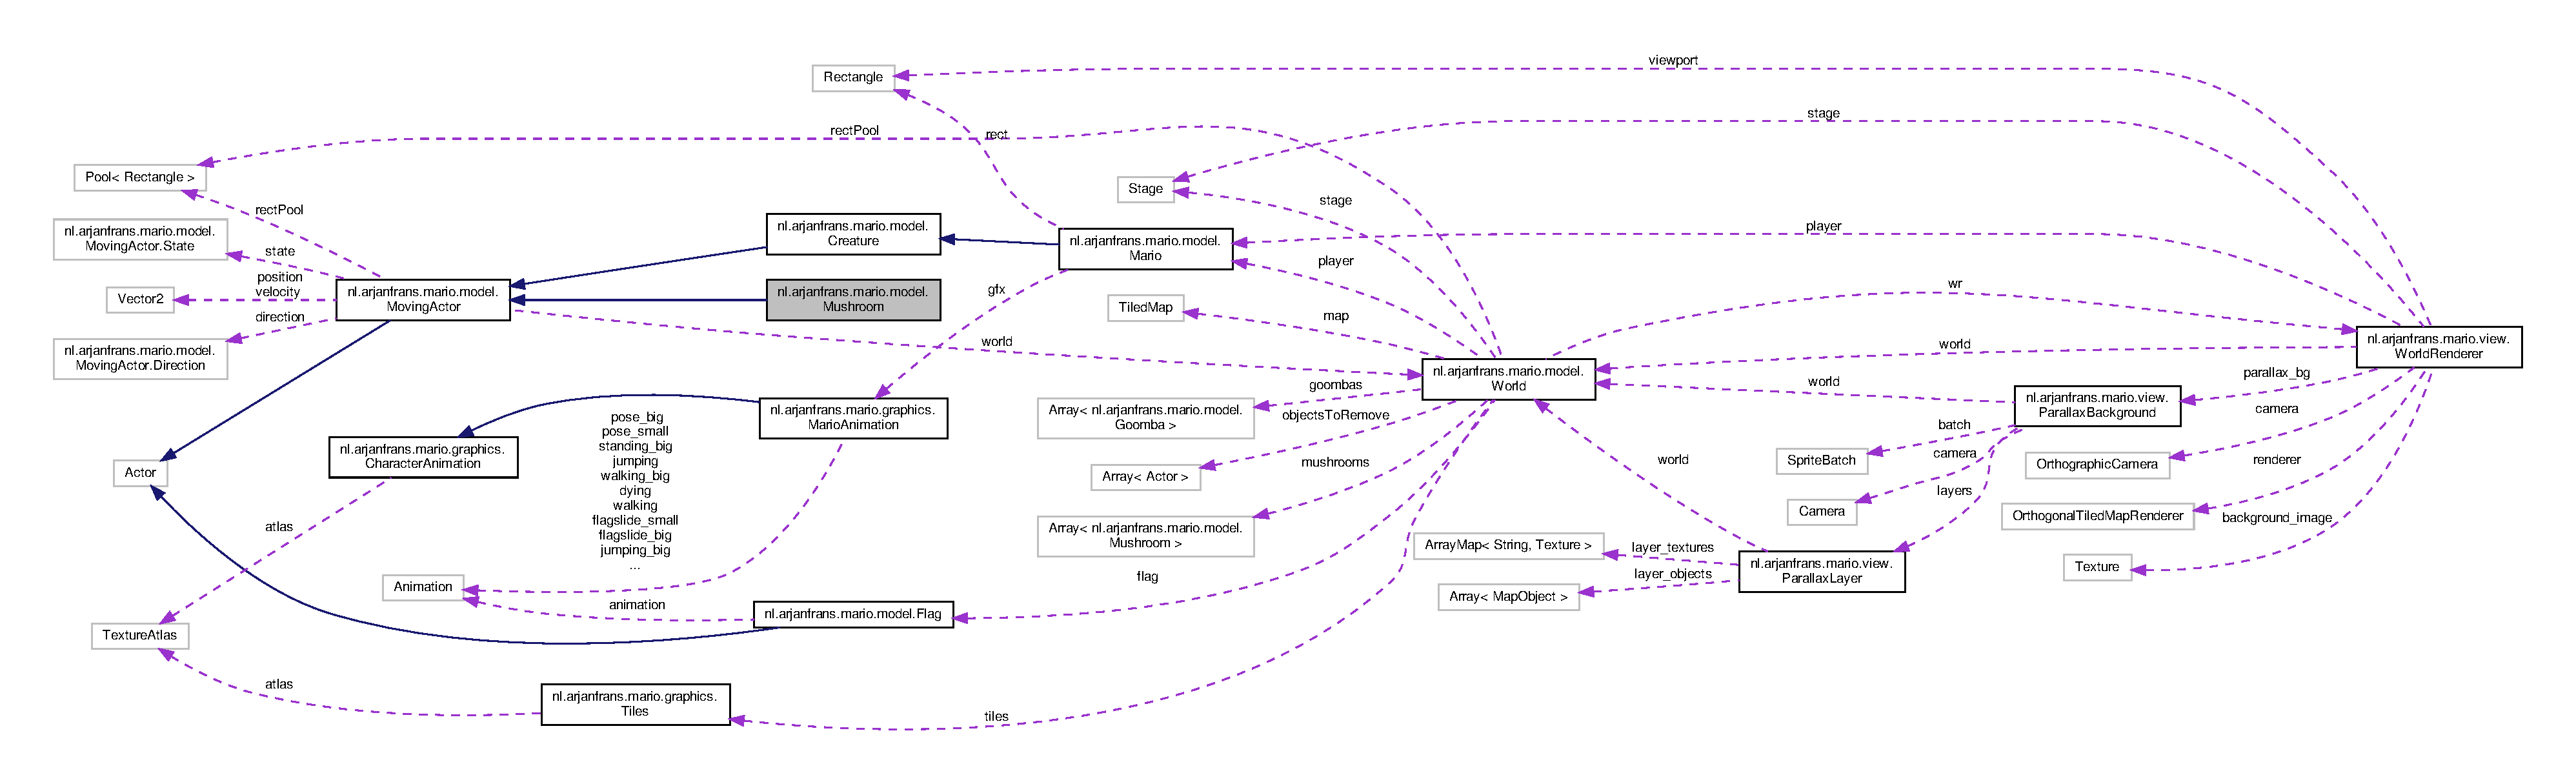
\includegraphics[width=350pt]{classnl_1_1arjanfrans_1_1mario_1_1model_1_1Mushroom__coll__graph}
\end{center}
\end{figure}
\subsection*{Public Member Functions}
\begin{DoxyCompactItemize}
\item 
\hyperlink{classnl_1_1arjanfrans_1_1mario_1_1model_1_1Mushroom_a0989b16e9c3061a514c25d1193c628e5}{Mushroom} (\hyperlink{classnl_1_1arjanfrans_1_1mario_1_1model_1_1World}{World} world, float x, float y, float max\+\_\+velocity)
\begin{DoxyCompactList}\small\item\em Constructor method. \end{DoxyCompactList}\item 
\mbox{\Hypertarget{classnl_1_1arjanfrans_1_1mario_1_1model_1_1Mushroom_a79a92038e1a869bbfd696839442dbae5}\label{classnl_1_1arjanfrans_1_1mario_1_1model_1_1Mushroom_a79a92038e1a869bbfd696839442dbae5}} 
void \hyperlink{classnl_1_1arjanfrans_1_1mario_1_1model_1_1Mushroom_a79a92038e1a869bbfd696839442dbae5}{appear} ()
\begin{DoxyCompactList}\small\item\em Make mushroom appear. \end{DoxyCompactList}\item 
\mbox{\Hypertarget{classnl_1_1arjanfrans_1_1mario_1_1model_1_1Mushroom_a145a3bd421ab31131a842ac9bab03021}\label{classnl_1_1arjanfrans_1_1mario_1_1model_1_1Mushroom_a145a3bd421ab31131a842ac9bab03021}} 
abstract void \hyperlink{classnl_1_1arjanfrans_1_1mario_1_1model_1_1Mushroom_a145a3bd421ab31131a842ac9bab03021}{dispose} ()
\begin{DoxyCompactList}\small\item\em Dispose mushroom. \end{DoxyCompactList}\end{DoxyCompactItemize}
\subsection*{Additional Inherited Members}


\subsection{Detailed Description}
Inherited class \hyperlink{classnl_1_1arjanfrans_1_1mario_1_1model_1_1MovingActor}{Moving\+Actor}. 

\subsection{Constructor \& Destructor Documentation}
\mbox{\Hypertarget{classnl_1_1arjanfrans_1_1mario_1_1model_1_1Mushroom_a0989b16e9c3061a514c25d1193c628e5}\label{classnl_1_1arjanfrans_1_1mario_1_1model_1_1Mushroom_a0989b16e9c3061a514c25d1193c628e5}} 
\index{nl\+::arjanfrans\+::mario\+::model\+::\+Mushroom@{nl\+::arjanfrans\+::mario\+::model\+::\+Mushroom}!Mushroom@{Mushroom}}
\index{Mushroom@{Mushroom}!nl\+::arjanfrans\+::mario\+::model\+::\+Mushroom@{nl\+::arjanfrans\+::mario\+::model\+::\+Mushroom}}
\subsubsection{\texorpdfstring{Mushroom()}{Mushroom()}}
{\footnotesize\ttfamily nl.\+arjanfrans.\+mario.\+model.\+Mushroom.\+Mushroom (\begin{DoxyParamCaption}\item[{\hyperlink{classnl_1_1arjanfrans_1_1mario_1_1model_1_1World}{World}}]{world,  }\item[{float}]{x,  }\item[{float}]{y,  }\item[{float}]{max\+\_\+velocity }\end{DoxyParamCaption})}



Constructor method. 

Method which initializes an instance of \hyperlink{classnl_1_1arjanfrans_1_1mario_1_1model_1_1StaticActor}{Static\+Actor} 
\begin{DoxyParams}{Parameters}
{\em world} & The world object in which \hyperlink{classnl_1_1arjanfrans_1_1mario_1_1model_1_1Mario}{Mario} will exist in \\
\hline
{\em x} & coordinate \\
\hline
{\em y} & coordinate \\
\hline
{\em max\+\_\+velocity} & \\
\hline
\end{DoxyParams}


The documentation for this class was generated from the following file\+:\begin{DoxyCompactItemize}
\item 
core/src/nl/arjanfrans/mario/model/\hyperlink{Mushroom_8java}{Mushroom.\+java}\end{DoxyCompactItemize}

\hypertarget{classnl_1_1arjanfrans_1_1mario_1_1view_1_1ParallaxBackground}{}\section{nl.\+arjanfrans.\+mario.\+view.\+Parallax\+Background Class Reference}
\label{classnl_1_1arjanfrans_1_1mario_1_1view_1_1ParallaxBackground}\index{nl.\+arjanfrans.\+mario.\+view.\+Parallax\+Background@{nl.\+arjanfrans.\+mario.\+view.\+Parallax\+Background}}


The class meant to create a parallax background.  




Collaboration diagram for nl.\+arjanfrans.\+mario.\+view.\+Parallax\+Background\+:
\nopagebreak
\begin{figure}[H]
\begin{center}
\leavevmode
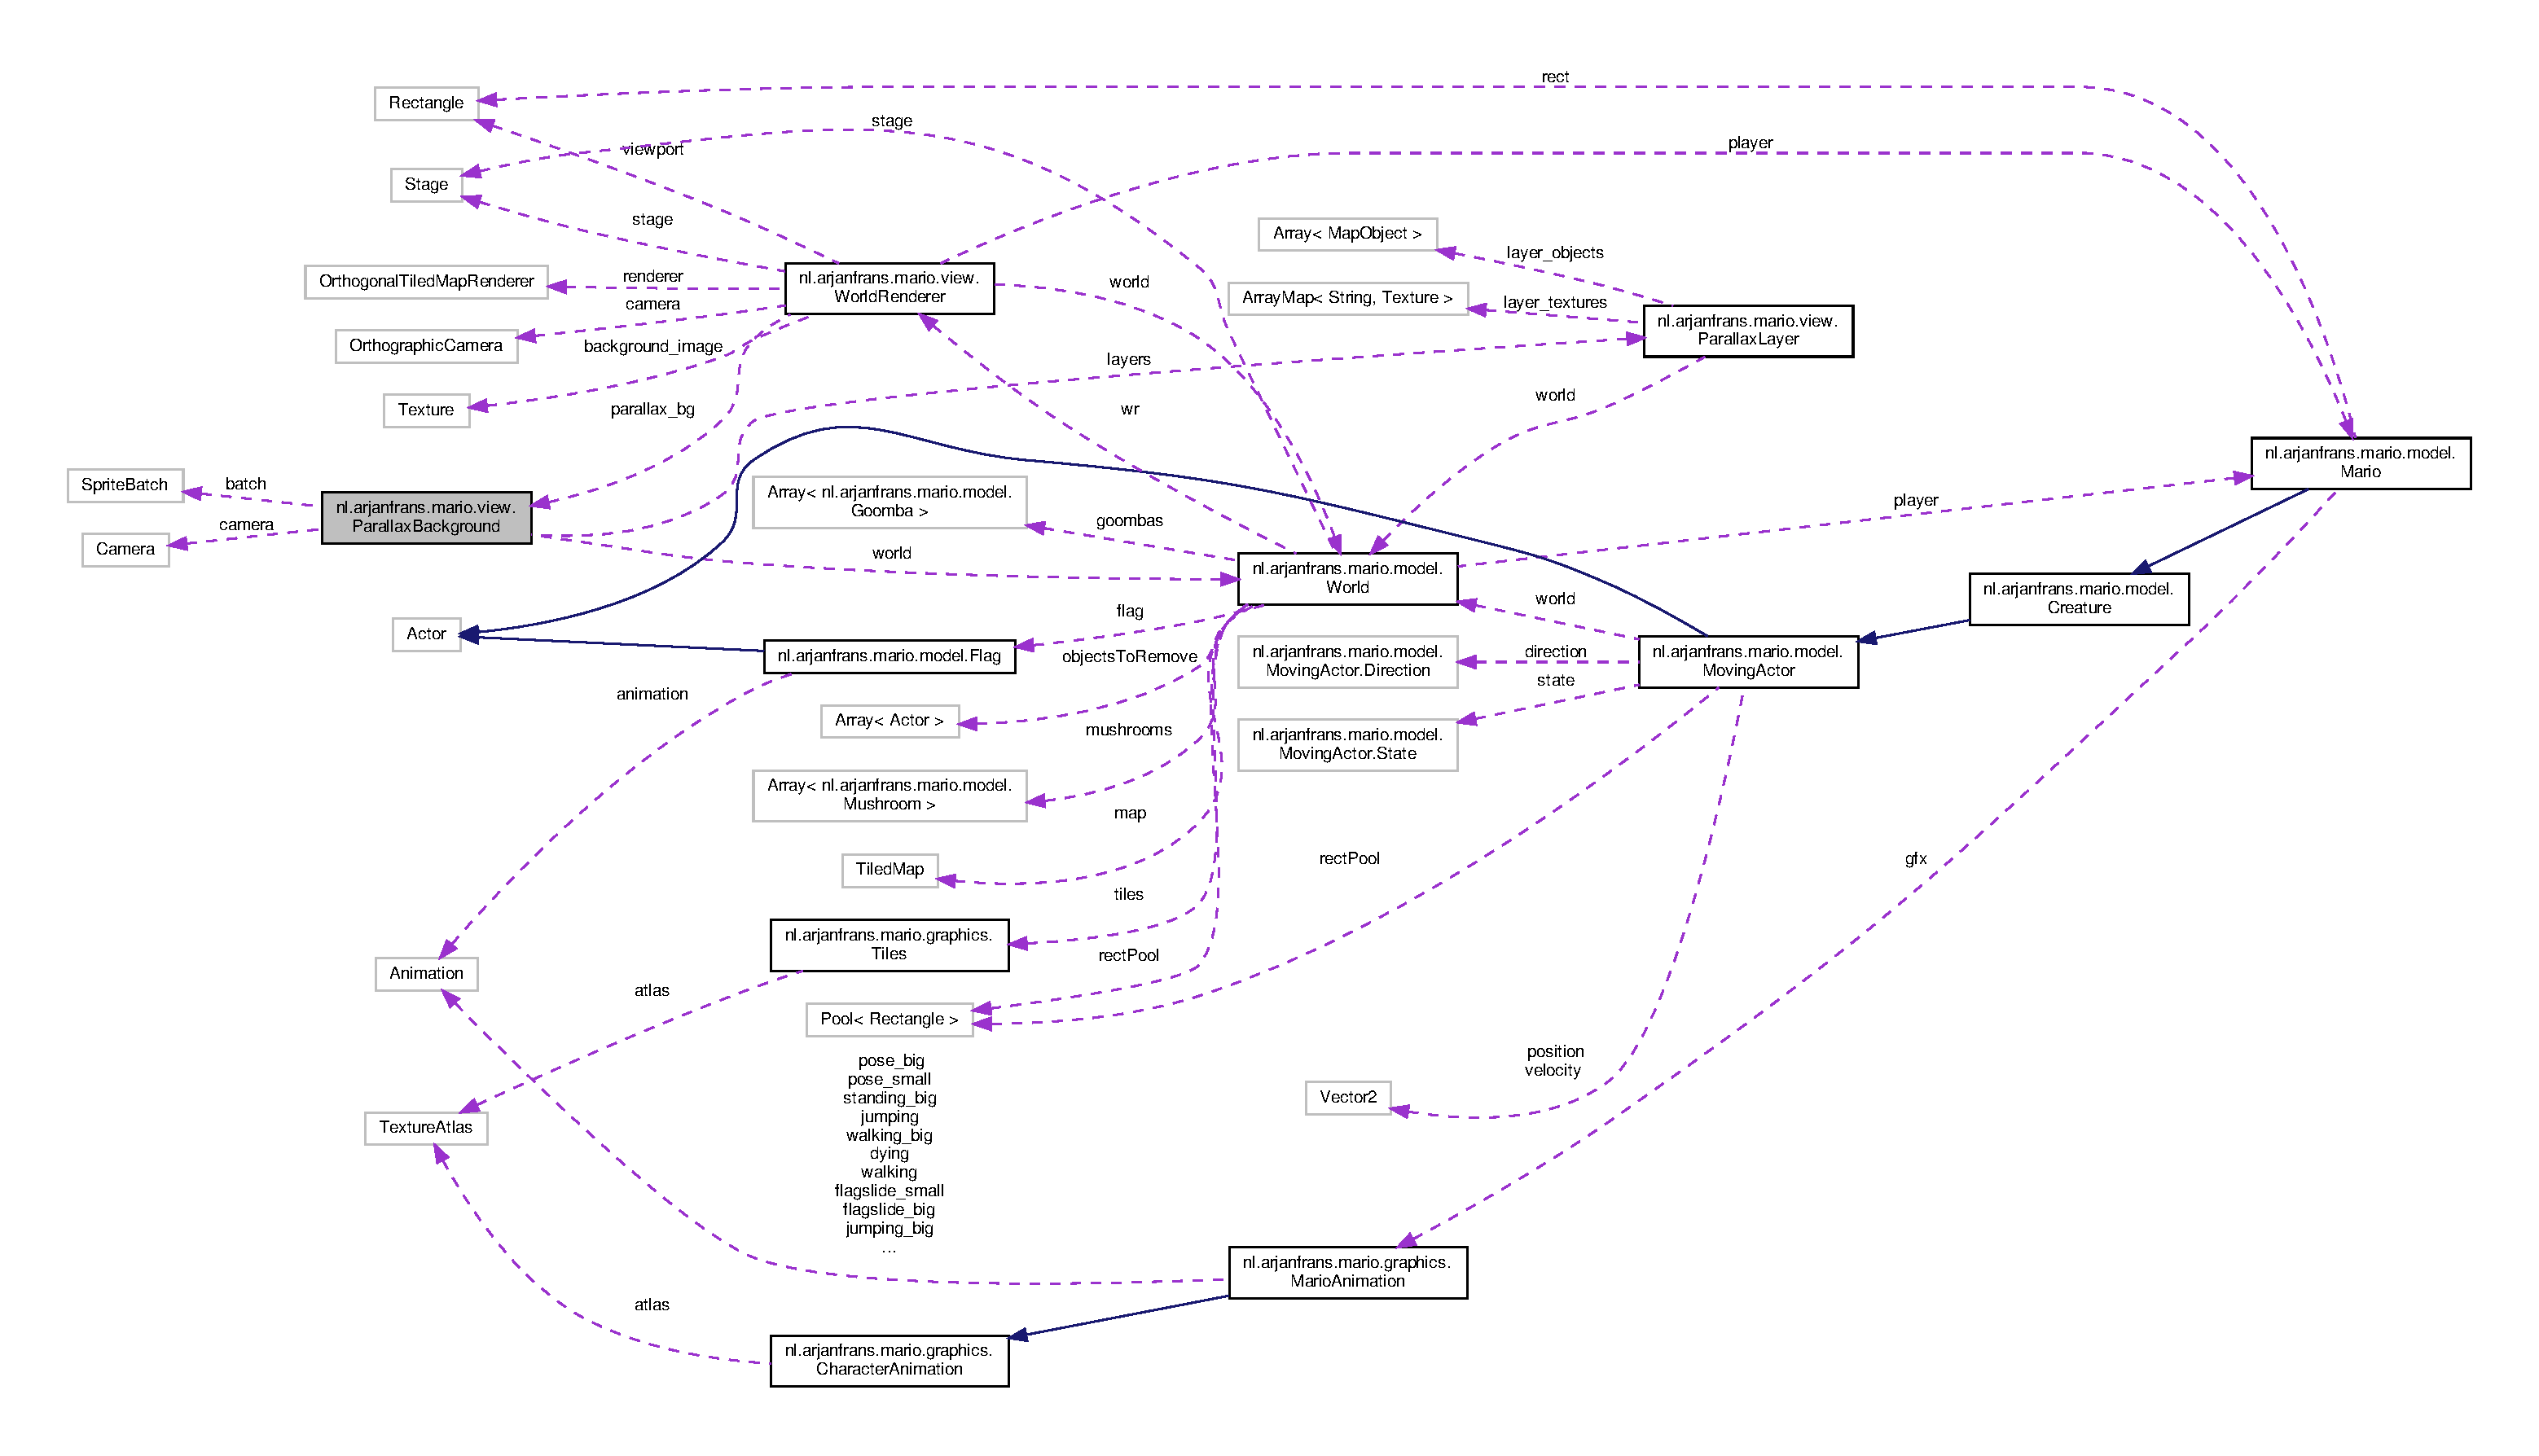
\includegraphics[width=350pt]{classnl_1_1arjanfrans_1_1mario_1_1view_1_1ParallaxBackground__coll__graph}
\end{center}
\end{figure}
\subsection*{Public Member Functions}
\begin{DoxyCompactItemize}
\item 
\hyperlink{classnl_1_1arjanfrans_1_1mario_1_1view_1_1ParallaxBackground_ad010a277850f31090a024be8da54e3bb}{Parallax\+Background} (\hyperlink{classnl_1_1arjanfrans_1_1mario_1_1model_1_1World}{World} world, \hyperlink{classnl_1_1arjanfrans_1_1mario_1_1view_1_1ParallaxLayer}{Parallax\+Layer}\mbox{[}$\,$\mbox{]} p\+Layers, Camera p\+Camera, Sprite\+Batch p\+Batch)
\begin{DoxyCompactList}\small\item\em Constructor method for \hyperlink{classnl_1_1arjanfrans_1_1mario_1_1view_1_1ParallaxBackground}{Parallax\+Background}. \end{DoxyCompactList}\item 
\mbox{\Hypertarget{classnl_1_1arjanfrans_1_1mario_1_1view_1_1ParallaxBackground_ac24d0a672fd58eaf3db65d09971c5f8a}\label{classnl_1_1arjanfrans_1_1mario_1_1view_1_1ParallaxBackground_ac24d0a672fd58eaf3db65d09971c5f8a}} 
void \hyperlink{classnl_1_1arjanfrans_1_1mario_1_1view_1_1ParallaxBackground_ac24d0a672fd58eaf3db65d09971c5f8a}{render} ()
\begin{DoxyCompactList}\small\item\em A method meant to render the parallax background. \end{DoxyCompactList}\item 
void \hyperlink{classnl_1_1arjanfrans_1_1mario_1_1view_1_1ParallaxBackground_af5959c6214b1e4fecd434a8022baf449}{moveX} (float p\+Delta)
\begin{DoxyCompactList}\small\item\em A method meant to move the parallax background on the x-\/axis. \end{DoxyCompactList}\item 
void \hyperlink{classnl_1_1arjanfrans_1_1mario_1_1view_1_1ParallaxBackground_a626301d2f854e2876a93f0df64e4b533}{moveY} (float p\+Delta)
\begin{DoxyCompactList}\small\item\em A method meant to move the parallax background on the y-\/axis. \end{DoxyCompactList}\item 
\mbox{\Hypertarget{classnl_1_1arjanfrans_1_1mario_1_1view_1_1ParallaxBackground_a4fb35c31a1d177b1105dbad0395867aa}\label{classnl_1_1arjanfrans_1_1mario_1_1view_1_1ParallaxBackground_a4fb35c31a1d177b1105dbad0395867aa}} 
void \hyperlink{classnl_1_1arjanfrans_1_1mario_1_1view_1_1ParallaxBackground_a4fb35c31a1d177b1105dbad0395867aa}{dispose} ()
\begin{DoxyCompactList}\small\item\em A method meant to dispose of all layers of the \hyperlink{classnl_1_1arjanfrans_1_1mario_1_1view_1_1ParallaxBackground}{Parallax\+Background}. \end{DoxyCompactList}\end{DoxyCompactItemize}
\subsection*{Private Member Functions}
\begin{DoxyCompactItemize}
\item 
void \hyperlink{classnl_1_1arjanfrans_1_1mario_1_1view_1_1ParallaxBackground_a1be3d3c6f4d8e0e74f3cae3cc77bd86a}{draw\+Layer} (\hyperlink{classnl_1_1arjanfrans_1_1mario_1_1view_1_1ParallaxLayer}{Parallax\+Layer} layer, Sprite\+Batch batch)
\begin{DoxyCompactList}\small\item\em A method meant to draw the layers of the Parallax background. \end{DoxyCompactList}\end{DoxyCompactItemize}
\subsection*{Private Attributes}
\begin{DoxyCompactItemize}
\item 
\mbox{\Hypertarget{classnl_1_1arjanfrans_1_1mario_1_1view_1_1ParallaxBackground_a211e859b253400b48342c39b2ee5bc83}\label{classnl_1_1arjanfrans_1_1mario_1_1view_1_1ParallaxBackground_a211e859b253400b48342c39b2ee5bc83}} 
\hyperlink{classnl_1_1arjanfrans_1_1mario_1_1view_1_1ParallaxLayer}{Parallax\+Layer} \mbox{[}$\,$\mbox{]} {\bfseries layers}
\item 
\mbox{\Hypertarget{classnl_1_1arjanfrans_1_1mario_1_1view_1_1ParallaxBackground_ab5f4b2babf8d021339dc9d3071910963}\label{classnl_1_1arjanfrans_1_1mario_1_1view_1_1ParallaxBackground_ab5f4b2babf8d021339dc9d3071910963}} 
Camera {\bfseries camera}
\item 
\mbox{\Hypertarget{classnl_1_1arjanfrans_1_1mario_1_1view_1_1ParallaxBackground_acf3064f2616488f3faafe0f524490b15}\label{classnl_1_1arjanfrans_1_1mario_1_1view_1_1ParallaxBackground_acf3064f2616488f3faafe0f524490b15}} 
Sprite\+Batch {\bfseries batch}
\item 
\mbox{\Hypertarget{classnl_1_1arjanfrans_1_1mario_1_1view_1_1ParallaxBackground_a5e17b02daeb130aa81b146d417d0a86f}\label{classnl_1_1arjanfrans_1_1mario_1_1view_1_1ParallaxBackground_a5e17b02daeb130aa81b146d417d0a86f}} 
\hyperlink{classnl_1_1arjanfrans_1_1mario_1_1model_1_1World}{World} {\bfseries world}
\end{DoxyCompactItemize}


\subsection{Detailed Description}
The class meant to create a parallax background. 

\subsection{Constructor \& Destructor Documentation}
\mbox{\Hypertarget{classnl_1_1arjanfrans_1_1mario_1_1view_1_1ParallaxBackground_ad010a277850f31090a024be8da54e3bb}\label{classnl_1_1arjanfrans_1_1mario_1_1view_1_1ParallaxBackground_ad010a277850f31090a024be8da54e3bb}} 
\index{nl\+::arjanfrans\+::mario\+::view\+::\+Parallax\+Background@{nl\+::arjanfrans\+::mario\+::view\+::\+Parallax\+Background}!Parallax\+Background@{Parallax\+Background}}
\index{Parallax\+Background@{Parallax\+Background}!nl\+::arjanfrans\+::mario\+::view\+::\+Parallax\+Background@{nl\+::arjanfrans\+::mario\+::view\+::\+Parallax\+Background}}
\subsubsection{\texorpdfstring{Parallax\+Background()}{ParallaxBackground()}}
{\footnotesize\ttfamily nl.\+arjanfrans.\+mario.\+view.\+Parallax\+Background.\+Parallax\+Background (\begin{DoxyParamCaption}\item[{\hyperlink{classnl_1_1arjanfrans_1_1mario_1_1model_1_1World}{World}}]{world,  }\item[{\hyperlink{classnl_1_1arjanfrans_1_1mario_1_1view_1_1ParallaxLayer}{Parallax\+Layer} \mbox{[}$\,$\mbox{]}}]{p\+Layers,  }\item[{Camera}]{p\+Camera,  }\item[{Sprite\+Batch}]{p\+Batch }\end{DoxyParamCaption})}



Constructor method for \hyperlink{classnl_1_1arjanfrans_1_1mario_1_1view_1_1ParallaxBackground}{Parallax\+Background}. 


\begin{DoxyParams}{Parameters}
{\em world} & -\/ the world that the \hyperlink{classnl_1_1arjanfrans_1_1mario_1_1view_1_1ParallaxBackground}{Parallax\+Background} is displaying \\
\hline
{\em p\+Layers} & -\/ an array of Parallax\+Layers \\
\hline
{\em p\+Camera} & -\/ a Camera object that will move back and forth on the background \\
\hline
{\em p\+Batch} & -\/ a Sprite\+Batch object \\
\hline
\end{DoxyParams}
\begin{DoxyReturn}{Returns}
an instance of \hyperlink{classnl_1_1arjanfrans_1_1mario_1_1view_1_1ParallaxBackground}{Parallax\+Background} 
\end{DoxyReturn}


\subsection{Member Function Documentation}
\mbox{\Hypertarget{classnl_1_1arjanfrans_1_1mario_1_1view_1_1ParallaxBackground_a1be3d3c6f4d8e0e74f3cae3cc77bd86a}\label{classnl_1_1arjanfrans_1_1mario_1_1view_1_1ParallaxBackground_a1be3d3c6f4d8e0e74f3cae3cc77bd86a}} 
\index{nl\+::arjanfrans\+::mario\+::view\+::\+Parallax\+Background@{nl\+::arjanfrans\+::mario\+::view\+::\+Parallax\+Background}!draw\+Layer@{draw\+Layer}}
\index{draw\+Layer@{draw\+Layer}!nl\+::arjanfrans\+::mario\+::view\+::\+Parallax\+Background@{nl\+::arjanfrans\+::mario\+::view\+::\+Parallax\+Background}}
\subsubsection{\texorpdfstring{draw\+Layer()}{drawLayer()}}
{\footnotesize\ttfamily void nl.\+arjanfrans.\+mario.\+view.\+Parallax\+Background.\+draw\+Layer (\begin{DoxyParamCaption}\item[{\hyperlink{classnl_1_1arjanfrans_1_1mario_1_1view_1_1ParallaxLayer}{Parallax\+Layer}}]{layer,  }\item[{Sprite\+Batch}]{batch }\end{DoxyParamCaption})\hspace{0.3cm}{\ttfamily [private]}}



A method meant to draw the layers of the Parallax background. 


\begin{DoxyParams}{Parameters}
{\em layer} & -\/ a \hyperlink{classnl_1_1arjanfrans_1_1mario_1_1view_1_1ParallaxLayer}{Parallax\+Layer} \\
\hline
{\em batch} & -\/ a Sprite\+Batch object \\
\hline
\end{DoxyParams}
\mbox{\Hypertarget{classnl_1_1arjanfrans_1_1mario_1_1view_1_1ParallaxBackground_af5959c6214b1e4fecd434a8022baf449}\label{classnl_1_1arjanfrans_1_1mario_1_1view_1_1ParallaxBackground_af5959c6214b1e4fecd434a8022baf449}} 
\index{nl\+::arjanfrans\+::mario\+::view\+::\+Parallax\+Background@{nl\+::arjanfrans\+::mario\+::view\+::\+Parallax\+Background}!moveX@{moveX}}
\index{moveX@{moveX}!nl\+::arjanfrans\+::mario\+::view\+::\+Parallax\+Background@{nl\+::arjanfrans\+::mario\+::view\+::\+Parallax\+Background}}
\subsubsection{\texorpdfstring{move\+X()}{moveX()}}
{\footnotesize\ttfamily void nl.\+arjanfrans.\+mario.\+view.\+Parallax\+Background.\+moveX (\begin{DoxyParamCaption}\item[{float}]{p\+Delta }\end{DoxyParamCaption})}



A method meant to move the parallax background on the x-\/axis. 


\begin{DoxyParams}{Parameters}
{\em p\+Delta} & -\/ a float constant indicating how much to move by on the x -\/ axis \\
\hline
\end{DoxyParams}
\mbox{\Hypertarget{classnl_1_1arjanfrans_1_1mario_1_1view_1_1ParallaxBackground_a626301d2f854e2876a93f0df64e4b533}\label{classnl_1_1arjanfrans_1_1mario_1_1view_1_1ParallaxBackground_a626301d2f854e2876a93f0df64e4b533}} 
\index{nl\+::arjanfrans\+::mario\+::view\+::\+Parallax\+Background@{nl\+::arjanfrans\+::mario\+::view\+::\+Parallax\+Background}!moveY@{moveY}}
\index{moveY@{moveY}!nl\+::arjanfrans\+::mario\+::view\+::\+Parallax\+Background@{nl\+::arjanfrans\+::mario\+::view\+::\+Parallax\+Background}}
\subsubsection{\texorpdfstring{move\+Y()}{moveY()}}
{\footnotesize\ttfamily void nl.\+arjanfrans.\+mario.\+view.\+Parallax\+Background.\+moveY (\begin{DoxyParamCaption}\item[{float}]{p\+Delta }\end{DoxyParamCaption})}



A method meant to move the parallax background on the y-\/axis. 


\begin{DoxyParams}{Parameters}
{\em p\+Delta} & -\/ a float constant indicating how much to move by on the y -\/ axis \\
\hline
\end{DoxyParams}


The documentation for this class was generated from the following file\+:\begin{DoxyCompactItemize}
\item 
core/src/nl/arjanfrans/mario/view/Parallax\+Background.\+java\end{DoxyCompactItemize}

\hypertarget{classnl_1_1arjanfrans_1_1mario_1_1view_1_1ParallaxLayer}{}\section{nl.\+arjanfrans.\+mario.\+view.\+Parallax\+Layer Class Reference}
\label{classnl_1_1arjanfrans_1_1mario_1_1view_1_1ParallaxLayer}\index{nl.\+arjanfrans.\+mario.\+view.\+Parallax\+Layer@{nl.\+arjanfrans.\+mario.\+view.\+Parallax\+Layer}}


The class meant to retrieve a layer from a \hyperlink{classnl_1_1arjanfrans_1_1mario_1_1view_1_1ParallaxBackground}{Parallax\+Background}.  




Collaboration diagram for nl.\+arjanfrans.\+mario.\+view.\+Parallax\+Layer\+:
\nopagebreak
\begin{figure}[H]
\begin{center}
\leavevmode
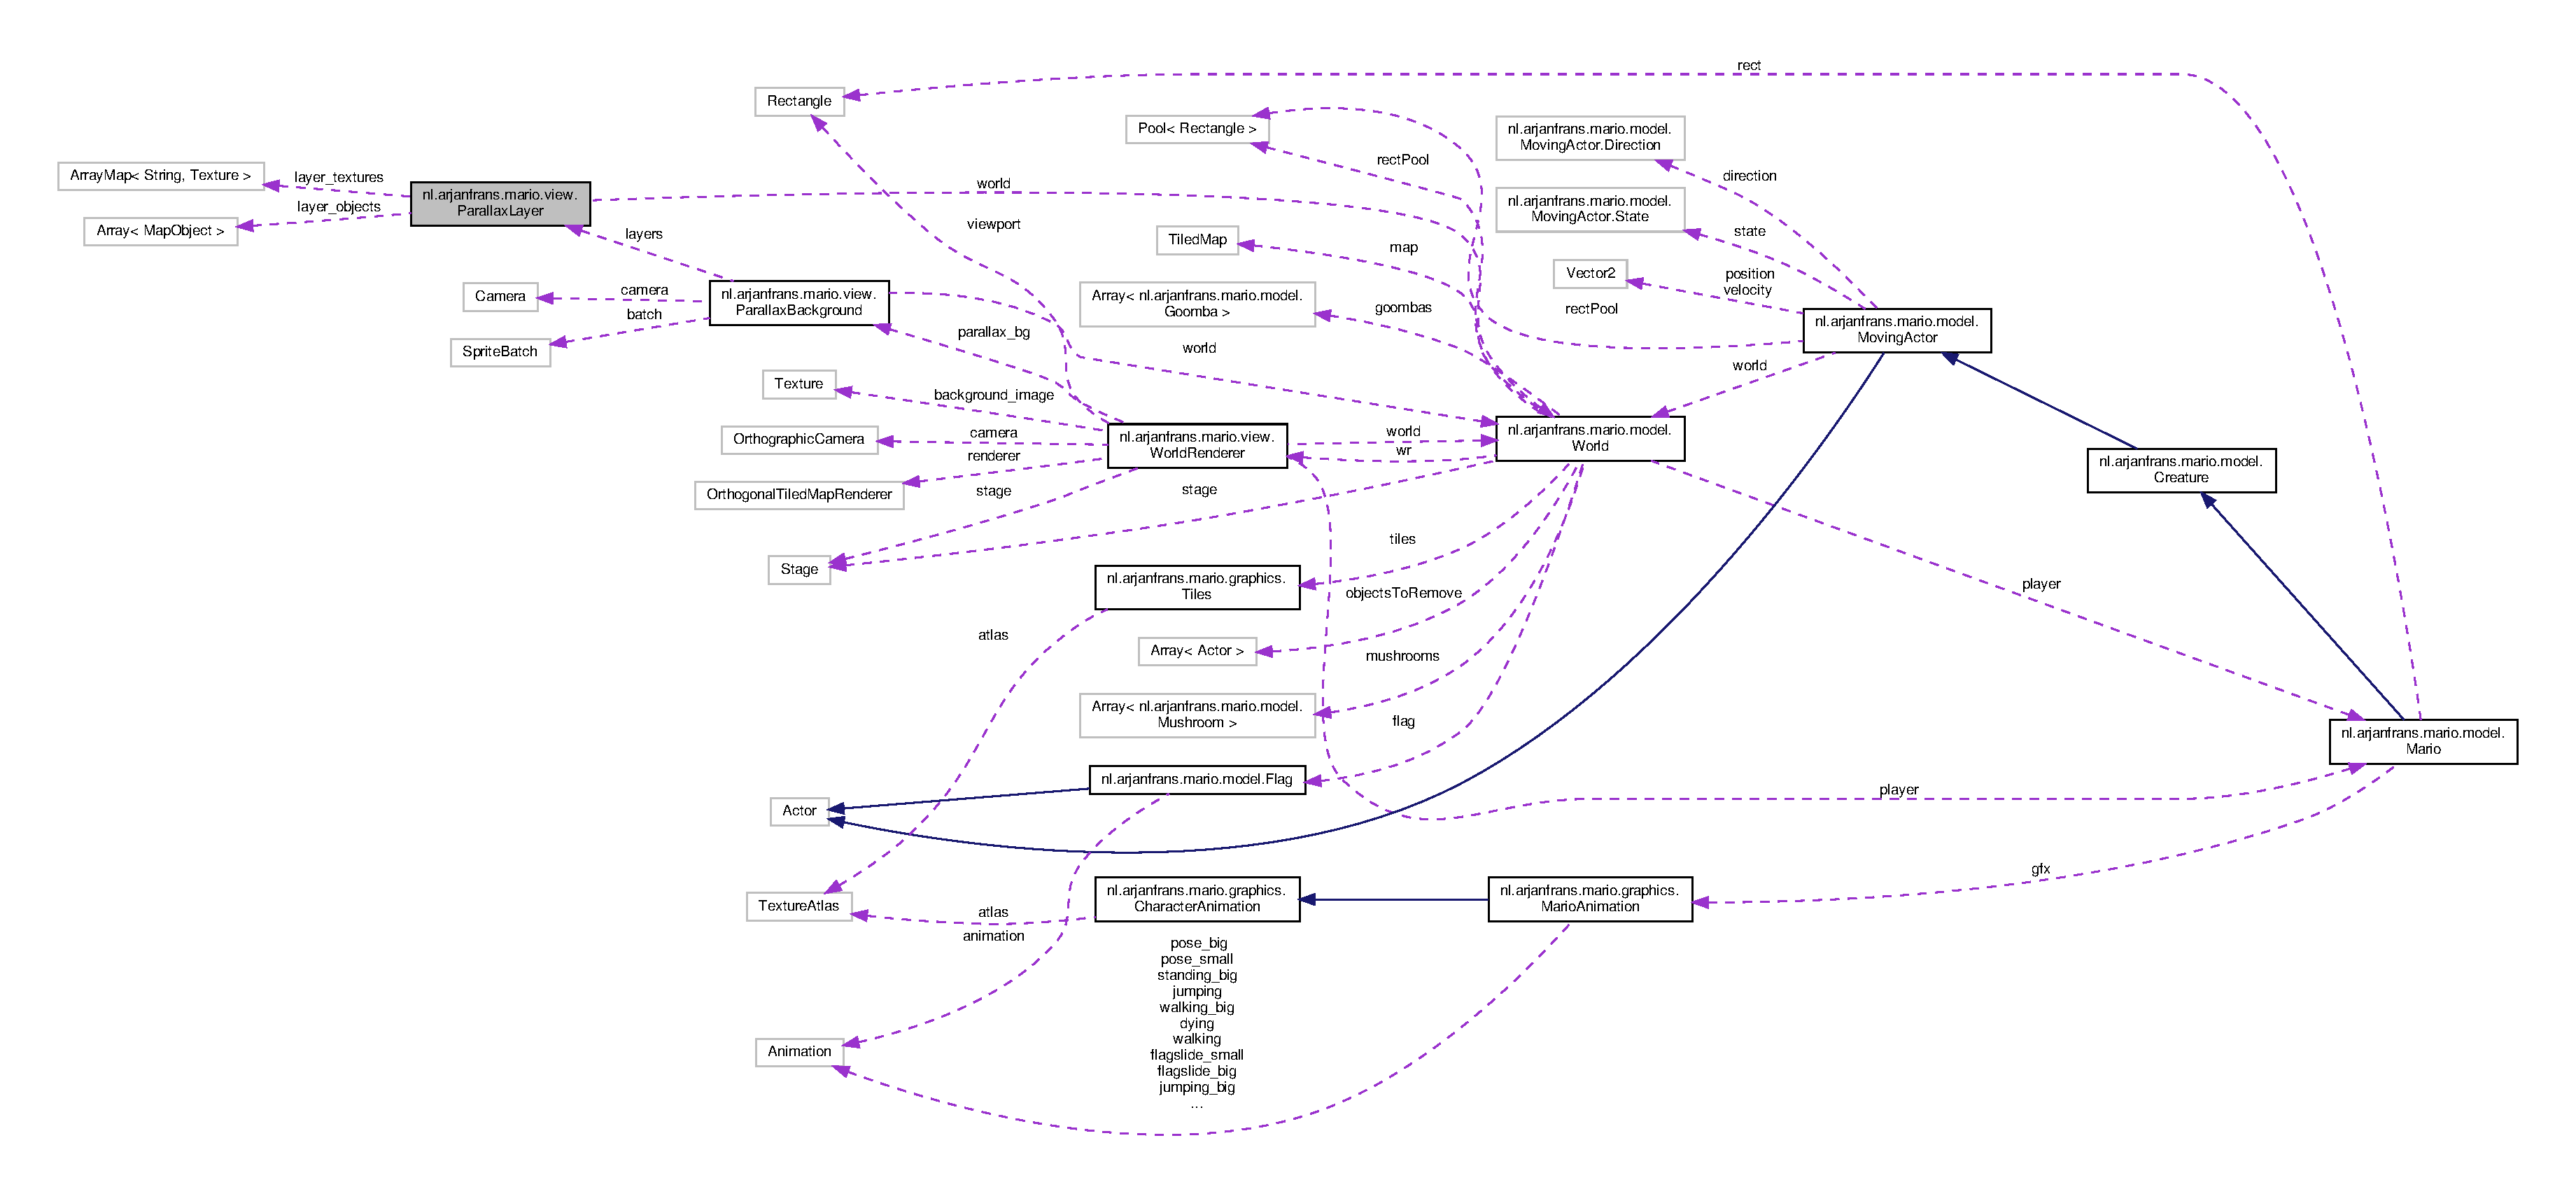
\includegraphics[width=350pt]{classnl_1_1arjanfrans_1_1mario_1_1view_1_1ParallaxLayer__coll__graph}
\end{center}
\end{figure}
\subsection*{Public Member Functions}
\begin{DoxyCompactItemize}
\item 
\hyperlink{classnl_1_1arjanfrans_1_1mario_1_1view_1_1ParallaxLayer_aec238fa2067afb4e286f8db8b616aeac}{Parallax\+Layer} (\hyperlink{classnl_1_1arjanfrans_1_1mario_1_1model_1_1World}{World} world, String layer\+\_\+name, float p\+RatioX, float p\+RatioY)
\begin{DoxyCompactList}\small\item\em Constructor method for \hyperlink{classnl_1_1arjanfrans_1_1mario_1_1view_1_1ParallaxLayer}{Parallax\+Layer}. \end{DoxyCompactList}\item 
\mbox{\Hypertarget{classnl_1_1arjanfrans_1_1mario_1_1view_1_1ParallaxLayer_a1d299e94c27d8fd0b37d37110f52ff60}\label{classnl_1_1arjanfrans_1_1mario_1_1view_1_1ParallaxLayer_a1d299e94c27d8fd0b37d37110f52ff60}} 
Array\+Map$<$ String, Texture $>$ {\bfseries get\+Layer\+Textures} ()
\item 
\mbox{\Hypertarget{classnl_1_1arjanfrans_1_1mario_1_1view_1_1ParallaxLayer_ad211dbd4512b3560a25c2d09f95fa260}\label{classnl_1_1arjanfrans_1_1mario_1_1view_1_1ParallaxLayer_ad211dbd4512b3560a25c2d09f95fa260}} 
Array$<$ Map\+Object $>$ {\bfseries get\+Layer\+Objects} ()
\item 
\mbox{\Hypertarget{classnl_1_1arjanfrans_1_1mario_1_1view_1_1ParallaxLayer_a0d7584aed429cdc488e32ec4eae94df1}\label{classnl_1_1arjanfrans_1_1mario_1_1view_1_1ParallaxLayer_a0d7584aed429cdc488e32ec4eae94df1}} 
void \hyperlink{classnl_1_1arjanfrans_1_1mario_1_1view_1_1ParallaxLayer_a0d7584aed429cdc488e32ec4eae94df1}{dispose} ()
\begin{DoxyCompactList}\small\item\em A method meant to dispose of all layer textures of the \hyperlink{classnl_1_1arjanfrans_1_1mario_1_1view_1_1ParallaxLayer}{Parallax\+Layer}. \end{DoxyCompactList}\end{DoxyCompactItemize}
\subsection*{Protected Member Functions}
\begin{DoxyCompactItemize}
\item 
void \hyperlink{classnl_1_1arjanfrans_1_1mario_1_1view_1_1ParallaxLayer_a12e98853c0a5eaadc896bc50c8bd84dc}{moveX} (float p\+Delta)
\begin{DoxyCompactList}\small\item\em A method meant to move this layer in the x direction, based on a constant value. \end{DoxyCompactList}\item 
void \hyperlink{classnl_1_1arjanfrans_1_1mario_1_1view_1_1ParallaxLayer_a961341849470a053f57c1a08000cdf69}{moveY} (float p\+Delta)
\begin{DoxyCompactList}\small\item\em A method meant to move this layer in the y direction, based on a constant value. \end{DoxyCompactList}\end{DoxyCompactItemize}
\subsection*{Private Member Functions}
\begin{DoxyCompactItemize}
\item 
\mbox{\Hypertarget{classnl_1_1arjanfrans_1_1mario_1_1view_1_1ParallaxLayer_afbeccae3b9bf53a6ae696b185100e0b8}\label{classnl_1_1arjanfrans_1_1mario_1_1view_1_1ParallaxLayer_afbeccae3b9bf53a6ae696b185100e0b8}} 
void \hyperlink{classnl_1_1arjanfrans_1_1mario_1_1view_1_1ParallaxLayer_afbeccae3b9bf53a6ae696b185100e0b8}{load\+Objects} ()
\begin{DoxyCompactList}\small\item\em A method meant to load the objects from the tmx file, convert them into textures and put them on the layer. \end{DoxyCompactList}\end{DoxyCompactItemize}
\subsection*{Private Attributes}
\begin{DoxyCompactItemize}
\item 
\mbox{\Hypertarget{classnl_1_1arjanfrans_1_1mario_1_1view_1_1ParallaxLayer_ab8a033d010684f7e59398046887ca726}\label{classnl_1_1arjanfrans_1_1mario_1_1view_1_1ParallaxLayer_ab8a033d010684f7e59398046887ca726}} 
\hyperlink{classnl_1_1arjanfrans_1_1mario_1_1model_1_1World}{World} {\bfseries world}
\item 
\mbox{\Hypertarget{classnl_1_1arjanfrans_1_1mario_1_1view_1_1ParallaxLayer_a8199fd99969e10e6339ac95896c44e77}\label{classnl_1_1arjanfrans_1_1mario_1_1view_1_1ParallaxLayer_a8199fd99969e10e6339ac95896c44e77}} 
Array$<$ Map\+Object $>$ {\bfseries layer\+\_\+objects}
\item 
\mbox{\Hypertarget{classnl_1_1arjanfrans_1_1mario_1_1view_1_1ParallaxLayer_a738382929b532aa9d8aeb39b70b3e3a6}\label{classnl_1_1arjanfrans_1_1mario_1_1view_1_1ParallaxLayer_a738382929b532aa9d8aeb39b70b3e3a6}} 
Array\+Map$<$ String, Texture $>$ {\bfseries layer\+\_\+textures}
\item 
\mbox{\Hypertarget{classnl_1_1arjanfrans_1_1mario_1_1view_1_1ParallaxLayer_acb8fb1a4b8028154adc4622df84bf552}\label{classnl_1_1arjanfrans_1_1mario_1_1view_1_1ParallaxLayer_acb8fb1a4b8028154adc4622df84bf552}} 
String {\bfseries layer\+\_\+name}
\end{DoxyCompactItemize}


\subsection{Detailed Description}
The class meant to retrieve a layer from a \hyperlink{classnl_1_1arjanfrans_1_1mario_1_1view_1_1ParallaxBackground}{Parallax\+Background}. 

\subsection{Constructor \& Destructor Documentation}
\mbox{\Hypertarget{classnl_1_1arjanfrans_1_1mario_1_1view_1_1ParallaxLayer_aec238fa2067afb4e286f8db8b616aeac}\label{classnl_1_1arjanfrans_1_1mario_1_1view_1_1ParallaxLayer_aec238fa2067afb4e286f8db8b616aeac}} 
\index{nl\+::arjanfrans\+::mario\+::view\+::\+Parallax\+Layer@{nl\+::arjanfrans\+::mario\+::view\+::\+Parallax\+Layer}!Parallax\+Layer@{Parallax\+Layer}}
\index{Parallax\+Layer@{Parallax\+Layer}!nl\+::arjanfrans\+::mario\+::view\+::\+Parallax\+Layer@{nl\+::arjanfrans\+::mario\+::view\+::\+Parallax\+Layer}}
\subsubsection{\texorpdfstring{Parallax\+Layer()}{ParallaxLayer()}}
{\footnotesize\ttfamily nl.\+arjanfrans.\+mario.\+view.\+Parallax\+Layer.\+Parallax\+Layer (\begin{DoxyParamCaption}\item[{\hyperlink{classnl_1_1arjanfrans_1_1mario_1_1model_1_1World}{World}}]{world,  }\item[{String}]{layer\+\_\+name,  }\item[{float}]{p\+RatioX,  }\item[{float}]{p\+RatioY }\end{DoxyParamCaption})}



Constructor method for \hyperlink{classnl_1_1arjanfrans_1_1mario_1_1view_1_1ParallaxLayer}{Parallax\+Layer}. 


\begin{DoxyParams}{Parameters}
{\em world} & -\/ The world that the \hyperlink{classnl_1_1arjanfrans_1_1mario_1_1view_1_1ParallaxLayer}{Parallax\+Layer} exists in \\
\hline
{\em layer\+\_\+name} & -\/ a string representing the name of the layer \\
\hline
{\em p\+RatioX} & -\/ a float representing how much the layer will move in the x direction if the background is moved. \\
\hline
{\em p\+RatioY} & -\/ a float representing how much the layer will move in the y direction if the background is moved. \\
\hline
\end{DoxyParams}


\subsection{Member Function Documentation}
\mbox{\Hypertarget{classnl_1_1arjanfrans_1_1mario_1_1view_1_1ParallaxLayer_a12e98853c0a5eaadc896bc50c8bd84dc}\label{classnl_1_1arjanfrans_1_1mario_1_1view_1_1ParallaxLayer_a12e98853c0a5eaadc896bc50c8bd84dc}} 
\index{nl\+::arjanfrans\+::mario\+::view\+::\+Parallax\+Layer@{nl\+::arjanfrans\+::mario\+::view\+::\+Parallax\+Layer}!moveX@{moveX}}
\index{moveX@{moveX}!nl\+::arjanfrans\+::mario\+::view\+::\+Parallax\+Layer@{nl\+::arjanfrans\+::mario\+::view\+::\+Parallax\+Layer}}
\subsubsection{\texorpdfstring{move\+X()}{moveX()}}
{\footnotesize\ttfamily void nl.\+arjanfrans.\+mario.\+view.\+Parallax\+Layer.\+moveX (\begin{DoxyParamCaption}\item[{float}]{p\+Delta }\end{DoxyParamCaption})\hspace{0.3cm}{\ttfamily [protected]}}



A method meant to move this layer in the x direction, based on a constant value. 


\begin{DoxyParams}{Parameters}
{\em p\+Delta} & -\/ a float representing the shift in the layer. \\
\hline
\end{DoxyParams}
\mbox{\Hypertarget{classnl_1_1arjanfrans_1_1mario_1_1view_1_1ParallaxLayer_a961341849470a053f57c1a08000cdf69}\label{classnl_1_1arjanfrans_1_1mario_1_1view_1_1ParallaxLayer_a961341849470a053f57c1a08000cdf69}} 
\index{nl\+::arjanfrans\+::mario\+::view\+::\+Parallax\+Layer@{nl\+::arjanfrans\+::mario\+::view\+::\+Parallax\+Layer}!moveY@{moveY}}
\index{moveY@{moveY}!nl\+::arjanfrans\+::mario\+::view\+::\+Parallax\+Layer@{nl\+::arjanfrans\+::mario\+::view\+::\+Parallax\+Layer}}
\subsubsection{\texorpdfstring{move\+Y()}{moveY()}}
{\footnotesize\ttfamily void nl.\+arjanfrans.\+mario.\+view.\+Parallax\+Layer.\+moveY (\begin{DoxyParamCaption}\item[{float}]{p\+Delta }\end{DoxyParamCaption})\hspace{0.3cm}{\ttfamily [protected]}}



A method meant to move this layer in the y direction, based on a constant value. 


\begin{DoxyParams}{Parameters}
{\em p\+Delta} & -\/ a float representing the shift in the layer. \\
\hline
\end{DoxyParams}


The documentation for this class was generated from the following file\+:\begin{DoxyCompactItemize}
\item 
core/src/nl/arjanfrans/mario/view/Parallax\+Layer.\+java\end{DoxyCompactItemize}

\hypertarget{classnl_1_1arjanfrans_1_1mario_1_1model_1_1StaticActor}{}\section{nl.\+arjanfrans.\+mario.\+model.\+Static\+Actor Class Reference}
\label{classnl_1_1arjanfrans_1_1mario_1_1model_1_1StaticActor}\index{nl.\+arjanfrans.\+mario.\+model.\+Static\+Actor@{nl.\+arjanfrans.\+mario.\+model.\+Static\+Actor}}


Inherited class that represents static actor.  




Inheritance diagram for nl.\+arjanfrans.\+mario.\+model.\+Static\+Actor\+:
\nopagebreak
\begin{figure}[H]
\begin{center}
\leavevmode
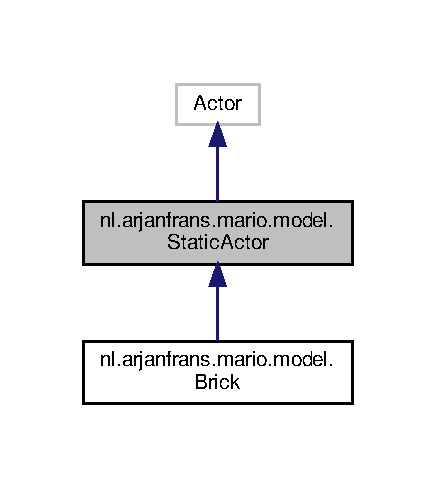
\includegraphics[width=209pt]{classnl_1_1arjanfrans_1_1mario_1_1model_1_1StaticActor__inherit__graph}
\end{center}
\end{figure}


Collaboration diagram for nl.\+arjanfrans.\+mario.\+model.\+Static\+Actor\+:
\nopagebreak
\begin{figure}[H]
\begin{center}
\leavevmode
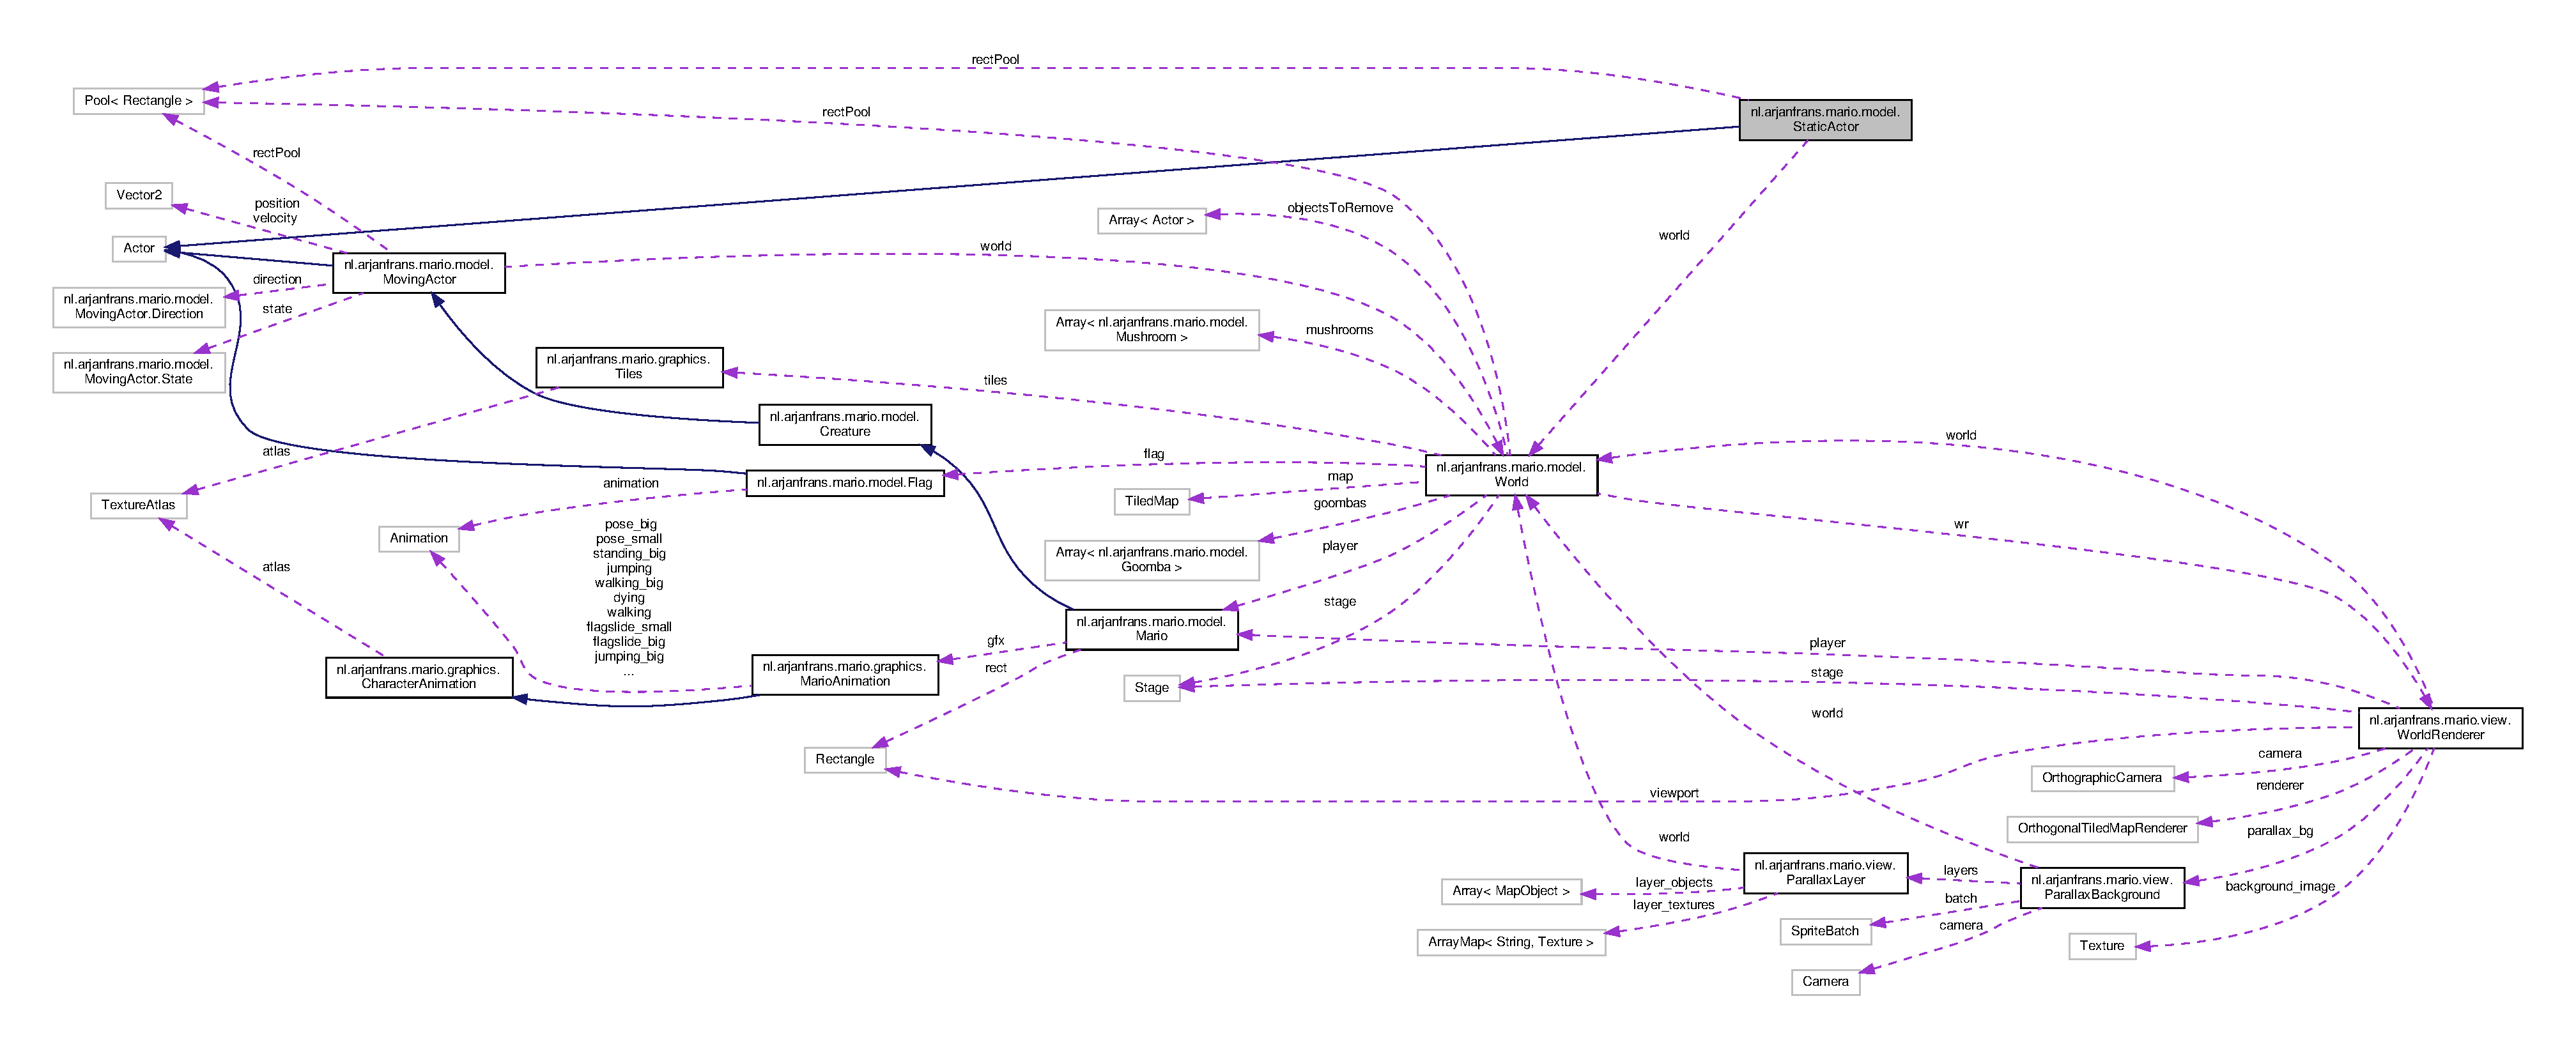
\includegraphics[width=350pt]{classnl_1_1arjanfrans_1_1mario_1_1model_1_1StaticActor__coll__graph}
\end{center}
\end{figure}
\subsection*{Public Member Functions}
\begin{DoxyCompactItemize}
\item 
\hyperlink{classnl_1_1arjanfrans_1_1mario_1_1model_1_1StaticActor_aa558f637b07d753909e51f5cebe6168c}{Static\+Actor} (\hyperlink{classnl_1_1arjanfrans_1_1mario_1_1model_1_1World}{World} world)
\begin{DoxyCompactList}\small\item\em Constructor method. \end{DoxyCompactList}\item 
Rectangle \hyperlink{classnl_1_1arjanfrans_1_1mario_1_1model_1_1StaticActor_a39be7695e6cb67d19267dd5c6ae5e264}{rectangle} ()
\begin{DoxyCompactList}\small\item\em Get object Rectangle. \end{DoxyCompactList}\item 
boolean \hyperlink{classnl_1_1arjanfrans_1_1mario_1_1model_1_1StaticActor_af44668107f69c1ec7547a7fb36537c43}{is\+Destroyed} ()
\begin{DoxyCompactList}\small\item\em Get boolean. \end{DoxyCompactList}\end{DoxyCompactItemize}
\subsection*{Protected Member Functions}
\begin{DoxyCompactItemize}
\item 
\mbox{\Hypertarget{classnl_1_1arjanfrans_1_1mario_1_1model_1_1StaticActor_a2cb4aa1c38965ace19ec77a38e599afc}\label{classnl_1_1arjanfrans_1_1mario_1_1model_1_1StaticActor_a2cb4aa1c38965ace19ec77a38e599afc}} 
abstract void {\bfseries hit} (int mario\+\_\+level)
\end{DoxyCompactItemize}
\subsection*{Protected Attributes}
\begin{DoxyCompactItemize}
\item 
\mbox{\Hypertarget{classnl_1_1arjanfrans_1_1mario_1_1model_1_1StaticActor_ae4707b92f60b23175bc3850faa27e7d6}\label{classnl_1_1arjanfrans_1_1mario_1_1model_1_1StaticActor_ae4707b92f60b23175bc3850faa27e7d6}} 
\hyperlink{classnl_1_1arjanfrans_1_1mario_1_1model_1_1World}{World} {\bfseries world}
\item 
\mbox{\Hypertarget{classnl_1_1arjanfrans_1_1mario_1_1model_1_1StaticActor_a0b8cdccbd26a618eab8963d47397c607}\label{classnl_1_1arjanfrans_1_1mario_1_1model_1_1StaticActor_a0b8cdccbd26a618eab8963d47397c607}} 
boolean {\bfseries destroyed}
\item 
Pool$<$ Rectangle $>$ {\bfseries rect\+Pool}
\end{DoxyCompactItemize}


\subsection{Detailed Description}
Inherited class that represents static actor. 

\subsection{Constructor \& Destructor Documentation}
\mbox{\Hypertarget{classnl_1_1arjanfrans_1_1mario_1_1model_1_1StaticActor_aa558f637b07d753909e51f5cebe6168c}\label{classnl_1_1arjanfrans_1_1mario_1_1model_1_1StaticActor_aa558f637b07d753909e51f5cebe6168c}} 
\index{nl\+::arjanfrans\+::mario\+::model\+::\+Static\+Actor@{nl\+::arjanfrans\+::mario\+::model\+::\+Static\+Actor}!Static\+Actor@{Static\+Actor}}
\index{Static\+Actor@{Static\+Actor}!nl\+::arjanfrans\+::mario\+::model\+::\+Static\+Actor@{nl\+::arjanfrans\+::mario\+::model\+::\+Static\+Actor}}
\subsubsection{\texorpdfstring{Static\+Actor()}{StaticActor()}}
{\footnotesize\ttfamily nl.\+arjanfrans.\+mario.\+model.\+Static\+Actor.\+Static\+Actor (\begin{DoxyParamCaption}\item[{\hyperlink{classnl_1_1arjanfrans_1_1mario_1_1model_1_1World}{World}}]{world }\end{DoxyParamCaption})}



Constructor method. 

Method which initializes an instance of \hyperlink{classnl_1_1arjanfrans_1_1mario_1_1model_1_1StaticActor}{Static\+Actor} 
\begin{DoxyParams}{Parameters}
{\em world} & The world object in which \hyperlink{classnl_1_1arjanfrans_1_1mario_1_1model_1_1Mario}{Mario} will exist in \\
\hline
\end{DoxyParams}


\subsection{Member Function Documentation}
\mbox{\Hypertarget{classnl_1_1arjanfrans_1_1mario_1_1model_1_1StaticActor_af44668107f69c1ec7547a7fb36537c43}\label{classnl_1_1arjanfrans_1_1mario_1_1model_1_1StaticActor_af44668107f69c1ec7547a7fb36537c43}} 
\index{nl\+::arjanfrans\+::mario\+::model\+::\+Static\+Actor@{nl\+::arjanfrans\+::mario\+::model\+::\+Static\+Actor}!is\+Destroyed@{is\+Destroyed}}
\index{is\+Destroyed@{is\+Destroyed}!nl\+::arjanfrans\+::mario\+::model\+::\+Static\+Actor@{nl\+::arjanfrans\+::mario\+::model\+::\+Static\+Actor}}
\subsubsection{\texorpdfstring{is\+Destroyed()}{isDestroyed()}}
{\footnotesize\ttfamily boolean nl.\+arjanfrans.\+mario.\+model.\+Static\+Actor.\+is\+Destroyed (\begin{DoxyParamCaption}{ }\end{DoxyParamCaption})}



Get boolean. 

\begin{DoxyReturn}{Returns}
destroyed boolean value true if destroyed 
\end{DoxyReturn}
\mbox{\Hypertarget{classnl_1_1arjanfrans_1_1mario_1_1model_1_1StaticActor_a39be7695e6cb67d19267dd5c6ae5e264}\label{classnl_1_1arjanfrans_1_1mario_1_1model_1_1StaticActor_a39be7695e6cb67d19267dd5c6ae5e264}} 
\index{nl\+::arjanfrans\+::mario\+::model\+::\+Static\+Actor@{nl\+::arjanfrans\+::mario\+::model\+::\+Static\+Actor}!rectangle@{rectangle}}
\index{rectangle@{rectangle}!nl\+::arjanfrans\+::mario\+::model\+::\+Static\+Actor@{nl\+::arjanfrans\+::mario\+::model\+::\+Static\+Actor}}
\subsubsection{\texorpdfstring{rectangle()}{rectangle()}}
{\footnotesize\ttfamily Rectangle nl.\+arjanfrans.\+mario.\+model.\+Static\+Actor.\+rectangle (\begin{DoxyParamCaption}{ }\end{DoxyParamCaption})}



Get object Rectangle. 

\begin{DoxyReturn}{Returns}
r of Rectangle 
\end{DoxyReturn}


\subsection{Member Data Documentation}
\mbox{\Hypertarget{classnl_1_1arjanfrans_1_1mario_1_1model_1_1StaticActor_aa2115fbc6a063cad7ddd26a67cf58d0a}\label{classnl_1_1arjanfrans_1_1mario_1_1model_1_1StaticActor_aa2115fbc6a063cad7ddd26a67cf58d0a}} 
\index{nl\+::arjanfrans\+::mario\+::model\+::\+Static\+Actor@{nl\+::arjanfrans\+::mario\+::model\+::\+Static\+Actor}!rect\+Pool@{rect\+Pool}}
\index{rect\+Pool@{rect\+Pool}!nl\+::arjanfrans\+::mario\+::model\+::\+Static\+Actor@{nl\+::arjanfrans\+::mario\+::model\+::\+Static\+Actor}}
\subsubsection{\texorpdfstring{rect\+Pool}{rectPool}}
{\footnotesize\ttfamily Pool$<$Rectangle$>$ nl.\+arjanfrans.\+mario.\+model.\+Static\+Actor.\+rect\+Pool\hspace{0.3cm}{\ttfamily [protected]}}

{\bfseries Initial value\+:}
\begin{DoxyCode}
= \textcolor{keyword}{new} Pool<Rectangle>()
    \{
        @Override
        \textcolor{keyword}{protected} Rectangle newObject() \{
            \textcolor{keywordflow}{return} \textcolor{keyword}{new} Rectangle();
        \}
    \}
\end{DoxyCode}


The documentation for this class was generated from the following file\+:\begin{DoxyCompactItemize}
\item 
core/src/nl/arjanfrans/mario/model/\hyperlink{StaticActor_8java}{Static\+Actor.\+java}\end{DoxyCompactItemize}

\hypertarget{classnl_1_1arjanfrans_1_1mario_1_1model_1_1Super}{}\section{nl.\+arjanfrans.\+mario.\+model.\+Super Class Reference}
\label{classnl_1_1arjanfrans_1_1mario_1_1model_1_1Super}\index{nl.\+arjanfrans.\+mario.\+model.\+Super@{nl.\+arjanfrans.\+mario.\+model.\+Super}}


Inherited class that overrides \hyperlink{classnl_1_1arjanfrans_1_1mario_1_1model_1_1Mushroom}{Mushroom} methods that represents mario in super state.  




Inheritance diagram for nl.\+arjanfrans.\+mario.\+model.\+Super\+:
\nopagebreak
\begin{figure}[H]
\begin{center}
\leavevmode
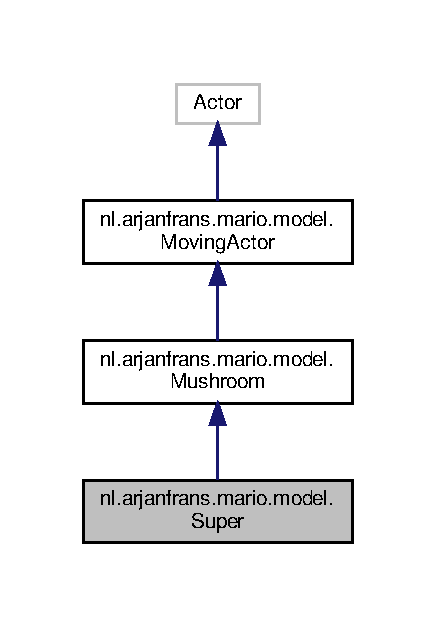
\includegraphics[width=209pt]{classnl_1_1arjanfrans_1_1mario_1_1model_1_1Super__inherit__graph}
\end{center}
\end{figure}


Collaboration diagram for nl.\+arjanfrans.\+mario.\+model.\+Super\+:
\nopagebreak
\begin{figure}[H]
\begin{center}
\leavevmode
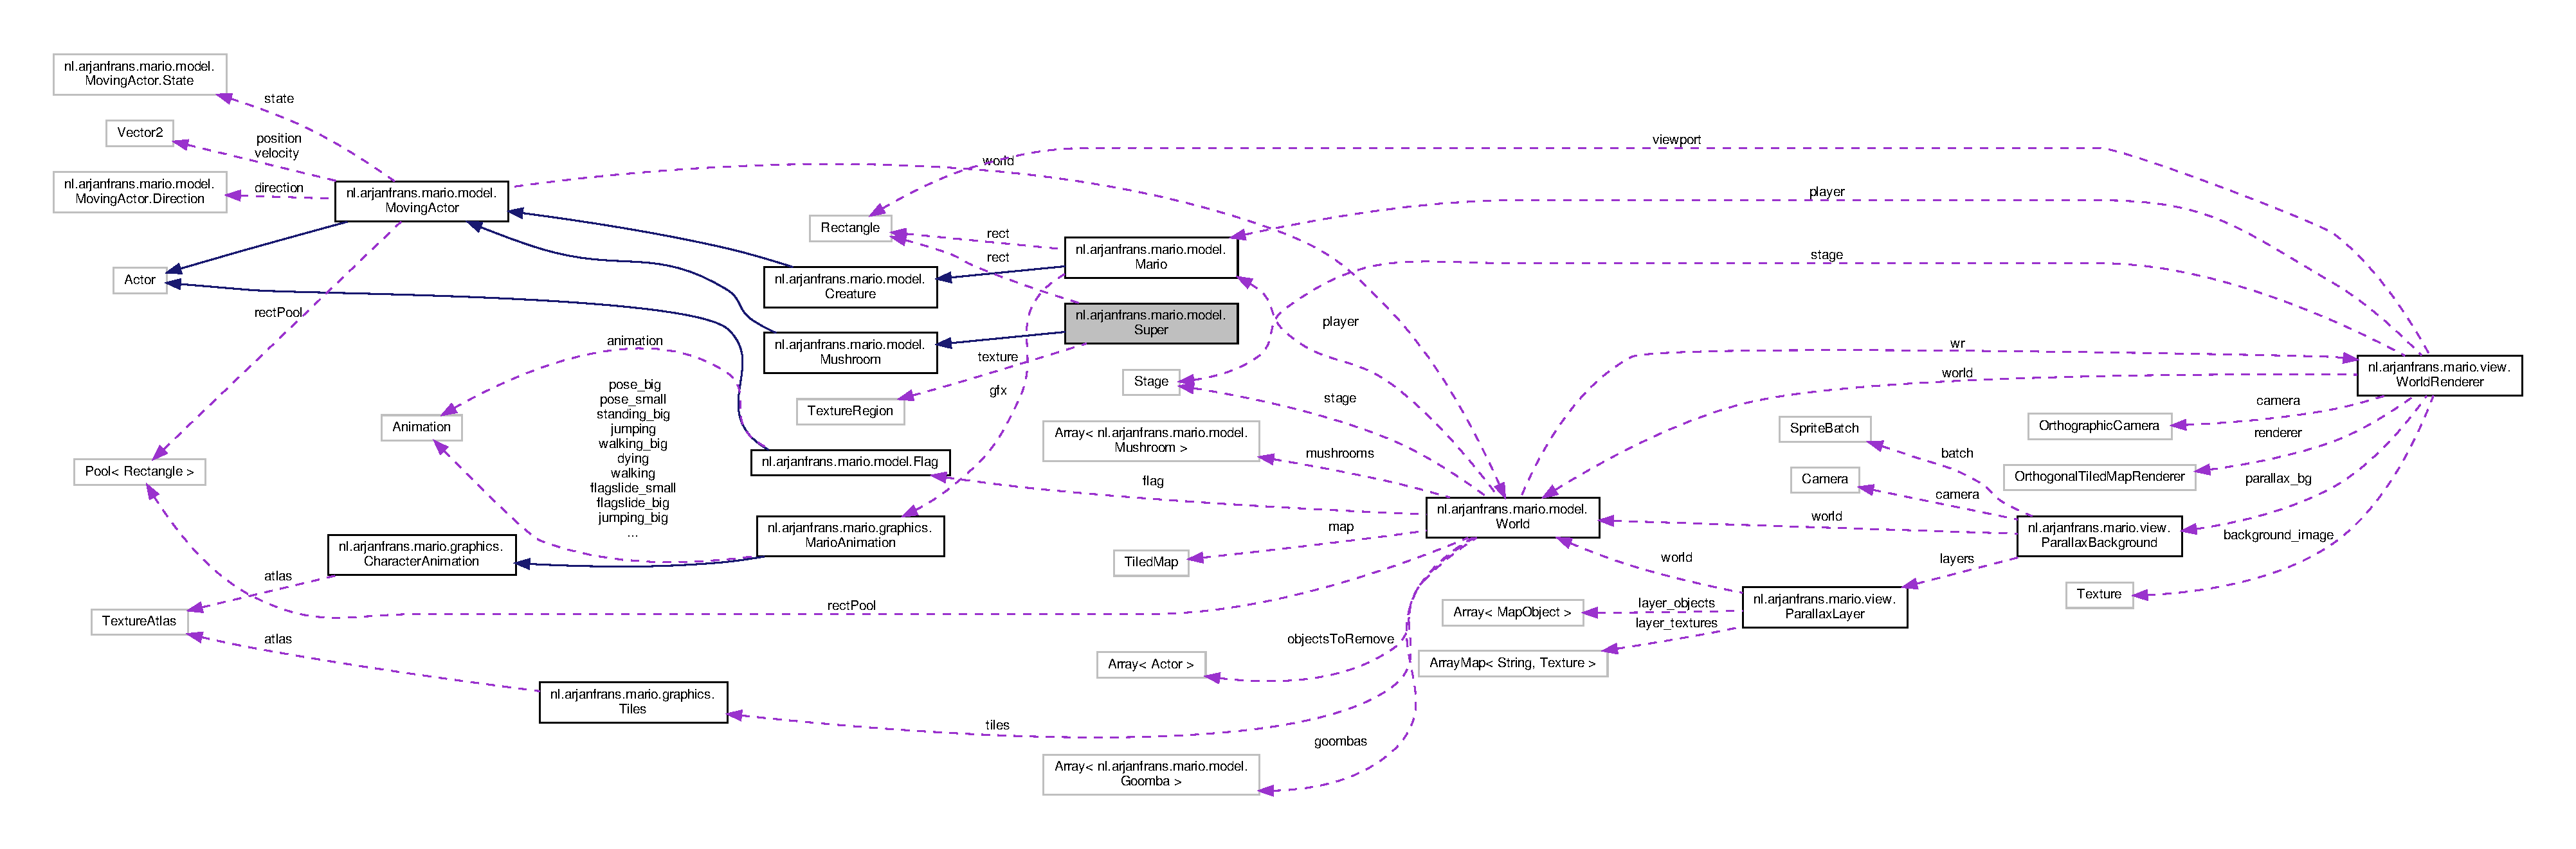
\includegraphics[width=350pt]{classnl_1_1arjanfrans_1_1mario_1_1model_1_1Super__coll__graph}
\end{center}
\end{figure}
\subsection*{Public Member Functions}
\begin{DoxyCompactItemize}
\item 
\hyperlink{classnl_1_1arjanfrans_1_1mario_1_1model_1_1Super_ae31b2b33e224cd5db2e05aabc2e199d8}{Super} (\hyperlink{classnl_1_1arjanfrans_1_1mario_1_1model_1_1World}{World} world, float x, float y, float max\+\_\+velocity)
\begin{DoxyCompactList}\small\item\em Constructor method. \end{DoxyCompactList}\item 
void \hyperlink{classnl_1_1arjanfrans_1_1mario_1_1model_1_1Super_a07b8616c015473a84a5fc9a4108c9995}{draw} (Batch batch, float parent\+Alpha)
\item 
void \hyperlink{classnl_1_1arjanfrans_1_1mario_1_1model_1_1Super_a223190b10a7e63d5057f71cba6e60675}{act} (float delta)
\item 
void \hyperlink{classnl_1_1arjanfrans_1_1mario_1_1model_1_1Super_a10d5cd8618339a32260cdd5bed6ad4dd}{dispose} ()
\begin{DoxyCompactList}\small\item\em Dispose mushroom. \end{DoxyCompactList}\end{DoxyCompactItemize}
\subsection*{Protected Member Functions}
\begin{DoxyCompactItemize}
\item 
void \hyperlink{classnl_1_1arjanfrans_1_1mario_1_1model_1_1Super_a42fb98695c2b31d9078cbe864167ad9d}{die\+By\+Falling} ()
\begin{DoxyCompactList}\small\item\em This method is an abstract method handled by the inherited class. \end{DoxyCompactList}\item 
void \hyperlink{classnl_1_1arjanfrans_1_1mario_1_1model_1_1Super_a71c70031aa0752fb4b2917aa4911f68d}{collision\+X\+Action} ()
\begin{DoxyCompactList}\small\item\em This method is an abstract method handled by the inherited class. \end{DoxyCompactList}\end{DoxyCompactItemize}
\subsection*{Protected Attributes}
\begin{DoxyCompactItemize}
\item 
\mbox{\Hypertarget{classnl_1_1arjanfrans_1_1mario_1_1model_1_1Super_a7be59d0c68b7edcb3d25bd1cd52d48a2}\label{classnl_1_1arjanfrans_1_1mario_1_1model_1_1Super_a7be59d0c68b7edcb3d25bd1cd52d48a2}} 
Rectangle {\bfseries rect} = new Rectangle()
\end{DoxyCompactItemize}
\subsection*{Static Private Attributes}
\begin{DoxyCompactItemize}
\item 
\mbox{\Hypertarget{classnl_1_1arjanfrans_1_1mario_1_1model_1_1Super_ad7b7fb471cfa5965bee27e54904d19f7}\label{classnl_1_1arjanfrans_1_1mario_1_1model_1_1Super_ad7b7fb471cfa5965bee27e54904d19f7}} 
static Texture\+Region {\bfseries texture}
\end{DoxyCompactItemize}


\subsection{Detailed Description}
Inherited class that overrides \hyperlink{classnl_1_1arjanfrans_1_1mario_1_1model_1_1Mushroom}{Mushroom} methods that represents mario in super state. 

\subsection{Constructor \& Destructor Documentation}
\mbox{\Hypertarget{classnl_1_1arjanfrans_1_1mario_1_1model_1_1Super_ae31b2b33e224cd5db2e05aabc2e199d8}\label{classnl_1_1arjanfrans_1_1mario_1_1model_1_1Super_ae31b2b33e224cd5db2e05aabc2e199d8}} 
\index{nl\+::arjanfrans\+::mario\+::model\+::\+Super@{nl\+::arjanfrans\+::mario\+::model\+::\+Super}!Super@{Super}}
\index{Super@{Super}!nl\+::arjanfrans\+::mario\+::model\+::\+Super@{nl\+::arjanfrans\+::mario\+::model\+::\+Super}}
\subsubsection{\texorpdfstring{Super()}{Super()}}
{\footnotesize\ttfamily nl.\+arjanfrans.\+mario.\+model.\+Super.\+Super (\begin{DoxyParamCaption}\item[{\hyperlink{classnl_1_1arjanfrans_1_1mario_1_1model_1_1World}{World}}]{world,  }\item[{float}]{x,  }\item[{float}]{y,  }\item[{float}]{max\+\_\+velocity }\end{DoxyParamCaption})}



Constructor method. 

Method which initializes an instance of \hyperlink{classnl_1_1arjanfrans_1_1mario_1_1model_1_1Super}{Super} 
\begin{DoxyParams}{Parameters}
{\em world} & The world object in which \hyperlink{classnl_1_1arjanfrans_1_1mario_1_1model_1_1Mario}{Mario} will exist in \\
\hline
{\em x} & coordinate of super mushroom \\
\hline
{\em y} & coordinate of super mushroom \\
\hline
{\em max\+\_\+velocity} & of super mushroom \\
\hline
\end{DoxyParams}


\subsection{Member Function Documentation}
\mbox{\Hypertarget{classnl_1_1arjanfrans_1_1mario_1_1model_1_1Super_a223190b10a7e63d5057f71cba6e60675}\label{classnl_1_1arjanfrans_1_1mario_1_1model_1_1Super_a223190b10a7e63d5057f71cba6e60675}} 
\index{nl\+::arjanfrans\+::mario\+::model\+::\+Super@{nl\+::arjanfrans\+::mario\+::model\+::\+Super}!act@{act}}
\index{act@{act}!nl\+::arjanfrans\+::mario\+::model\+::\+Super@{nl\+::arjanfrans\+::mario\+::model\+::\+Super}}
\subsubsection{\texorpdfstring{act()}{act()}}
{\footnotesize\ttfamily void nl.\+arjanfrans.\+mario.\+model.\+Super.\+act (\begin{DoxyParamCaption}\item[{float}]{delta }\end{DoxyParamCaption})}





\mbox{\Hypertarget{classnl_1_1arjanfrans_1_1mario_1_1model_1_1Super_a71c70031aa0752fb4b2917aa4911f68d}\label{classnl_1_1arjanfrans_1_1mario_1_1model_1_1Super_a71c70031aa0752fb4b2917aa4911f68d}} 
\index{nl\+::arjanfrans\+::mario\+::model\+::\+Super@{nl\+::arjanfrans\+::mario\+::model\+::\+Super}!collision\+X\+Action@{collision\+X\+Action}}
\index{collision\+X\+Action@{collision\+X\+Action}!nl\+::arjanfrans\+::mario\+::model\+::\+Super@{nl\+::arjanfrans\+::mario\+::model\+::\+Super}}
\subsubsection{\texorpdfstring{collision\+X\+Action()}{collisionXAction()}}
{\footnotesize\ttfamily void nl.\+arjanfrans.\+mario.\+model.\+Super.\+collision\+X\+Action (\begin{DoxyParamCaption}{ }\end{DoxyParamCaption})\hspace{0.3cm}{\ttfamily [protected]}}



This method is an abstract method handled by the inherited class. 

\mbox{\Hypertarget{classnl_1_1arjanfrans_1_1mario_1_1model_1_1Super_a42fb98695c2b31d9078cbe864167ad9d}\label{classnl_1_1arjanfrans_1_1mario_1_1model_1_1Super_a42fb98695c2b31d9078cbe864167ad9d}} 
\index{nl\+::arjanfrans\+::mario\+::model\+::\+Super@{nl\+::arjanfrans\+::mario\+::model\+::\+Super}!die\+By\+Falling@{die\+By\+Falling}}
\index{die\+By\+Falling@{die\+By\+Falling}!nl\+::arjanfrans\+::mario\+::model\+::\+Super@{nl\+::arjanfrans\+::mario\+::model\+::\+Super}}
\subsubsection{\texorpdfstring{die\+By\+Falling()}{dieByFalling()}}
{\footnotesize\ttfamily void nl.\+arjanfrans.\+mario.\+model.\+Super.\+die\+By\+Falling (\begin{DoxyParamCaption}{ }\end{DoxyParamCaption})\hspace{0.3cm}{\ttfamily [protected]}}



This method is an abstract method handled by the inherited class. 

\mbox{\Hypertarget{classnl_1_1arjanfrans_1_1mario_1_1model_1_1Super_a10d5cd8618339a32260cdd5bed6ad4dd}\label{classnl_1_1arjanfrans_1_1mario_1_1model_1_1Super_a10d5cd8618339a32260cdd5bed6ad4dd}} 
\index{nl\+::arjanfrans\+::mario\+::model\+::\+Super@{nl\+::arjanfrans\+::mario\+::model\+::\+Super}!dispose@{dispose}}
\index{dispose@{dispose}!nl\+::arjanfrans\+::mario\+::model\+::\+Super@{nl\+::arjanfrans\+::mario\+::model\+::\+Super}}
\subsubsection{\texorpdfstring{dispose()}{dispose()}}
{\footnotesize\ttfamily void nl.\+arjanfrans.\+mario.\+model.\+Super.\+dispose (\begin{DoxyParamCaption}{ }\end{DoxyParamCaption})}



Dispose mushroom. 

\mbox{\Hypertarget{classnl_1_1arjanfrans_1_1mario_1_1model_1_1Super_a07b8616c015473a84a5fc9a4108c9995}\label{classnl_1_1arjanfrans_1_1mario_1_1model_1_1Super_a07b8616c015473a84a5fc9a4108c9995}} 
\index{nl\+::arjanfrans\+::mario\+::model\+::\+Super@{nl\+::arjanfrans\+::mario\+::model\+::\+Super}!draw@{draw}}
\index{draw@{draw}!nl\+::arjanfrans\+::mario\+::model\+::\+Super@{nl\+::arjanfrans\+::mario\+::model\+::\+Super}}
\subsubsection{\texorpdfstring{draw()}{draw()}}
{\footnotesize\ttfamily void nl.\+arjanfrans.\+mario.\+model.\+Super.\+draw (\begin{DoxyParamCaption}\item[{Batch}]{batch,  }\item[{float}]{parent\+Alpha }\end{DoxyParamCaption})}







The documentation for this class was generated from the following file\+:\begin{DoxyCompactItemize}
\item 
core/src/nl/arjanfrans/mario/model/\hyperlink{Super_8java}{Super.\+java}\end{DoxyCompactItemize}

\hypertarget{classnl_1_1arjanfrans_1_1mario_1_1model_1_1Tile}{}\section{nl.\+arjanfrans.\+mario.\+model.\+Tile Class Reference}
\label{classnl_1_1arjanfrans_1_1mario_1_1model_1_1Tile}\index{nl.\+arjanfrans.\+mario.\+model.\+Tile@{nl.\+arjanfrans.\+mario.\+model.\+Tile}}


Inheritance diagram for nl.\+arjanfrans.\+mario.\+model.\+Tile\+:\nopagebreak
\begin{figure}[H]
\begin{center}
\leavevmode
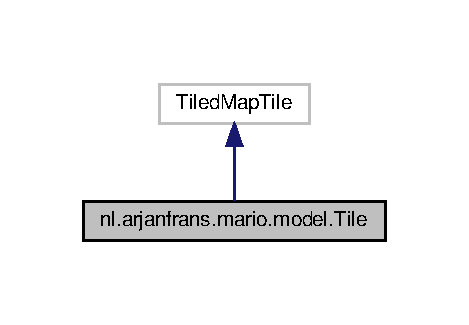
\includegraphics[width=225pt]{classnl_1_1arjanfrans_1_1mario_1_1model_1_1Tile__inherit__graph}
\end{center}
\end{figure}


Collaboration diagram for nl.\+arjanfrans.\+mario.\+model.\+Tile\+:\nopagebreak
\begin{figure}[H]
\begin{center}
\leavevmode
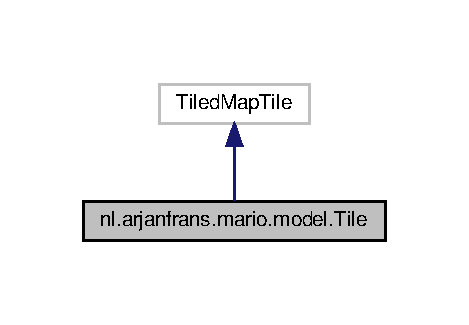
\includegraphics[width=225pt]{classnl_1_1arjanfrans_1_1mario_1_1model_1_1Tile__coll__graph}
\end{center}
\end{figure}
\subsection*{Public Member Functions}
\begin{DoxyCompactItemize}
\item 
\mbox{\Hypertarget{classnl_1_1arjanfrans_1_1mario_1_1model_1_1Tile_a936ccffb6b17ccfd84450edff0aadf03}\label{classnl_1_1arjanfrans_1_1mario_1_1model_1_1Tile_a936ccffb6b17ccfd84450edff0aadf03}} 
int {\bfseries get\+Id} ()
\item 
\mbox{\Hypertarget{classnl_1_1arjanfrans_1_1mario_1_1model_1_1Tile_a86fd5aa7a4544e10dd7597f238245f77}\label{classnl_1_1arjanfrans_1_1mario_1_1model_1_1Tile_a86fd5aa7a4544e10dd7597f238245f77}} 
void {\bfseries set\+Id} (int id)
\item 
\mbox{\Hypertarget{classnl_1_1arjanfrans_1_1mario_1_1model_1_1Tile_ac2e9cbb680eeb3caadb1c614a66049f7}\label{classnl_1_1arjanfrans_1_1mario_1_1model_1_1Tile_ac2e9cbb680eeb3caadb1c614a66049f7}} 
Blend\+Mode {\bfseries get\+Blend\+Mode} ()
\item 
\mbox{\Hypertarget{classnl_1_1arjanfrans_1_1mario_1_1model_1_1Tile_a5e15b8a0fb73af3da56a07be0f0176e8}\label{classnl_1_1arjanfrans_1_1mario_1_1model_1_1Tile_a5e15b8a0fb73af3da56a07be0f0176e8}} 
void {\bfseries set\+Blend\+Mode} (Blend\+Mode blend\+Mode)
\item 
\mbox{\Hypertarget{classnl_1_1arjanfrans_1_1mario_1_1model_1_1Tile_a8ed2f182e9907c254597fff487cae146}\label{classnl_1_1arjanfrans_1_1mario_1_1model_1_1Tile_a8ed2f182e9907c254597fff487cae146}} 
Texture\+Region {\bfseries get\+Texture\+Region} ()
\item 
\mbox{\Hypertarget{classnl_1_1arjanfrans_1_1mario_1_1model_1_1Tile_adb386d505d43773473324757c158659f}\label{classnl_1_1arjanfrans_1_1mario_1_1model_1_1Tile_adb386d505d43773473324757c158659f}} 
void {\bfseries set\+Texture\+Region} (Texture\+Region texture\+Region)
\item 
\mbox{\Hypertarget{classnl_1_1arjanfrans_1_1mario_1_1model_1_1Tile_a55dc285ea0024afe988f0e215a1cc0ec}\label{classnl_1_1arjanfrans_1_1mario_1_1model_1_1Tile_a55dc285ea0024afe988f0e215a1cc0ec}} 
Map\+Properties {\bfseries get\+Properties} ()
\item 
\mbox{\Hypertarget{classnl_1_1arjanfrans_1_1mario_1_1model_1_1Tile_a6fc4fc889d5f58d2aa8e783082fdc50e}\label{classnl_1_1arjanfrans_1_1mario_1_1model_1_1Tile_a6fc4fc889d5f58d2aa8e783082fdc50e}} 
float {\bfseries get\+OffsetX} ()
\item 
\mbox{\Hypertarget{classnl_1_1arjanfrans_1_1mario_1_1model_1_1Tile_a3c79a1c221004c147c3040776e4cdd10}\label{classnl_1_1arjanfrans_1_1mario_1_1model_1_1Tile_a3c79a1c221004c147c3040776e4cdd10}} 
void {\bfseries set\+OffsetX} (float offsetX)
\item 
\mbox{\Hypertarget{classnl_1_1arjanfrans_1_1mario_1_1model_1_1Tile_ac86196e0de9a6e33910ac046a4dbe03c}\label{classnl_1_1arjanfrans_1_1mario_1_1model_1_1Tile_ac86196e0de9a6e33910ac046a4dbe03c}} 
float {\bfseries get\+OffsetY} ()
\item 
\mbox{\Hypertarget{classnl_1_1arjanfrans_1_1mario_1_1model_1_1Tile_a841263b4394886e8581d783292eb1132}\label{classnl_1_1arjanfrans_1_1mario_1_1model_1_1Tile_a841263b4394886e8581d783292eb1132}} 
void {\bfseries set\+OffsetY} (float offsetY)
\end{DoxyCompactItemize}


The documentation for this class was generated from the following file\+:\begin{DoxyCompactItemize}
\item 
core/src/nl/arjanfrans/mario/model/Tile.\+java\end{DoxyCompactItemize}

\hypertarget{classnl_1_1arjanfrans_1_1mario_1_1graphics_1_1Tiles}{}\section{nl.\+arjanfrans.\+mario.\+graphics.\+Tiles Class Reference}
\label{classnl_1_1arjanfrans_1_1mario_1_1graphics_1_1Tiles}\index{nl.\+arjanfrans.\+mario.\+graphics.\+Tiles@{nl.\+arjanfrans.\+mario.\+graphics.\+Tiles}}


This is a class meant to deal with the tiles that make up the graphics of the game.  




Collaboration diagram for nl.\+arjanfrans.\+mario.\+graphics.\+Tiles\+:\nopagebreak
\begin{figure}[H]
\begin{center}
\leavevmode
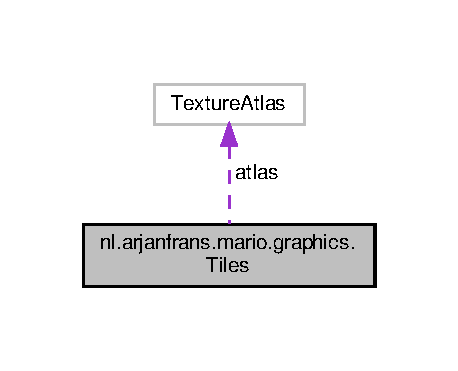
\includegraphics[width=220pt]{classnl_1_1arjanfrans_1_1mario_1_1graphics_1_1Tiles__coll__graph}
\end{center}
\end{figure}
\subsection*{Public Member Functions}
\begin{DoxyCompactItemize}
\item 
\mbox{\Hypertarget{classnl_1_1arjanfrans_1_1mario_1_1graphics_1_1Tiles_a6e93b266076f60eeda8661bc0619dd8a}\label{classnl_1_1arjanfrans_1_1mario_1_1graphics_1_1Tiles_a6e93b266076f60eeda8661bc0619dd8a}} 
void \hyperlink{classnl_1_1arjanfrans_1_1mario_1_1graphics_1_1Tiles_a6e93b266076f60eeda8661bc0619dd8a}{dispose} ()
\begin{DoxyCompactList}\small\item\em A method meant to dipose of the atlas file. \end{DoxyCompactList}\end{DoxyCompactItemize}
\subsection*{Static Public Member Functions}
\begin{DoxyCompactItemize}
\item 
static Array$<$ Static\+Tiled\+Map\+Tile $>$ \hyperlink{classnl_1_1arjanfrans_1_1mario_1_1graphics_1_1Tiles_a032fa48452ac57c65e8e86c23a28f0ee}{get\+Animated\+Tile} (String name)
\begin{DoxyCompactList}\small\item\em A method meant to retrieve an animation tile based on the name of the animation. \end{DoxyCompactList}\item 
static Animation \hyperlink{classnl_1_1arjanfrans_1_1mario_1_1graphics_1_1Tiles_a2448c85397533ac26d5c0159e7746e1a}{get\+Animation} (float speed, String name)
\begin{DoxyCompactList}\small\item\em A method meant to retrieve an animation based on the name of the animation. \end{DoxyCompactList}\item 
static Texture\+Region \hyperlink{classnl_1_1arjanfrans_1_1mario_1_1graphics_1_1Tiles_a33e1805fc683bac7f3883119857486eb}{get\+Tile} (String name)
\begin{DoxyCompactList}\small\item\em A method meant to find a tile in a tile sheet based on the named indicated for it in the atlas file. \end{DoxyCompactList}\item 
static Texture\+Region \hyperlink{classnl_1_1arjanfrans_1_1mario_1_1graphics_1_1Tiles_aec062c35528937ca08a65a3e5b120d91}{get\+Tile8} (String name)
\begin{DoxyCompactList}\small\item\em A method meant to find a tile (split into to sets of eight pixels) in a tile sheet based on the named indicated for it in the atlas file. \end{DoxyCompactList}\end{DoxyCompactItemize}
\subsection*{Static Private Attributes}
\begin{DoxyCompactItemize}
\item 
\mbox{\Hypertarget{classnl_1_1arjanfrans_1_1mario_1_1graphics_1_1Tiles_a7de5b9b53e9a767b5ddf60b6b6e282e4}\label{classnl_1_1arjanfrans_1_1mario_1_1graphics_1_1Tiles_a7de5b9b53e9a767b5ddf60b6b6e282e4}} 
static Texture\+Atlas {\bfseries atlas} = new Texture\+Atlas(\char`\"{}data/tiles/mario\+\_\+tileset.\+atlas\char`\"{})
\end{DoxyCompactItemize}


\subsection{Detailed Description}
This is a class meant to deal with the tiles that make up the graphics of the game. 

\subsection{Member Function Documentation}
\mbox{\Hypertarget{classnl_1_1arjanfrans_1_1mario_1_1graphics_1_1Tiles_a032fa48452ac57c65e8e86c23a28f0ee}\label{classnl_1_1arjanfrans_1_1mario_1_1graphics_1_1Tiles_a032fa48452ac57c65e8e86c23a28f0ee}} 
\index{nl\+::arjanfrans\+::mario\+::graphics\+::\+Tiles@{nl\+::arjanfrans\+::mario\+::graphics\+::\+Tiles}!get\+Animated\+Tile@{get\+Animated\+Tile}}
\index{get\+Animated\+Tile@{get\+Animated\+Tile}!nl\+::arjanfrans\+::mario\+::graphics\+::\+Tiles@{nl\+::arjanfrans\+::mario\+::graphics\+::\+Tiles}}
\subsubsection{\texorpdfstring{get\+Animated\+Tile()}{getAnimatedTile()}}
{\footnotesize\ttfamily static Array$<$Static\+Tiled\+Map\+Tile$>$ nl.\+arjanfrans.\+mario.\+graphics.\+Tiles.\+get\+Animated\+Tile (\begin{DoxyParamCaption}\item[{String}]{name }\end{DoxyParamCaption})\hspace{0.3cm}{\ttfamily [static]}}



A method meant to retrieve an animation tile based on the name of the animation. 


\begin{DoxyParams}{Parameters}
{\em name} & -\/ the name of the animation found in the mario\+\_\+tileset.\+atlas file. \\
\hline
\end{DoxyParams}
\begin{DoxyReturn}{Returns}
an array of Static\+Tiled\+Map\+Tile, representing the frames of the Animation. 
\end{DoxyReturn}
\mbox{\Hypertarget{classnl_1_1arjanfrans_1_1mario_1_1graphics_1_1Tiles_a2448c85397533ac26d5c0159e7746e1a}\label{classnl_1_1arjanfrans_1_1mario_1_1graphics_1_1Tiles_a2448c85397533ac26d5c0159e7746e1a}} 
\index{nl\+::arjanfrans\+::mario\+::graphics\+::\+Tiles@{nl\+::arjanfrans\+::mario\+::graphics\+::\+Tiles}!get\+Animation@{get\+Animation}}
\index{get\+Animation@{get\+Animation}!nl\+::arjanfrans\+::mario\+::graphics\+::\+Tiles@{nl\+::arjanfrans\+::mario\+::graphics\+::\+Tiles}}
\subsubsection{\texorpdfstring{get\+Animation()}{getAnimation()}}
{\footnotesize\ttfamily static Animation nl.\+arjanfrans.\+mario.\+graphics.\+Tiles.\+get\+Animation (\begin{DoxyParamCaption}\item[{float}]{speed,  }\item[{String}]{name }\end{DoxyParamCaption})\hspace{0.3cm}{\ttfamily [static]}}



A method meant to retrieve an animation based on the name of the animation. 


\begin{DoxyParams}{Parameters}
{\em name} & -\/ the name of the animation found in the mario\+\_\+tileset.\+atlas file. \\
\hline
{\em speed} & -\/ a float representing how fast the frames are to be moved through. \\
\hline
\end{DoxyParams}
\begin{DoxyReturn}{Returns}
an Animation object, representing the Animation named. 
\end{DoxyReturn}
\mbox{\Hypertarget{classnl_1_1arjanfrans_1_1mario_1_1graphics_1_1Tiles_a33e1805fc683bac7f3883119857486eb}\label{classnl_1_1arjanfrans_1_1mario_1_1graphics_1_1Tiles_a33e1805fc683bac7f3883119857486eb}} 
\index{nl\+::arjanfrans\+::mario\+::graphics\+::\+Tiles@{nl\+::arjanfrans\+::mario\+::graphics\+::\+Tiles}!get\+Tile@{get\+Tile}}
\index{get\+Tile@{get\+Tile}!nl\+::arjanfrans\+::mario\+::graphics\+::\+Tiles@{nl\+::arjanfrans\+::mario\+::graphics\+::\+Tiles}}
\subsubsection{\texorpdfstring{get\+Tile()}{getTile()}}
{\footnotesize\ttfamily static Texture\+Region nl.\+arjanfrans.\+mario.\+graphics.\+Tiles.\+get\+Tile (\begin{DoxyParamCaption}\item[{String}]{name }\end{DoxyParamCaption})\hspace{0.3cm}{\ttfamily [static]}}



A method meant to find a tile in a tile sheet based on the named indicated for it in the atlas file. 


\begin{DoxyParams}{Parameters}
{\em name} & -\/ the name of the tile found in the mario\+\_\+tileset.\+atlas file. \\
\hline
\end{DoxyParams}
\begin{DoxyReturn}{Returns}
a Texture\+Region object which represents the tile\textquotesingle{}s location on a tile sheet 
\end{DoxyReturn}
\mbox{\Hypertarget{classnl_1_1arjanfrans_1_1mario_1_1graphics_1_1Tiles_aec062c35528937ca08a65a3e5b120d91}\label{classnl_1_1arjanfrans_1_1mario_1_1graphics_1_1Tiles_aec062c35528937ca08a65a3e5b120d91}} 
\index{nl\+::arjanfrans\+::mario\+::graphics\+::\+Tiles@{nl\+::arjanfrans\+::mario\+::graphics\+::\+Tiles}!get\+Tile8@{get\+Tile8}}
\index{get\+Tile8@{get\+Tile8}!nl\+::arjanfrans\+::mario\+::graphics\+::\+Tiles@{nl\+::arjanfrans\+::mario\+::graphics\+::\+Tiles}}
\subsubsection{\texorpdfstring{get\+Tile8()}{getTile8()}}
{\footnotesize\ttfamily static Texture\+Region nl.\+arjanfrans.\+mario.\+graphics.\+Tiles.\+get\+Tile8 (\begin{DoxyParamCaption}\item[{String}]{name }\end{DoxyParamCaption})\hspace{0.3cm}{\ttfamily [static]}}



A method meant to find a tile (split into to sets of eight pixels) in a tile sheet based on the named indicated for it in the atlas file. 


\begin{DoxyParams}{Parameters}
{\em name} & -\/ the name of the tile found in the mario\+\_\+tileset.\+atlas file. \\
\hline
\end{DoxyParams}
\begin{DoxyReturn}{Returns}
a Texture\+Region object which represents the tile\textquotesingle{}s location on a tile sheet 
\end{DoxyReturn}


The documentation for this class was generated from the following file\+:\begin{DoxyCompactItemize}
\item 
core/src/nl/arjanfrans/mario/graphics/Tiles.\+java\end{DoxyCompactItemize}

\hypertarget{classnl_1_1arjanfrans_1_1mario_1_1model_1_1World}{}\section{nl.\+arjanfrans.\+mario.\+model.\+World Class Reference}
\label{classnl_1_1arjanfrans_1_1mario_1_1model_1_1World}\index{nl.\+arjanfrans.\+mario.\+model.\+World@{nl.\+arjanfrans.\+mario.\+model.\+World}}


Represents world.  




Collaboration diagram for nl.\+arjanfrans.\+mario.\+model.\+World\+:
\nopagebreak
\begin{figure}[H]
\begin{center}
\leavevmode
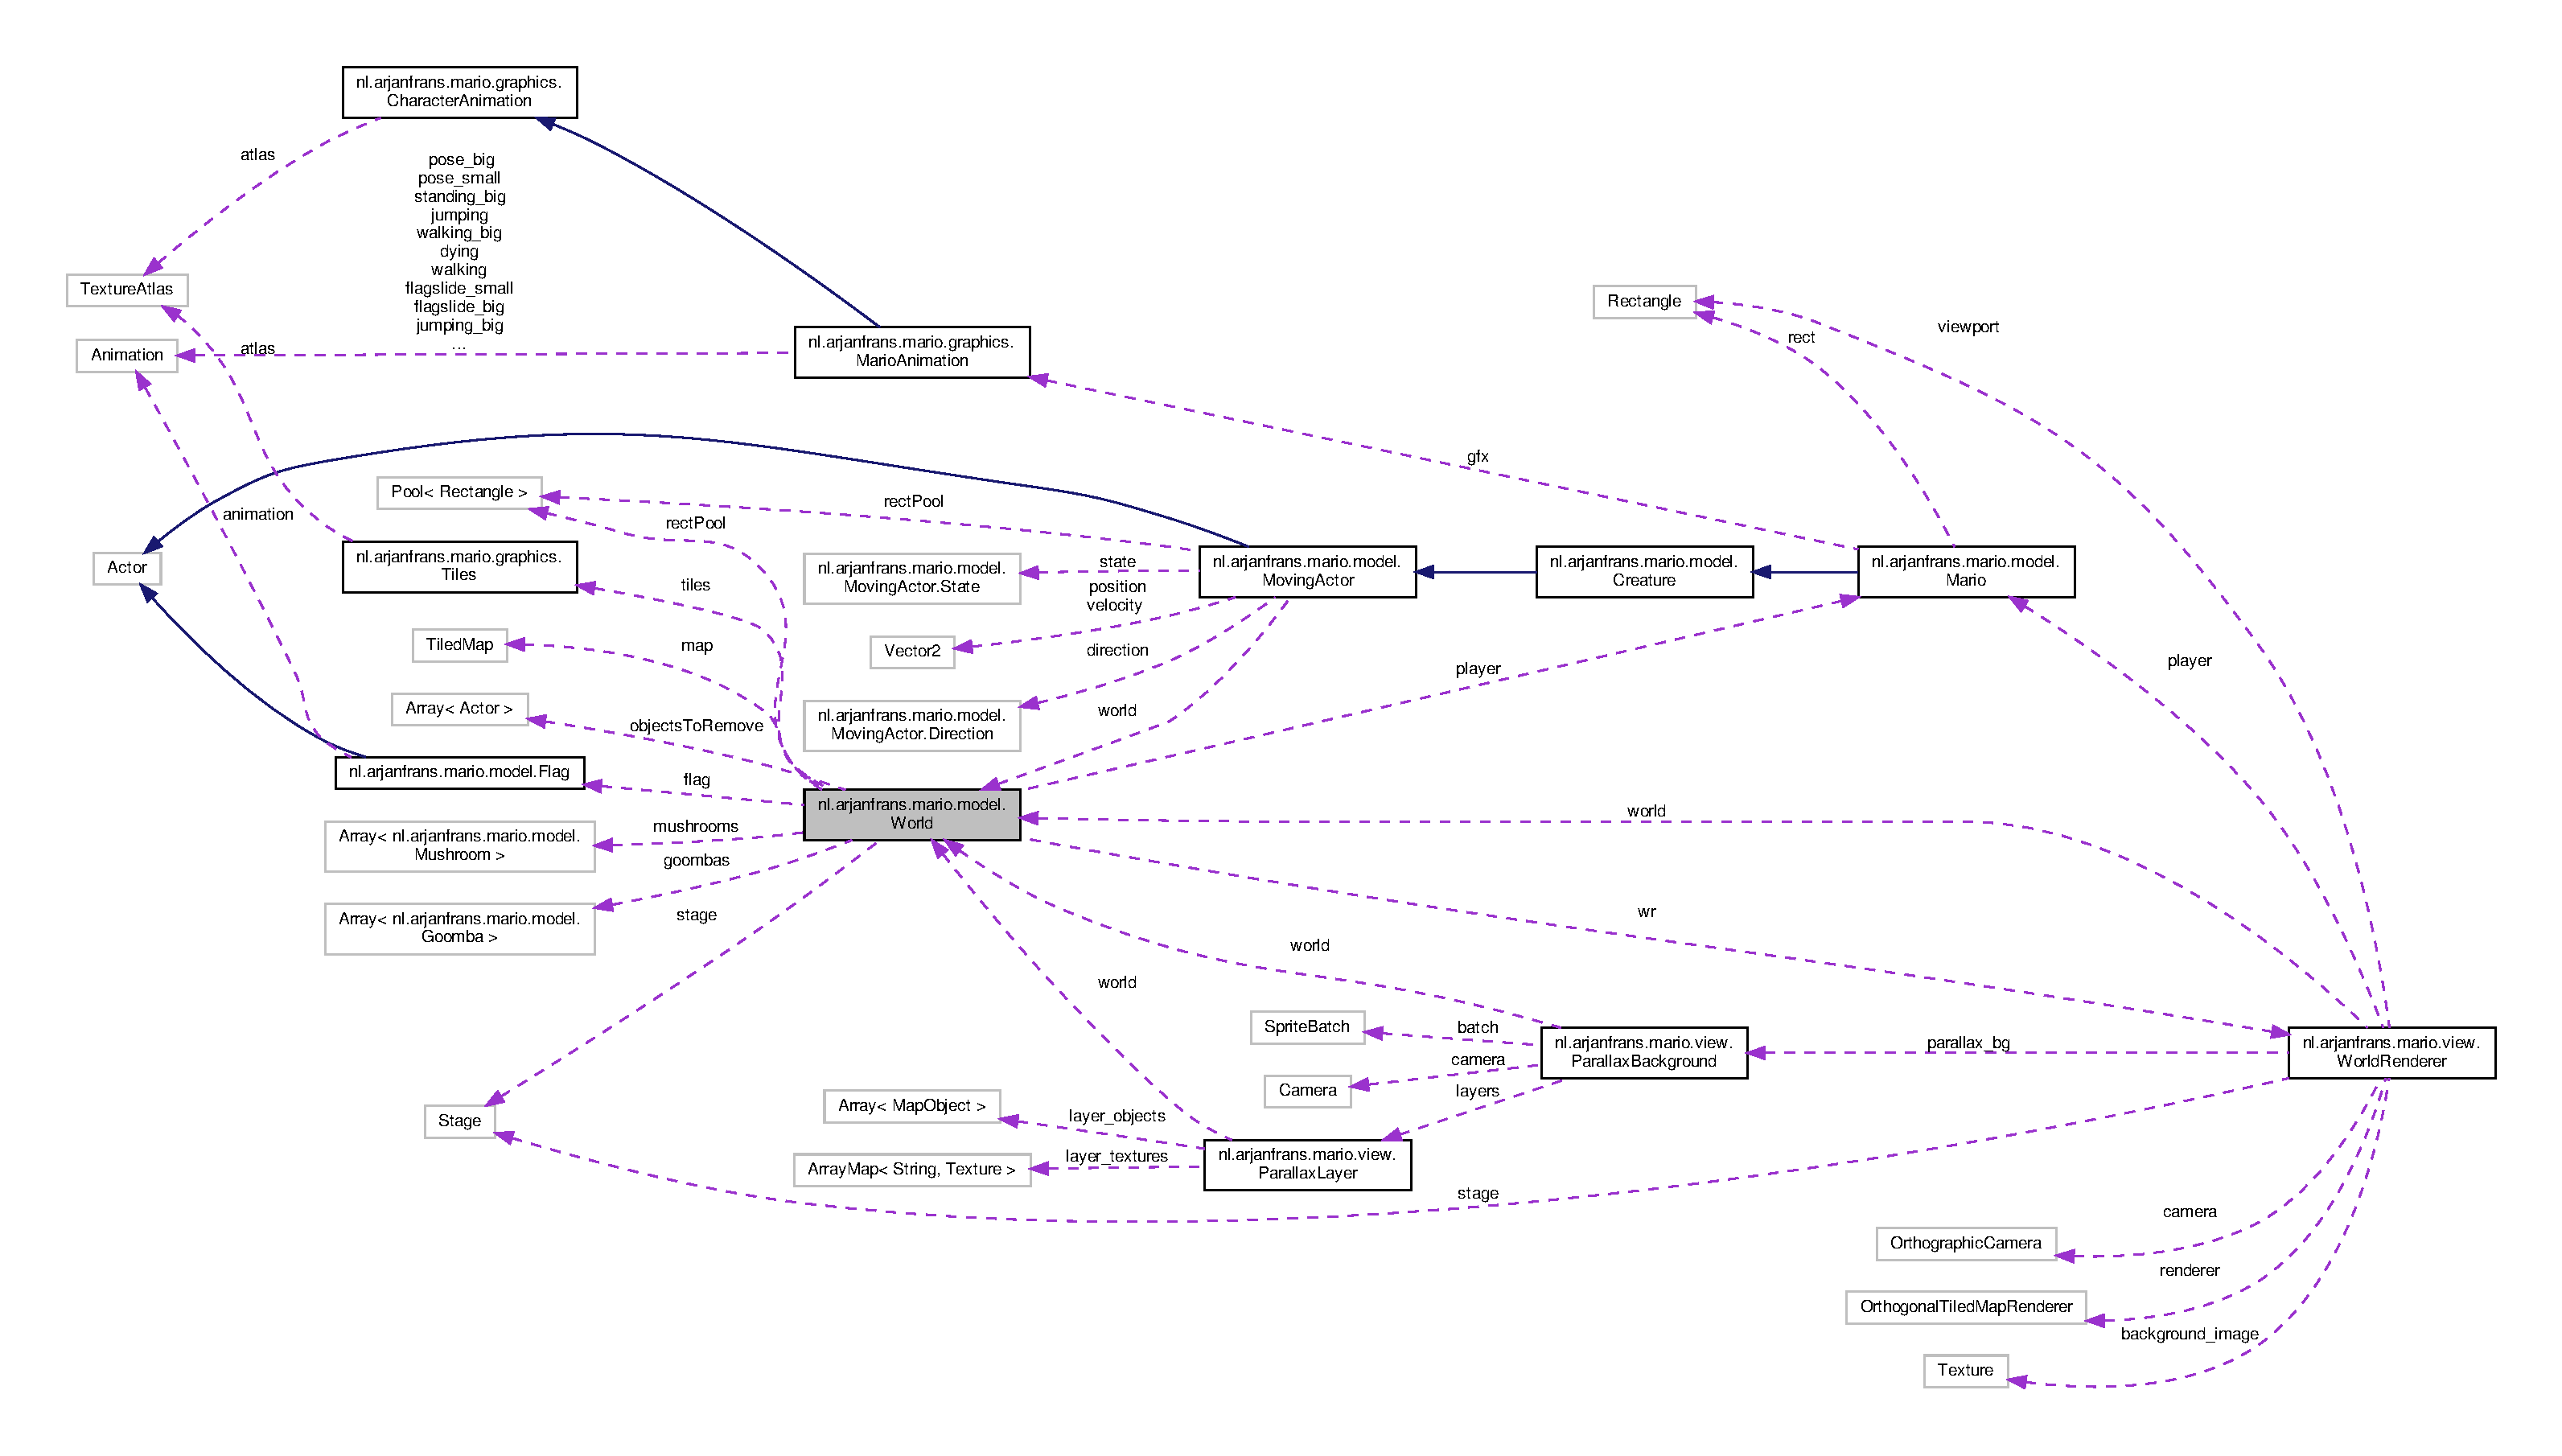
\includegraphics[width=350pt]{classnl_1_1arjanfrans_1_1mario_1_1model_1_1World__coll__graph}
\end{center}
\end{figure}
\subsection*{Public Member Functions}
\begin{DoxyCompactItemize}
\item 
\hyperlink{classnl_1_1arjanfrans_1_1mario_1_1model_1_1World_abc0eb7717682f6f00f139647207d425b}{World} ()
\begin{DoxyCompactList}\small\item\em Constructor method. \end{DoxyCompactList}\item 
void \hyperlink{classnl_1_1arjanfrans_1_1mario_1_1model_1_1World_a73b951d2722bc1984021d0e4da644008}{remove\+Actor} (Actor a)
\begin{DoxyCompactList}\small\item\em Removes actor. \end{DoxyCompactList}\item 
\mbox{\Hypertarget{classnl_1_1arjanfrans_1_1mario_1_1model_1_1World_a09caf085ce851f56c9773c9c83e3eff8}\label{classnl_1_1arjanfrans_1_1mario_1_1model_1_1World_a09caf085ce851f56c9773c9c83e3eff8}} 
void \hyperlink{classnl_1_1arjanfrans_1_1mario_1_1model_1_1World_a09caf085ce851f56c9773c9c83e3eff8}{update} ()
\begin{DoxyCompactList}\small\item\em Updates world. \end{DoxyCompactList}\item 
Array$<$ \hyperlink{classnl_1_1arjanfrans_1_1mario_1_1model_1_1StaticActor}{Static\+Actor} $>$ \hyperlink{classnl_1_1arjanfrans_1_1mario_1_1model_1_1World_a1f0db37c4fbacb1048e6cd13725305aa}{get\+Static\+Actors} ()
\item 
\hyperlink{classnl_1_1arjanfrans_1_1mario_1_1view_1_1WorldRenderer}{World\+Renderer} \hyperlink{classnl_1_1arjanfrans_1_1mario_1_1model_1_1World_a931f9fe3450c07ec17c8f14dcd3ec58e}{get\+Renderer} ()
\begin{DoxyCompactList}\small\item\em Get render of world. \end{DoxyCompactList}\item 
\hyperlink{classnl_1_1arjanfrans_1_1mario_1_1model_1_1Mario}{Mario} \hyperlink{classnl_1_1arjanfrans_1_1mario_1_1model_1_1World_a08a107e2e429df5092b7bd2198d4553a}{get\+Player} ()
\begin{DoxyCompactList}\small\item\em Get player. \end{DoxyCompactList}\item 
Tiled\+Map \hyperlink{classnl_1_1arjanfrans_1_1mario_1_1model_1_1World_a8812c471d0f3e39ab3a0073527baf4d8}{get\+Map} ()
\begin{DoxyCompactList}\small\item\em Get map of world. \end{DoxyCompactList}\item 
Array$<$ \hyperlink{classnl_1_1arjanfrans_1_1mario_1_1model_1_1Goomba}{Goomba} $>$ \hyperlink{classnl_1_1arjanfrans_1_1mario_1_1model_1_1World_a8d4f869faea3c599334975f5511aca9a}{get\+Enemies} ()
\begin{DoxyCompactList}\small\item\em Get enemies in world. \end{DoxyCompactList}\item 
Array$<$ \hyperlink{classnl_1_1arjanfrans_1_1mario_1_1model_1_1Mushroom}{Mushroom} $>$ \hyperlink{classnl_1_1arjanfrans_1_1mario_1_1model_1_1World_a3acf1e0b7bab1db92c5537fbd038f5c5}{get\+Mushrooms} ()
\begin{DoxyCompactList}\small\item\em Get mushrooms in world. \end{DoxyCompactList}\item 
Array$<$ Rectangle $>$ \hyperlink{classnl_1_1arjanfrans_1_1mario_1_1model_1_1World_ae986617591bfcee4c12343588b9a22b7}{get\+Tiles} (int startX, int startY, int endX, int endY)
\begin{DoxyCompactList}\small\item\em Get tiles of world. \end{DoxyCompactList}\item 
\mbox{\Hypertarget{classnl_1_1arjanfrans_1_1mario_1_1model_1_1World_aa4f564130328b9c3b3cd5ecb0f33985b}\label{classnl_1_1arjanfrans_1_1mario_1_1model_1_1World_aa4f564130328b9c3b3cd5ecb0f33985b}} 
void \hyperlink{classnl_1_1arjanfrans_1_1mario_1_1model_1_1World_aa4f564130328b9c3b3cd5ecb0f33985b}{dispose} ()
\begin{DoxyCompactList}\small\item\em Dispose world. \end{DoxyCompactList}\item 
Stage \hyperlink{classnl_1_1arjanfrans_1_1mario_1_1model_1_1World_ac56b0f98a3e839bbb10bf6efec0e487a}{get\+Stage} ()
\begin{DoxyCompactList}\small\item\em Get stage of world. \end{DoxyCompactList}\end{DoxyCompactItemize}
\subsection*{Static Public Attributes}
\begin{DoxyCompactItemize}
\item 
\mbox{\Hypertarget{classnl_1_1arjanfrans_1_1mario_1_1model_1_1World_a48cc806be51479e40d1a4715e1eef234}\label{classnl_1_1arjanfrans_1_1mario_1_1model_1_1World_a48cc806be51479e40d1a4715e1eef234}} 
static final float {\bfseries G\+R\+A\+V\+I\+TY} = -\/150
\item 
\mbox{\Hypertarget{classnl_1_1arjanfrans_1_1mario_1_1model_1_1World_a46cf4f8f487ef4de0c8e812d81d94a07}\label{classnl_1_1arjanfrans_1_1mario_1_1model_1_1World_a46cf4f8f487ef4de0c8e812d81d94a07}} 
static final float {\bfseries scale} = 1/16f
\item 
\mbox{\Hypertarget{classnl_1_1arjanfrans_1_1mario_1_1model_1_1World_a03d5af92c1c20e4b1d99c2a93b0654f0}\label{classnl_1_1arjanfrans_1_1mario_1_1model_1_1World_a03d5af92c1c20e4b1d99c2a93b0654f0}} 
static boolean {\bfseries reset\+\_\+flag} = false
\item 
\mbox{\Hypertarget{classnl_1_1arjanfrans_1_1mario_1_1model_1_1World_a583d7ea2ce8e985489255cab5e40a035}\label{classnl_1_1arjanfrans_1_1mario_1_1model_1_1World_a583d7ea2ce8e985489255cab5e40a035}} 
static Array$<$ Actor $>$ {\bfseries objects\+To\+Remove} = new Array$<$Actor$>$()
\end{DoxyCompactItemize}
\subsection*{Private Member Functions}
\begin{DoxyCompactItemize}
\item 
Array$<$ \hyperlink{classnl_1_1arjanfrans_1_1mario_1_1model_1_1Goomba}{Goomba} $>$ \hyperlink{classnl_1_1arjanfrans_1_1mario_1_1model_1_1World_ae0be61c4e82de092bab3e6c7a9e04383}{generate\+Enemies} ()
\begin{DoxyCompactList}\small\item\em Generates enemies. \end{DoxyCompactList}\item 
\mbox{\Hypertarget{classnl_1_1arjanfrans_1_1mario_1_1model_1_1World_adfbd50ffb0a859a2aec0fe5d00e87e2e}\label{classnl_1_1arjanfrans_1_1mario_1_1model_1_1World_adfbd50ffb0a859a2aec0fe5d00e87e2e}} 
void \hyperlink{classnl_1_1arjanfrans_1_1mario_1_1model_1_1World_adfbd50ffb0a859a2aec0fe5d00e87e2e}{reset} ()
\begin{DoxyCompactList}\small\item\em Resets world. \end{DoxyCompactList}\item 
void \hyperlink{classnl_1_1arjanfrans_1_1mario_1_1model_1_1World_a5cd9c89d5e9a185c4b82b5bc2914967e}{generate\+Flag} (Map\+Layer layer)
\item 
void \hyperlink{classnl_1_1arjanfrans_1_1mario_1_1model_1_1World_a8d330159c1694a0ccd3cb7304adfe9bb}{generate\+Bricks} (Tiled\+Map\+Tile\+Layer layer)
\item 
void \hyperlink{classnl_1_1arjanfrans_1_1mario_1_1model_1_1World_a6dfa1226bc95fa7ad434f7f14b96e527}{items\+In\+Brick} (\hyperlink{classnl_1_1arjanfrans_1_1mario_1_1model_1_1Brick}{Brick} brick, int x, int y)
\item 
void \hyperlink{classnl_1_1arjanfrans_1_1mario_1_1model_1_1World_a872a94f433d059bee4fa1e73afcce3e4}{animate\+Tiles} (Tiled\+Map\+Tile\+Layer layer)
\item 
\mbox{\Hypertarget{classnl_1_1arjanfrans_1_1mario_1_1model_1_1World_a4faf88730ba85a63e7100c8d0cc0d126}\label{classnl_1_1arjanfrans_1_1mario_1_1model_1_1World_a4faf88730ba85a63e7100c8d0cc0d126}} 
void \hyperlink{classnl_1_1arjanfrans_1_1mario_1_1model_1_1World_a4faf88730ba85a63e7100c8d0cc0d126}{end\+Level} ()
\begin{DoxyCompactList}\small\item\em End level of world. \end{DoxyCompactList}\item 
void \hyperlink{classnl_1_1arjanfrans_1_1mario_1_1model_1_1World_a660856f043c0ecd47c4dd256c3816512}{init\+Tileset} (Tiled\+Map\+Tile\+Layer layer)
\end{DoxyCompactItemize}
\subsection*{Private Attributes}
\begin{DoxyCompactItemize}
\item 
\mbox{\Hypertarget{classnl_1_1arjanfrans_1_1mario_1_1model_1_1World_aae0425adc8344a18e3be134167cba6d7}\label{classnl_1_1arjanfrans_1_1mario_1_1model_1_1World_aae0425adc8344a18e3be134167cba6d7}} 
\hyperlink{classnl_1_1arjanfrans_1_1mario_1_1model_1_1Mario}{Mario} {\bfseries player}
\item 
\mbox{\Hypertarget{classnl_1_1arjanfrans_1_1mario_1_1model_1_1World_afbb2a90137b6ef178bc02bf2602ee34e}\label{classnl_1_1arjanfrans_1_1mario_1_1model_1_1World_afbb2a90137b6ef178bc02bf2602ee34e}} 
Tiled\+Map {\bfseries map}
\item 
\mbox{\Hypertarget{classnl_1_1arjanfrans_1_1mario_1_1model_1_1World_a421bdb2af158a2401ecc1a218d269f63}\label{classnl_1_1arjanfrans_1_1mario_1_1model_1_1World_a421bdb2af158a2401ecc1a218d269f63}} 
Array$<$ \hyperlink{classnl_1_1arjanfrans_1_1mario_1_1model_1_1Goomba}{Goomba} $>$ {\bfseries goombas}
\item 
\mbox{\Hypertarget{classnl_1_1arjanfrans_1_1mario_1_1model_1_1World_a40b49e37406f1df48053bde569ac456b}\label{classnl_1_1arjanfrans_1_1mario_1_1model_1_1World_a40b49e37406f1df48053bde569ac456b}} 
Array$<$ \hyperlink{classnl_1_1arjanfrans_1_1mario_1_1model_1_1Mushroom}{Mushroom} $>$ {\bfseries mushrooms}
\item 
Pool$<$ Rectangle $>$ {\bfseries rect\+Pool}
\item 
\mbox{\Hypertarget{classnl_1_1arjanfrans_1_1mario_1_1model_1_1World_aa7e558876e5a90b2fd61b4ed46d86a82}\label{classnl_1_1arjanfrans_1_1mario_1_1model_1_1World_aa7e558876e5a90b2fd61b4ed46d86a82}} 
Stage {\bfseries stage}
\item 
\mbox{\Hypertarget{classnl_1_1arjanfrans_1_1mario_1_1model_1_1World_aecee46a444fd7cf034ccbe95233ac011}\label{classnl_1_1arjanfrans_1_1mario_1_1model_1_1World_aecee46a444fd7cf034ccbe95233ac011}} 
\hyperlink{classnl_1_1arjanfrans_1_1mario_1_1view_1_1WorldRenderer}{World\+Renderer} {\bfseries wr}
\item 
\mbox{\Hypertarget{classnl_1_1arjanfrans_1_1mario_1_1model_1_1World_a77793f8172970770ed3b87a3fe574707}\label{classnl_1_1arjanfrans_1_1mario_1_1model_1_1World_a77793f8172970770ed3b87a3fe574707}} 
boolean {\bfseries playing\+\_\+finish\+\_\+song} = false
\item 
\hyperlink{classnl_1_1arjanfrans_1_1mario_1_1model_1_1Flag}{Flag} \hyperlink{classnl_1_1arjanfrans_1_1mario_1_1model_1_1World_aec8e34706fcbbe139ec462e76560589c}{flag}
\item 
\mbox{\Hypertarget{classnl_1_1arjanfrans_1_1mario_1_1model_1_1World_a6a2208077182716569b0d4805a4d5842}\label{classnl_1_1arjanfrans_1_1mario_1_1model_1_1World_a6a2208077182716569b0d4805a4d5842}} 
boolean {\bfseries level\+\_\+ended} = false
\end{DoxyCompactItemize}
\subsection*{Static Private Attributes}
\begin{DoxyCompactItemize}
\item 
\mbox{\Hypertarget{classnl_1_1arjanfrans_1_1mario_1_1model_1_1World_aef8372c71e575e10ccc7bf874d3f92f3}\label{classnl_1_1arjanfrans_1_1mario_1_1model_1_1World_aef8372c71e575e10ccc7bf874d3f92f3}} 
static \hyperlink{classnl_1_1arjanfrans_1_1mario_1_1graphics_1_1Tiles}{Tiles} {\bfseries tiles} = new \hyperlink{classnl_1_1arjanfrans_1_1mario_1_1graphics_1_1Tiles}{Tiles}()
\end{DoxyCompactItemize}


\subsection{Detailed Description}
Represents world. 

\subsection{Constructor \& Destructor Documentation}
\mbox{\Hypertarget{classnl_1_1arjanfrans_1_1mario_1_1model_1_1World_abc0eb7717682f6f00f139647207d425b}\label{classnl_1_1arjanfrans_1_1mario_1_1model_1_1World_abc0eb7717682f6f00f139647207d425b}} 
\index{nl\+::arjanfrans\+::mario\+::model\+::\+World@{nl\+::arjanfrans\+::mario\+::model\+::\+World}!World@{World}}
\index{World@{World}!nl\+::arjanfrans\+::mario\+::model\+::\+World@{nl\+::arjanfrans\+::mario\+::model\+::\+World}}
\subsubsection{\texorpdfstring{World()}{World()}}
{\footnotesize\ttfamily nl.\+arjanfrans.\+mario.\+model.\+World.\+World (\begin{DoxyParamCaption}{ }\end{DoxyParamCaption})}



Constructor method. 

Method which initializes an instance of \hyperlink{classnl_1_1arjanfrans_1_1mario_1_1model_1_1World}{World} 

\subsection{Member Function Documentation}
\mbox{\Hypertarget{classnl_1_1arjanfrans_1_1mario_1_1model_1_1World_a872a94f433d059bee4fa1e73afcce3e4}\label{classnl_1_1arjanfrans_1_1mario_1_1model_1_1World_a872a94f433d059bee4fa1e73afcce3e4}} 
\index{nl\+::arjanfrans\+::mario\+::model\+::\+World@{nl\+::arjanfrans\+::mario\+::model\+::\+World}!animate\+Tiles@{animate\+Tiles}}
\index{animate\+Tiles@{animate\+Tiles}!nl\+::arjanfrans\+::mario\+::model\+::\+World@{nl\+::arjanfrans\+::mario\+::model\+::\+World}}
\subsubsection{\texorpdfstring{animate\+Tiles()}{animateTiles()}}
{\footnotesize\ttfamily void nl.\+arjanfrans.\+mario.\+model.\+World.\+animate\+Tiles (\begin{DoxyParamCaption}\item[{Tiled\+Map\+Tile\+Layer}]{layer }\end{DoxyParamCaption})\hspace{0.3cm}{\ttfamily [private]}}

Make the tiles containing \textquotesingle{}animation\textquotesingle{} key animated. 
\begin{DoxyParams}{Parameters}
{\em layer} & Tiled\+Map\+Tile\+Layer object \\
\hline
\end{DoxyParams}
\mbox{\Hypertarget{classnl_1_1arjanfrans_1_1mario_1_1model_1_1World_a8d330159c1694a0ccd3cb7304adfe9bb}\label{classnl_1_1arjanfrans_1_1mario_1_1model_1_1World_a8d330159c1694a0ccd3cb7304adfe9bb}} 
\index{nl\+::arjanfrans\+::mario\+::model\+::\+World@{nl\+::arjanfrans\+::mario\+::model\+::\+World}!generate\+Bricks@{generate\+Bricks}}
\index{generate\+Bricks@{generate\+Bricks}!nl\+::arjanfrans\+::mario\+::model\+::\+World@{nl\+::arjanfrans\+::mario\+::model\+::\+World}}
\subsubsection{\texorpdfstring{generate\+Bricks()}{generateBricks()}}
{\footnotesize\ttfamily void nl.\+arjanfrans.\+mario.\+model.\+World.\+generate\+Bricks (\begin{DoxyParamCaption}\item[{Tiled\+Map\+Tile\+Layer}]{layer }\end{DoxyParamCaption})\hspace{0.3cm}{\ttfamily [private]}}

Turn all bricks into actors. 
\begin{DoxyParams}{Parameters}
{\em layer} & Tiled\+Map\+Tile\+Layer object \\
\hline
\end{DoxyParams}
\mbox{\Hypertarget{classnl_1_1arjanfrans_1_1mario_1_1model_1_1World_ae0be61c4e82de092bab3e6c7a9e04383}\label{classnl_1_1arjanfrans_1_1mario_1_1model_1_1World_ae0be61c4e82de092bab3e6c7a9e04383}} 
\index{nl\+::arjanfrans\+::mario\+::model\+::\+World@{nl\+::arjanfrans\+::mario\+::model\+::\+World}!generate\+Enemies@{generate\+Enemies}}
\index{generate\+Enemies@{generate\+Enemies}!nl\+::arjanfrans\+::mario\+::model\+::\+World@{nl\+::arjanfrans\+::mario\+::model\+::\+World}}
\subsubsection{\texorpdfstring{generate\+Enemies()}{generateEnemies()}}
{\footnotesize\ttfamily Array$<$\hyperlink{classnl_1_1arjanfrans_1_1mario_1_1model_1_1Goomba}{Goomba}$>$ nl.\+arjanfrans.\+mario.\+model.\+World.\+generate\+Enemies (\begin{DoxyParamCaption}{ }\end{DoxyParamCaption})\hspace{0.3cm}{\ttfamily [private]}}



Generates enemies. 

Method that generates enemies from \hyperlink{classnl_1_1arjanfrans_1_1mario_1_1model_1_1Goomba}{Goomba} object array \begin{DoxyReturn}{Returns}
goombas array 
\end{DoxyReturn}
\mbox{\Hypertarget{classnl_1_1arjanfrans_1_1mario_1_1model_1_1World_a5cd9c89d5e9a185c4b82b5bc2914967e}\label{classnl_1_1arjanfrans_1_1mario_1_1model_1_1World_a5cd9c89d5e9a185c4b82b5bc2914967e}} 
\index{nl\+::arjanfrans\+::mario\+::model\+::\+World@{nl\+::arjanfrans\+::mario\+::model\+::\+World}!generate\+Flag@{generate\+Flag}}
\index{generate\+Flag@{generate\+Flag}!nl\+::arjanfrans\+::mario\+::model\+::\+World@{nl\+::arjanfrans\+::mario\+::model\+::\+World}}
\subsubsection{\texorpdfstring{generate\+Flag()}{generateFlag()}}
{\footnotesize\ttfamily void nl.\+arjanfrans.\+mario.\+model.\+World.\+generate\+Flag (\begin{DoxyParamCaption}\item[{Map\+Layer}]{layer }\end{DoxyParamCaption})\hspace{0.3cm}{\ttfamily [private]}}

Setup the flag at the end of the level 
\begin{DoxyParams}{Parameters}
{\em layer} & Tmx map layer with the object named \textquotesingle{}flag\textquotesingle{}; \\
\hline
\end{DoxyParams}
\mbox{\Hypertarget{classnl_1_1arjanfrans_1_1mario_1_1model_1_1World_a8d4f869faea3c599334975f5511aca9a}\label{classnl_1_1arjanfrans_1_1mario_1_1model_1_1World_a8d4f869faea3c599334975f5511aca9a}} 
\index{nl\+::arjanfrans\+::mario\+::model\+::\+World@{nl\+::arjanfrans\+::mario\+::model\+::\+World}!get\+Enemies@{get\+Enemies}}
\index{get\+Enemies@{get\+Enemies}!nl\+::arjanfrans\+::mario\+::model\+::\+World@{nl\+::arjanfrans\+::mario\+::model\+::\+World}}
\subsubsection{\texorpdfstring{get\+Enemies()}{getEnemies()}}
{\footnotesize\ttfamily Array$<$\hyperlink{classnl_1_1arjanfrans_1_1mario_1_1model_1_1Goomba}{Goomba}$>$ nl.\+arjanfrans.\+mario.\+model.\+World.\+get\+Enemies (\begin{DoxyParamCaption}{ }\end{DoxyParamCaption})}



Get enemies in world. 

\begin{DoxyReturn}{Returns}
enemies Array 
\end{DoxyReturn}
\mbox{\Hypertarget{classnl_1_1arjanfrans_1_1mario_1_1model_1_1World_a8812c471d0f3e39ab3a0073527baf4d8}\label{classnl_1_1arjanfrans_1_1mario_1_1model_1_1World_a8812c471d0f3e39ab3a0073527baf4d8}} 
\index{nl\+::arjanfrans\+::mario\+::model\+::\+World@{nl\+::arjanfrans\+::mario\+::model\+::\+World}!get\+Map@{get\+Map}}
\index{get\+Map@{get\+Map}!nl\+::arjanfrans\+::mario\+::model\+::\+World@{nl\+::arjanfrans\+::mario\+::model\+::\+World}}
\subsubsection{\texorpdfstring{get\+Map()}{getMap()}}
{\footnotesize\ttfamily Tiled\+Map nl.\+arjanfrans.\+mario.\+model.\+World.\+get\+Map (\begin{DoxyParamCaption}{ }\end{DoxyParamCaption})}



Get map of world. 

\begin{DoxyReturn}{Returns}
map Tiled\+Map object 
\end{DoxyReturn}
\mbox{\Hypertarget{classnl_1_1arjanfrans_1_1mario_1_1model_1_1World_a3acf1e0b7bab1db92c5537fbd038f5c5}\label{classnl_1_1arjanfrans_1_1mario_1_1model_1_1World_a3acf1e0b7bab1db92c5537fbd038f5c5}} 
\index{nl\+::arjanfrans\+::mario\+::model\+::\+World@{nl\+::arjanfrans\+::mario\+::model\+::\+World}!get\+Mushrooms@{get\+Mushrooms}}
\index{get\+Mushrooms@{get\+Mushrooms}!nl\+::arjanfrans\+::mario\+::model\+::\+World@{nl\+::arjanfrans\+::mario\+::model\+::\+World}}
\subsubsection{\texorpdfstring{get\+Mushrooms()}{getMushrooms()}}
{\footnotesize\ttfamily Array$<$\hyperlink{classnl_1_1arjanfrans_1_1mario_1_1model_1_1Mushroom}{Mushroom}$>$ nl.\+arjanfrans.\+mario.\+model.\+World.\+get\+Mushrooms (\begin{DoxyParamCaption}{ }\end{DoxyParamCaption})}



Get mushrooms in world. 

\begin{DoxyReturn}{Returns}
mushrooms Array 
\end{DoxyReturn}
\mbox{\Hypertarget{classnl_1_1arjanfrans_1_1mario_1_1model_1_1World_a08a107e2e429df5092b7bd2198d4553a}\label{classnl_1_1arjanfrans_1_1mario_1_1model_1_1World_a08a107e2e429df5092b7bd2198d4553a}} 
\index{nl\+::arjanfrans\+::mario\+::model\+::\+World@{nl\+::arjanfrans\+::mario\+::model\+::\+World}!get\+Player@{get\+Player}}
\index{get\+Player@{get\+Player}!nl\+::arjanfrans\+::mario\+::model\+::\+World@{nl\+::arjanfrans\+::mario\+::model\+::\+World}}
\subsubsection{\texorpdfstring{get\+Player()}{getPlayer()}}
{\footnotesize\ttfamily \hyperlink{classnl_1_1arjanfrans_1_1mario_1_1model_1_1Mario}{Mario} nl.\+arjanfrans.\+mario.\+model.\+World.\+get\+Player (\begin{DoxyParamCaption}{ }\end{DoxyParamCaption})}



Get player. 

\begin{DoxyReturn}{Returns}
player \hyperlink{classnl_1_1arjanfrans_1_1mario_1_1model_1_1Mario}{Mario} object 
\end{DoxyReturn}
\mbox{\Hypertarget{classnl_1_1arjanfrans_1_1mario_1_1model_1_1World_a931f9fe3450c07ec17c8f14dcd3ec58e}\label{classnl_1_1arjanfrans_1_1mario_1_1model_1_1World_a931f9fe3450c07ec17c8f14dcd3ec58e}} 
\index{nl\+::arjanfrans\+::mario\+::model\+::\+World@{nl\+::arjanfrans\+::mario\+::model\+::\+World}!get\+Renderer@{get\+Renderer}}
\index{get\+Renderer@{get\+Renderer}!nl\+::arjanfrans\+::mario\+::model\+::\+World@{nl\+::arjanfrans\+::mario\+::model\+::\+World}}
\subsubsection{\texorpdfstring{get\+Renderer()}{getRenderer()}}
{\footnotesize\ttfamily \hyperlink{classnl_1_1arjanfrans_1_1mario_1_1view_1_1WorldRenderer}{World\+Renderer} nl.\+arjanfrans.\+mario.\+model.\+World.\+get\+Renderer (\begin{DoxyParamCaption}{ }\end{DoxyParamCaption})}



Get render of world. 

\begin{DoxyReturn}{Returns}
wr World\+Renderer object 
\end{DoxyReturn}
\mbox{\Hypertarget{classnl_1_1arjanfrans_1_1mario_1_1model_1_1World_ac56b0f98a3e839bbb10bf6efec0e487a}\label{classnl_1_1arjanfrans_1_1mario_1_1model_1_1World_ac56b0f98a3e839bbb10bf6efec0e487a}} 
\index{nl\+::arjanfrans\+::mario\+::model\+::\+World@{nl\+::arjanfrans\+::mario\+::model\+::\+World}!get\+Stage@{get\+Stage}}
\index{get\+Stage@{get\+Stage}!nl\+::arjanfrans\+::mario\+::model\+::\+World@{nl\+::arjanfrans\+::mario\+::model\+::\+World}}
\subsubsection{\texorpdfstring{get\+Stage()}{getStage()}}
{\footnotesize\ttfamily Stage nl.\+arjanfrans.\+mario.\+model.\+World.\+get\+Stage (\begin{DoxyParamCaption}{ }\end{DoxyParamCaption})}



Get stage of world. 

\begin{DoxyReturn}{Returns}
stage Stage object 
\end{DoxyReturn}
\mbox{\Hypertarget{classnl_1_1arjanfrans_1_1mario_1_1model_1_1World_a1f0db37c4fbacb1048e6cd13725305aa}\label{classnl_1_1arjanfrans_1_1mario_1_1model_1_1World_a1f0db37c4fbacb1048e6cd13725305aa}} 
\index{nl\+::arjanfrans\+::mario\+::model\+::\+World@{nl\+::arjanfrans\+::mario\+::model\+::\+World}!get\+Static\+Actors@{get\+Static\+Actors}}
\index{get\+Static\+Actors@{get\+Static\+Actors}!nl\+::arjanfrans\+::mario\+::model\+::\+World@{nl\+::arjanfrans\+::mario\+::model\+::\+World}}
\subsubsection{\texorpdfstring{get\+Static\+Actors()}{getStaticActors()}}
{\footnotesize\ttfamily Array$<$\hyperlink{classnl_1_1arjanfrans_1_1mario_1_1model_1_1StaticActor}{Static\+Actor}$>$ nl.\+arjanfrans.\+mario.\+model.\+World.\+get\+Static\+Actors (\begin{DoxyParamCaption}{ }\end{DoxyParamCaption})}

\begin{DoxyReturn}{Returns}
All \hyperlink{classnl_1_1arjanfrans_1_1mario_1_1model_1_1StaticActor}{Static\+Actor} classes. Bricks for example. 
\end{DoxyReturn}
\mbox{\Hypertarget{classnl_1_1arjanfrans_1_1mario_1_1model_1_1World_ae986617591bfcee4c12343588b9a22b7}\label{classnl_1_1arjanfrans_1_1mario_1_1model_1_1World_ae986617591bfcee4c12343588b9a22b7}} 
\index{nl\+::arjanfrans\+::mario\+::model\+::\+World@{nl\+::arjanfrans\+::mario\+::model\+::\+World}!get\+Tiles@{get\+Tiles}}
\index{get\+Tiles@{get\+Tiles}!nl\+::arjanfrans\+::mario\+::model\+::\+World@{nl\+::arjanfrans\+::mario\+::model\+::\+World}}
\subsubsection{\texorpdfstring{get\+Tiles()}{getTiles()}}
{\footnotesize\ttfamily Array$<$Rectangle$>$ nl.\+arjanfrans.\+mario.\+model.\+World.\+get\+Tiles (\begin{DoxyParamCaption}\item[{int}]{startX,  }\item[{int}]{startY,  }\item[{int}]{endX,  }\item[{int}]{endY }\end{DoxyParamCaption})}



Get tiles of world. 

\begin{DoxyReturn}{Returns}
tiles Array 
\end{DoxyReturn}
\mbox{\Hypertarget{classnl_1_1arjanfrans_1_1mario_1_1model_1_1World_a660856f043c0ecd47c4dd256c3816512}\label{classnl_1_1arjanfrans_1_1mario_1_1model_1_1World_a660856f043c0ecd47c4dd256c3816512}} 
\index{nl\+::arjanfrans\+::mario\+::model\+::\+World@{nl\+::arjanfrans\+::mario\+::model\+::\+World}!init\+Tileset@{init\+Tileset}}
\index{init\+Tileset@{init\+Tileset}!nl\+::arjanfrans\+::mario\+::model\+::\+World@{nl\+::arjanfrans\+::mario\+::model\+::\+World}}
\subsubsection{\texorpdfstring{init\+Tileset()}{initTileset()}}
{\footnotesize\ttfamily void nl.\+arjanfrans.\+mario.\+model.\+World.\+init\+Tileset (\begin{DoxyParamCaption}\item[{Tiled\+Map\+Tile\+Layer}]{layer }\end{DoxyParamCaption})\hspace{0.3cm}{\ttfamily [private]}}

Tiles that have a \textquotesingle{}texture\textquotesingle{} property will be using an optimized tileset. This is to avoid screen tearing. 
\begin{DoxyParams}{Parameters}
{\em layer} & Tiled\+Map\+Tile\+Layer object \\
\hline
\end{DoxyParams}
\mbox{\Hypertarget{classnl_1_1arjanfrans_1_1mario_1_1model_1_1World_a6dfa1226bc95fa7ad434f7f14b96e527}\label{classnl_1_1arjanfrans_1_1mario_1_1model_1_1World_a6dfa1226bc95fa7ad434f7f14b96e527}} 
\index{nl\+::arjanfrans\+::mario\+::model\+::\+World@{nl\+::arjanfrans\+::mario\+::model\+::\+World}!items\+In\+Brick@{items\+In\+Brick}}
\index{items\+In\+Brick@{items\+In\+Brick}!nl\+::arjanfrans\+::mario\+::model\+::\+World@{nl\+::arjanfrans\+::mario\+::model\+::\+World}}
\subsubsection{\texorpdfstring{items\+In\+Brick()}{itemsInBrick()}}
{\footnotesize\ttfamily void nl.\+arjanfrans.\+mario.\+model.\+World.\+items\+In\+Brick (\begin{DoxyParamCaption}\item[{\hyperlink{classnl_1_1arjanfrans_1_1mario_1_1model_1_1Brick}{Brick}}]{brick,  }\item[{int}]{x,  }\item[{int}]{y }\end{DoxyParamCaption})\hspace{0.3cm}{\ttfamily [private]}}

Check if there are items in a brick, if there are they are added to the brick. 
\begin{DoxyParams}{Parameters}
{\em brick} & \hyperlink{classnl_1_1arjanfrans_1_1mario_1_1model_1_1Brick}{Brick} object \\
\hline
{\em x} & coordinate \\
\hline
{\em y} & coordinate \\
\hline
\end{DoxyParams}
\mbox{\Hypertarget{classnl_1_1arjanfrans_1_1mario_1_1model_1_1World_a73b951d2722bc1984021d0e4da644008}\label{classnl_1_1arjanfrans_1_1mario_1_1model_1_1World_a73b951d2722bc1984021d0e4da644008}} 
\index{nl\+::arjanfrans\+::mario\+::model\+::\+World@{nl\+::arjanfrans\+::mario\+::model\+::\+World}!remove\+Actor@{remove\+Actor}}
\index{remove\+Actor@{remove\+Actor}!nl\+::arjanfrans\+::mario\+::model\+::\+World@{nl\+::arjanfrans\+::mario\+::model\+::\+World}}
\subsubsection{\texorpdfstring{remove\+Actor()}{removeActor()}}
{\footnotesize\ttfamily void nl.\+arjanfrans.\+mario.\+model.\+World.\+remove\+Actor (\begin{DoxyParamCaption}\item[{Actor}]{a }\end{DoxyParamCaption})}



Removes actor. 


\begin{DoxyParams}{Parameters}
{\em a} & object Actor \\
\hline
\end{DoxyParams}


\subsection{Member Data Documentation}
\mbox{\Hypertarget{classnl_1_1arjanfrans_1_1mario_1_1model_1_1World_aec8e34706fcbbe139ec462e76560589c}\label{classnl_1_1arjanfrans_1_1mario_1_1model_1_1World_aec8e34706fcbbe139ec462e76560589c}} 
\index{nl\+::arjanfrans\+::mario\+::model\+::\+World@{nl\+::arjanfrans\+::mario\+::model\+::\+World}!flag@{flag}}
\index{flag@{flag}!nl\+::arjanfrans\+::mario\+::model\+::\+World@{nl\+::arjanfrans\+::mario\+::model\+::\+World}}
\subsubsection{\texorpdfstring{flag}{flag}}
{\footnotesize\ttfamily \hyperlink{classnl_1_1arjanfrans_1_1mario_1_1model_1_1Flag}{Flag} nl.\+arjanfrans.\+mario.\+model.\+World.\+flag\hspace{0.3cm}{\ttfamily [private]}}

The flag at the end of the level. \mbox{\Hypertarget{classnl_1_1arjanfrans_1_1mario_1_1model_1_1World_aade75cccc0453f6fb45a35b3513f02ef}\label{classnl_1_1arjanfrans_1_1mario_1_1model_1_1World_aade75cccc0453f6fb45a35b3513f02ef}} 
\index{nl\+::arjanfrans\+::mario\+::model\+::\+World@{nl\+::arjanfrans\+::mario\+::model\+::\+World}!rect\+Pool@{rect\+Pool}}
\index{rect\+Pool@{rect\+Pool}!nl\+::arjanfrans\+::mario\+::model\+::\+World@{nl\+::arjanfrans\+::mario\+::model\+::\+World}}
\subsubsection{\texorpdfstring{rect\+Pool}{rectPool}}
{\footnotesize\ttfamily Pool$<$Rectangle$>$ nl.\+arjanfrans.\+mario.\+model.\+World.\+rect\+Pool\hspace{0.3cm}{\ttfamily [private]}}

{\bfseries Initial value\+:}
\begin{DoxyCode}
= \textcolor{keyword}{new} Pool<Rectangle>()
    \{
        @Override
        \textcolor{keyword}{protected} Rectangle newObject()
        \{
            \textcolor{keywordflow}{return} \textcolor{keyword}{new} Rectangle();
        \}
    \}
\end{DoxyCode}


The documentation for this class was generated from the following file\+:\begin{DoxyCompactItemize}
\item 
core/src/nl/arjanfrans/mario/model/\hyperlink{World_8java}{World.\+java}\end{DoxyCompactItemize}

\hypertarget{classnl_1_1arjanfrans_1_1mario_1_1view_1_1WorldRenderer}{}\section{nl.\+arjanfrans.\+mario.\+view.\+World\+Renderer Class Reference}
\label{classnl_1_1arjanfrans_1_1mario_1_1view_1_1WorldRenderer}\index{nl.\+arjanfrans.\+mario.\+view.\+World\+Renderer@{nl.\+arjanfrans.\+mario.\+view.\+World\+Renderer}}


Render of world.  




Collaboration diagram for nl.\+arjanfrans.\+mario.\+view.\+World\+Renderer\+:
\nopagebreak
\begin{figure}[H]
\begin{center}
\leavevmode
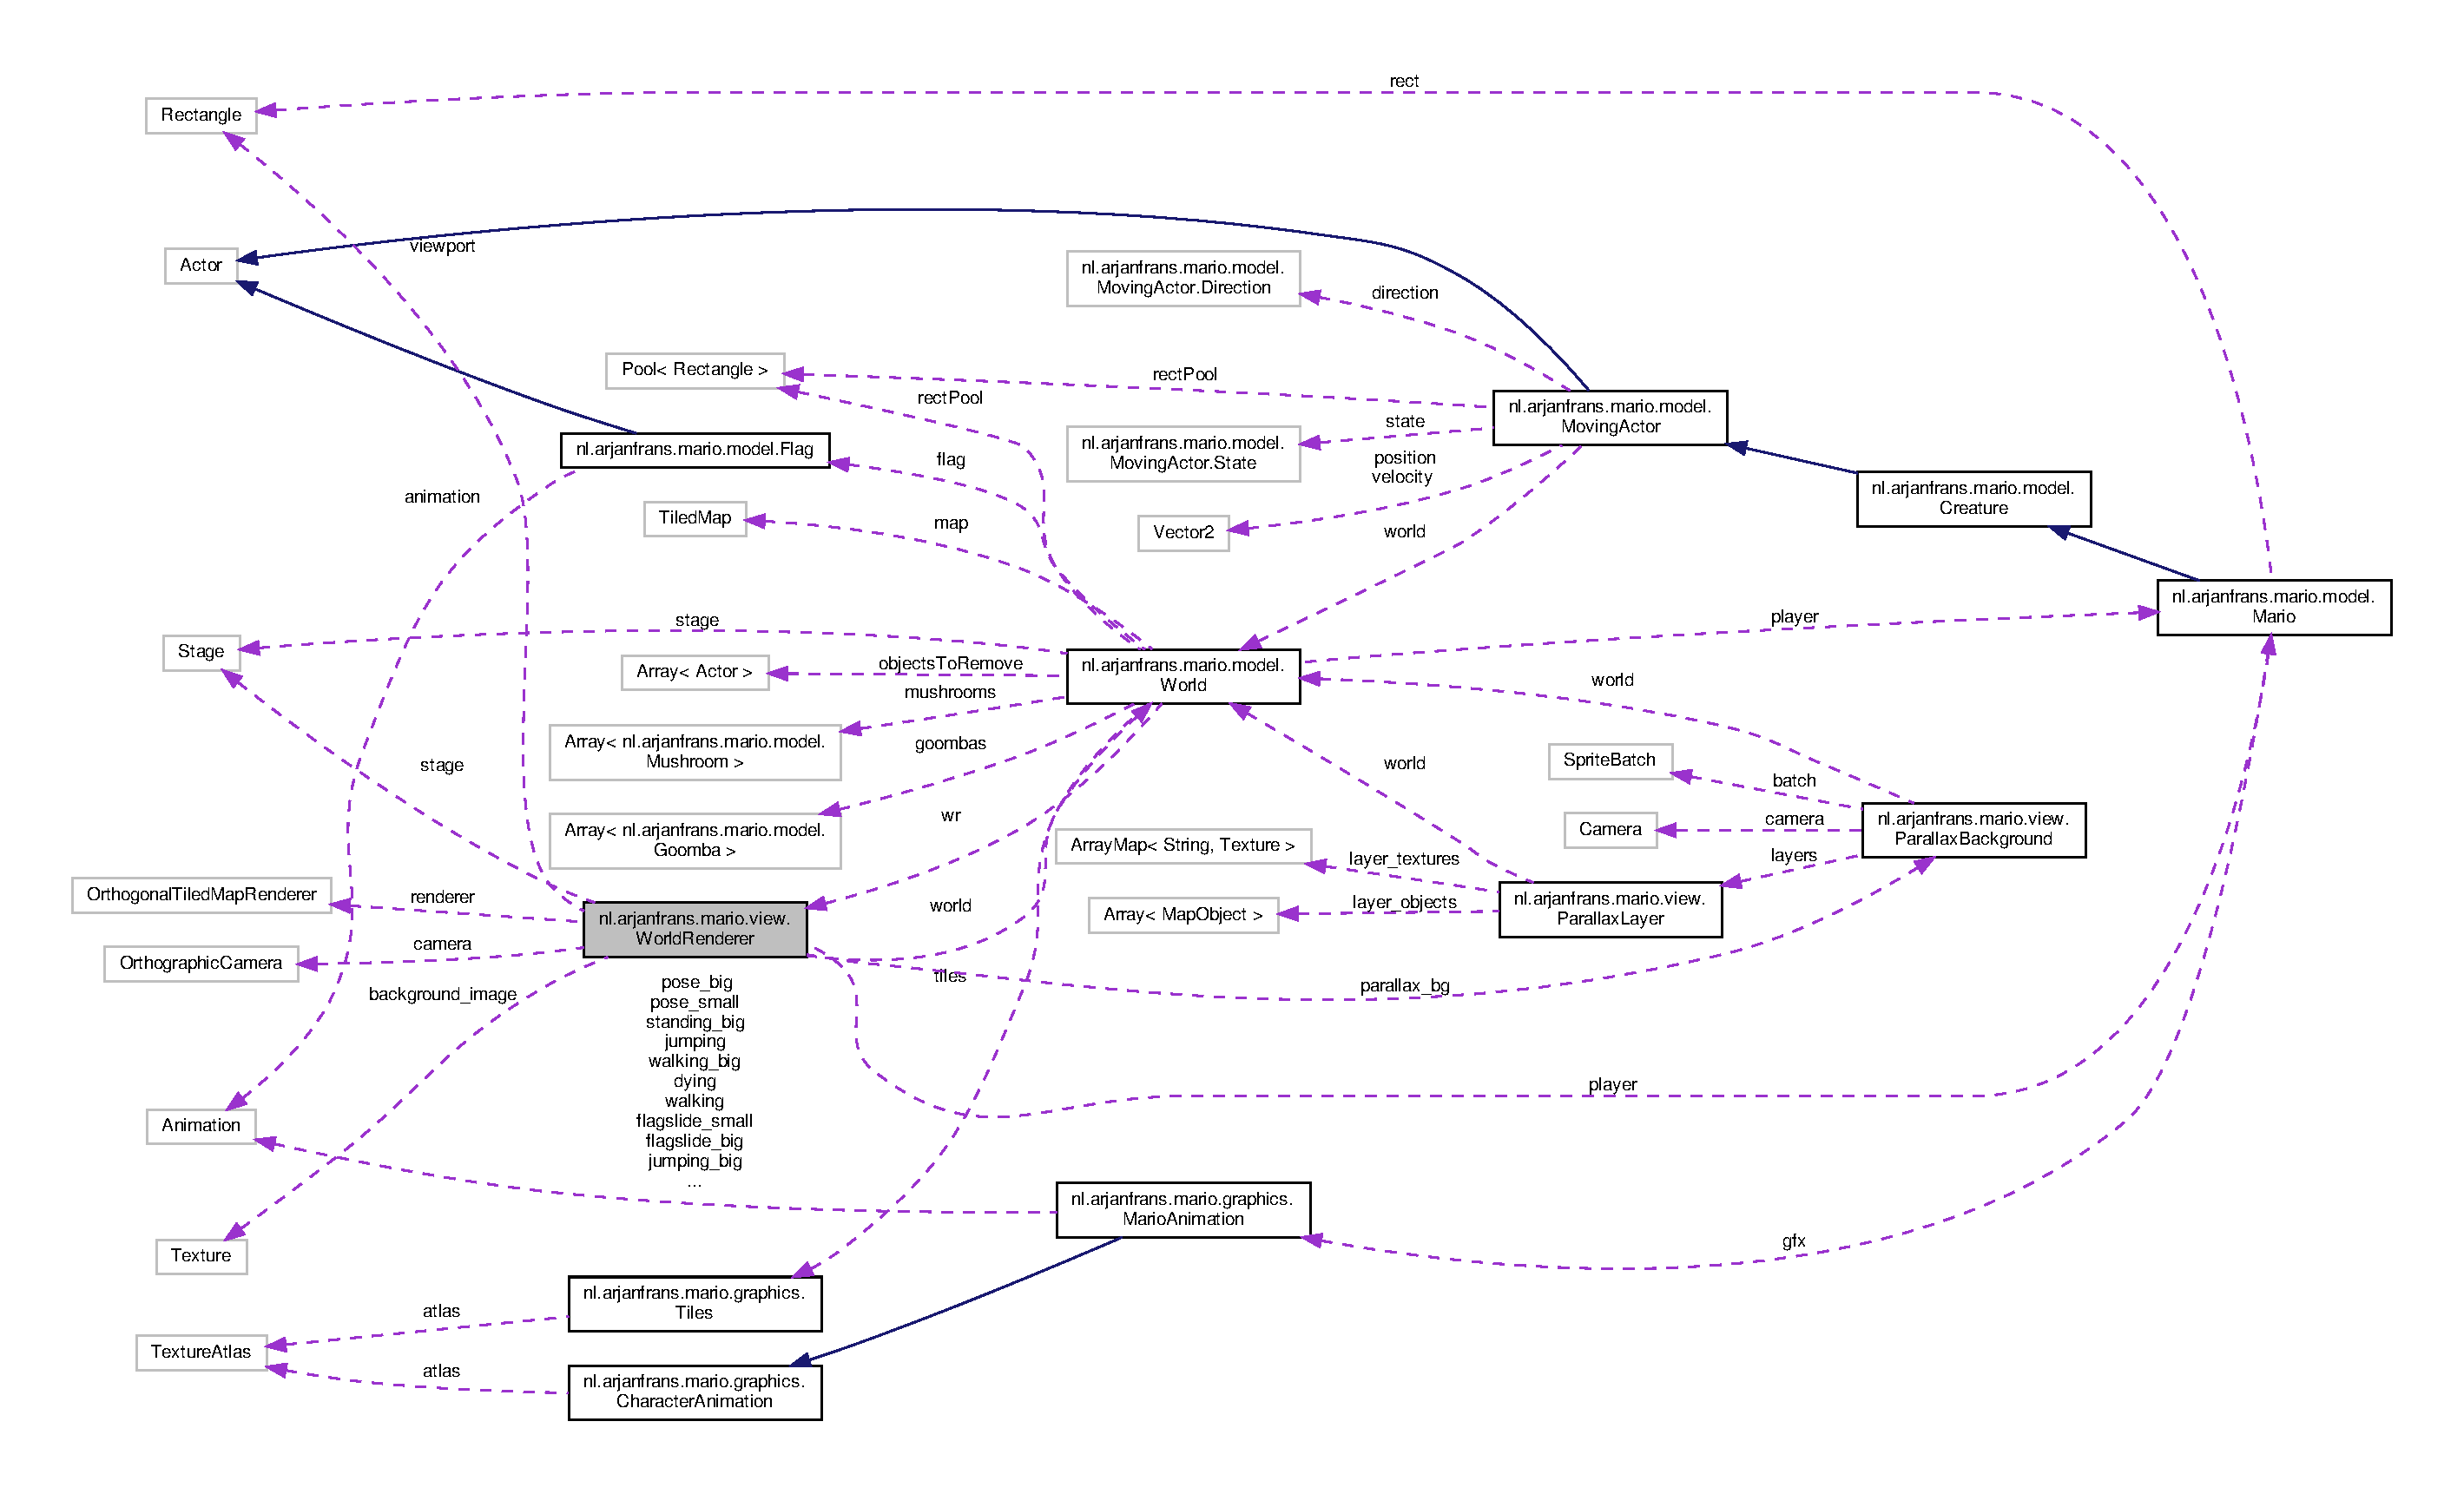
\includegraphics[width=350pt]{classnl_1_1arjanfrans_1_1mario_1_1view_1_1WorldRenderer__coll__graph}
\end{center}
\end{figure}
\subsection*{Public Member Functions}
\begin{DoxyCompactItemize}
\item 
\hyperlink{classnl_1_1arjanfrans_1_1mario_1_1view_1_1WorldRenderer_ae3b0ff5bd619324e74a6656c2a380fc1}{World\+Renderer} (\hyperlink{classnl_1_1arjanfrans_1_1mario_1_1model_1_1World}{World} world)
\begin{DoxyCompactList}\small\item\em Constructor method. \end{DoxyCompactList}\item 
void \hyperlink{classnl_1_1arjanfrans_1_1mario_1_1view_1_1WorldRenderer_a10dcf6ac3ca6c2591648eb560fabb98e}{resize} (int width, int height)
\begin{DoxyCompactList}\small\item\em Set size of viewport. \end{DoxyCompactList}\item 
Orthographic\+Camera \hyperlink{classnl_1_1arjanfrans_1_1mario_1_1view_1_1WorldRenderer_a47406049241a1fef9c68ca9d80db2ee1}{get\+Camera} ()
\begin{DoxyCompactList}\small\item\em Get camera. \end{DoxyCompactList}\item 
\mbox{\Hypertarget{classnl_1_1arjanfrans_1_1mario_1_1view_1_1WorldRenderer_a98341e31f35df9224c43d6a60c4098b4}\label{classnl_1_1arjanfrans_1_1mario_1_1view_1_1WorldRenderer_a98341e31f35df9224c43d6a60c4098b4}} 
void \hyperlink{classnl_1_1arjanfrans_1_1mario_1_1view_1_1WorldRenderer_a98341e31f35df9224c43d6a60c4098b4}{render} ()
\begin{DoxyCompactList}\small\item\em Rendering world. \end{DoxyCompactList}\item 
\mbox{\Hypertarget{classnl_1_1arjanfrans_1_1mario_1_1view_1_1WorldRenderer_a55569f6e8d3f0b9114d7789a6e86fff4}\label{classnl_1_1arjanfrans_1_1mario_1_1view_1_1WorldRenderer_a55569f6e8d3f0b9114d7789a6e86fff4}} 
void \hyperlink{classnl_1_1arjanfrans_1_1mario_1_1view_1_1WorldRenderer_a55569f6e8d3f0b9114d7789a6e86fff4}{dispose} ()
\begin{DoxyCompactList}\small\item\em Disposing render of world. \end{DoxyCompactList}\end{DoxyCompactItemize}
\subsection*{Private Member Functions}
\begin{DoxyCompactItemize}
\item 
Texture \hyperlink{classnl_1_1arjanfrans_1_1mario_1_1view_1_1WorldRenderer_a43f69b3995ab2dc9c82a7c9f78f58821}{load\+Background} ()
\begin{DoxyCompactList}\small\item\em Get texture. \end{DoxyCompactList}\item 
void \hyperlink{classnl_1_1arjanfrans_1_1mario_1_1view_1_1WorldRenderer_a1d8187e70a46eefc5e67a1bec9cfd0cc}{draw\+Background} (Sprite\+Batch batch, float posX, float posY)
\begin{DoxyCompactList}\small\item\em Set background. \end{DoxyCompactList}\end{DoxyCompactItemize}
\subsection*{Private Attributes}
\begin{DoxyCompactItemize}
\item 
\mbox{\Hypertarget{classnl_1_1arjanfrans_1_1mario_1_1view_1_1WorldRenderer_aa2197e07ffe2c9f88fa4083c204598c3}\label{classnl_1_1arjanfrans_1_1mario_1_1view_1_1WorldRenderer_aa2197e07ffe2c9f88fa4083c204598c3}} 
Orthogonal\+Tiled\+Map\+Renderer {\bfseries renderer}
\item 
\mbox{\Hypertarget{classnl_1_1arjanfrans_1_1mario_1_1view_1_1WorldRenderer_a7273f89a16b94bf7aa2cf72c803c3398}\label{classnl_1_1arjanfrans_1_1mario_1_1view_1_1WorldRenderer_a7273f89a16b94bf7aa2cf72c803c3398}} 
Orthographic\+Camera {\bfseries camera}
\item 
\mbox{\Hypertarget{classnl_1_1arjanfrans_1_1mario_1_1view_1_1WorldRenderer_a394a96e12b283c2d9b7e65a8f04d6e18}\label{classnl_1_1arjanfrans_1_1mario_1_1view_1_1WorldRenderer_a394a96e12b283c2d9b7e65a8f04d6e18}} 
\hyperlink{classnl_1_1arjanfrans_1_1mario_1_1model_1_1World}{World} {\bfseries world}
\item 
\mbox{\Hypertarget{classnl_1_1arjanfrans_1_1mario_1_1view_1_1WorldRenderer_aa58f9ae4c8bc74593af23087b8a1b807}\label{classnl_1_1arjanfrans_1_1mario_1_1view_1_1WorldRenderer_aa58f9ae4c8bc74593af23087b8a1b807}} 
\hyperlink{classnl_1_1arjanfrans_1_1mario_1_1model_1_1Mario}{Mario} {\bfseries player}
\item 
\mbox{\Hypertarget{classnl_1_1arjanfrans_1_1mario_1_1view_1_1WorldRenderer_a65bb82b63546ca4248b80fdc96cfa4fb}\label{classnl_1_1arjanfrans_1_1mario_1_1view_1_1WorldRenderer_a65bb82b63546ca4248b80fdc96cfa4fb}} 
Texture {\bfseries background\+\_\+image}
\item 
\mbox{\Hypertarget{classnl_1_1arjanfrans_1_1mario_1_1view_1_1WorldRenderer_ab7def0a19ac69b6ea641506cd26058a6}\label{classnl_1_1arjanfrans_1_1mario_1_1view_1_1WorldRenderer_ab7def0a19ac69b6ea641506cd26058a6}} 
Stage {\bfseries stage}
\item 
\mbox{\Hypertarget{classnl_1_1arjanfrans_1_1mario_1_1view_1_1WorldRenderer_a1ccba4143e804a0c98efaf3f7fafae15}\label{classnl_1_1arjanfrans_1_1mario_1_1view_1_1WorldRenderer_a1ccba4143e804a0c98efaf3f7fafae15}} 
\hyperlink{classnl_1_1arjanfrans_1_1mario_1_1view_1_1ParallaxBackground}{Parallax\+Background} {\bfseries parallax\+\_\+bg}
\item 
\mbox{\Hypertarget{classnl_1_1arjanfrans_1_1mario_1_1view_1_1WorldRenderer_a66cdb6ceed6dc725b346ba0a07ad3bdf}\label{classnl_1_1arjanfrans_1_1mario_1_1view_1_1WorldRenderer_a66cdb6ceed6dc725b346ba0a07ad3bdf}} 
Rectangle {\bfseries viewport}
\end{DoxyCompactItemize}
\subsection*{Static Private Attributes}
\begin{DoxyCompactItemize}
\item 
\mbox{\Hypertarget{classnl_1_1arjanfrans_1_1mario_1_1view_1_1WorldRenderer_abcb78ea8c0477db3aa4fd48b651d6bd5}\label{classnl_1_1arjanfrans_1_1mario_1_1view_1_1WorldRenderer_abcb78ea8c0477db3aa4fd48b651d6bd5}} 
static final int {\bfseries V\+I\+R\+T\+U\+A\+L\+\_\+\+W\+I\+D\+TH} = 512
\item 
\mbox{\Hypertarget{classnl_1_1arjanfrans_1_1mario_1_1view_1_1WorldRenderer_a9823fdab35ee11e7fce194a0947e4833}\label{classnl_1_1arjanfrans_1_1mario_1_1view_1_1WorldRenderer_a9823fdab35ee11e7fce194a0947e4833}} 
static final int {\bfseries V\+I\+R\+T\+U\+A\+L\+\_\+\+H\+E\+I\+G\+HT} = 448
\item 
\mbox{\Hypertarget{classnl_1_1arjanfrans_1_1mario_1_1view_1_1WorldRenderer_afa106e71dbcc30e726ae1d3a211a0397}\label{classnl_1_1arjanfrans_1_1mario_1_1view_1_1WorldRenderer_afa106e71dbcc30e726ae1d3a211a0397}} 
static final float {\bfseries A\+S\+P\+E\+C\+T\+\_\+\+R\+A\+T\+IO} = (float)V\+I\+R\+T\+U\+A\+L\+\_\+\+W\+I\+D\+TH/(float)V\+I\+R\+T\+U\+A\+L\+\_\+\+H\+E\+I\+G\+HT
\end{DoxyCompactItemize}


\subsection{Detailed Description}
Render of world. 

\subsection{Constructor \& Destructor Documentation}
\mbox{\Hypertarget{classnl_1_1arjanfrans_1_1mario_1_1view_1_1WorldRenderer_ae3b0ff5bd619324e74a6656c2a380fc1}\label{classnl_1_1arjanfrans_1_1mario_1_1view_1_1WorldRenderer_ae3b0ff5bd619324e74a6656c2a380fc1}} 
\index{nl\+::arjanfrans\+::mario\+::view\+::\+World\+Renderer@{nl\+::arjanfrans\+::mario\+::view\+::\+World\+Renderer}!World\+Renderer@{World\+Renderer}}
\index{World\+Renderer@{World\+Renderer}!nl\+::arjanfrans\+::mario\+::view\+::\+World\+Renderer@{nl\+::arjanfrans\+::mario\+::view\+::\+World\+Renderer}}
\subsubsection{\texorpdfstring{World\+Renderer()}{WorldRenderer()}}
{\footnotesize\ttfamily nl.\+arjanfrans.\+mario.\+view.\+World\+Renderer.\+World\+Renderer (\begin{DoxyParamCaption}\item[{\hyperlink{classnl_1_1arjanfrans_1_1mario_1_1model_1_1World}{World}}]{world }\end{DoxyParamCaption})}



Constructor method. 

Method which initializes an instance of \hyperlink{classnl_1_1arjanfrans_1_1mario_1_1view_1_1WorldRenderer}{World\+Renderer} 
\begin{DoxyParams}{Parameters}
{\em world} & The world object in which Mario will exist in \\
\hline
\end{DoxyParams}


\subsection{Member Function Documentation}
\mbox{\Hypertarget{classnl_1_1arjanfrans_1_1mario_1_1view_1_1WorldRenderer_a1d8187e70a46eefc5e67a1bec9cfd0cc}\label{classnl_1_1arjanfrans_1_1mario_1_1view_1_1WorldRenderer_a1d8187e70a46eefc5e67a1bec9cfd0cc}} 
\index{nl\+::arjanfrans\+::mario\+::view\+::\+World\+Renderer@{nl\+::arjanfrans\+::mario\+::view\+::\+World\+Renderer}!draw\+Background@{draw\+Background}}
\index{draw\+Background@{draw\+Background}!nl\+::arjanfrans\+::mario\+::view\+::\+World\+Renderer@{nl\+::arjanfrans\+::mario\+::view\+::\+World\+Renderer}}
\subsubsection{\texorpdfstring{draw\+Background()}{drawBackground()}}
{\footnotesize\ttfamily void nl.\+arjanfrans.\+mario.\+view.\+World\+Renderer.\+draw\+Background (\begin{DoxyParamCaption}\item[{Sprite\+Batch}]{batch,  }\item[{float}]{posX,  }\item[{float}]{posY }\end{DoxyParamCaption})\hspace{0.3cm}{\ttfamily [private]}}



Set background. 


\begin{DoxyParams}{Parameters}
{\em batch} & Sprite\+Batch object \\
\hline
{\em posX} & coordinate \\
\hline
{\em posY} & coordinate \\
\hline
\end{DoxyParams}
\mbox{\Hypertarget{classnl_1_1arjanfrans_1_1mario_1_1view_1_1WorldRenderer_a47406049241a1fef9c68ca9d80db2ee1}\label{classnl_1_1arjanfrans_1_1mario_1_1view_1_1WorldRenderer_a47406049241a1fef9c68ca9d80db2ee1}} 
\index{nl\+::arjanfrans\+::mario\+::view\+::\+World\+Renderer@{nl\+::arjanfrans\+::mario\+::view\+::\+World\+Renderer}!get\+Camera@{get\+Camera}}
\index{get\+Camera@{get\+Camera}!nl\+::arjanfrans\+::mario\+::view\+::\+World\+Renderer@{nl\+::arjanfrans\+::mario\+::view\+::\+World\+Renderer}}
\subsubsection{\texorpdfstring{get\+Camera()}{getCamera()}}
{\footnotesize\ttfamily Orthographic\+Camera nl.\+arjanfrans.\+mario.\+view.\+World\+Renderer.\+get\+Camera (\begin{DoxyParamCaption}{ }\end{DoxyParamCaption})}



Get camera. 

\begin{DoxyReturn}{Returns}
camera Orthographic\+Camera object 
\end{DoxyReturn}
\mbox{\Hypertarget{classnl_1_1arjanfrans_1_1mario_1_1view_1_1WorldRenderer_a43f69b3995ab2dc9c82a7c9f78f58821}\label{classnl_1_1arjanfrans_1_1mario_1_1view_1_1WorldRenderer_a43f69b3995ab2dc9c82a7c9f78f58821}} 
\index{nl\+::arjanfrans\+::mario\+::view\+::\+World\+Renderer@{nl\+::arjanfrans\+::mario\+::view\+::\+World\+Renderer}!load\+Background@{load\+Background}}
\index{load\+Background@{load\+Background}!nl\+::arjanfrans\+::mario\+::view\+::\+World\+Renderer@{nl\+::arjanfrans\+::mario\+::view\+::\+World\+Renderer}}
\subsubsection{\texorpdfstring{load\+Background()}{loadBackground()}}
{\footnotesize\ttfamily Texture nl.\+arjanfrans.\+mario.\+view.\+World\+Renderer.\+load\+Background (\begin{DoxyParamCaption}{ }\end{DoxyParamCaption})\hspace{0.3cm}{\ttfamily [private]}}



Get texture. 

\begin{DoxyReturn}{Returns}
texture of world 
\end{DoxyReturn}
\mbox{\Hypertarget{classnl_1_1arjanfrans_1_1mario_1_1view_1_1WorldRenderer_a10dcf6ac3ca6c2591648eb560fabb98e}\label{classnl_1_1arjanfrans_1_1mario_1_1view_1_1WorldRenderer_a10dcf6ac3ca6c2591648eb560fabb98e}} 
\index{nl\+::arjanfrans\+::mario\+::view\+::\+World\+Renderer@{nl\+::arjanfrans\+::mario\+::view\+::\+World\+Renderer}!resize@{resize}}
\index{resize@{resize}!nl\+::arjanfrans\+::mario\+::view\+::\+World\+Renderer@{nl\+::arjanfrans\+::mario\+::view\+::\+World\+Renderer}}
\subsubsection{\texorpdfstring{resize()}{resize()}}
{\footnotesize\ttfamily void nl.\+arjanfrans.\+mario.\+view.\+World\+Renderer.\+resize (\begin{DoxyParamCaption}\item[{int}]{width,  }\item[{int}]{height }\end{DoxyParamCaption})}



Set size of viewport. 

Adjust size of world 
\begin{DoxyParams}{Parameters}
{\em width} & of window \\
\hline
{\em height} & of window \\
\hline
\end{DoxyParams}


The documentation for this class was generated from the following file\+:\begin{DoxyCompactItemize}
\item 
core/src/nl/arjanfrans/mario/view/\hyperlink{WorldRenderer_8java}{World\+Renderer.\+java}\end{DoxyCompactItemize}

\chapter{File Documentation}
\hypertarget{ActorActions_8java}{}\section{core/src/nl/arjanfrans/mario/actions/\+Actor\+Actions.java File Reference}
\label{ActorActions_8java}\index{core/src/nl/arjanfrans/mario/actions/\+Actor\+Actions.\+java@{core/src/nl/arjanfrans/mario/actions/\+Actor\+Actions.\+java}}
\subsection*{Classes}
\begin{DoxyCompactItemize}
\item 
class \hyperlink{classnl_1_1arjanfrans_1_1mario_1_1actions_1_1ActorActions}{nl.\+arjanfrans.\+mario.\+actions.\+Actor\+Actions}
\begin{DoxyCompactList}\small\item\em Inherited class Actions. \end{DoxyCompactList}\item 
class {\bfseries nl.\+arjanfrans.\+mario.\+actions.\+Actor\+Actions.\+remove\+Actor}
\begin{DoxyCompactList}\small\item\em Inherited class Action. \end{DoxyCompactList}\end{DoxyCompactItemize}

\hypertarget{MarioActions_8java}{}\section{core/src/nl/arjanfrans/mario/actions/\+Mario\+Actions.java File Reference}
\label{MarioActions_8java}\index{core/src/nl/arjanfrans/mario/actions/\+Mario\+Actions.\+java@{core/src/nl/arjanfrans/mario/actions/\+Mario\+Actions.\+java}}
\subsection*{Classes}
\begin{DoxyCompactItemize}
\item 
class \hyperlink{classnl_1_1arjanfrans_1_1mario_1_1actions_1_1MarioActions}{nl.\+arjanfrans.\+mario.\+actions.\+Mario\+Actions}
\begin{DoxyCompactList}\small\item\em Inherited class Actions. \end{DoxyCompactList}\item 
class {\bfseries nl.\+arjanfrans.\+mario.\+actions.\+Mario\+Actions.\+stop\+Immume}
\begin{DoxyCompactList}\small\item\em Inherited class Action. \end{DoxyCompactList}\item 
class {\bfseries nl.\+arjanfrans.\+mario.\+actions.\+Mario\+Actions.\+big\+Mario}
\begin{DoxyCompactList}\small\item\em Inherited class Action. \end{DoxyCompactList}\item 
class {\bfseries nl.\+arjanfrans.\+mario.\+actions.\+Mario\+Actions.\+flag\+Take\+Down}
\begin{DoxyCompactList}\small\item\em Inherited class Action. \end{DoxyCompactList}\item 
class {\bfseries nl.\+arjanfrans.\+mario.\+actions.\+Mario\+Actions.\+finish\+Level}
\begin{DoxyCompactList}\small\item\em Inherited class Action. \end{DoxyCompactList}\item 
class {\bfseries nl.\+arjanfrans.\+mario.\+actions.\+Mario\+Actions.\+set\+State}
\begin{DoxyCompactList}\small\item\em Inherited class Action. \end{DoxyCompactList}\item 
class {\bfseries nl.\+arjanfrans.\+mario.\+actions.\+Mario\+Actions.\+walk\+To}
\begin{DoxyCompactList}\small\item\em Inherited class Action. \end{DoxyCompactList}\end{DoxyCompactItemize}

\hypertarget{MoveableActions_8java}{}\section{core/src/nl/arjanfrans/mario/actions/\+Moveable\+Actions.java File Reference}
\label{MoveableActions_8java}\index{core/src/nl/arjanfrans/mario/actions/\+Moveable\+Actions.\+java@{core/src/nl/arjanfrans/mario/actions/\+Moveable\+Actions.\+java}}
\subsection*{Classes}
\begin{DoxyCompactItemize}
\item 
class \hyperlink{classnl_1_1arjanfrans_1_1mario_1_1actions_1_1MoveableActions}{nl.\+arjanfrans.\+mario.\+actions.\+Moveable\+Actions}
\begin{DoxyCompactList}\small\item\em Inherited class Actions. \end{DoxyCompactList}\item 
class {\bfseries nl.\+arjanfrans.\+mario.\+actions.\+Moveable\+Actions.\+Die}
\begin{DoxyCompactList}\small\item\em Inherited class Action. \end{DoxyCompactList}\item 
class {\bfseries nl.\+arjanfrans.\+mario.\+actions.\+Moveable\+Actions.\+start\+Moving}
\begin{DoxyCompactList}\small\item\em Inherited class Action. \end{DoxyCompactList}\end{DoxyCompactItemize}

\hypertarget{D_8java}{}\section{core/src/nl/arjanfrans/mario/debug/D.java File Reference}
\label{D_8java}\index{core/src/nl/arjanfrans/mario/debug/\+D.\+java@{core/src/nl/arjanfrans/mario/debug/\+D.\+java}}
\subsection*{Classes}
\begin{DoxyCompactItemize}
\item 
class \hyperlink{classnl_1_1arjanfrans_1_1mario_1_1debug_1_1D}{nl.\+arjanfrans.\+mario.\+debug.\+D}
\begin{DoxyCompactList}\small\item\em Debug class. \end{DoxyCompactList}\end{DoxyCompactItemize}

\hypertarget{MarioInput_8java}{}\section{core/src/nl/arjanfrans/mario/input/\+Mario\+Input.java File Reference}
\label{MarioInput_8java}\index{core/src/nl/arjanfrans/mario/input/\+Mario\+Input.\+java@{core/src/nl/arjanfrans/mario/input/\+Mario\+Input.\+java}}
\subsection*{Classes}
\begin{DoxyCompactItemize}
\item 
class \hyperlink{classnl_1_1arjanfrans_1_1mario_1_1input_1_1MarioInput}{nl.\+arjanfrans.\+mario.\+input.\+Mario\+Input}
\begin{DoxyCompactList}\small\item\em Inherited class that overrides mario input methods. \end{DoxyCompactList}\end{DoxyCompactItemize}

\hypertarget{Creature_8java}{}\section{core/src/nl/arjanfrans/mario/model/\+Creature.java File Reference}
\label{Creature_8java}\index{core/src/nl/arjanfrans/mario/model/\+Creature.\+java@{core/src/nl/arjanfrans/mario/model/\+Creature.\+java}}
\subsection*{Classes}
\begin{DoxyCompactItemize}
\item 
class \hyperlink{classnl_1_1arjanfrans_1_1mario_1_1model_1_1Creature}{nl.\+arjanfrans.\+mario.\+model.\+Creature}
\begin{DoxyCompactList}\small\item\em This class is the class model to represent any moving actor that is interactive, and not \hyperlink{classnl_1_1arjanfrans_1_1mario_1_1model_1_1Mario}{Mario}. \end{DoxyCompactList}\end{DoxyCompactItemize}

\hypertarget{Flag_8java}{}\section{core/src/nl/arjanfrans/mario/model/\+Flag.java File Reference}
\label{Flag_8java}\index{core/src/nl/arjanfrans/mario/model/\+Flag.\+java@{core/src/nl/arjanfrans/mario/model/\+Flag.\+java}}
\subsection*{Classes}
\begin{DoxyCompactItemize}
\item 
class \hyperlink{classnl_1_1arjanfrans_1_1mario_1_1model_1_1Flag}{nl.\+arjanfrans.\+mario.\+model.\+Flag}
\begin{DoxyCompactList}\small\item\em This flag represents the flag pole at the end of the stage that completes if \hyperlink{classnl_1_1arjanfrans_1_1mario_1_1model_1_1Mario}{Mario} interacts with it. \end{DoxyCompactList}\end{DoxyCompactItemize}

\hypertarget{Goomba_8java}{}\section{core/src/nl/arjanfrans/mario/model/\+Goomba.java File Reference}
\label{Goomba_8java}\index{core/src/nl/arjanfrans/mario/model/\+Goomba.\+java@{core/src/nl/arjanfrans/mario/model/\+Goomba.\+java}}
\subsection*{Classes}
\begin{DoxyCompactItemize}
\item 
class \hyperlink{classnl_1_1arjanfrans_1_1mario_1_1model_1_1Goomba}{nl.\+arjanfrans.\+mario.\+model.\+Goomba}
\begin{DoxyCompactList}\small\item\em \hyperlink{classnl_1_1arjanfrans_1_1mario_1_1model_1_1Goomba}{Goomba} represents the \hyperlink{classnl_1_1arjanfrans_1_1mario_1_1model_1_1Goomba}{Goomba} enemies from the original \hyperlink{classnl_1_1arjanfrans_1_1mario_1_1model_1_1Mario}{Mario} game. \end{DoxyCompactList}\end{DoxyCompactItemize}

\hypertarget{Item_8java}{}\section{core/src/nl/arjanfrans/mario/model/\+Item.java File Reference}
\label{Item_8java}\index{core/src/nl/arjanfrans/mario/model/\+Item.\+java@{core/src/nl/arjanfrans/mario/model/\+Item.\+java}}
\subsection*{Classes}
\begin{DoxyCompactItemize}
\item 
class \hyperlink{classnl_1_1arjanfrans_1_1mario_1_1model_1_1Item}{nl.\+arjanfrans.\+mario.\+model.\+Item}
\begin{DoxyCompactList}\small\item\em Represents any item in game. \end{DoxyCompactList}\end{DoxyCompactItemize}

\hypertarget{Mario_8java}{}\section{core/src/nl/arjanfrans/mario/model/\+Mario.java File Reference}
\label{Mario_8java}\index{core/src/nl/arjanfrans/mario/model/\+Mario.\+java@{core/src/nl/arjanfrans/mario/model/\+Mario.\+java}}
\subsection*{Classes}
\begin{DoxyCompactItemize}
\item 
class \hyperlink{classnl_1_1arjanfrans_1_1mario_1_1model_1_1Mario}{nl.\+arjanfrans.\+mario.\+model.\+Mario}
\begin{DoxyCompactList}\small\item\em Represents the playable character in the game. \end{DoxyCompactList}\end{DoxyCompactItemize}

\hypertarget{Mushroom_8java}{}\section{core/src/nl/arjanfrans/mario/model/\+Mushroom.java File Reference}
\label{Mushroom_8java}\index{core/src/nl/arjanfrans/mario/model/\+Mushroom.\+java@{core/src/nl/arjanfrans/mario/model/\+Mushroom.\+java}}
\subsection*{Classes}
\begin{DoxyCompactItemize}
\item 
class \hyperlink{classnl_1_1arjanfrans_1_1mario_1_1model_1_1Mushroom}{nl.\+arjanfrans.\+mario.\+model.\+Mushroom}
\begin{DoxyCompactList}\small\item\em Inherited class \hyperlink{classnl_1_1arjanfrans_1_1mario_1_1model_1_1MovingActor}{Moving\+Actor}. \end{DoxyCompactList}\end{DoxyCompactItemize}

\hypertarget{StaticActor_8java}{}\section{core/src/nl/arjanfrans/mario/model/\+Static\+Actor.java File Reference}
\label{StaticActor_8java}\index{core/src/nl/arjanfrans/mario/model/\+Static\+Actor.\+java@{core/src/nl/arjanfrans/mario/model/\+Static\+Actor.\+java}}
\subsection*{Classes}
\begin{DoxyCompactItemize}
\item 
class \hyperlink{classnl_1_1arjanfrans_1_1mario_1_1model_1_1StaticActor}{nl.\+arjanfrans.\+mario.\+model.\+Static\+Actor}
\begin{DoxyCompactList}\small\item\em Inherited class that represents static actor. \end{DoxyCompactList}\end{DoxyCompactItemize}

\hypertarget{Super_8java}{}\section{core/src/nl/arjanfrans/mario/model/\+Super.java File Reference}
\label{Super_8java}\index{core/src/nl/arjanfrans/mario/model/\+Super.\+java@{core/src/nl/arjanfrans/mario/model/\+Super.\+java}}
\subsection*{Classes}
\begin{DoxyCompactItemize}
\item 
class \hyperlink{classnl_1_1arjanfrans_1_1mario_1_1model_1_1Super}{nl.\+arjanfrans.\+mario.\+model.\+Super}
\begin{DoxyCompactList}\small\item\em Inherited class that overrides \hyperlink{classnl_1_1arjanfrans_1_1mario_1_1model_1_1Mushroom}{Mushroom} methods that represents mario in super state. \end{DoxyCompactList}\end{DoxyCompactItemize}

\hypertarget{World_8java}{}\section{core/src/nl/arjanfrans/mario/model/\+World.java File Reference}
\label{World_8java}\index{core/src/nl/arjanfrans/mario/model/\+World.\+java@{core/src/nl/arjanfrans/mario/model/\+World.\+java}}
\subsection*{Classes}
\begin{DoxyCompactItemize}
\item 
class \hyperlink{classnl_1_1arjanfrans_1_1mario_1_1model_1_1World}{nl.\+arjanfrans.\+mario.\+model.\+World}
\begin{DoxyCompactList}\small\item\em Represents world. \end{DoxyCompactList}\end{DoxyCompactItemize}

\hypertarget{WorldRenderer_8java}{}\section{core/src/nl/arjanfrans/mario/view/\+World\+Renderer.java File Reference}
\label{WorldRenderer_8java}\index{core/src/nl/arjanfrans/mario/view/\+World\+Renderer.\+java@{core/src/nl/arjanfrans/mario/view/\+World\+Renderer.\+java}}
\subsection*{Classes}
\begin{DoxyCompactItemize}
\item 
class \hyperlink{classnl_1_1arjanfrans_1_1mario_1_1view_1_1WorldRenderer}{nl.\+arjanfrans.\+mario.\+view.\+World\+Renderer}
\begin{DoxyCompactList}\small\item\em Render of world. \end{DoxyCompactList}\end{DoxyCompactItemize}

\hypertarget{DesktopLauncher_8java}{}\section{desktop/src/nl/arjanfrans/mario/desktop/\+Desktop\+Launcher.java File Reference}
\label{DesktopLauncher_8java}\index{desktop/src/nl/arjanfrans/mario/desktop/\+Desktop\+Launcher.\+java@{desktop/src/nl/arjanfrans/mario/desktop/\+Desktop\+Launcher.\+java}}
\subsection*{Classes}
\begin{DoxyCompactItemize}
\item 
class \hyperlink{classnl_1_1arjanfrans_1_1mario_1_1desktop_1_1DesktopLauncher}{nl.\+arjanfrans.\+mario.\+desktop.\+Desktop\+Launcher}
\begin{DoxyCompactList}\small\item\em This class is the main method allowing the game to initialize and launch. \end{DoxyCompactList}\end{DoxyCompactItemize}

%--- End generated contents ---

% Index
\backmatter
\newpage
\phantomsection
\clearemptydoublepage
\addcontentsline{toc}{chapter}{Index}
\printindex

\end{document}
